\documentclass[12pt]{amsart}
\usepackage[margin=1in]{geometry}
\usepackage{amsmath,amssymb,multicol,graphicx,framed,ifthen,stmaryrd,enumitem,colonequals,lettrine,comment}
\usepackage{kpfonts,baskervald}
\usepackage{color}
\definecolor{chianti}{rgb}{0.6,0,0}
\definecolor{meretale}{rgb}{0,0,.6}
\definecolor{leaf}{rgb}{0,.35,0}
\usepackage[colorlinks=true, pagebackref, hyperindex, citecolor=meretale, urlcolor=leaf,linkcolor=chianti,hyperfootnotes=false]{hyperref}

\usepackage{enumitem}
\setlist[enumerate,1]{label={(\arabic*)}}
%\usepackage{stmaryrd}
%\usepackage{color}


\usepackage{mathtools}
\usepackage{tikz}
\usetikzlibrary{shapes.geometric}
\newcommand{\Ngon}[2][]{\vcenter{\hbox{\begin{tikzpicture}
\node[regular polygon, regular polygon sides=#2, draw,minimum size=2cm,#1](#2-gon){};
\foreach \X in {1,...,#2}{\fill (#2-gon.corner \X) circle[radius=2pt];}
\end{tikzpicture}}}}

\definecolor{mycolor}{rgb}{0, 0.5, 0.74}

\usepackage{extarrows}
\usepackage{imakeidx}
\usepackage{tikz}
\usepackage{pdflscape}
\usepackage{centernot,colonequals,cleveref}
\usepackage[bottom]{footmisc}
\usepackage[color,matrix,arrow]{xy}
%\UseTwocells  
\xyoption{rotate}
\xyoption{pdf}



\newtheorem{theorem}{Theorem}[chapter]
\newtheorem*{theorem*}{Theorem}
\newtheorem{lemma}[theorem]{Lemma}
\newtheorem{proposition}[theorem]{Proposition}
\newtheorem{corollary}[theorem]{Corollary}
\newtheorem{conjecture}[theorem]{Conjecture}
\newtheorem{Example}[theorem]{Example}
\newtheorem{metatheorem}[theorem]{Metatheorem}
\numberwithin{equation}{section}
\numberwithin{theorem}{chapter}
\newtheorem{problem}[theorem]{Problem}


\newtheorem*{thmnonumber}{Theorem}

\theoremstyle{definition}
\newtheorem{definition}[theorem]{Definition}
\newtheorem{fuzzydefn}[theorem]{Informal definition}
\newtheorem{propdef}[theorem]{Proposition--Definition}
\newtheorem{discussion}[theorem]{Discussion}
\newtheorem{question}[theorem]{Question}
\newtheorem{example}[theorem]{Example}
\newtheorem{exercise}{Exercise}
\newtheorem*{basic properties}{Basic Properties}
\newtheorem*{properties}{Properties}
\newtheorem*{eremarks}{Ending Remarks}
\newtheorem*{Important Remark}{Important Remark}
\newtheorem{remark}[theorem]{Remark}
\newtheorem{construction}[theorem]{Construction}
\newtheorem{axiom}[theorem]{Axiom}

%\theoremstyle{remark}
\newtheorem*{claim*}{Claim}
\newtheorem{setup}[theorem]{Set up}
\newtheorem{algorithm}[theorem]{Algorithm}
\newtheorem{notation}[theorem]{Notation}
\newtheorem*{m2}{Macaulay2}
\newtheorem{observation}[theorem]{Observation}


%important: definitions for the index
\newcommand{\df}[1]{{\bf #1}\index{#1}}


\DeclareMathOperator{\rank}{rank}
\DeclareMathOperator{\Gal}{Gal}
\DeclareMathOperator{\Fun}{Fun}
\DeclareMathOperator{\GL}{GL}
\DeclareMathOperator{\SL}{SL}
\DeclareMathOperator{\Perm}{Perm}
\DeclareMathOperator{\sign}{sign}


%For sets
\newcommand{\set}[1]{\left\{ #1 \right\}}
\newcommand{\R}{\mathbb{R}}
\newcommand{\N}{\mathbb{N}}
\newcommand{\Z}{\mathbb{Z}}
\newcommand{\Q}{\mathbb{Q}}
\newcommand{\F}{\mathbb{F}}
\newcommand{\C}{\mathbb{C}}
\newcommand{\cS}{\mathcal{S}}
\def\sdp{\rtimes}

\renewcommand{\ker}{\operatorname{ker}}
\newcommand{\coker}{\operatorname{coker}}
\DeclareMathOperator{\im}{im}
\DeclareMathOperator{\id}{id}
\DeclareMathOperator{\Aut}{Aut}
\DeclareMathOperator{\Orb}{Orb}
\DeclareMathOperator{\lcm}{lcm}
\def\norm{\mathrel{\unlhd}}
\DeclareMathOperator{\Zc}{Z}
\DeclareMathOperator{\Stab}{Stab}
\DeclareMathOperator{\Syl}{Syl}

\DeclareMathOperator{\Mat}{Mat}
\DeclareMathOperator{\End}{End}
\DeclareMathOperator{\lc}{lc}
\DeclareMathOperator{\Frac}{Frac}
\DeclareMathOperator{\Hom}{Hom}

\newcommand{\Tr}{\operatorname{Tr}}
\DeclareMathOperator{\Span}{span}
\DeclareMathOperator{\M}{Mat}
\DeclareMathOperator{\ann}{ann}
\DeclareMathOperator{\Tor}{Tor}
\DeclareMathOperator{\ch}{char}


\def\nsg{\unlhd}

\newcommand{\cZ}{\mathcal{Z}}
\newcommand{\cI}{\mathcal{I}}
\newcommand{\cP}{\mathcal{P}}
\newcommand{\cT}{\mathcal{T}}
\newcommand{\m}{\mathfrak{m}}

\newcommand{\s}{\sigma}




\begin{document}



hi




\newpage


\pagenumbering{arabic}



\part{Groups}



\begin{comment}

{Groups: an introduction}

Many mathematical structures consist of a set with special properties. Groups are elementary algebraic structures that allow us to deal with many objects of interest, such as geometric shapes and polynomials.

\section{Definitions and first examples}

\begin{definition}
A \df{binary operation} on a set $S$ is a function $S \times S \to S$. If the binary operation is denoted by $\cdot$, we write $x \cdot y$ for the image of $(x,y)$ under the binary operation $\cdot$.
%$$
%- \cdot -: S \times S \to S, \, \text{ given by $(x,y) \mapsto x \cdot y$}.
%$$
	
\end{definition}
 
\begin{remark}
We often write $xy$ instead of $x \cdot y$ if the operation is clear from context.
\end{remark}

\begin{remark} 
We say that that a set $S$ is closed under the operation $\cdot$ when we want to emphasize that for any $x,y\in S$ the result $xy$ of the operation is an element of $S$.  But note that closure is really part of the definition of a binary operation on a set, and it is implicitly assumed whenever we consider such an operation.
\end{remark}


\begin{definition}\label{def:group} 
A \df{group} is a set $G$ equipped with a binary operation $\cdot$ on $G$ called the {\bf group multiplication}, satisfying the following properties:
\begin{itemize}
\item Associativity: For every $x,y,z \in G$, we have $(x \cdot y) \cdot z = x \cdot (y \cdot z)$.
\item Identity element: There exists $e \in G$ such that $e \cdot x = x \cdot e = x$ for all $x \in G$.
 \item Inverses: For each $x \in G$, there is an element $y \in G$ such that $xy = e = yx$ .
\end{itemize}
The element $e$ is called the \df{identity element} or simply \df{identity} of the group. For each element $x \in G$, an element $y \in G$ such that $xy = e = yx$ is called an \df{inverse} of $x$. We may write that $(G, \cdot)$ is a group to mean that $G$ is a group with the operation $\cdot$.

The {\bf order} of the group $G$ is the number of elements in the underlying set.\index{order of a group}
\end{definition}

\begin{remark}
Although a group is the set \emph{and} the operation, we will usually refer to the group by only naming the underlying set, $G$.
\end{remark}

\begin{remark} 
A set $G$ equipped with an associative binary operation is a \df{semigroup}; if a semigroup also has an identity element, it is a \df{monoid}. 

While \emph{we will not be discussing semigroups nor monoids that are not groups in this class}, they can be useful and interesting objects. We will however include some fun facts about monoids in the remarks. In particular, there will be no monoids whatsoever in the qualifying exam.
\end{remark}


\begin{lemma}\label{identity and inverses unique}
For any group $G$, we have the following properties:
  \begin{enumerate}
  \item The identity is unique: there exists a unique $e \in G$ with $ex = x = xe$ for all $x \in G$.
  \item Inverses are unique: for each $x \in G$, there exists a unique $y \in G$ such that $xy=e=yx$.
    \end{enumerate}
\end{lemma}

\begin{proof}
Suppose $e$ and $e'$ are two identity elements; that is, assume $e$ and $e'$ satisfy $ex = x = xe$ and $e'x = x = xe'$ for all $x \in G$. Then 
$$e = ee' = e'.$$ 

Now given $x \in G$, suppose $y$ and $z$ are two inverses for $x$, meaning that $yx = xy = e$ and $zx = xz = e$. Then 
$$\begin{aligned}
z & = ez &&& \textrm{since $e$ is the identity}\\
& = (yx)z &&& \textrm{since $y$ is an inverse for $x$}\\
& = y(xz) &&& \textrm{by associativity}\\
& = ye &&& \textrm{since $z$ is an inverse for $x$}\\
& = y &&& \textrm{since $e$ is the identity}.\qedhere
\end{aligned}$$
\end{proof}


\begin{remark}
	Note that our proof of \Cref{identity and inverses unique} also applies to show that the identity element of a monoid is unique.
\end{remark}


Given a group $G$, we can refer to \emph{the} identity of $G$. Similarly, given an element $x \in G$, we can refer to \emph{the} inverse of $x$.	


\begin{notation}
	Given an element $x$ in a group $G$, we write $x^{-1}$ to denote its unique inverse.
\end{notation}


\begin{remark}\label{note on inverses in monoids}
	In a monoid $G$ with identity $e$, an element $x$ might have a \df{left inverse}, which is an element $y$ satisfying $yx = e$. Similarly, $x$ might have a \df{right inverse}, which is an element $z$ satisfying $xz = e$. An element in a monoid might have several distinct right inverses, or several distinct left inverses, but if it has both a left and a right inverse, then it has a unique left inverse and a unique right inverse, and those elements coincide. 
\end{remark}

\begin{exercise}
	Give an example of a monoid $M$ and an element in $M$ that has a left inverse but not a right inverse.
\end{exercise}


\begin{definition}
	Let $G$ be a group, $x \in G$, and $n \geqslant 1$ be an integer. We write $x^n$ to denote the element obtained by multiplying $x$ with itself $n$ times:
	$$x^n \colonequals \underset{n \textrm{ times}}{\underbrace{x \cdots x}}.$$
\end{definition}

\newpage

\begin{exercise}[Properties of group elements]\label{exercise properties of group elements}
Let $G$ be a group and let $x,y,z, a_1,\ldots,a_n \in G$. Show that the following properties hold: 
\begin{enumerate}
\item If $xy = xz$, then $y=z$. 
\item If $yx = zx$, then $y = z$. 
\item $(x^{-1})^{-1} = x$. 
\item $(a_1 \dots a_n)^{-1} = a_n^{-1} \dots a_1^{-1}$. 
\item $(x^{-1}yx)^n = x^{-1}y^nx$ for any integer $n \geqslant 1$.
\item $(x^{-1})^n = (x^n)^{-1}$.
\end{enumerate}
\end{exercise}

\begin{notation}
	Given a group $G$, an element $x \in G$, and a positive integer $n$, we write $x^{-n} \colonequals (x^n)^{-1}$.
\end{notation}

Note that by \Cref{exercise properties of group elements}, $x^{-n} = (x^{-1})^n$.

\begin{exercise}
	Let $G$ be a group and consider $x \in G$. Show that $x^ax^b = x^{a+b}$.
\end{exercise}

\begin{definition}\index{abelian group}
	A group $G$ is {\bf abelian} if $\cdot$ is commutative, meaning that $x \cdot y = y \cdot x$ for all $x,y \in G$.
\end{definition}

Often, but not always, the group operation for an abelian group is written as $+$ instead of $\cdot$. In this case, the identity element is usually written as $0$ and the inverse of an element $x$ is written as $-x$. 

\begin{example}$\,$
\begin{enumerate}
\item The \df{trivial group} is the group with a single element $\{e\}$. This is an abelian group. 
\item  The pairs $(\Z, +)$, $(\Q, +)$, $(\R, +)$ and $(\C,+)$ are abelian groups. 
\item For any $n$, let $\Z/n$ denote the integers modulo $n$. Then $(\Z/n, +)$ is an abelian group where $+$ denotes addition modulo $n$.
\item For any field $F$, such as $\Q$, $\R$, $\C$ or $\Z/p$ for a prime $p$, the set $F^\times \colonequals F \setminus \{0\}$ is an abelian group under multiplication. We will later formally define what a field is, but these fields might already be familiar to you.
\end{enumerate}
\end{example}

\begin{example} 
Let $F$ be any field. If you are not yet familiar with fields, the real or complex numbers are excellent examples.  Consider a positive integer $n$, and let 
$$\GL_n(F) \colonequals \{ \text{invertible }  n \times n \text{ matrices with entries in } F \}.$$
An invertible matrix is one that has a two-sided (multiplicative) inverse. It turns out that if an $n \times n$ matrix $M$ has a left inverse $N$ then that inverse $N$ is automatically a right inverse too, and vice-versa; this is a consequence of a more general fact we mentioned in \Cref{note on inverses in monoids}.

It it not hard to see that $\GL_n(F)$ is a nonabelian group under matrix multiplication. Note that $(\GL_1(F), \cdot)$ is simply $(F^\times, \cdot)$. 	
\end{example}


Even if the group is not abelian, the set of elements that commute with every other element is particularly important.


\begin{definition}\index{center of a group}
	Let $G$ be a group. The {\bf center} of $G$ is the set
	$$\Zc(G) \colonequals \lbrace x \in G \mid xy = yx \textrm{ for all } y \in G \rbrace.$$
\end{definition}

\begin{remark}
	Note that the center of any group always includes the identity. Whenever $\Zc(G) = \{ e_G \}$, we say that the center of $G$ is trivial.\index{trivial center}
\end{remark}


\begin{remark}
	Note that $G$ is abelian if and only if $\Zc(G) = G$.
\end{remark}



One might describe a group by giving a presentation.


\begin{fuzzydefn}\index{presentation of a group}\index{generators for a group}\index{relations for a group}
A {\bf presentation} for a group is a way to specify a group in the following format:
$$G=\langle \text{ set of generators } \ | \ \text{ set of relations } \rangle.$$
A set $S$ is said to {\bf generate} or be a {\bf set of generators} for $G$ if every element of the group can be expressed in some way as a product of finitely many of the elements of $S$ and their inverses (with repetitions allowed). 
A {\bf relation} is an identity satisfied by some expressions involving the generators and their inverses. We usually record just enough relations so that every valid equation involving the generators is a consequence of those listed here and the axioms of a group.
\end{fuzzydefn}


\begin{remark}
	We can only take products of finitely many of our generators and their inverses because we do not have a way to make sense of infinite products.
\end{remark}

Note, however, that the set of generators and the set of relations are allowed to be infinite.

\begin{example}
	The group $\Z$ has one generator, the element $1$, which satisfies no relations.
\end{example}

\begin{example}
	The following is a presentation for the group $\mathbb{Z}/n$ of integers modulo $n$:
	$$\Z/n = \langle x \mid x^n = e \rangle.$$
\end{example}



\begin{definition}\index{cyclic group}\index{finitely generated group}
	A group $G$ is called {\bf cyclic} if it is generated by a single element. A group $G$ is {\bf finitely generated} if it is generated by finitely many elements.
\end{definition}


\begin{example}
	We saw above that $\Z$ and $\Z/n$ are cyclic groups.
\end{example}

\begin{exercise}
Prove that every cyclic group is abelian. 
\end{exercise}


\begin{exercise}
 Prove that $(\mathbb Q, +)$ and $\operatorname{GL}_2(\mathbb Z_2)$ are not cyclic groups.
\end{exercise}



In general, given a presentation, it is very difficult to prove certain expressions are not actually equal to each other. In fact,
\begin{quote}
There is no algorithm that, given any group presentation as an input, can decide whether the group is actually the trivial group with just one element.
\end{quote}
and perhaps more strikingly
\begin{quote}
There exist a presentation with finitely many generators and finitely many relations such that whether or not the group is actually the trivial group with just one element is {\em independent of the standard axioms of mathematics}!
\end{quote}










\vspace{2em}

We will now dedicate the next few sections to some classes of examples are very important.





\section{Permutation groups}


\begin{definition}
For any set $X$, the {\bf permutation group} \index{permutation group of a set $X$} on $X$ is the set $\Perm(X)$ of all bijective functions from $X$ to itself equipped with the binary operation given by composition of functions.
\end{definition}

\begin{notation}\index{$[n]$}
For an integer $n \geqslant 1$, we write $[n] \colonequals \{1,\ldots,n\}$ and $S_n \colonequals \Perm([n])$. An element of $S_n$ is called a \df{permutation on $n$ symbols}, sometimes also called a permutation on $n$ letters or $n$ elements. 
\end{notation}


We can write an element $\sigma$ of $S_n$ as a table of values:
$$
\begin{tabular}{c||c|c|c|c|c}
$i$ & $1$ & $2$ & $3$ & $\cdots$ & $n$ \\
\hline
$\sigma(i)$ & $\sigma(1)$ &$\sigma(2)$ & $\sigma(3)$ & $\cdots$ & $\sigma(n)$ \\
\end{tabular}
$$

We may also represent this using arrows, as follows:

$$\xymatrix@R=0.2mm@C=2mm{1 \ar@{|->}[rr] && \sigma(1) \\ 2 \ar@{|->}[rr] && \sigma(2) \\ & \vdots \\ n \ar@{|->}[rr] && \sigma(n).}$$


\begin{remark}
To count the elements $\sigma \in S_n$, note that

\begin{itemize}
	\item there are $n$ choices for $\sigma(1)$;
	\item once $\sigma(1)$ has been chosen, we have $n-1$ choices for $\sigma(2)$;
\end{itemize}
	
	\begin{center}
		$\vdots$
	\end{center}

\begin{itemize}	
	\item once $\sigma(1), \ldots, \sigma(n-1)$ have been chosen, there is a unique possible value for $\sigma(n)$, which is the only value left.
\end{itemize}

Thus the group $S_n$ has $n!$ elements.
\end{remark}



It is customary to use cycle notation for permutations. 

\begin{definition}\index{cycle}\index{$m$-cycle}
If $i_1, \dots, i_m$ are distinct integers between $1$ and $n$, then $\sigma=(i_1 \, i_2 \, \dots i_m)$ denotes the element of $S_n$ determined by 
$$\sigma(i_1)=i_2, \quad \sigma(i_2)=i_3, \quad \ldots, \quad \sigma(i_{m-1})=i_m, \quad \textrm{and} \quad \sigma(i_m)=i_1,$$ 
and which fixes all elements of $[n] \setminus \{i_1, \dots, i_m\}$, meaning that 
$$\sigma(j) = j \quad \textrm{for all} \quad j \in [n] \textrm{ with } j \notin \{i_1, \dots, i_m\}.$$ 
Such a permutation is called a \df{cycle} or an {\bf $\mathbf{m}$-cycle} when we want to emphasize its length.
In particular, we say that $\sigma$ has length $m$.\index{length of a cycle}
\end{definition}

\begin{remark}
	A $1$-cycle is the identity permutation.
\end{remark}

\begin{notation}
	A $2$-cycle is often called a \df{transposition}.
\end{notation}


\begin{remark}
The cycles $(i_1 \ldots i_m)$ and $(j_1 \ldots j_m)$ represent the same cycle if and only if the two lists $i_1, \ldots, i_m$ and $j_1, \ldots, j_m$ are cyclical rearrangements of each other. For example, $(1 \, 2 \, 3) = (2 \, 3 \, 1)$ but $(1 \, 2 \, 3) \neq (2 \, 1 \, 3)$.
\end{remark}



\begin{remark}
	Consider the $m$-cycle $\sigma = (i_1 \ldots i_m)$. Then for any integer $k$, we have 
	$$\sigma^k(i_j) = i_{j+k \!\!\pmod{m}}.$$ 
	Here we interpret $j+k \!\pmod{m}$ to denote the unique integer $0 \leqslant s < m$ such that 
	$$s \equiv j+k \pmod m.$$
\end{remark}

\begin{notation}
We denote the product (composition) of the cycles $(i_1 \ldots i_s)$ and $(j_1 \ldots j_t)$ by juxtaposition; more precisely, $(i_1 \ldots i_s)(j_1 \ldots j_t)$ denotes the composition of the two cycles, read from right to left.
\end{notation}

\begin{example}
We claim that the permutation group $\Perm(X)$ is nonabelian whenever the set $X$ has $3$ or more elements. Indeed, given three distinct elements $x, y, z \in S$, consider the transpositions $(xy)$ and $(yz)$. Now consider the permutations $(yz)(xy)$ and $(yz)(xy)$, where the composition is read from right to left, such as function composition. Then
$$\xymatrix@R=4mm{& x \ar@{|->}[r]^-{(xy)} & y \ar@{|->}[r]^-{(yz)} & z & && & x \ar@{|->}[r]^-{(yz)} & x \ar@{|->}[r]^-{(xy)} & y\\ 
(yz)(xy): & y \ar@{|->}[r]^-{(xy)} & x \ar@{|->}[r]^-{(yz)} & x & && (xy)(yz): & y \ar@{|->}[r]^-{(yz)} & z \ar@{|->}[r]^-{(xy)} & z \\
& z \ar@{|->}[r]^-{(xy)} & z \ar@{|->}[r]^-{(yz)} & y & && & z \ar@{|->}[r]^-{(yz)} & y \ar@{|->}[r]^-{(xy)} & x \\ 
}$$
Note that $(yz)(xy) \neq (xy)(yz)$, since for example the first one takes $x$ to $z$ while the second one takes $x$ to $y$. 
\end{example}




\begin{lemma}\label{disjoint cycles commute}
Disjoint cycles commute; that is, if
$$\{i_1 , i_2 , \dots, i_m\} \cap \{j_1 , j_2 , \dots, j_k\}=\emptyset$$
then the cycles
$$\sigma_1=(i_1 \, i_2 \, \cdots i_m) \quad \textrm{and} \quad \sigma_2=(j_1 \, j_2 \, \cdots j_k)$$
satisfy $\sigma_1 \circ \sigma_2=\sigma_2\circ \sigma_1$.
\end{lemma}


\begin{proof}
We need to show $\sigma_1(\sigma_2(l)) = \sigma_2(\s_1(l))$ for all $l \in [n]$. If $l \notin \{i_1, \ldots, i_m, j_1, \dots, j_k\}$, Then $\s_1(l) = l = \s_2(l)$, so 
$$\s_1(\s_2(l)) = \s_1(l) = l \qquad \textrm{and} \qquad \s_2(\s_1(l)) = \s_2(l) = l.$$



If $l \in \{j_1, \dots, j_k\}$, then $\sigma_2(l) \in \{j_1, \dots, j_k\}$ and hence, since the subsets are disjoint, $l$ and $\sigma_2(l)$ are not in the set $\{i_1 , i_2 , \dots i_m\}$. It follows that $\sigma_1$ preserves $l$ and $\s_2(l)$, and thus
  $$\sigma_1(\sigma_2(l)) = \sigma_2(l) \quad \textrm{and} \quad \sigma_2(\sigma_1(l)) = \sigma_2(l).$$
  The case when $l \in \{i_1, \dots, i_m\}$ is analogous.
\end{proof}








\begin{theorem}\label{every permutation is a product of disjoint cycles}
	Each $\sigma \in S_n$ can be written as a product of disjoint cycles, and such a factorization is unique up to the order of the factors.
\end{theorem}


\begin{remark}
For the uniqueness part of \Cref{every permutation is a product of disjoint cycles}, one needs to establish a convention regarding 1-cycles: we need to decide whether the 1-cycles will be recorded. If we decide not to record $1$-cycles, this gives the shorter version of our factorization into cycles. If all the 1-cycles are recorded, this gives a longer version of our factorization, but this option has the advantage that it makes it clear what the size $n$ of our group $S_n$ is. We will follow the first convention: we will write only $m$-cycles with $m \geqslant 2$. Under this convention, the identity element of $S_n$ is the empty product of disjoint cycles. We will, however, sometimes denote the identity by $(1)$ for convenience.
\end{remark}




\begin{proof}%[Informal proof sketch]
Fix a permutation $\sigma$.
The key idea is to look at the \emph{orbits} of $\s$: for each $x \in [n]$, its orbit by $\sigma$ is the subset of $[n]$ of the form 
$$O_x=\{ \sigma(x), \s^2(x), \s^3(x), \ldots \} = \{\s^i(x) \mid i \geqslant 1 \}.$$
Notice that the orbits of two elements $x$ and $y$ are either the same orbit, which happens precisely when $y \in O_x$, or disjoint.
Since $[n]$ is a finite set, and $\sigma$ is a bijection of $\sigma$, we will eventually have $\sigma^i(x) = \sigma^j(x)$ for some $j > i$, but then
$$\sigma^{j-i}(x) = \sigma^{i-i}(x) = \sigma^0(x) = x.$$
Thus we can find the smallest positive integer $n_x$ such that $\s^{n_x}(x)=x$. Now for each $x \in [n]$, we consider the cycle
$$\tau_x = (\sigma(x) \,\, \sigma^2(x) \,\, \sigma^3(x) \, \cdots \, \sigma^{n_x}(x)).$$
Now let $S$ be a set of indices for the distinct $\tau_x$, where note that we are not including the $\tau_x$ that are $1$-cycles. We claim that we can factor $\s$ as
$$\s=\prod_{i\in S}\tau_i.$$
To show this, consider any $x \in [n]$. It must be of the form $\sigma^j(i)$ for some $i \in S$, given that our choice of $S$ was exhaustive. On the right hand side, only $\tau_i$ moves $x$, and indeed by definition of $\tau_i$ we have
$$\tau_i(x) = \sigma^{j+1}(i) = \sigma(\sigma^j(i)) = \sigma(x).$$
This proves that
$$\s=\prod_{i\in S}\tau_i.$$

As for uniqueness, note that if $\s = \tau_1 \cdots \tau_s$ is a product of disjoint cycles, then each $x \in [n]$ is moved by at most one of the cycles $\tau_i$, since the cycles are all disjoint. Fix $i$ such that $\tau_i$ moves $x$. We claim that
$$\tau_x = (\sigma(x) \,\, \sigma^2(x) \,\,\sigma^3(x) \, \cdots \, \sigma^{n_x}(x)).$$
This will show that our product of disjoint cycles giving $\s$ is the same (unique) product we constructed above. To do this, note that we do know that there is some integer $s$ such that $\tau_x^s(x) = e$, and
$$\tau_x = (\tau_x(x) \,\, \tau_x^2(x) \,\, \tau_x^3(x) \, \cdots \, \tau_x^{s}(x)).$$
Thus we need only to prove that
$$\tau_x^k(x) = \sigma^k(x)$$
for all integers $k \geqslant 1$. Now by \Cref{disjoint cycles commute}, disjoint cycles commute, and thus for each integer $k \geqslant 1$ we have
$$\sigma^k = \tau_1^k \cdots \tau_s^k.$$
But $\tau_j$ fixes $x$ whenever $j \neq i$, so
$$\sigma^k = \tau_i^k (x).$$
We conclude that the integer $n_x$ we defined before is the length of the cycle $\tau_i$, and that
$$\tau_i = (x \, \tau_i(x) \, \tau_i^2(x) \cdots \tau_i^{n_x-1}(x)) = (x \, \sigma(x) \, \sigma^2(x) \cdots \sigma^{n_x-1}(x)).$$
Thus this decomposition of $\sigma$ as a product of disjoint cycles is the same decomposition we described above.
\end{proof}


\begin{example}
	Consider the permutation $\sigma \in S_5$ given by 
	$$\xymatrix@R=0.2mm@C=2mm{1 \ar@{|->}[rr] && 3 \\ 2 \ar@{|->}[rr] && 4 \\  3 \ar@{|->}[rr] && 5 \\ 4 \ar@{|->}[rr] && 2\\ 5 \ar@{|->}[rr] && 1.}$$
Its decomposition into a product of disjoint cycles is
$$(135)(24).$$
\end{example}



\begin{definition} 
	The \df{cycle type} of an element $\s \in S_n$ is the unordered list of lengths of cycles that occur in the unique decomposition of $\s$ into a product of disjoint cycles.
\end{definition}


\begin{example}
The element
$$
(3 \, 4) (1 \, 5) (2 \, 6 \, 7) (9 \, 8 \, 11) (15 \, 16 \, 17 \, 105 \, 114) 
$$
of $S_{156}$ has cycle type $2,2,3,3,5$. Note here that the $n$ of $S_n$ is not recorded, but is implicit.
\end{example}



It is also useful to write permutations as products of (not necessarily disjoint) transpositions. First, we need the following exercise:

\begin{exercise}\label{exercise formula for rewriting cycles in terms of 1}
Show that
$$
(i_1 \, i_2 \, \cdots \, i_p) = (i_1 \, i_p) (i_1 \, i_{p-2}) (i_1 \, i_3) (i_1 \, i_2)
$$
for any $p \geqslant 2$.
\end{exercise}



\begin{corollary}
The group $S_n$ is generated by transpositions: every permutation is a product of transpositions. 
\end{corollary}

\begin{proof} 
Given any permutation, we can decompose it as a product of cycles by \Cref{every permutation is a product of disjoint cycles}. Thus it suffices to show that each cycle can be written as a product of permutations. For a cycle $(i_1 \, i_2 \, \cdots \, i_p)$, one can show that
$$
(i_1 \, i_2 \, \cdots \, i_p) =  (i_1 \, i_2) (i_2 \, i_3) \cdots   (i_{p-2} \, i_{p-1}) (i_{p-1} \, i_p),
$$
which we leave as an exercise (see \Cref{exercise formula for rewriting cycles in terms of 1}).
\end{proof}


\begin{remark}
	Note however that when we write a permutation as a product of transpositions, such a product is no longer necessarily unique.
\end{remark}





\begin{example}\label{every transposition is its own inverse}
	If $n \geqslant 2$, the identity in $S_n$ can be written as $(1 2) (1 2)$. In fact, any transposition is its own inverse, so we can write the identity as $(i j)(i j)$ for any $i \neq j$.
\end{example}


\begin{exercise}\label{exercise for parity well-defined}
Show that 
	$$(cd)(ab) = (ab)(cd) \qquad \textrm{and} \qquad (bc)(ab) = (ac)(bc)$$
	for all distinct $a, b, c, d$ in $[n]$.
\end{exercise}

\begin{theorem}\label{sign of a permutation is well-defined}
	Given a permutation $\sigma \in S_n$, the parity of the number of transpositions in any representation of $\sigma$ as a product of transpositions depends only on $\sigma$.
\end{theorem}


\begin{proof}
Suppose that $\sigma$ is a permutation that can be written as a production of transpositions $\beta_i$ and $\lambda_j$ in two ways,
$$\sigma = \beta_1 \cdots \beta_s = \lambda_1 \cdots \lambda_t$$
where $s$ is even and $t$ is odd. As we noted in \Cref{every transposition is its own inverse}, every transposition is its own inverse, so we conclude that
$$e_{S_n} = \beta_1 \cdots \beta_s \lambda_t \cdots \lambda_1,$$
which is a product of $s+t$ transpositions. This is an odd number, so it suffices to show that it is not possible to write the identity as a product of an odd number of transpositions.

So suppose that the identity can be written as the product $(a_1 b_1) \cdots (a_k b_k)$, where each $a_i \neq b_i$. First, note that a single transposition \emph{cannot} be the identity, and thus $k \neq 1$. So assume, for the sake of an argument by induction, that for a fixed $k$, we know that every product of fewer than $k$ transpositions that equals the identity must use an even number of transpositions. We might as well have $k \geqslant 3$, since we $2$ is even.

Now note that since $k > 1$, and our product is the identity, then some transposition $(a_i b_i)$ with $i > 1$ must move $a_1$; otherwise, $b_1$ would be sent to $a_1$, and our product would not be the identity. 

Now notice that the two rules in \Cref{exercise for parity well-defined} allow us to rewrite the overall product without changing the number of transpositions in such a way that the transposition $(a_2 b_2)$ moves $a_1$, meaning $a_2$ or $b_2$ is $a_1$. So let us assume that our product of transpositions has already been put in this form. Note also that $(a_i b_i) = (b_i a_i)$, so we might as well assume without loss of generality that $a_2 = a_1$. We will consider the cases when $b_2 =b_1$ and $b_2 \neq b_1$.

\underline{Case 1}: When $b_1 = b_2$, our product is
$$(a_1 b_1) (a_1 b_1) (a_3 b_3) \cdots (a_k b_k),$$
but $(a_1 b_1) (a_1 b_1)$ is the identity, so we can rewrite our product using only $k-2$ transpositions. By induction hypothesis, $k-2$ is even, and thus $k$ is even.

\underline{Case 2}: When $b_1 \neq b_2$, we can use \Cref{exercise for parity well-defined} to write 
$$(a_1 b_1) (a_1 b_2) = (a_1 b_1) (b_2 a_1) = (a_1b_2)(b_1b_2).$$
Notice here that it matters that $a_1$, $b_1$, and $b_2$ are all distinct, so that we can apply \Cref{exercise for parity well-defined}. So our product, which equals the identity, is
$$(a_1 b_2)(b_1 b_2)(a_3 b_3) \cdots (a_k b_k).$$
The advantage of this shuffling is that while we have only changed the first two transpositions, we have decreased the number of transpositions that move $a_1$. We must now have some other transposition that moves $a_1$, and we can repeat the argument to keep decreasing the number of transpositions in our product that move $a_1$. Each time we do this, we cannot keep landing in case 2 indefinitely, as each time we lower the number of transpositions moving $a_1$. So eventually we will land in case 1, which allows us to lower the total number of transpositions, and using the induction hypothesis we will show that $k$ must be even.
\end{proof}


\begin{definition}\index{parity of a permutation}\index{even permutation}
Consider a permutation $\sigma \in S_n$.
If $\sigma = \tau_1 \cdots \tau_s$ is a product of transpositions, the {\bf sign} of $\sigma$ is given by $(-1)^s$. Permutations with sign 1 are called {\bf even} and those with sign $-1$ are called {\bf odd}. This is also called the parity of the permutation.
\end{definition}

\Cref{sign of a permutation is well-defined} tells us that the sign of a permutation is well-defined.

\begin{example}
	The identity permutation is even. Every transposition is odd.
\end{example}


\begin{example}
	The 3-cycle $(123)$ can be rewritten as $(12)(23)$, a product of 2 transpositions, so the sign of $(123)$ is $1$.
\end{example}



\begin{exercise} 
Show that every permutation is a product adjacent transpositions, meaning transpositions of the form $(i \,\,\,\, i + 1)$.
\end{exercise}


\newpage




\section{Dihedral groups}


For any integer $n \geqslant 3$, let $P_n$ denote a regular $n$-gon. For concreteness sake, let us imagine $P_n$ is centered at the origin with one of its vertices located along the positive $y$-axis. Note that the size of the polygon will not matter. Here are some examples:

\

\begin{minipage}{0.3\textwidth}

\begin{center}
	$\Ngon{3}$
	
	$P_3$
	
	\end{center}
\end{minipage}
\begin{minipage}{0.3\textwidth}

\begin{center}
	$\Ngon{4}$
	
	$P_4$
	
	\end{center}
\end{minipage}
\begin{minipage}{0.3\textwidth}

\begin{center}
	$\Ngon{5}$
	
	$P_5$
	
	\end{center}
\end{minipage}

\

\begin{definition}\index{$D_n$}
The \df{dihedral group} $D_n$ is the set of symmetries of the regular $n$-gon $P_n$ equipped with the binary operation given by composition.
\end{definition}


\begin{remark}
	There are competing notations for the group of symmetries of the $n$-gon. Some authors prefer to write it as $D_{2n}$, since, as we will show, that is the order of the group. Democracy has dictated that we will be denoting it by $D_n$, which indicates that we are talking about the symmetries of the $n$-gon. Some authors like to write $D_{2 \times n}$, always keeping the $2$, for example with $D_{2 \times 3}$, to satisfy both camps.
\end{remark}

Let us make this more precise. Let $d(-,-)$ denote the usual Euclidean distance between two points on the plane $\R^2$. An \df{isometry} of the plane is a function $f\!: \R^2 \to \R^2$ that is bijective and preserves the Euclidean distance, meaning that
$$d(f(A),f(B))=d(A,B) \quad \textrm{ for all } A,B \in \R^2.$$
Though not obvious, it is a fact that if $f$ preserves the distance between every pair of points in the plane, then it must be a bijection. 

A \df{symmetry} of $P_n$ is an isometry of the plane that maps $P_n$ to itself. By this I do not mean that $f$ fixes each point of $P_n$, but rather that we have an equality of sets $f(P_n) = P_n$, meaning every point of $P_n$ is mapped to a (possibly different) point of $P_n$ and every point of $P_n$ is the image of some point in $P_n$ via $f$.

We are now ready to give the formal definition of the dihedral groups:



\begin{remark}
Let us informally verify that this really is a group.
If $f$ and $g$ are in $D_n$, then $f \circ g$ is an isometry (since the composition of any two isometries is again an isometry) and 
$$(f \circ g)(P_n) = f(g(P_n)) = f(P_n) = P_n,$$ 
so that $f \circ g \in D_n$. This proves composition is a binary operation on $D_n$. 
Now note that associativity of composition is a general property of functions.
The identity function on $\R^2$, denoted $\id_{\R^2}$, belongs to $D_n$ and it is the identity element of $D_n$.
Finally, the inverse function of an isometry is also an isometry. Using this, we see that every element of $D_n$ has an inverse.
\end{remark}


Later on we will need the following elementary fact, which we leave as an exercise:

\begin{lemma}\label{lemma polygon}
	Every point on a regular polygon is completely determined, among all points on the polygon, by its distances to two adjacent vertices of the polygon.
\end{lemma}


\begin{exercise}
	Prove \Cref{lemma polygon}.
\end{exercise}


\begin{definition}[Rotations in $D_n$]\index{rotations of $D_n$}
	Assume that the regular $n$-gon $P_n$ is drawn in the plane with its center at the origin and one vertex on the $x$ axis. Let $r$ denote the rotation about the origin by $\frac{2\pi}{n}$ radians counterclockwise; this is an element of $D_n$. Its inverse is the clockwise rotation by $\frac{2 \pi}{n}$. This gives us rotations $r^i$, where $r^i$ is the counterclockwise rotation by $\frac{2 \pi i}{n}$, for each $i = 1, \ldots, n$. Notice that when $i=n$ this is simply the identity map.
\end{definition}



Each symmetry of $P_n$ is completely determined by the images of the vertices. In particular, it is sometimes convenient to label the vertices of $P_n$ with $1, 2, \ldots, n$, and to indicate each symmetry by indicating the images of the vertices, as in the following example.

\begin{example}
Here are the rotations of $D_3$:


\vspace{0.5em}
\begin{minipage}{0.32\textwidth}
	\begin{center}
\begin{tikzpicture}
\draw (0,0) -- (2,3) -- (4,0) -- (0,0);
\node[below,left] at (0,0) {1};
\node[below,right] at (4,0) {3};
\node[above] at (2,3) {2};
\end{tikzpicture}

\vspace{0.7em}

The identity
\end{center}
\end{minipage}
\begin{minipage}{0.32\textwidth}
	\begin{center}
\begin{tikzpicture}
\draw (0,0) -- (2,3) -- (4,0) -- (0,0);
\node[below,left] at (0,0) {2};
\node[below,right] at (4,0) {1};
\node[above] at (2,3) {3};
\end{tikzpicture}

\vspace{0.7em}

Rotation by $\frac{2 \pi }{3}$
\end{center}
\end{minipage}
\begin{minipage}{0.32\textwidth}
	\begin{center}
\begin{tikzpicture}
\draw (0,0) -- (2,3) -- (4,0) -- (0,0);
\node[below,left] at (0,0) {3};
\node[below,right] at (4,0) {2};
\node[above] at (2,3) {1};
\end{tikzpicture}

\vspace{0.7em}

Rotation by $\frac{4 \pi }{3}$
\end{center}
\end{minipage}


\vspace{0.5em}
\end{example}







\begin{definition}[Reflections in $D_n$]\label{reflections of $D_n$}\index{reflections of $D_n$}
	For any line of symmetry of $P_n$, reflection about that line gives an element of $D_n$.  When $n$ is odd, the line connecting a vertex to the midpoint of the opposite side of $P_n$ is a line of symmetry. When $n$ is even, there are two types of reflections: the ones about the line connecting tow opposite vertices, and the ones across the line connecting midpoints of opposite sides.	
	
	In both cases, these give us a total of $n$ reflections.
\end{definition}
 


\begin{example}
\begin{minipage}{0.4\textwidth}
\begin{center}
\begin{tikzpicture}
\draw (0,0) -- (2,3) -- (4,0) -- (0,0);
\draw[dashed] (2,-0.5) -- (2,3.5);
\draw[dashed] (0,0) -- (4,2);
\draw[dashed] (4,0) -- (0,2);
\end{tikzpicture}

\vspace{2.4em}

The reflection lines in $D_3$
\end{center}
\end{minipage}
\begin{minipage}{0.4\textwidth}
\begin{center}
\begin{tikzpicture}
\draw (0,0) -- (4,0) -- (4,4) -- (0,4) -- (0,0);
\draw[dashed] (2,-0.5) -- (2,4.5);
\draw[dashed] (-0.5,2) -- (4.5,2);
\draw[dashed] (-0.3,-0.3) -- (4.3,4.3);
\draw[dashed] (-0.3,4.3) -- (4.3,-0.3);
\end{tikzpicture}

The reflection lines in $D_4$
\end{center}
\end{minipage}

\vspace{0.5em}
\end{example}


\vspace{1.5em}

Let us summarize the content of this page:

\begin{notation}\label{defining r and s}
	Fix $n \geqslant 3$. We will consider two special elements of $D_n$: 
\begin{itemize}
	\item Let $r$ denote the symmetry of $P_n$ given by counterclockwise rotation by $\frac{2 \pi}{n}$.
	\item Let $s$ denote a reflection symmetry of $P_n$ that fixes at least one of the vertices of $P_n$, as described in \Cref{reflections of $D_n$}. Let $V_1$ be a vertex of $P_n$ that is fixed by $s$, and label the remaining vertices of $P_n$ with $V_2, \ldots, V_{n}$ by going counterclockwise from $V_1$.
\end{itemize}

From now on, whenever we are talking about $D_n$, the letters $r$ and $s$ will refer only to these specific elements. Finally, we will sometimes denote the identity element of $D_n$ by $\id$, since it is the identity map.
\end{notation}






\begin{theorem}\label{D_n has n elements}
	The dihedral group $D_n$ has $2n$ elements.
\end{theorem}

\begin{proof}
	First, we show that $D_n$ has order at most $2n$. Any element $\sigma \in D_n$ takes the polygon $P_n$ to itself, and must in particular send vertices to vertices and preserve adjacencies, meaning that any two adjacent vertices remain adjacent after applying $\sigma$. Fix two adjacent vertices $A$ and $B$. By \Cref{lemma polygon}, the location of every other point $P$ on the polygon after applying $\sigma$ is completely determined by the locations of $\sigma(A)$ and $\sigma(B)$. There are $n$ distinct possibilities for $\sigma(A)$, since it must be one of the $n$ vertices of the polygon. But once $\sigma(A)$ is fixed, $\sigma(B)$ must be a vertex adjacent to $\sigma(B)$, so there are at most $2$ possibilities for $\sigma(B)$. This gives us at most $2n$ elements in $D_n$.
	
	Now we need only to present $2n$ distinct elements in $D_n$. We have described $n$ reflections and $n$ rotations for $D_n$; we need only to see that they are all distinct. First, note that the only rotation that fixes any vertices of $P_n$ is the identity. Moreover, if we label the vertices of $P_n$ in order with $1, 2, \ldots, n$, say by starting in a fixed vertex and going counterclockwise through each adjacent vertex, then the rotation by an angle of $\frac{2 \pi i}{n}$ sends $V_{1}$ to $V_{i+1}$ for each $i<n$, showing these $n$ rotations are distinct. Now when $n$ is odd, each of the $n$ reflections fixes exactly one vertex, and so they are all distinct and disjoint from the rotations. Finally, when $n$ is even, we have two kinds of reflections to consider. The reflections through a line connecting opposite vertices have exactly two fixed vertices, and are completely determined by which two vertices are fixed; since rotations have no fixed points, none of these matches any of the rotations we have already considered. The other reflections, the ones through the midpoint of two opposite sides, are completely determined by (one of) the two pairs of adjacent vertices that they switch. No rotation switches two adjacent vertices, and thus these give us brand new elements of $D_n$. 
	
	
In both cases, we have a total of $2n$ distinct elements of $D_n$ given by the $n$ rotations and the $n$ reflections.
\end{proof}




\begin{remark}
	Given an element of $D_n$, we now know that it must be a rotation or a reflection. The rotations are the elements of $D_n$ that preserve orientation, while the reflections are the elements of $D_n$ that reverse orientation.
\end{remark}

\begin{remark}\label{reflections have order 2}
	Any reflection is its own inverse. In particular, $s^2 = \id$.
\end{remark}

\begin{remark}\label{rotations have order n}
	Note that $r^j(V_1) = V_{1+j \pmod{n}}$ for any $j$. Thus if $r^j = r^i$ for some $1 \leqslant i,j \leqslant n$, then we must have $i=j$.	

	In fact, we have seen that $r^n = \id$ and that the rotations $\id, r, r^2, \ldots, r^{n-1}$ are all distinct, so $|r| = n$. In particular, the inverse of $r$ is $r^{n-1}$.
\end{remark}



\begin{lemma}\label{dihedral groups product lemma}
Following \Cref{defining r and s}, we have $srs^{-1} = r^{-1}$.
\end{lemma}

\begin{proof}


First, we claim that $rs$ is a reflection. To see this, observe that $s(V_1) = V_1$, so
$$rs(V_1) = r(V_1) = V_2$$ 
and 
$$rs(V_{2}) = r(V_{n}) = V_1.$$
This shows that $rs$ must be a reflection, since it reverses orientation.
Reflections have order $2$, so $rsrs = (rs)^2 = \id$ and hence $srs = r^{-1}$.
%It follows that $rs$ fixes the point $P = \frac{V_1 + V_{2}}{2}$, which is the midpoint of the line segment joining $V_1$ to $V_{2}$. Since $rs$ also fixes the center of $P_n$, then $rs$ must be either the identity or a reflection across the line joining the origin and $P$. It cannot be the identity since it sends $V_1$ to $V_2$. Since $rs$ is a reflection, we have $rsrs = (rs)^2 = e$ and hence $srs = r^{-1}$.
\end{proof}


\begin{remark}
	Given $|r| = n$ and $|s| = 2$, as noted in \Cref{reflections have order 2} and \Cref{rotations have order n}, we can rewrite \Cref{dihedral groups product lemma} as
	$$srs = r^{n-1}.$$
\end{remark}


\begin{exercise}\label{conjugate r^i by s}
	Show that $s r^i s^{-1} = r^{n-i}$ for all $i$.
\end{exercise}


\begin{theorem}\label{Dnelements in terms of r and s}
Every element in $D_n$ can be written uniquely as $r^j$ or $r^js$ for $0 \leqslant j \leqslant n-1$.
\end{theorem}


\begin{proof}
Let $\alpha$ be an arbitrary symmetry of $P_n$. Note $\alpha$ must fix the origin, since it is the center of mass of $P_n$, and it must send each vertex to a vertex because the vertices are the points on $P_n$ at largest distance from the origin.
Thus $\alpha(V_1) = V_ j$ for some $1 \leqslant j \leqslant n$ and therefore the element $r^{-j}\alpha$ fixes $V_1$ and the origin. The only elements that fix $V_1$ are the identity and $s$. Hence either $r^{-j}\alpha = \id$ or $r^{-j}\alpha = s$. We conclude that $\alpha = r^j$ or $\alpha = r^js$.

Notice that we have shown that $D_n$ has exactly $2n$ elements, and that there are $2n$ distinct expressions of the form $r^j$ or $r^js$ for $0 \leqslant j \leqslant n-1$. Thus each element of $D_n$ can be written in this form in a unique way.
\end{proof}



\begin{remark}
The elements $s, rs, \dots, r^{n-1}$ are all reflections since they reverse
  orientation. Alternatively, we can check these are all reflections by checking they have order $2$. As we noted before, the elements $\id, r, \dots, r^{n-1}$ are rotations, and preserve orientation.
\end{remark}



\begin{example}
	The $8$ elements of $D_{4}$, the group of symmetries of the square, are
	
\vspace{0.5em}
\begin{minipage}{0.2\textwidth}
	\begin{center}
\begin{tikzpicture}
\draw (0,0) -- (2,0) -- (2,2) -- (0,2) -- (0,0);
\node[below,left] at (0,0) {4};
\node[above,left] at (0,2) {3};
\node[above,right] at (2,2) {2};
\node[below,right] at (2,0) {1};
\end{tikzpicture}

\vspace{0.3em}

The identity
\end{center}
\end{minipage}
\begin{minipage}{0.25\textwidth}
	\begin{center}
\begin{tikzpicture}
\draw (0,0) -- (2,0) -- (2,2) -- (0,2) -- (0,0);
\node[below,left] at (0,0) {3};
\node[above,left] at (0,2) {2};
\node[above,right] at (2,2) {1};
\node[below,right] at (2,0) {4};
\node at (1,1) {$r$};
\end{tikzpicture}

\vspace{0.3em}

Rotation by $\frac{2 \pi }{4} = \frac{\pi}{2}$
\end{center}
\end{minipage}
\begin{minipage}{0.25\textwidth}
	\begin{center}
\begin{tikzpicture}
\draw (0,0) -- (2,0) -- (2,2) -- (0,2) -- (0,0);
\node[below,left] at (0,0) {2};
\node[above,left] at (0,2) {1};
\node[above,right] at (2,2) {4};
\node[below,right] at (2,0) {3};
\node at (1,1) {$r^2$};
\end{tikzpicture}

\vspace{0.3em}

Rotation by $\frac{4 \pi }{4} = \pi$
\end{center}
\end{minipage}
\begin{minipage}{0.25\textwidth}
	\begin{center}
\begin{tikzpicture}
\draw (0,0) -- (2,0) -- (2,2) -- (0,2) -- (0,0);
\node[below,left] at (0,0) {1};
\node[above,left] at (0,2) {4};
\node[above,right] at (2,2) {3};
\node[below,right] at (2,0) {2};
\node at (1,1) {$r^3$};
\end{tikzpicture}

\vspace{0.3em}

Rotation by $\frac{6 \pi }{4} = \frac{3\pi}{2}$
\end{center}
\end{minipage}

\vspace{1.5em}
and the reflections
\vspace{1.5em}

\begin{minipage}{0.2\textwidth}
	\begin{center}
\begin{tikzpicture}
\draw (0,0) -- (2,0) -- (2,2) -- (0,2) -- (0,0);
\node[below,left] at (0,0) {2};
\node[above,left] at (0,2) {3};
\node[above,right] at (2,2) {4};
\node[below,right] at (2,0) {1};
\node at (1,1) {$s$};
\end{tikzpicture}
\end{center}
\end{minipage}
\begin{minipage}{0.25\textwidth}
	\begin{center}
\begin{tikzpicture}
\draw (0,0) -- (2,0) -- (2,2) -- (0,2) -- (0,0);
\node[below,left] at (0,0) {3};
\node[above,left] at (0,2) {4};
\node[above,right] at (2,2) {1};
\node[below,right] at (2,0) {2};
\node at (1,1) {$rs$};
\end{tikzpicture}
\end{center}
\end{minipage}
\begin{minipage}{0.25\textwidth}
	\begin{center}
\begin{tikzpicture}
\draw (0,0) -- (2,0) -- (2,2) -- (0,2) -- (0,0);
\node[below,left] at (0,0) {4};
\node[above,left] at (0,2) {1};
\node[above,right] at (2,2) {2};
\node[below,right] at (2,0) {3};
\node at (1,1) {$r^2s$};
\end{tikzpicture}
\end{center}
\end{minipage}
\begin{minipage}{0.25\textwidth}
	\begin{center}
\begin{tikzpicture}
\draw (0,0) -- (2,0) -- (2,2) -- (0,2) -- (0,0);
\node[below,left] at (0,0) {1};
\node[above,left] at (0,2) {2};
\node[above,right] at (2,2) {3};
\node[below,right] at (2,0) {4};
\node at (1,1) {$r^3s$};
\end{tikzpicture}
\end{center}
\end{minipage}


\vspace{0.5em}
\end{example}



Let us now give a presentation for $D_n$.
%Let us prove that the group described abstractly by the presentation 
%$$\langle r,s \mid r^n = 1, s^2 = 1, srs^{-1} = r^{-1} \rangle$$ 
%is $D_n$. Here $1=1_{\R^2}$ is the identity map on $\R^2$.






\begin{theorem}\label{presentation for D_n}
Let $r:\R^2\to\R^2$ denote counterclockwise rotation around the origin by $\frac{2\pi}{n}$ radians and let $s:\R^2\to\R^2$ denote reflection about the $x$-axis respectively. Set 
$$X_{2n}=\langle r,s \mid r^n = 1, s^2 = 1, srs^{-1} = r^{-1} \rangle.$$ 
Then $D_n=X_{2n}$, that is,
$$
D_n = \langle r,s \mid r^n = 1, s^2 = 1, srs^{-1} = r^{-1} \rangle.
$$
\end{theorem}

\begin{proof}
\Cref{Dnelements in terms of r and s} shows that $\{r,s\}$ is a set of generators for $D_n$. Moreover, we also know that the relations listed above $r^n = 1, s^2 = 1, srs^{-1} = r^{-1}$ hold; the first two are easy to check, and the last one is \Cref{dihedral groups product lemma}.  The only concern we need to deal with is that we may not have discovered all the relations of $D_n$; or rather, we need to check that we have found enough relations so that any other valid relation follows as a consequence of the ones listed. 

Let
$$X_{2n}=\langle r,s \mid r^n = 1, s^2 = 1, srs^{-1} = r^{-1} \rangle.$$
Assume that $D_n$ has more relations than $X_{2n}$ does. Then $D_n$ would be a group of cardinality strictly smaller than  $X_{2n}$, meaning that $|D_n|<|X_{2n}|$. \footnote{This will become more clear once we properly define presentations.}
We will show below that in fact $|X_{2n}|\leqslant 2n=|D_n|$, thus obtaining a contradiction.

Now we show that $X_{2n}$ has at most $2n$ elements using just the information contained in the presentation. By definition, since $r$ and $s$ generated $X_{2n}$ then every element $x\in X_{2n}$ can be written as 
$$x = r^{m_1} s^{n_1} r^{m_2} s^{n_2} \cdots r^{m_j} s^{n_j}$$ 
for some $j$ and (possibly negative) integers $m_1, \dots, m_j, n_1, \dots, m_j$.\footnote{Note that,
$m_1$ could be $0$, so that expressions beginning with a power of $s$ are included in this list.} 
As a consequence of the last relation, we have
$$sr = r^{-1}s,$$
and its not hard to see that this implies
$$sr^m = r^{-m} s$$
for all $m$. 
Thus, we can slide an $s$ past a power of $r$, at the cost of changing the sign of the power. Doing this repeatedly gives that we can rewrite $x$ as 
$$x = r^M s^N.$$
By the first relation, $r^n = 1$, from which it follows that $r^a = r^b$ if $a$ and $b$ are congruent modulo $n$. Thus we may assume $0 \leqslant M \leqslant n-1$. Likewise, we may assume $0 \leqslant N \leqslant 1$. This gives a total of at most $2n$ elements, and we conclude that $X_{2n}$ must in fact be $D_n$.
\end{proof}


Note that we have {\em not} shown that
$$X_{2n}=\langle r,s \mid r^n, s^2, srs^{-1} = r^{-1} \rangle$$
has at least $2n$ elements using just the presentation. But for this particular example, since we know the group presented is the same as $D_n$, we know from \Cref{Dnelements in terms of r and s} that it has exactly $2n$ elements.






\section{The quaternions}\label{quaternions}


For our last big example we mention the group of quaternions, written $Q_8$. 

\begin{definition}\index{$Q_8$}
The \df{quaternion group} $Q_8$ is a group with $8$ elements 
$$Q_8=\{ 1, -1, i, -i, j, -j, k, -k \}  $$
satisfying  the following relations:  $1$ is the identity element, and 
$$i^2 = -1, \quad j^2 = -1, \quad k^2 =-1, \quad ij = k, \quad jk = i, \quad ki = j, $$
$$(-1)i = -i, \quad (-1)j = -j, \quad (-1)k = -k, \quad (-1)(-1) = 1.$$
\end{definition}

To verify that this really is a group is rather tedious, since the associative property takes forever to check. Here is a better way: in the group $\GL_2(\C)$, define elements
$$
I = 
\begin{bmatrix}
1 & 0 \\ 0 & 1
\end{bmatrix},
\quad
A =  
\begin{bmatrix}
\sqrt{-1} & 0 \\ 0 & -\sqrt{-1} 
\end{bmatrix},
\quad 
B =  \begin{bmatrix}
0 & 1 \\ -1 & 0 
\end{bmatrix},
\quad
C =  \begin{bmatrix}
0 & \sqrt{-1} \\ \sqrt{-1} & 0 
\end{bmatrix}
$$
where $\sqrt{-1}$ denotes the complex number whose square is $-1$, to avoid confusion with the symbol $i \in Q_8$.
Let $-I, -A, -B, -C$ be the negatives of these matrices. 

Then we can define an injective map $f:Q_8\to \GL_2(\C)$ by assigning 
\begin{eqnarray*}
1\mapsto  I,  \quad  -1\mapsto  -I\\
 i\mapsto  A, \quad -i\mapsto -A \\
 j\mapsto B, \quad  -j\mapsto -B \\
 k\mapsto C, \quad  -k\mapsto -C.
\end{eqnarray*}
It can be checked directly that this map has the nice property (called being a {\em group homomorphism}) that 
$$f(xy)=f(x)f(y) \text{ for any elements } x,y\in \Q_8.$$

Let us now prove associativity for $Q_8$ using this information:
\smallskip

\noindent{\em Claim:} For any $x,y,z\in Q_8$, we have $(xy)z=x(yz)$.
\begin{proof}
By using the property $f(xy)=f(x)f(y)$ as well as associativity of multiplication in $\GL_2(\C)$ (marked by $*$) we obtain
$$f((xy)z)=f(xy)f(z)=\left(f(x)f(y)\right)f(z)\stackrel{*}{=}f(x)\left(f(y)f(z)\right)=f(x)f(yz)=f(x(yz)).$$
Since $f$ is injective and $f((xy)z)=f(x(yz))$, we deduce  $(xy)z=x(yz)$.
\end{proof}


The subset $\{\pm I, \pm A, \pm B, \pm C\}$ of $\GL_2(\C)$ is a {\em subgroup} (a term we
define carefully later), meaning that it is closed under multiplication and taking inverses. (For example, $AB= C$ and $C^{-1} = -C$.) This proves it really is a group
and one can check it satisfies an analogous  list of identities as the one satisfied by $Q_8$.  



\vspace{1em}


This is an excellent motivation to talk about group homomorphisms.




\section{Group homomorphisms}



A group homomorphism is a function between groups that preserves the group structure.

\begin{definition}\index{homomorphism (of groups)}\index{group homomorphism}
Let $(G, \cdot_G)$ and $(H, \cdot_H)$ be groups.
A (group) {\bf homomorphism} from $G$ is $H$ is a function $f: G \to H$ such that 
$$f(x \cdot_G y) = f(x) \cdot_H f(y).$$
\end{definition}

Note that a group homomorphism does not necessarily need to be injective nor surjective, it can be any function as long as it preserves the product.

\begin{definition}\label{def:gpiso}\index{isomorphism (of groups)}\index{group isomorphism}\index{isomorphic groups}\index{$\Aut(G)$}
Let $G$ and $H$ be groups A homomorphism $f\!: G \to H$ is an \df{isomorphism} if there exists a homomorphism $g: H \to G$ such that 
$$f \circ g = \id_H \textrm{ and } g \circ f = \id_G.$$
If $f:G\to H$ is an isomorphism, $G$ and $H$ are called {\bf isomorphic}, and we denote this by writing $G\cong H$. An isomorphism $G \longrightarrow G$ is called an \df{automorphism} of $G$. We de denote the set of all automorphisms of $G$ by $\Aut(G)$.
\end{definition}
 


\begin{remark}
Two groups $G$ and $H$ are isomorphic if we can obtain $H$ from $G$ by renaming all the elements, without changing the group structure.
One should think of an isomorphism $f\!: G \xlongrightarrow{\cong} H$ of groups as saying that the multiplication tables of $G$ and $H$ are the same up to renaming the elements. The multiplication rule $\cdot_G$ for $G$ can be visualized as a table with both rows and columns labeled by elements of $G$, and with $x \cdot_G y$ placed in row $x$ and column $y$.
The isomorphism $f$ sends $x$ to $f(x)$, $y$ to $f(y)$, and the table entry $x \cdot_G y$ to the table entry $f(x) \cdot_H f(y)$. The inverse map $f^{-1}$ does the opposite.
\end{remark}



\begin{remark}\label{remark iso def}
	Suppose that $f\!: G \to H$ is an isomorphism. As a function, $f$ has an inverse, and thus it must necessarily be a bijective function. Our definition, however, requires more: the inverse must in fact also be a group homomorphism. Note that many books define group homomorphism by simply requiring it to be a homomorphism that is bijective: and we will soon show that this is in fact equivalent to the definition we gave. There are however good reasons to define it as we did: in many contexts, such as sets, groups, rings, fields, or topological spaces, the correct meaning of the word ``isomorphism'' in ``a morphism that has a two-sided inverse''. This explains our choice of definition.
\end{remark}



\begin{exercise}
	Let $G$ be a group. Show that $\Aut(G)$ is a group under composition.
\end{exercise}



\begin{example}\label{homomorphism examples}$\,$
\begin{enumerate}[label=(\alph*),leftmargin=20pt]
\item For any group $G$, the identity map $\id_G\!: G \to G$ is a group isomorphism.
\item For all groups $G$ and $H$, the constant map $f\!: G \to H$ with $f(g) = e_H$ for all $g \in G$ is a homomorphism, which we sometimes refer to as the \df{trivial homomorphism}.
\item The exponential map and the logarithm map
$$\xymatrix@R=0.2mm{\exp\!: (\R, +) \ar[r] & (\R \setminus \{0\}, \cdot) && \ln\!: (\R_{>0}, \cdot) \ar[r] & (\R, +) & \\ x \ar@{|->}[r] & e^x && y \ar@{|->}[r] & \ln y &}$$
are both isomorphisms, so $(\R, +)\cong (\R_{>0}, \cdot)$. In fact, these maps are inverse to each~other.

\item The function $f\!: \Z \to \Z$ given by $f(x) = 2x$ is a group homomorphism that is injective but not surjective.

\item  For any positive integer $n$ and any field $F$, the determinant map
$$\xymatrix@R=0.3mm{\det\!: \GL_n(F) \ar[r] & (F \setminus \{0\}, \cdot) \\ A \ar@{|->}[r] & \det(A)}$$
is a group homomorphism. For $n \geqslant 2$, the determinant map is not injective (you should check this!) and so it cannot be an isomorphism. It is however surjective: for each $c \in F \setminus \{ 0 \}$, the diagonal matrix
$$\begin{pmatrix}
	c & & & \\ & 1 && \\ && \ddots & \\ &&& 1
\end{pmatrix}$$
has determinant $c$.

\item Fix an integer $n > 1$, and consider the function $f\!: (\Z,+) \to (\C^*,\cdot)$ given by $f(n) = e^{\frac{2 \pi i}{n}}$. This is a group homomorphism, but it is neither surjective nor injective. It is not surjective because the image only contains complex number $x$ with $|x| = 1$, and it is not injective because $f(0)  = f(n)$.


\end{enumerate}
\end{example}


Group homomorphisms preserve the group structure. In particular, group homomorphisms preserve the identity and all inverses.

\begin{lemma}[Properties of homomorphisms]\label{homomorphisms send 1 to 1}
	If $f: G \to H$ is a homomorphism of groups, then 
	$$f(e_G) = e_H.$$
	Moreover, for any $x \in G$ we have
	$$f(x^{-1}) = f(x)^{-1}.$$
\end{lemma}


\begin{proof}
By definition,
$$f(e_G)f(e_G) = f(e_Ge_G) = f(e_G).$$ 
Multiplying both sides by $f(e_G)^{-1}$, we get
$$f(e_G) = e_H.$$
Now given any $x \in G$, we have
$$f(x^{-1}) f(x) = f(x^{-1}x) = f(e) = e,$$ 
and thus $f(x^{-1}) = f(x)^{-1}$.
\end{proof}



\begin{remark}\label{homomorphism determined by generators}
Let $G$ be a cyclic group generated by the element $g$. Then any homomorphism $f\!: G \to H$ is completely determined by $f(g)$, since any other element $h \in G$ can be written as $h = g^n$ for some integer $n$, and
$$f(g^n) = f(g)^n.$$
More generally, given a group $G$ a set $S$ of generators for $G$, any homomorphism $f\!: G \longrightarrow H$ is completely determined by the images of the generators in $S$: the element $g = s_1 \cdots s_m$, where $s_i$ is either in $S$ or the inverse of an element of $S$, has image
$$f(g) = f(s_1 \cdots s_m) = f(s_1) \cdots f(s_m).$$

Note, however, that not all choices of images for the generators might actually give rise to a homomorphism; we need to check that the map determined by the given images of the generators is well-defined.
\end{remark}


\begin{definition}\index{$\ker(f)$}\index{kernel of a group homomorphism}
The \df{image} of a group homomorphism $f\!: G \longrightarrow G$ is 
$$\im(f) \colonequals \{f(g) \mid g \in G \}.$$
\end{definition}

Notice that $f\!: G \to H$ is surjective if and only if $\im(f) = H$.


\begin{definition}\index{$\ker(f)$}\index{kernel of a group homomorphism}
The \df{kernel} of a group homomorphism $f\!: G \longrightarrow G$ is 
$$\ker(f) \colonequals \{g \in G \mid f(g) = e_H\}.$$
\end{definition}

\begin{remark}
Given any group homomorphism $f\!: G \longrightarrow G$, we must have $e_G \in \ker f$ by \Cref{homomorphisms send 1 to 1}.
\end{remark}

When the kernel of $f$ is as small as possible, meaning $\ker (f) = \{ e \}$, we say that $f$ the kernel of $f$ is trivial.
A homomorphism is injective if and only if it has a trivial kernel.

\begin{lemma}\label{injective homomorphism iff ker trivial}
A group homomorphism $f: G \to H$ is injective if and only if $\ker(f) = \{e_G\}$.
\end{lemma}

\begin{proof} 
First, note that $e_G \in \ker f$ by \Cref{homomorphisms send 1 to 1}. If $f$ is injective, then $e_G$ must be the only element that $f$ sends to $e_H$, and thus $\ker(f) = \{ e_G \}$.
 
Now suppose $\ker(f) = \{e_G\}$. If $f(g) = f(h)$ for some $g,h \in G$, then 
$$f(h^{-1}g) = f(h^{-1})f(g) = f(h)^{-1}f(g) = e_H.$$
But then $h^{-1}g \in \ker(f)$, so we conclude that $h^{-1}g = e_G$, and thus $g = h$.
\end{proof}



\begin{example} 
First, number the vertices of $P_n$ from $1$ to $n$ in any manner you like. Now define a function $f\!: D_{n} \to S_n$ as follows: given any symmetry $\alpha \in D_n$, set $f(\alpha)$ to be the permutation of $[n]$ that records how $\alpha$ permutes the vertices of $P_n$ according to your labelling. So $f(\alpha) = \sigma$ where $\sigma$ is the permutation that for all $1 \leqslant i \leqslant n$, if $\alpha$ sends the $i$th vertex to the $j$th one in the list, then $\sigma(i) = j$.
This map $f$ is a group homomorphism. 

Now suppose $f(\alpha) = \id_{S_n}$. Then $\alpha$ must fix all the vertices of $P_n$, and thus $\alpha$ must be the identity element of $D_n$. We have thus shown that the kernel of $f$ is trivial. By \Cref{injective homomorphism iff ker trivial}, this proves $f$ is injective.
\end{example}


We defined isomorphisms to be homomorphisms that have an inverse that is also a homomorphism. We are now ready to show that this can simplified: an isomorphism is a bijective group homomorphism.


\newpage

\begin{lemma}\label{iso def}
 Suppose $f\!: G \to H$ is a group homomorphism. Then $f$ an isomorphism if and only if $f$ is bijective.
\end{lemma}

\begin{proof} 
$(\Rightarrow)$ A function $f: X \to Y$ between two sets is bijective if and only if it has an inverse, meaning that there is a function $g: Y \to X$ such that $f \circ g = \id_Y$ and $g \circ f = \id_X$. Our definition of group isomorphism implies that this must hold for any isomorphism (and more!), as we noted in \Cref{remark iso def}.

$(\Leftarrow)$ If $f$ is bijective homomorphism, then as a function is has a {\em set-theoretic} two-sided inverse $g$, as remarked in \Cref{remark iso def}. But we need to show that this inverse $g$ is actually a homomorphism. For any $x,y \in H$, we have 
$$\begin{aligned}
f(g(xy)) & = xy \quad && \textrm{since } fg=\id_G \\
& = f(g(x))f(g(y)) \quad && \textrm{since } fg=\id_G\\
& = f(g(x)g(y)) \quad && \textrm{since $f$ is a group homomorphism} .
\end{aligned}$$ 
 Since $f$ is injective, we must have $g(xy) = g(x)g(y)$. Thus $g$ is a homomorphism, and $f$ is an isomorphism.
\end{proof}


\begin{exercise}\label{isos preserve order}
	Let $f\!: G \to H$ be an isomorphism. Show that for all $x \in G$, we have $|f(x)| = |x|$.
\end{exercise}

In other words, isomorphisms preserve the order of an element. This is an example of an isomorphism invariant.


\begin{definition}\label{def:isoinvariant}
An \df{isomorphism invariant} (of a group) is a property $P$ (of groups) such that whenever $G$ and $H$ are isomorphic groups and $G$ has the property $P$, then $H$ also has the property $P$.
 \end{definition}


\begin{theorem}\label{isoinvariants}
The following are isomorphism invariants:
\begin{enumerate}[leftmargin=20pt,label=(\alph*)]
\item the order of the group,
\item the set of all the orders of elements in the group,
\item the property of being abelian,
\item the order of the center of the group,
\item being finitely generated.
\end{enumerate}
\end{theorem}

Recall that by definition two sets have the same cardinality if and only if they are in bijection with each other.


\begin{proof}
Let $f\!:G\to H$ be any a group isomorphism.

\begin{enumerate}[leftmargin=20pt,label=(\alph*)]
\item Since $f$ is a bijection by \Cref{remark iso def}, we conclude that $|G|=|H|$.

\item We wish to show that $\{|x| \ | \ x\in G\}= \{|y| \ | \ y\in H\}$. 

$(\subseteq)$ follows from \Cref{isos preserve order}: given any $x\in G$, we have $|x| = |f(x)|$, which is the order of an element in $H$.

$(\supseteq)$ follows from the previous statement applied to the group isomorphism $f^{-1}$: given any $y\in H$, we have $f^{-1}(y)\in G$ and $|y| = |f^{-1}(y)|$ is the order of an element of $G$.

\item For any $y_1,y_2\in H$ there exist some $x_1, x_2\in G$ such that $f(x_i)=y_i$. Then we have
$$y_1y_2=f(x_1)f(x_2)=f(x_1x_2)\stackrel{*}{=}f(x_2x_1)=f(x_2)f(x_1)=y_2y_1,$$
where $*$ indicates the place where we used that $G$ is abelian.
\item Exercise. The idea is to show $f$ induces an isomorphism $\Zc(G)\cong \Zc(H)$.
\item Exercise. Show that if $S$ generates $G$ then $f(S)=\{f(s) \ | \ s\in S\}$ generates $H$.\qedhere
%Assume that $S$ is a set of generators for $G$. Then every $x\in G$ can be written as $x=\prod_{i=1}^ns_i$ with $s_i\in S$ not necessarily distinct. 
%Let $y\in H$. Then there exists $x\in G$ such that $f(x)=y$  thus
%$$y=f(x)=f\left(\prod_{i=1}^ns_i\right)=\prod_{i=1}^nf(s_i).$$
%This shows that the set $f(S)=\{f(s) \ | \ s\in S\}$ is a generating set for $H$. If $G$ is finitely generated, then $S$ can be chosen to be finite and therefore $f(S)$ is also finite.
\end{enumerate}
\end{proof}


The easiest way to show that two groups are not isomorphic is to find an isomorphism invariant that they do not share.

\begin{remark}
	Let $G$ and $H$ be two groups. If $P$ is an isomorphism invariant, and $G$ has $P$ while $H$ does not have $P$, then G is not isomorphic to $H$.
\end{remark}



\begin{example}$\,$
\begin{enumerate}
\item We have $S_n\cong S_m$ if and only if $n=m$, since $|S_n| = n!$ and $|S_m| = m!$ and the order of a group is an isomorphism invariant.
\item Since $\Z/6$ is abelian and $S_3$ is not abelian, we conclude that $\Z/6\ncong S_3$.
\item You will show in Problem Set 2 that $|Z(D_{24})|=2$, while $S_n$ has trivial center. We conclude that $D_{24}\ncong S_4$.
\end{enumerate}
\end{example}




\chapter{Group actions: a first look}


We come to one of the central concepts in group theory: the action of a group on a set. Some would say this is the main reason one would study groups, so we want to introduce it early both as motivation for studying group theory but also because the language of group actions will be very helpful to us.




\section{What is a group action?}


\begin{definition}\label{defn:groupaction}\index{action of a group on a set}
For a group $(G, \cdot)$ and set $S$, an \df{action} of $G$ on $S$ is a function
$$G \times S \to S,$$
typically written as $(g,s) \mapsto g \cdot s$, such that
\begin{enumerate}
\item $g \cdot (h \cdot s) = (g h) \cdot s$ for all $g,h \in G$ and $s\in S$. 
\item $e_G \cdot s = s$ for all $s \in S$.
\end{enumerate}
\end{definition}

\begin{remark} 
	To make the first axiom clearer, we will write $\cdot$ for the action of $G$ on $S$ and no symbol (concatenation) for the multiplication of two elements in the group $G$.
\end{remark}

A group action is the same thing as a group homomorphism.



\begin{lemma}[Permutation representation]
\label{permutation representation}
Consider a group $G$ and a set $S$. 
\begin{enumerate}
\item 
Suppose $\cdot$ is an action of $G$ on $S$. For each $g \in G$, let $\mu_g\!:S\longrightarrow S$ denote the function given by $\mu_g(s)=g \cdot s$.
Then the function
$$\xymatrix@R=1mm{\rho\!: G \ar[r] & \Perm(S) \\ g \ar@{|->}[r] & \mu_g}$$
is a well-defined homomorphism of groups. 

\item Conversely, if $\rho: G \to \Perm(S)$ is a group homomorphism, then the rule 
$$g \cdot s \colonequals (\rho(g))(s)$$
defines an action of $G$ on $S$. 
\end{enumerate}
\end{lemma}

\begin{proof} 
(1) Assume we are given an action of $G$ on $S$. We first need to check that for all $g$, $\mu_g$ really is a permutation of $S$. We will show this by proving that $\mu_g$ has a two-sided inverse; in fact, that inverse is $\mu_{g^{-1}}$.
Indeed, we have
\begin{align*}
(\mu_g\circ\mu_{g^{-1}})(s) &=\mu_g(\mu_{g^{-1}}(s)) & \text{ by the definition of composition}\\
&=g\cdot (g^{-1} \cdot s) & \text{ by the definitinion for } \mu_g \text{ and } \mu_{g^{-1}}\\
&=(gg^{-1})\cdot s & \text{ by the definition of a group action}\\
&=e_G\cdot s & \text{ by the definition of a group}\\
&= s &\text{ by the definition of a group action}
\end{align*}
thus $\mu_g \circ \mu_{g^{-1}}=\id_S$, and a similar argument shows that $\mu_{g^{-1}}\circ \mu_{g}=\id_S$ (exercise!). This shows that $\mu_g$ has an inverse, and thus it is bijective; it must then be a permutation of $S$.

Finally, we wish to show that $\rho$ is a homomorphism of groups, so we need to check that $\rho(gh)=\rho(g) \circ \rho(h)$. Equivalently, we need to prove that $\mu_{gh}=\mu_g\circ\mu_{h}$. Now for all $s$, we have
\begin{align*}
\mu_{gh}(s) & = (gh) \cdot s & \textrm{ by definition of $\mu$} \\
& = g\cdot(h \cdot s) & \textrm{ by definition of a group action} \\
& =\mu_g\left(\mu_{h}(s)\right) & \textrm{by definition of } \mu_g \textrm{ and } \mu_h \\
& = (\mu_g \circ \mu_{h})(s).
\end{align*}
This proves that $\rho$ is a homomorphism.

(2) On the other hand, given a homomorphism $\rho$, the function 
$$\xymatrix@R=1mm{G \times S \ar[r] & S \\ (g,s) \ar@{|->}[r] & g \cdot s = \rho(g)(s)}$$
is an action, because 
\begin{align*}
h \cdot (g \cdot s) & = \rho(h)(\rho(g)(s)) & \textrm{by definition of $\rho$}\\
& = (\rho(h) \circ \rho(g))(s) \\
& = \rho(gh)(s) & \textrm{since $\rho$ is a homomorphism} \\
& = (gh) \cdot s & \textrm{by definition of } \rho,
\end{align*} 
and 
$$e_G s = \rho(e_G)(s) = \id(s) = s.\qedhere$$ 
\end{proof}




\begin{definition}
	Given a group $G$ acting on a set $S$, the group homomorphism $\rho$ associated to the action as defined in \Cref{permutation representation} is called the \df{permutation representation} of the action.
\end{definition}










\begin{definition}\index{orbit (of an action)}\index{$\Orb_G(s)$}
 Let $G$ be a group acting on a set $S$. The equivalence relation on $S$ induced by the action of $G$, written $\sim_G$, is defined by $s\sim_G t$ if and only if there is a $g \in G$ such that $t=g\cdot s$.  The equivalence classes of $\sim_G$ are called {\bf orbits}: the equivalence class
 $$\Orb_G(s) \colonequals \{g\cdot s \ | \ g\in G\}$$ 
 is the orbit of $s$. The set of equivalence classes with respect to $\sim_G$ is written $S/G$.
 \end{definition}
 
 



 
\begin{lemma}
Let $G$ be a group acting on a set $S$. Then 
\begin{enumerate}[label=(\alph*)]
\item The relation $\sim_G$ really is an equivalence relation.
\item For any $s,t \in S$ either $\Orb_G(s)=\Orb_G(t)$ or $\Orb_G(s)\cap \Orb_G(t)=\emptyset$.
\item The orbits of the action of $G$ form a partition of $S$: $S=\bigcup_{s \in S} \Orb_G(s)$. 
 \end{enumerate}
\end{lemma}

\begin{proof}
  Assume $G$ acts on $S$. 
  
 \begin{enumerate}[label=(\alph*)]
 \item We really need to prove three things: that $\sim_G$ is reflexive, symmetric, and transitive.
 
(Reflexive):  We have $x \sim_G x$ for all $x \in S$ since $x = e_G \cdot x$. 


(Symmetric): If $x \sim_G y$, then $y = g \cdot x$ for some $g \in G$, and thus 
$$g^{-1} \cdot y = g^{-1} \cdot (g \cdot x) = (g^{-1}g) \cdot x = e \cdot x = x,$$ 
which shows that $y \sim_G x$. 

(Transitive): If $x \sim_G y$ and $y \sim_G z$, then $y = g \cdot x$ and $z = h \cdot y$ for some $g, h \in G$ and hence $z = h \cdot (g \cdot x) = (hg) \cdot x$, which gives $x \sim_G z$.
\end{enumerate}

Parts (b) and (c) are formal properties of the equivalence classes for any equivalence relation. 
\end{proof}

\begin{corollary}
  Suppose a group $G$ acts on a finite set $S$. Let $s_1, \dots, s_k$ be a complete set of orbit representatives --- that is, assume each orbit contains exactly one member of the
  list $s_1, \dots, s_k$. Then
$$|S| = \sum_{i = 1}^k |\Orb_G(s_i)|.$$
\end{corollary}


\begin{proof}
This is an immediate corollary of the fact that the orbits form a partition of $S$.
\end{proof}




\begin{remark}
Let $G$ be a group acting on $S$.
The associated group homomorphism $\rho$ is injective if and only if it has trivial kernel, by \Cref{injective homomorphism iff ker trivial}. This is equivalent to the statement $\mu_g = \id_S \implies g = e_G$. The later can be written in terms of elements of $S$: for each $g \in G$, 
 $$g \cdot s = s \quad \textrm{for all } s \in S \implies g = e_G.$$
\end{remark}



\begin{definition}\label{defn:faithful}\index{faithful action}\index{transitive action}
Let $G$ be a group acting on a set $S$. The action is {\bf faithful} if the associated group homomorphism is injective. Equivalently, the action is faithful if and only if 
$$g \cdot s = s \quad \textrm{for all } s \in S \implies g = e_G.$$
The action is {\bf transitive} if for all $p,q \in S$ there is $g \in G$ such that $q=g\cdot p$. Equivalently, the action is transitive if there is only one orbit, meaning that
$$\Orb_G(p)=S \textrm{ for all } p\in S.$$
\end{definition}





\section{Examples of group actions}

\begin{example}[Trivial action] 
For any group $G$ and any set $S$, $g \cdot s \colonequals s$ defines an action, the \df{trivial action}. The associated group homomorphism is the map
$$\xymatrix@R=0.1mm{G \ar[r] & \Perm(S) \\ g \ar@{|->}[r] & \id_S.}$$
A trivial action is not faithful unless the group $G$ is trivial; in fact, the corresponding group homomorphism is trivial.
\end{example}



\begin{example} 
The group $D_{n}$ acts on the vertices of $P_n$, which we will label with $V_1, \dots, V_{n}$ in a counterclockwise fashion, with $V_1$ on the positive $x$-axis, as in \Cref{defining r and s}.
Note that $D_{n}$ acts on $\{V_1, \dots, V_n \}$: for each $g \in D_{n}$ and each integer $1 \leqslant j \leqslant n$, we set 
$$g \cdot V_j = V_i \quad \textrm{ if and only if } \quad g(V_j)=V_i.$$
This satisfies the two axioms of a group action (check!).

Let $\rho\!: D_{n} \to \Perm\left(\{V_1,\ldots,V_n\}\right)\cong S_n$ be the associated group homomorphism. Note that $\rho$ is injective, because if an element  of $D_{n}$ fixes all $n$ vertices of a polygon, then it must be the identity map. More generally, if an isometry of $\R^2$ fixes any three noncolinear points, then it is the identity. To see this, note that given three noncolinear points, every point in the plane is uniquely determined by its distance from these three points (exercise!).

The action of $D_{n}$ on the $n$ vertices of $P_n$ is faithful; in fact, we saw before that each $\sigma \in D_n$ is completely determined by what it does to any two adjacent vertices.
\end{example}


\begin{example}[group acting on itself by left multiplication]
Let $G$ be any group and define an action $\cdot$ of $G$ on $G$ (regarded as just a set) by the rule
$$g \cdot x \colonequals g  x.$$
This is an action, since multiplication is associative and $e_G \cdot x = x$ for all $x$; it is know as the \df{left regular action} of $G$ on itself.

The left regular action of $G$ on itself is faithful, since if $g \cdot x = x$ for all $x$ (or even for just one $x$), then $g = e$. It follows that the associated homomorphism is injective.
This action is also transitive: given any $g \in G$, $g = g \cdot e$, and thus $\Orb_G(e) = G$.
\end{example}



\begin{example}[conjugation]\index{action by conjugation}\index{conjugation action}
Let $G$ be any group and fix an element $g \in G$. Define the {\df conjugation action} of $G$ on itself by setting
$$g\cdot x \colonequals gxg^{-1} \textrm{ for any } g,x\in G.$$
The action of $G$ on itself by conjugation is  not necessarily faithful. In fact, we claim that the kernel of the permutation representation $\rho\!:G\to \Perm(G)$ for the conjugation action is the center $\Zc(G)$. Indeed,
$$g\in \ker\rho\iff g\cdot x=x \textrm{ for all } x\in G \iff gxg^{-1}=x \textrm{ for all } x\in G$$
$$ \iff gx=xg \textrm{ for all } x\in G \iff g\in \Zc(G). $$
%The orbits for this action are quite interesting, and we will study them in more detail later. 
If $G$ is nontrivial, this action is \emph{never} transitive unless $G$ is trivial: note that $\Orb_G(e) = \{ e \}$.
\end{example}



\chapter{Subgroups}


Every time we define a new abstract structure consisting of a set $S$ with some extra structure, we then want to consider subsets of $S$ that inherit that special structure. It is now time to discuss subgroups.

\section{Definition and examples}

\begin{definition}\index{$H \leq G$}\index{$H<G$}
A nonempty subset $H$ of a group $G$ is a \df{subgroup} of $G$ if $H$ is a group under the multiplication law of $G$. If $H$ is a subgroup of $G$, we write $H \leq G$, or $H<G$ if we want to indicate that $H$ is a subgroup of $G$ but $H\neq G$.
\end{definition}


\begin{remark}
	Note that if $H$ is a subgroup of $G$, then necessarily $H$ must be closed for the product in $G$, meaning that for any $x,y \in H$ we must have $xy \in H$.
\end{remark}



\begin{remark}
	Let $H$ be a subgroup of $G$. Since $H$ itself is a group, it has an identity element $e_H$, and thus
	$$e_H e_H = e_H$$
	in $H$. But the product in $H$ is just a restriction of the product of $G$, so this equality also holds in $G$. Multiplying by $e_H^{-1}$, we conclude that $e_H = e_G$.
	
	In summary, if $H$ is any subgroup of $G$, then we must have $e_G \in H$.
\end{remark}



\begin{example}\index{trivial subgroups}
	Any group $G$ has two {\bf trivial subgroups}: $G$ itself, and $\{ e_G \}$.
\end{example}

Any subgroup $H$ of $G$ that is neither $G$ nor $\{ e_G \}$ is a \df{nontrivial subgroup}. A group might not have any nontrivial subroups.


\begin{example}
	The group $\Z/2$ has no nontrivial subgroup.
\end{example}


\begin{example}
The following are strings of subgroups with the obvious group structure: 
$$\Z < \Q < \R < \C \quad \textrm{and} \quad \Z^\times < \Q^\times < \R^\times < \C^\times.$$
\end{example}


To prove that a certain subset $H$ of $G$ forms a subgroup, it is very inefficient to prove directly that $H$ forms a group under the same operation as $G$. Instead, we use one of the following two tests:

\begin{lemma}[Subgroup tests]
Let $H$ be a subset of a group $G$.
\begin{itemize}[leftmargin=10pt]
	\item \underline{Two-step test}:
If $H$ is nonempty and closed under multiplication and taking inverses, then $H$ is a subgroup of $G$. More precisely, if for all $x, y \in H$, we have $xy \in H$ and $x^{-1} \in H$, then $H$ is a subgroup of $G$.
\item \underline{One-step test}:
If $H$ is nonempty and $xy^{-1} \in H$ for all $x,y \in H$, then $H$ is a subgroup of~$G$.
\end{itemize}
\end{lemma}

\begin{proof} 
We prove the One-step test first.
Assume $H$ is nonempty and for all $x,y \in H$ we have $xy^{-1} \in H$. Since $H$ is nonempty, there is some $h \in H$, and hence $e_G = hh^{-1} \in H$. Since $e_Gx=x=xe_G$ for any $x\in G$, and hence for any $x \in H$, then $e_G$ is an identity element for $H$. For any $h \in H$, we that $h^{-1} = eh^{-1} \in H$, and since in $G$ we have $h^{-1}h = e = hh^{-1} \in H$ and this calculation does not change when we restrict to $H$, we can conclude that every element of $H$ has an inverse inside $H$. For every $x,y \in H$ we must have $y^{-1} \in H$ and thus 
$$xy = x(y^{-1})^{-1} \in H$$ 
so $H$ is closed under the multiplication operation. This means that the restriction of the group operation of $G$ to $H$ is a well-defined group operation. This operation is associative by the axioms for the group $G$. The axioms of a group have now been established for $(H, \cdot)$.

Now we prove the Two-Step test.
Assume $H$ is nonempty and closed under multiplication and taking inverses. Then for all $x,y\in H$ we must have $y^{-1}\in H$ and thus $xy^{-1}\in H$. Since the hypothesis of the One-step test is satisfied, we conclude that $H$ is a subgroup of $G$.
\end{proof}




\begin{lemma}[Examples of subgroups]\label{subgroups examples}
Let $G$ be a group.
\vspace{-0.3em}
\begin{enumerate}[leftmargin=20pt,itemsep=-0.1em,label=(\alph*)]
\item If $H$ is a subgroup of $G$ and $K$ is a subgroup of $H$, then $K$ is a subgroup of $G$. 
\item Let $J$ be any (index) set. If $H_\alpha$ is a subgroup of $G$ for all $\alpha \in J$, then $H=\bigcap_{\alpha\in J} H_\alpha$ is a subgroup of $G$.
 \item If $f: G \to H$ is a homomorphism of groups, then $\im(f)$ is a subgroup of $H$.
 \item If $f: G \to H$ is a homomorphism of groups, and $K$ is a subgroup of $G$, then 
 $$f(K) \colonequals \{ f(g) \mid g \in K \}$$
is a subgroup of $H$.
 \item If $f: G \to H$ is a homomorphism of groups, then $\ker(f)$ is a subgroup of $G$.
 \item The center $\Zc(G)$ is a subgroup of $G$.
\end{enumerate}
\end{lemma}


\begin{proof}$\,$

\vspace{-0.6em}
\begin{enumerate}[itemsep=-0.1em,label=(\alph*)]
	\item By definition, $K$ is a group under the multiplication in $H$, and the multiplication in $H$ is the same as that in $G$, so $K$ is a subgroup of $G$.
	\item First, note that $H$ is nonempty since $e_G \in H_\alpha$ for all $\alpha\in J$. Moreover, given $x,y\in H$, for each $\alpha$ we have $x,y \in H_\alpha$ and hence $xy^{-1} \in H_\alpha$. It follows that $xy^{-1} \in H$. By the Two-Step test, $H$ is a subgroup of $G$. 
	\item Since $G$ is nonempty, then $\im(f)$ must also be nonemtpy; for example, it contains $f(e_G) = e_H$. If $x,y \in \im(f)$, then $x = f(a)$ and $y = f(b)$ for some $a,b \in G$, and hence 
	$$xy^{-1} =f(a)f(b)^{-1} = f(ab^{-1}) \in \im(f).$$
	By the Two-Step Test, $\im(f)$ is a subgroup of $H$. 
	
	\item The restriction $g\!: K \to H$ of $f$ to $K$ is still a group homomorphism, and thus $f(K) = \im g$ is a subgroup of $H$. 
	
	\item Using the One-step test, note that if $x, y \in \ker(f)$, meaning $f(x)=f(y)=e_G$, then 
	$$f(xy^{-1})=f(x)f(y)^{-1}=e_G.$$ 
	This shows that if $x,y\in \ker(f)$ then $xy^{-1}\in \ker(f)$, so $\ker(f)$ is closed for taking inverses. By the Two-Step test, $\ker(f)$ is a subgroup of $G$.
	\item The center $\Zc(G)$ is the kernel of the permutation representation $G\to \Perm(G)$ for the conjugation action, so $\Zc(G)$ is a subgroup of $G$ since the kernel of a homomorphism is a subgroup.\qedhere 
\end{enumerate} 
\end{proof}




\begin{example}
For any field $F$, the \df{special linear group}
$$\SL_n(F) \colonequals \{A \mid A = n\times n \text{ matrix with entries in } F, \det(A)=1_F\}$$
is a subgroup of the general linear group $\GL_n(F)$. To prove this, note that $\SL_n(F)$ is the kernel of the determinant map $\det\!:\GL_n(F)\to F^\times$, which is one of the homomorphisms in \Cref{homomorphism examples}. By \Cref{subgroups examples}, this implies that $\SL_n(F)$ is indeed a subgroup of $\GL_n(F)$.
\end{example}


\begin{definition}\index{preimage of a homomorphism}\index{$f^{-1}$ (for a homomorphism $f$)}
Let $f\!:G\to H$ be a group homomorphism and $K\leq H$. The {\bf preimage} of $K$ if given by
$$f^{-1}(K) \colonequals \{g\in G \mid f(g)\in K\}$$
\end{definition}


\begin{exercise}\label{preimage is a subgroup}
Prove that if $f\!:G\to H$ is a group homomorphism and $K\leq H$, then the preimage of $K$ is a subgroup of $G$.
\end{exercise}




\begin{exercise}\label{rotations subgroup of D_n}
	The set of rotational symmetries $\{ r^i \mid i \in \Z \} = \{\id, r, r^2, \dots, r^{n-1}\}$ of $P_n$ is a subgroup of $D_{n}$.
\end{exercise}


In fact, this is the subgroup generated by $r$.


\begin{definition}\index{subgroup generated by a set}\index{cyclic subgroup generated by an element}
Given a group $G$ and a subset $X$ of $G$, the {\bf subgroup of $G$ generated by $X$} is
$$\langle X \rangle \colonequals \bigcap_{\substack{H \leq G \\ H \supseteq X}} H.$$
If $X=\{x\}$ is a set with one element, then we write $\langle X \rangle=\langle x \rangle$ and we refer to this as the {\bf cyclic subgroup generated by} $x$. More generally, when $X = \{ x_1, \ldots, x_n \}$ is finite, we may write $\langle x_1, \ldots, x_n \rangle$ instead of $\langle X \rangle$. Finally, given two subsets $X$ and $Y$ of $G$, we may sometimes write $\langle X, Y \rangle$ instead of $\langle X \cup Y \rangle$.
\end{definition}


\begin{remark}
Note that by \Cref{subgroups examples}, $\langle X \rangle$ really is a subgroup of $G$. By definition, the subgroup generated by $X$ is the smallest (with respect to containment) subgroup of $G$ that contains $X$, meaning that $\langle X \rangle$ is contained in any subgroup that contains $X$.
\end{remark}


\begin{remark}
	Do not confuse this notation with giving generators and relations for a group; here we are forgoing the relations and focusing only on writing a list of generators. Another key difference is that we have picked elements in a given group $G$, but the subgroup they generate might not be $G$ itself, but rather some other subgroup of $G$.
\end{remark}


\begin{lemma}\label{lem:<X>}
For a subset $X$ of $G$, the elements of $\langle X \rangle$ can be described as:
$$\langle X \rangle = \left\{x_1^{j_1} \cdots x_m^{j_m} \mid m \geqslant 0, j_1, \dots, j_m \in \Z \text{ and }x_1, \dots, x_m \in X \right\}.$$
\end{lemma}

Note that the product of no elements is by definition the identity.

\begin{proof} 
Let 
$$S= \left\{x_1^{j_1} \cdots x_m^{j_m} \mid m \geqslant 0, j_1, \dots, j_m \in \Z \text{ and }x_1, \dots, x_m \in X \right\}.$$ 
Since $\langle X \rangle$ is a subgroup that contains $X$, it is closed under products and inverses, and thus must contain all elements of $S$. Thus $X \supseteq S$.

To show $X \subseteq S$, we will prove that the set $S$ is a subgroup of $G$ using the One-step test:
\begin{itemize}
\item $S \neq \emptyset$ since we allow $m = 0$ and
declare the empty product to be $e_G$. 
\item Let $a$ and $b$ be elements of $S$, so that they can be written as
$a = x_1^{j_1} \cdots x_m^{j_m}$ and $b= y_1^{i_1} \cdots y_n^{i_n}$. Then
$$
ab^{-1} = x_1^{j_1} \cdots x_m^{j_m}(y_1^{i_1} \cdots y_n^{i_m})^{-1}=
x_1^{j_1} \cdots x_m^{j_m} y_n^{-i_n} \cdots y_1^{-i_1} \in S.
$$
\end{itemize}
Therefore, $S\leq G$ and $X\subseteq S$ (by taking $m=1$ and $j_1=1$) and by the minimality of $\langle X \rangle$ we conclude that $\langle X \rangle\subseteq S$. 
\end{proof}

 
 \begin{example} 
\Cref{lem:<X>} implies that for an element $x$ of a group $G$, $\langle x\rangle=\{x^j \mid j\in \Z\}$.
\end{example}

\begin{example} 
We showed in \Cref{Dnelements in terms of r and s} that $D_{n}=\langle r,s \rangle$, so $D_{n}$ is the subgroup of $D_{n}$ generated by $\{r,s\}$. But do not mistake this for a presentation with no relations! In fact, these generators satisfy lots of relations, such as $srs=r^{-1}$, which we proved in \Cref{dihedral groups product lemma}.
\end{example}

\begin{example} 
For any $n \geqslant 1$, we proved in Problem Set 2 that $S_n$ is generated by the collection of adjacent transpositions $(i \quad i+1)$.	
\end{example}



\begin{theorem}[Cayley's Theorem]\index{Cayley's Theorem}
Every finite group is isomorphic to a subgroup of $S_n$. 
\end{theorem}

\begin{proof} 
Suppose $G$ is a finite group of order $n$ and label the group elements of $G$ from $1$ to $n$ in any way you like. The left regular action of $G$ on itself determines a permutation representation $\rho\!:G\to \Perm(G)$, which is injective. Note that since $G$ has $n$ elements, $\Perm(G)$ is the group of permutations on $n$ elements, and thus $\Perm(G) \cong S_n$. By \Cref{subgroups examples}, $\im(\rho)$ is a subgroup of $S_n$. If we restrict $\rho$ to its image, we get an isomorphism $\rho\!: G \to \im(\rho)$. Hence $G\cong \im(\rho)$, which is a subgroup of $S_n$. 
\end{proof}

\begin{remark}
From a practical perspective, this is a nearly useless theorem. It is, however, a beautiful fact.	
\end{remark}



\section{Subgroups vs isomorphism invariants}

Some properties of a group $G$ pass onto all its subgroups, but not all. In this section, we collect some facts examples illustrating some of the most important properties.



\begin{theorem}[Lagrange's Theorem]\index{Lagrange's Theorem}\label{Lagrange}
If $H$ is a subgroup of a finite group $G$, then $|H|$ divides $|G|$.
\end{theorem}

You will prove Lagrange's Theorem in the next problem set.


\begin{exercise}\label{intersection coprime subgroups is e}
	Let $G$ be a finite group Suppose that $A$ and $B$ are subgroups of $G$ such that $\gcd(|A|, |B|) = 1$. Show that $A \cap B = \{ e \}$.
\end{exercise}


\begin{example}[Infinite group with finite subgroup]\label{infinite group with infinite subgroup}
	The group $\SL_2(\R)$ is infinite, but the matrix
	$$A = \begin{pmatrix}
		0 & 1 \\ 1 & 0
	\end{pmatrix}$$
	has order $2$ and it generates the subgroup $\langle A \rangle = \{ A, I \}$ 	with two elements.
\end{example}


\begin{example}[Nonabelian group with abelian subgroup]\label{nonabelian group with abelian subgroup}
	The dihedral group $D_n$, with $n \geqslant 3$, is nonabelian, while the subgroup of rotations (see \Cref{rotations subgroup of D_n}) is abelian (for example, because it is cyclic; see \Cref{cyclic abelian} below).
\end{example}

To give an example of a finitely generated group with an infinitely generated group, we have to work a bit harder.

\begin{example}[Finitely generated group with infinitely generated subgroup]\label{fg group with infinitely generated subgroup}
	Consider the subgroup $G$ of $\GL_2(\Q)$ generated by
	$$A = \begin{pmatrix}
		1 & 1 \\ 0 & 1
	\end{pmatrix} \qquad \textrm{and} \qquad B = \begin{pmatrix}
		2 & 0 \\ 0 & 1
	\end{pmatrix}.$$
	Let $H$ be the subgroup of $\GL_2(\Q)$ given by
	$$H = \left\lbrace \begin{pmatrix} 1 & \frac{n}{\, 2^m} \\ 0 & 1 \end{pmatrix} \in G \displaystyle\mid n, m \in \Z \right\rbrace.$$
	We leave it as an exercise to check that this is indeed a subgroup of $\GL_2(\Q)$. Note that for all integers $n$ and $m$ we have
	$$A^n = \begin{pmatrix} 1 & n \\ 0 & 1 \end{pmatrix} \qquad \textrm{and} \qquad B^m = \begin{pmatrix} 2^m & 0 \\ 0 & 1 \end{pmatrix},$$
	and
	$$B^{-m} A^n B^m = \begin{pmatrix} 1 & \frac{n}{\, 2^m} \\ 0 & 1 \end{pmatrix} \in H.$$
Therefore, $H$ is a subgroup of $G$, and in fact
$$H = \langle B^{-m} A^n B^m \mid n, m \in \Z \rangle.$$
While $G = \langle A, B \rangle$ is finitely generated by construction, we claim that $H$ is not. The issue is that
$$\begin{pmatrix} 1 & \frac{a}{\, 2^b} \\ 0 & 1 \end{pmatrix} 
\begin{pmatrix} 1 & \frac{c}{\, 2^d} \\ 0 & 1 \end{pmatrix} = 
\begin{pmatrix} 1 & \frac{a}{\, 2^b} + \frac{c}{\, 2^d} \\ 0 & 1 \end{pmatrix},$$
so the subgroup generated by any finite set of matrices in $H$, say
$$\left\langle \begin{pmatrix} 1 & \frac{n_1}{\, 2^{m_1}} \\ 0 & 1 \end{pmatrix}, \ldots, \begin{pmatrix} 1 & \frac{n_t}{\, 2^{m_t}} \\ 0 & 1 \end{pmatrix} \right\rangle$$
does not contain
$$\begin{pmatrix} 1 & \frac{1}{\, 2^{N}} \\ 0 & 1 \end{pmatrix} \in H$$
with $N = \max_i \{|m_i| \} + 1$. Thus $H$ is infinitely generated.
\end{example}

In the previous example, we constructed a group with two generators that has an infinitely generated subgroup. We will see in the next section that we couldn't have done this with less generators; in fact, the subgroups of a cyclic group are all cyclic.


\


Below we collect some important facts about the relationship between finite groups and their subgroups, including some explained by the examples above and others which we leave as an exercise.


\vspace{0.5em}

\underline{Order of the group:}
\vspace{-0.3em}
\begin{itemize}[itemsep=-0.2em]
\item Every subgroup of a finite group is finite.
\item There exist infinite groups with finite subgroups; see \Cref{infinite group with infinite subgroup}.
\item Lagrange's Theorem: If $H$ is a subgroup of a finite group $G$, then $|H|$ divides $|G|$.
\end{itemize}

\underline{Orders of elements:}
\vspace{-0.3em}
\begin{itemize}
\item  If $H \subseteq G$, then the set of orders of elements of $H$ is a subset of the set of orders of elements of $G$.
\end{itemize}

\underline{Abelianity:}
\vspace{-0.3em}
\begin{itemize}[itemsep=-0.2em]
\item Every subgroup of an abelian group is abelian. 
\item There exist nonabelian groups with abelian subgroups; see \Cref{nonabelian group with abelian subgroup}.
\item Every cyclic (sub)group is abelian.
\end{itemize}

\underline{Generators:}
\vspace{-0.3em}
\begin{itemize}[itemsep=-0.2em]
\item There exist a finitely generated group $G$ and a subgroup $H$ of $G$ such that $H$ is not finitely generated; see \Cref{fg group with infinitely generated subgroup}.
\item Every infinitely generated group has finitely generated subgroups.\footnote{This one is a triviality: we are just noting that even if the group is infinitely generated, we can always consider the subgroup generated by our favorite element, which is, by definition, finitely generated.}
\item Every subgroup of a cyclic group is cyclic; see \Cref{cyclic groups thm}. 
\end{itemize}



\section{Cyclic groups}

Recall the definition of a cyclic group.

\begin{definition}
If $G$ is a group a generated by a single element, meaning that there exists $x \in G$ such that $G = \langle x \rangle$, then $G$ is a \df{cyclic group}.
\end{definition}

\begin{remark}
Given a cyclic group $G$, we may be able to pick different generators for $G$. For example, $\Z$ is a cyclic group, and both $1$ or $-1$ are a generator. More generally, for any element $x$ in a group $G$
$$\langle x \rangle= \langle x^{-1}\rangle.$$
\end{remark}


\begin{example}
The main examples of cyclic groups, in additive notation, are the following:
\begin{itemize}
\item The group $(\Z,+)$ is cyclic with generator 1 or -1. 
\item The group $(\Z/n,+)$ of congruences modulo $n$ is cyclic, since it is for example generated by $[1]$. Below we will find all the choices of generators for this group.
\end{itemize}
In fact, we will later prove that up to isomorphism these are the {\em only} examples of cyclic groups.
\end{example}

Let us record some facts important facts about cyclic groups which you have proved in problem sets:


\begin{lemma}\label{cyclic abelian}
	Every cyclic group is abelian.
\end{lemma}

\begin{lemma}\label{order of an element divides any power that is identity}
Let $G$ be a group and $x \in G$. If $x^m = e$ then $|x|$ divides $m$.
\end{lemma}

%\begin{proof} 
%Let $n \colonequals |x|$. By the Division Algorithm, we can write $m = nq + r$ for some $0 \leqslant r < n$. We now have 
%$$x^r = (x^n)^qx^r = x^m = e$$ 
%and so, by the definition of order and since $r<n$, it must be that $r = 0$.
%\end{proof}

Now we can use these to say more about cyclic groups.


\begin{theorem}\label{cyclic groups thm}
 Let $G=\langle x\rangle$, where $x$ has finite order $n$. Then
\begin{enumerate}[label=(\alph*)]
\item $|G|=|x|=n$ and $G=\{e,x,\ldots,x^{n-1}\}$.
\item For any integer $k$, then $|x^k| = \frac{n}{\gcd(k,n)}$. In particular, 
$$\langle x^k\rangle =G \iff \gcd(n,k)=1.$$
\item There is a bijection \vspace{-1em}
$$\xymatrix@R=0.5mm@C=15mm{
\{\text{divisors of } |G|\} \ar@{<->}[r] & \{ \text{subgroups of } G \} \\ 
d \ar@{|->}[r]^-{\Psi} & \langle x^{\frac{|G|}{d}} \rangle \\
|H| & \ar@{|->}[l]^-{\Phi} H}$$ 
Thus all subgroups of $G$ are cyclic, and there is a unique subgroup of each order.
\end{enumerate}
\end{theorem}

\begin{proof}
\begin{enumerate}[label=(\alph*)]
\item By \Cref{lem:<X>}, we know $G=\{x^i \mid i \in \Z\}$. Now we claim that the elements 
$$e = x^0, x^1, \dots, x^{n-1}$$ 
are all distinct. Indeed, if $x^i=x^j$ for some $0\leqslant i<j<n$, then $x^{j-i}=e$ and $1 \leqslant j-i<n$, contradicting the minimality of the order $n$ of $x$. In particular, this shows that $|G| \geqslant n$.

Now take any $m \in \Z$. By the Division Algorithm, we can write $m = qn+r$ for some integers $q, r$ with $0 < r \leqslant n$. Then 
$$x^m=x^{nq+r}=(x^n)^qx^r=x^r.$$
This shows that every element in $G$ can be written in the form $x^r$ with $0 \leqslant r < n$, so
$$G = \{x^0, x^1, \dots, x^{n-1}\} \qquad \textrm{and} \qquad |G| = n.$$

\item Let $k$ be any integer. Set $y \colonequals x^k$ and $d \colonequals \gcd(n,k)$, and note that $n=da, k=db$ for some $a,b\in \Z$ such that $\gcd(a,b)=1$. 
We have
$$y^a=x^{ka}=x^{dba}=(x^n)^b=e,$$ 
so $|y|$ divides $a$ by \Cref{order of an element divides any power that is identity}. On the other hand, $x^{k|y|}=y^{|y|}=e$, so again by \Cref{order of an element divides any power that is identity} we have $n$ divides $k|y|$. 
Now
$$da = n \textrm{ divides } k|y| = db|y|$$
and thus
$$a \textrm{ divides } b|y|.$$
But $\gcd(a,b)=1$, so we conclude that $a$ divides $|y|$.
Since $|y|$ also divides $a$ and both $a$ and $|y|$ are positive, we conclude that 
$$|y|=a=\frac{n}{\gcd(k,n)}.$$


\item Consider any subgroup $H$ of $G$ with $H \neq \{ e \}$, and set 
$$k \colonequals \min \{i \in \Z \mid i>0 \textrm{ and } g^i\in H\}.$$ 
On the one hand, $H \supseteq \langle g^k \rangle$, since $H \ni g^k$ and $H$ is closed for products. Moreover, given any other positive integer $i$, we can again write $i = kq+r$ for some integers $q, r$ with $0 \leqslant r < k$, and
$$g^r = g^{i-kq} = g^i (g^k)^q \in H,$$
so by minimality of $r$ we conclude that $r = 0$. Therefore, $k | r$, and thus we conclude that
$$H = \langle g^k \rangle.$$
Now to show that $\Psi$ is a bijection, we only need to prove that $\Phi$ is a well-defined function and a two-sided inverse for $\Psi$, and this we leave as an exercise.\qedhere
%3. Let $\Phi: \{\text{subgroups of } G\} \to  \{\text{divisors of } |G|\} $ be given by $\Phi(H)=|H|$. $\Phi$ is well defined by Lagrange's Theorem. We show that $\Phi$ is a two sided inverse for $\Psi$.
%We compute $(\Psi\circ\Phi)(d)=\left | \langle g^{\frac{|G|}{d}}  \rangle \right |=\left | g^{\frac{|G|}{d}} \right |\stackrel{2.}{=}\frac{|G|}{|G|/d}=d$ and $(\Phi\circ\Psi)(H)=\left\langle g^{\frac{|G|}{|H|}}\right\rangle$. We wish to show $\left\langle g^{\frac{|G|}{|H|}}\right\rangle=H$. Let $y\in H$ and consider $\langle y \rangle \leq H$. By Lagrange's theorem, $|y|=|\langle y \rangle | \mid |H|$. Since $y\in G$ we have $y=x^k$ for some $k\in \Z$ and we have $|y|=\frac{|G|}{\gcd(|G|,k)}\mid |H|$.
\end{enumerate}
\end{proof}


\begin{corollary}
	Let $G$ be any finite group and consider $x \in G$. Then $|x|$ divides $|G|$.
\end{corollary}


\begin{proof}
	The subgroup $\langle x \rangle$ of $G$ generated by $x$ is a cyclic group, and since $G$ is finite so is $\langle x \rangle$. By \Cref{cyclic groups thm}, $|x| = |\langle x \rangle|$, and by Lagrange's Theorem \ref{Lagrange}, the order of $\langle x \rangle$ divides the order of $G$.
\end{proof}


There is a sort of quasi-converse to \Cref{cyclic groups thm}:

\begin{exercise} 
Show that if $G$ is a finite group $G$ has a unique subgroup of order $d$ for each positive divisor $d$ of $|G|$, then $G$ must be cyclic.
\end{exercise}


We can say a little more about the bijection in \Cref{cyclic groups thm}. Notice how smaller subgroups (with respect to containment) correspond to smaller divisors of $G$. We can make this observation rigorous by talking about partially ordered sets. 

\begin{definition}
An \df{order relation} on a set $S$ is a binary relation $\leq$ that satisfies the following properties:
\begin{itemize}[itemsep=0.1em]
	\item Reflexive: $s \leq s$ for all $s \in S$.
	\item Antisymmetric: if $a\leq b$ and $b\leq a$, then $a=b$.
	\item Transitive: if $a\leq b$ and $b\leq c$, then $a \leq c$.
\end{itemize}
A \df{partially ordered set} or \df{poset} consists of a set $S$ endowed with an order relation $\leq$, which we might indicate by saying that the pair $(S,\leq)$ is a partially ordered set. 

Given a poset $(S, \leq)$ and a subset $T \subseteq S$, an \df{upper bound} for $T$ is an element $s \in S$ such that $t \leq s$ for all $t \in T$, while a \df{lower bound} is an element $s \in S$ such that $s \leq t$ for all $t \in T$.
An upper bound $s$ for $T$ is called a \df{supremum} if $s \leq u$ for all upper bounds $u$ of $T$, while a lower bound $t$ for $T$ is an \df{infimum} if $l \leq t$ for all lower bounds $t$ for $T$.
A \df{lattice} is a poset in which every two elements have a unique supremum and a unique infimum.
\end{definition}


\begin{remark}
	Note that the word \emph{unique} can be removed from the definition of lattice. In fact, if a subset $T \subseteq S$ has a supremum, then that supremum is necessarily unique. Indeed, given two suprema $s$ and $t$, then by definition $s \leq t$, since $s$ is a supremum and $t$ is an upper bound for $T$, but also $t \leq s$ since $t$ is a supremum and $s$ is an upper bound for $T$. By antisymmetry, we conclude that $s=t$.
\end{remark}



\begin{example}
The set of all positive integers is a poset with respect to divisibility, setting $a\leq b$ whenever $a|b$. In fact, this is a lattice: the supremum of $a$ and $b$ is $\lcm(a,b)$ and the infimum of $a$ and $b$ is $\gcd(a,b)$.
\end{example}


\begin{example}
Given a set $S$, the \df{power set} of $S$, meaning the set of all subsets of $S$, is a poset with respect to containment, where the order is defined by $A\leq B$ whenever $A\subseteq B$. In fact, this is a lattice: the supremum of $A$ and $B$ is $A\cup B$ and the infimum of $A$ and $B$ is $A\cap B$.
\end{example}


\begin{exercise}
	Show that the set of all subgroups of a group $G$ is a poset with respect to containment, setting $A \leq B$ if $A \subseteq B$.
\end{exercise}

\begin{lemma}
	The set of all subgroups of a group $G$ is a lattice with respect to containment.
\end{lemma}


\begin{proof}
	Let $A$ and $B$ be subgroups of $G$. We need to prove that $A$ and $B$ have an infimum and a supremum. We claim that $A \cap B$ is the infimum and $\langle A, B \rangle$ is the supremum. First, these are both subgroups of $G$, by \Cref{subgroups examples} in the case $A \cap B$ and by definition for the other. Moreover, $A \cap B$ is a lower bound for $A$ and $B$ and $\langle A, B \rangle$ is an upper bound by definition. Finally, if $H \leq A$ and $H \leq B$, then every element of $h$ is in both $A$ and $B$, and thus it must be in $A \cap B$, so $H \leq A \cap B$. Similarly, if $A \leq H$ and $B \leq H$, then $\langle A, B \rangle \subseteq H$.
\end{proof}


\begin{remark}
The isomorphism $\Psi$ in \Cref{cyclic groups thm} satisfies the following property: if $d_1\mid d_2$ then $\Psi(d_1)\subseteq \Psi(d_2)$. In other words, $\Psi$ preserves the poset structure. This means that $\Psi$ is a \df{lattice isomorphism} between the lattice of divisors of $|G|$ and the lattice of subgroups of $G$. Of course the inverse map $\Phi =\Psi^{-1}$ is also a lattice isomorphism.
\end{remark}

\begin{lemma}[Universal Mapping Property of a Cyclic Group]\label{UMP for cyclic groups}
Let $G = \langle x \rangle$ be a cyclic group and let $H$ be any other group. 

\begin{enumerate}
	\item If $|x| = n < \infty$, then for each $y \in H$ such that $y^n = e$, 
there exists a unique group homomorphism $f\!: G \to H$ such that $f(x) = y$. 

\item If $|x| = \infty$, then for each $y \in H$,  there exists a unique group homomorphism $f\!: G \to H$ such that $f(x) = y$. 
\end{enumerate}
In both cases this unique group homomorphism is given by $f(x^i)=y^i$ for any $i \in \Z$.
\end{lemma}

\begin{remark} 
We will later discuss a universal mapping property of any presentation.
This is a particular case of that universal mapping property of a presentation, since a cyclic group is either presented by $\langle x \mid x^n = e \rangle$ or $\langle x \mid \textrm{--} \rangle$.
\end{remark}

\begin{proof} 
Recall that either $G = \{e,x,x^2, \dots, x^{n-1}\}$ has exactly $n$ elements if $|x| = n$ or $G = \{ x^i \mid i \in \Z \}$ with no repetitions if $|x| = \infty$. 
  
  \vspace{0.4em}
  
  \underline{Uniqueness:} We have already noted that any homomorphism is uniquely determined by the images of the generators of the domain in \Cref{homomorphism determined by generators}, and that $f$ must then be given by $f(x^i) =f(x)^i = y^i$. 
%  , but let's make it more precise now. We show that if $f:G\to H$ is a group homomorphism, then $f(x^i)=y^i$ for all $i\in \Z$.
%  
%  \begin{itemize}
%  \item if $i=0$ then $f(x^0)=f(e_G)=e_H=y^0$
%  \item if $i>0$ then $f(x^i)=f(\underbrace{x\cdots x}_{i \text{ times}})=\underbrace{f(x)\cdots f(x)}_{i \text{ times}})=y^i$
%\item  if $i<0$ then $f(x^i)=f\left((x^{-i})^{-1}\right)=f\left((x^{-i})\right)^{-1}=(y^{-i})^{-1}=y^i$, using the formula above for $-i>0$
%  \end{itemize}
  
   \vspace{0.4em}
   
   \underline{Existence:} 
In either case, define $f(x^i) = y^i$.  We must show this function is a well-defined group homomorphism.
To see that $f$ is well-defined, suppose $x^i=x^j$ for some $i,j\in \Z$. Then, since $x^{i-j}=e_G$, using \Cref{order of an element divides any power that is identity} we have
$$\begin{cases}
n\mid i-j & \text{ if } |x|=n\\
i-j=0 & \text{ if } |x|=\infty\\
\end{cases}
\implies
\begin{cases}
y^ {i-j}=y^{nk} & \text{ if } |x|=n\\
y^{i-j}=y^0 & \text{ if } |x|=\infty\\
\end{cases}
\implies y^ {i-j}=e_H
\implies y^ i=y^j.
$$
Thus, if $x^i=x^j$ then $f(x^i)=y^i=y^j=f(x^j)$. In particular, if $x^k = e$, then $f(x^k) = e$, and $f$ is well-defined.

\vspace{0.4em}

The fact that $f$ is a homomorphism is immediate: 
$$f(x^ix^j)=f(x^{i+j})=y^{i+j}=y^iy^j=f(x^i)f(x^j).\qedhere$$
\end{proof}



\begin{definition}\index{$C_\infty$}\index{$C_n$}
The \df{infinite cyclic group} is the group 
$$C_\infty \colonequals \{a^i | i \in \Z\}$$ 
with multiplication $a^ia^j = a^{i+j}$. 

For any natural number $n$, the \df{cyclic group of order $n$} is the group 
$$C_n \colonequals \{a^i | i \in \{0,\dots,n-1\}\}$$ 
with multiplication $a^ia^j = a^{i+j \pmod n}$. 
\end{definition}

\begin{remark}
The presentations for these groups are 
$$C_\infty = \langle a \mid \textrm{--} \rangle
\qquad \textrm{ and } \qquad C_n = \langle a \mid a^n=e\rangle.$$
\end{remark}


\begin{theorem}[Classification Theorem for Cyclic Groups]\label{finite cyclic groups all Z/n}
 Every infinite cyclic group is isomorphic to $C_\infty$. Every cyclic group of order $n$ is isomorphic to $C_n$.
\end{theorem}

\begin{proof} 
Suppose $G = \langle x \rangle$ with $|x| = n$ or $|x| = \infty$, and set 
$$H=\begin{cases}
 	C_n & \textrm{if } |x| = n \\
 	C_\infty & \textrm{if } |x| = \infty.
 \end{cases}$$
By \Cref{UMP for cyclic groups}, there are homomorphisms $f\!: G \to H$ and $g\!: G \to H$ such that $f(x) = a$ and $g(a) =x$. Now $g \circ f$ is an endomorphisms of $G$ mapping $x$ to $x$. But the identity map also has this property, and so the uniqueness clause in \Cref{UMP for cyclic groups} gives us $g \circ f = \id_G$. Similarly, $f \circ g = \id_H$. We conclude that $f$ and $g$ are isomorphisms.
\end{proof}


\begin{example} 
	
For a fixed $n \geqslant 1$,  
$$\mu_n \colonequals \{z \in \C \mid z^n = 1\}$$
is a subgroup of $(\C \setminus \{0\}, \cdot)$. 
Since $ \| z^n \| = \|z\|^n =1$ for any $z \in \mu_n$, then we can write $z = e^{ri}$ for some real number $r$. Moreover, the equality $1 = z^n = e^{nri}$ implies that $nr$ is an integer multiple of $2 \pi$. It follows that
$$\mu_n = \{1, e^{2 \pi i/n}, e^{4 \pi i/n}, \cdots , e^{(n-1) 2 \pi i/n}\}$$
and that $e^{2 \pi i/n}$ generates $\mu_n$. Thus $\mu_n$ is cyclic of order $n$. This group is therefore isomorphic to $C_n$, via the map 
$$\xymatrix@R=1mm{C_n \ar[r] & \mu_n \\ a^j \ar@{|->}[r] & ^{2 j \pi i/n}.}$$
\end{example}


\begin{exercise}\label{prime order implies cyclic}
Let $p>0$ be a prime. Show that every group of order $p$ is cyclic.
\end{exercise}





\chapter{Quotient groups}

Recall from your undergraduate algebra course the construction for the integers modulo $n$: one starts with an equivalence relation $\sim$ on $\Z$, considers the set $\Z/n$ of all equivalence classes with respect to this equivalence relation, and verifies that the operations on $\Z$ give rise to well defined binary operations on the set of equivalence classes. 

This idea still works if we replace $\Z$ by an arbitrary group, but one has to be somewhat careful about what equivalence relation is used. 

\section{Equivalence relations on a group and cosets}
 
Let $G$ be a group and consider an equivalence relation $\sim$ on $G$.
Let $G/\sim$ denote the set of equivalence classes for $\sim$ and write $[g]$ for the equivalence class that the element $g \in G$ belongs to, that is
$$[x] \colonequals \{g \in G \mid g \sim x\}.$$
When does $G/\sim$ acquire the structure of a group under the operation
$$[x] \cdot [y] \colonequals [xy] \ ?$$
Right away, we should be worried about whether this operation is well-defined, meaning that it is independent of our choice of representatives for each class. That is, if $[x] = [x']$ and $[y] = [y']$  then must $[xy] = [x'y']$? In other words, if $x \sim x'$ and $y \sim y'$, must $xy \sim x'y'$? 


\begin{definition}\index{compatible with multiplication (for an equivalence relation)}
We say an equivalence relation $\sim$ on a group $G$ is {\bf compatible with multiplication} if $x \sim y$ implies $xz \sim yz$ and $zx \sim zy$ for all $x,y,z \in G$.
 \end{definition}

\begin{lemma}\label{quotient group operation well-defined}
For a group $G$ and equivalence relation $\sim$, the rule $[x] \cdot [y] = [xy]$ is well-defined and makes $G/\sim$ into a group if and only if $\sim$ is compatible with multiplication.
\end{lemma}


\begin{proof} 
To say that the rule $[x] \cdot [y] = [xy]$ is well-defined is to say that for all $x, x', y, y' \in G$ we have
$$[x]=[x'] \textrm{ and } [y]=[y'] \implies [x][y]=[x'][y'].$$ 
So $[xy]=[x'y']$ if and only if whenever $x\sim x'$ and $y\sim y'$, then $xy\sim x'y'$.

Assume $\sim$ is compatible with multiplication. Then $x\sim x'$ implies $xy\sim x'y$ and $y\sim y'$ implies $x'y\sim x'y'$, hence by transitivity $xy\sim x'y'$. Thus $[x] \cdot [y] = [xy]$ is well-defined.

Conversely, assume the rule $[x] \cdot [y] = [xy]$ is well-defined, so that
$$[x]=[x'] \textrm{ and } [y]=[y'] \implies [x][y]=[x'][y'].$$ 
Setting $y=y'$ gives us
$$x\sim x' \implies xy\sim x'y.$$ 
Setting $x=x'$ gives us 
$$y\sim y' \implies xy\sim xy'.$$ 
Hence $\sim$ is compatible with multiplication.



So now assume that the multiplication rule is well-defined, which we have now proved is equivalent to saying that $\sim$ is compatible with the multiplication in $G$. We need to prove that $G/\sim$ really is a group. Indeed, since $G$ itself is a group then given any $x,y,z \in G$ we have 
$$[x] \cdot ([y] \cdot [z]) = [x] \cdot [yz] = [x(yz)] = [(xy)z] = [xy][z] = ([x][y])[z]$$ 
Moreover, for all $x \in G$ we have
$$[e_G] [x] = [e_G x] = [x] \qquad \textrm{and} \qquad  [x] [e_G] = [x e_G] = [x],$$ 
so that $[e_G]$ is an identity for $G/\sim$. Finally,
$$[x][x^{-1}] = [e_G] = e_{G/\sim},$$ 
so that every element in $G/\sim$ has an inverse; in fact, this shows that $[x]^{-1} = [x^{-1}]$. 
\end{proof}


\begin{definition}\index{$G/\sim$}
Let $G$ be a group and let $\sim$ be an equivalence relation on $G$ that is compatible with multiplication. The \df{quotient group} is the set $G/\sim$ of equivalence classes, with group multiplication $[x]\cdot [y] = [xy]$. 
\end{definition}


\begin{example}
Let $G=\Z$ and fix an integer $n \geqslant 1$. Let $\sim$ be the equivalence relation given by congruence modulo $n$, so $\sim = \equiv \pmod n$. Then 
$$(\Z,+)/\sim = (\Z/n,+).$$
\end{example}


But how do we come up with equivalence relations that are compatible with the group law?


\begin{definition}\index{left action of a subgroup}\index{$\sim_H$}\index{right coset}\index{left coset}\index{$gH$}\index{$Hg$}
 Let $H$ be a subgroup of a group $G$. The {\bf left action of $H$ on $G$} is given by 
 $$h\cdot g=hg \quad \textrm{for } h\in H, g\in G.$$ 
 The equivalence relation $\sim_H$ on $G$ induced by the left action of $H$ is given by 
 $$a \sim_H b \textrm{ if and only if } b = ha \text{ for some } h \in H.$$ 
 The equivalence class of $g \in G$, also called the {\bf orbit} of $g$, and also called the {\bf right coset} of $H$ in $G$ containing $g$, is
 $$Hg \colonequals \{hg \mid h \in H\}.$$ 
 There is also a {\bf left coset} of $H$ in $G$ containing $g$, defined by
 $$gH \colonequals \{gh \mid h \in H\}.$$ 
\end{definition}


\begin{example}
Let $G=\Z$ and $H=\langle n\rangle=n\Z=\{nk \mid k\in \Z\}$. Then 
$$x\sim_{ n\Z} y \iff x=y+nk \textrm{ for some } k\in \Z \iff x\equiv y \!\!\!\!\pmod n.$$ 
Therefore the equivalence relation $\sim_{ n\Z}$ is the same as congruence modulo $n$ and the right and left cosets of $n\Z$ in $\Z$ are the congruence classes of integers modulo $n$. 
\end{example}




\begin{lemma}\label{cosets}
Let $H \leq G$. The following facts about left cosets are equivalent for $x,y \in G$:

\vspace{-0.5em}
\begin{enumerate}[label=\arabic*.,leftmargin=15pt,itemsep=-0.1em]
\item The elements $x$ and $y$ belong to the same left coset of $H$ in $G$.
\item $x = yh$ for some $h \in H$.
\item $y = xh$ for some $h \in H$.
\item $y^{-1}x \in H$.
\item $x^{-1}y \in H$.
\item $xH = yH$.
\end{enumerate}

\vspace{-0.5em}

Analogously, the following facts about right cosets are equivalent for all $x,y \in G$:
\begin{enumerate}[label=\arabic*.,leftmargin=15pt,itemsep=-0.1em]
\item The elements $x$ and $y$ belong to the same right coset of $H$ in $G$.
\item There exists $h \in H$ such that $x = hy$.
\item There exists $h \in H$ such that $y = hx$.
\item We have $yx^{-1} \in H$.
\item We have $xy^{-1} \in H$.
\item We have $Hx = Hy$.
\end{enumerate}
\end{lemma}


\begin{proof}
We will only prove the statements about left cosets, since the statements about right cosets are analogous.

\vspace{0.4em}

($1. \Rightarrow 2.$) Suppose that $x$ and $y$ belong to the same left coset $gH$ of $H$ in $G$. Then $x=ga$ and $y=gb$ for some $a,b \in H$, so  $g=yb^{-1}$ and therefore $x=yb^{-1}h=ya$ where $h=b^{-1}a\in H$.


\vspace{0.4em}


($2. \Leftrightarrow 3.$) We have $x=yh$ for some $h \in H$ if and only if $y = xh^{-1}$ and $h^{-1} \in H$.


\vspace{0.4em}

($2. \Leftrightarrow 4.$) We have $x=yh$ for some $h \in H$ if and only if $y^{-1} x=h\in H$.

\vspace{0.4em}

($4. \Leftrightarrow 5.$) Note that $y^{-1} x\in H \Leftrightarrow (y^{-1} x)^{-1}\in H \iff x^{-1}y\in H$.

\vspace{0.4em}

($2. \Rightarrow 6.$) Suppose $x = ya$ for some $a \in H$. Then by $2. \Rightarrow 3.$ we also have $y = xb$ for some $b \in H$. Note that for all $h \in H$, we also have $ah \in h$ and $bh \in H$. Then
$$xH= \{xh \mid h \in H\}=\{y\underset{\in H}{\underbrace{(ah)}} \mid h \in H\} \subseteq yH$$
and
$$yH= \{y h\mid h \in H\}=\{x \underset{\in H}{\underbrace{(bh)}} \mid h \in H\} \subseteq xH.$$
Therefore, $xH=yH$.

\vspace{0.4em}

($6. \Rightarrow 1.$) Since $e_G=e_H\in H$, we have $x=xe_G\in xH$ and $y=ye_G\in yH$. If $xH=yH$ then,  $x$ and $y$ belong to the same left coset.
\end{proof}


\begin{remark}
	Note that \Cref{cosets} says in particular that $\sim_H$ is compatible with multiplication.
\end{remark}



\begin{lemma}\label{coset partition}
For $H \leq G$, the collection of left cosets of $H$ in $G$ form a partition of $G$, and similarly for the collection of right cosets: 

$$\bigcup_{x\in G} xH=G$$
and for all $x,y \in G$, either $xH = yH$ or $xH \cap yH = \emptyset$.

The analogous statement for right cosets also holds.
Moreover, all left and right cosets have the same cardinality: for any $x\in G$,
$$|xH| = |Hx|=|H|.$$ 
\end{lemma}

\begin{proof}
Since the left (respectively, right) cosets are the equivalence classes for an equivalence relation, the first part of the statement is just a special case of a general fact about equivalence relation.

Let us nevertheless write a proof for the assertions for right cosets.
Every element $g \in G$ belongs to at least one right coset, since $e \in H$ gives us $g \in Hg$. Thus
$$\bigcup_{x\in G} xH=G.$$
Now we need to show any two cosets are either identical or disjoint: if $Hx$ and $Hy$ share an element, then it follows from $1.\Rightarrow 6.$ of \Cref{cosets} that $Hx=Hy$. This proves that the right cosets partition $G$. 


To see that all right cosets have the same cardinality as $H$, consider the function
$$\rho\!: H \to Hg \quad \textrm{defined by} \quad \rho(h) = hg.$$ 
This function $\rho$ is surjective by construction. Moreover, if $\rho(h) = \rho(h')$ then $hg = h'g$ and thus $h = h'$. Thus $\rho$ is also injective, and therefore a bijection, so $|Hg| = |H|$.
\end{proof}

%
% \begin{example}
% Let $H = \langle s \rangle = \{e,s\} \geq D_{2n}$ for some $n \geq 3$. The left cosets are
%$$
%    H, rH = \{r, rs\}, r^2H = \{r^2, r^2s\}, \dots, r^{n-1}H = \{r^{n-1}, r^{n-1}s\}.
%$$
%The hoped for multiplication rule would be $r^iH \cdot  r^jH = r^{i+j}H$, but for it to be well-defined
%we would need that, for all $i$ and $j$, all four of the elements $r^{i+j}$, $r^isr^j$, $r^ir^js$ and $r^isr^js$ belong to the coset, but they are do not --- e.g., taking $i = j =
%1$, we have $rsr = s$ and $r^2$ are in different cosets. 
%\end{example}
%
%
%
%\begin{example} 
%Let $N = \langle r \rangle \leq G = D_{2n}$. The only two cosets of $N$ and $sN = \{s, rs, r^2s, \dots, r^{n-1}s\}$.
%  This time the group law {\em is} well-defined: For instance, for an aribrary pair of elements $r^is$ and $r^js$ in $sN$,
%  we have $r^is \cdot r^js = r^{i-j} \in N$. That is $(sN) \cdot (sN) = N$ and we get the same result no matter which representatives we pick. One can similarly show that $N \cdot
%  (sN) = sN$, $N \cdot N = N$ and $(sN) \cdot N = sN$ are all independent of choices.
%\end{example}



\begin{definition}\label{definition of index}\index{$[G : H]$}
The number of left cosets of a subgroup $H$ in a finite group $G$ is denoted by $[G:H]$ and called the \df{index} of $H$ in $G$. Equivalently, the index $[G : H]$ is the number of right cosets of $H$.
\end{definition}


We can now write a fancier version of Lagrange's Theorem \ref{Lagrange}; we leave the proof as an exercise.

\begin{corollary}[Lagrange's Theorem revisited]
If $G$ is a finite group and $H \leq G$, then
$$|G| = |H| \cdot [G : H].$$
In particular, $|H|$ is a divisor of $|G|$.
\end{corollary}

Another way to write this: if $G$ is finite and $H$ is any subgroup of $G$, then 
$$[G:H]=\frac{|G|}{|H|}.$$




\begin{example}\label{example cosets D_n}
For $G =D_{n}$ and $H = \langle s \rangle = \{e,s\}$, the left cosets $gH$ of $H$ in $G$ are 
$$
\{e, s\}, \quad  \{r, rs\}, \quad  \{r^2, r^2s\}, \cdots , \{r^{n-1}, r^{n-1}s\}
$$
and the right cosets $Hg$ are
$$
\{e, s\}, \quad \{r, r^{-1}s\}, \quad \{r^2, r^{-2}s\}, \cdots , \{r^{n-1}, r^{-n+1}s\}.
$$
Note that these lists are {\em not} the same, but they do have the same length. For example, $r$ is in the left coset $\{ r, rs \}$, while its right coset is $\{ r, r^{-1}s \}$. 
We have $|G| = 2n$, $|H| = 2$ and $[G:H] = n$.

Keeping $G = D_{n}$ but now letting $K = \langle r \rangle$, the left cosets are $K$ and 
$$
sK = \{s, sr, \dots, sr^{n-1} \} =\{s, r^{n-1}s, r^{n-2}s,\dots, rs \}
$$
and the right cosets are $K$ and 
$$
Ks = \{s, r^{n-1}s, r^{n-2}s,\dots, rs \}.
$$
In this case $sK = Ks$, and the left and right cosets are exactly the same. We have $|G| = 2n$, $|H| = n$ and $[G:H] = 2$.
\end{example}



\section{Normal subgroups}

\begin{definition}\index{normal subgroup}\index{$N \norm G$}
A subgroup $N$ of a group $G$ is {\bf normal} in $G$, written $N\norm G$, if $$gNg^{-1} = N \quad \textrm{for all } g \in G.$$
\end{definition}



\begin{example}$\,$
\begin{enumerate}
\item The trivial subgroups $\{e\}$ and $G$ of a group $G$ are always normal.
\item Any subgroup of an abelian group is normal.
\item For any group $G$, $\Zc(G)\norm G$.
\end{enumerate}
\end{example}



\begin{remark}
The relation of being a normal subgroup is not transitive. For example, for 
$$V=\{e, (1 2)(3 4), (1 3)(2 4), (1 4)(2 3)\}$$ 
one can show that $V \norm S_4$ (see \Cref{A_n is normal} below), and since $V$ is abelian (because you proved before that all groups with 4 elements are abelian!), the subgroup $H = \{e,(12)(34)\}$ is normal in $V$. But $H$ is {\em not} normal in $S_4$, since for example
$$(1 3) [(1 2)(3 4)] (1 3)^{-1} = (3 2)(1 4) \notin H.$$
\end{remark}


\newpage


\begin{lemma}\label{lem925}\label{normal subgroup equivs}
Assume $N$ is a subgroup of $G$. The following conditions are equivalent. 
\begin{enumerate}[label=(\alph*),leftmargin=20pt,itemsep=0.1em]
\item $N$ is a normal subgroup of $G$, meaning that $gNg^{-1} = N$ for all $g \in G$.
\item We have $gNg^{-1} \subseteq N$ for all $g \in G$, meaning that $gng^{-1} \in N$ for all $n \in N$ and $g \in G$.
%\item The left and right cosets of $N$ in $G$ are identical. 
\item The right and left cosets of $N$ agree. More precisely, $gN = Ng$ for all $g \in G$. 
\item We have $gN \subseteq Ng$ for all $g \in G$.
\item We have $Ng \subseteq gN$ for all $g \in G$.
\end{enumerate}
\end{lemma}



\begin{proof} 
Note that $gNg^{-1} = N$ if and only if $gN = Ng$ and hence (1) $\iff$ (3).
  
The implication $(a) \Rightarrow (b)$ is immediate. Conversely, if $gNg^{-1} \subseteq N$ for all $g$, then 
$$N = g^{-1}(gNg^{-1})g \subseteq g^{-1}Ng.$$ 
Thus (b) implies (a).

Finally, $(b)$, $(d)$, and $(e)$ are all equivalent since 
$$gNg^{-1} \subseteq N \iff gN \subseteq Ng$$
and
$$g^{-1}Ng \subseteq N \iff Ng \subseteq gN.\qedhere$$
\end{proof}

\begin{exercise}\label{kernel is a normal subgroup}
Kernels of group homomorphisms are normal.
\end{exercise}

We will see later that, conversely, all normal subgroups are kernels of group homomorphisms.

\begin{exercise}\label{index 2 normal}
	Any subgroup of index two is normal.
\end{exercise}


\begin{exercise}\label{preimage of normal subgroup is normal}
Preimages of normal subgroups are normal, that is, if $f:G\to H$ is a group homomorphism and $K\norm H$, then $f^{-1}(K)\norm G$.	
\end{exercise}


\begin{remark}\label{normal subgroup is also normal in smaller group}
	Let $A \leq B$ be subgroups of a group $G$. If $A$ is a normal subgroup of $G$, then in particular for all $b \in B$ we have
	$$bab^{-1} \in A,$$
	since $b \in B \subseteq G$. Therefore, $A$ is a normal subgroup of $B$.
\end{remark}

\begin{example}\label{normal subgroups of D_n}
	Let us go back to \Cref{example cosets D_n}, where we considered the group $G =D_{n}$ and the subgroups 
	$$H = \langle s \rangle = \{e,s\} \quad \textrm{and} \quad K = \langle r \rangle.$$
	We showed that the left and right cosets of $H$ are not the same, and thus $H$ is not a normal subgroup of $G$. We also showed that the left and right cosets of $K$ are in fact the same, which proves that $K$ is a normal subgroup of $G$. Note that $H$ is nevertheless a very nice group -- it is cyclic and thus abelian -- despite not being a normal subgroup of $G$. This indicates that whether a subgroup $H$ is a normal subgroup of $G$ has a lot more to do about the relationship between $H$ and $G$ than the properties of $H$ as a group on its own.
\end{example}


\begin{definition}\index{$A_n$}
The \df{alternating group} $A_n$ is the subgroup of $S_n$ generated by all products of two transpositions.
\end{definition}


\begin{remark}
Recall that we proved in \Cref{sign of a permutation is well-defined} that the sign of a permutation is well-defined. Notice also that the inverse of an even permutation must also be even, and the product of any two even permutations is even, and thus $A_n$ can also be described as the set of all even permutations.
\end{remark}


\begin{lemma}\label{A_n is normal}
	For all $n \geqslant 2$, $A_n\norm S_n$.
\end{lemma}


\begin{proof}
Consider the sign map $\sign\!\!: S_n \to \Z/2$ that takes each permutation to its sign, meaning
$$\sign(\sigma) = \begin{cases}
	1 & \textrm{if $\sigma$ is even} \\
	-1 & \textrm{if $\sigma$ is odd}.
\end{cases}$$
This a group homomorphism (exercise!), and by construction the kernel of $\sign$ is $A_n$. By \Cref{kernel is a normal subgroup}, we conclude that $A_n$ must be a normal subgroup of $S_n$.

Alternatively, we can prove \Cref{A_n is normal} by showing that $A_n$ is a subgroup of $S_n$ of index $2$, and using \Cref{index 2 normal}.
\end{proof}



The last condition in \Cref{normal subgroup equivs} implies that for all $g \in G$ and $n \in N$, we have $gn = n'g$ for some $n' \in N$, which is precisely what was needed to make the group law on $G/\sim_H$ well-defined. Recall that
$$a \sim_H b \textrm{ if and only if } b = ha \text{ for some } h \in H.$$ 



\begin{lemma} 
Let $G$ be a group. An equivalence relation $\sim$ on $G$ is compatible with multiplication if and only if $\sim \,=  \,\sim_N$ for some normal subgroup $N \norm G$.
\end{lemma}

\begin{proof}
($\Rightarrow$) Suppose $\sim$ is compatible with multiplication, and set $N \colonequals \{g \in G \mid g \sim e\}$. Then we claim that $N\norm G$ and $\sim=\sim_N$.

To see that $N\norm G$, let $n\in N$ and $g\in G$. Since $n\in N$, then $n \sim e$, and thus since $\sim$ is compatible with multiplication we conclude that for all $g \in G$ we have
$$gng^{-1}\sim geg^{-1} = e \in N.$$ 
This shows that $gng^{-1} \subseteq N$ for any $n \in N$ and any $g\in G$, and thus $N$ is a normal subgroup of $G$ by \Cref{normal subgroup equivs}.

It remains to check that $\sim=\sim_N$. Given any $a, b \in G$, since $\sim$ is compatible with multiplication then
$$a \sim b \implies ab^{-1} \sim bb^{-1} = e \implies ab^{-1} \in H.$$
Thus there exists some $h \in H$ such that
$$ab^{-1} = h \implies a = hb. \iff a \sim_H b.$$
%To show the opposite containment, notice that for $n\in N$ we can write 
%$$n=g(g^{-1}ng)g^{-1}=gn'g^{-1} \quad \textrm{for } n'=g^{-1}ng\in N.$$

($\Leftarrow$) If $\sim \,=  \,\sim_N$, then in particular $\sim$ is compatible with multiplication. Let $x,y,z\in G$ such that $x\sim_N y$. Then $y=nx$ for some $n\in N$, so $yz=nxz$ and $$zy=znx=zn(z^{-1}z)x=(znz^{-1})zx=n'zx$$ 
 for some $n'\in N$, where the last equality uses the normal subgroup property. We deduce that $yz\sim_N xz$ and $zy\sim_N zx$.
\end{proof}


\section{Quotient groups}


\begin{definition}\label{$G/N$}
Let $N$ be a normal subgroup of a group $G$. The \df{quotient group} $G/N$ is the group $G/\sim_N$, where $\sim_N$ is the equivalence relation induced by the left action of $N$ on $G$. Thus $G/N$ is the set of left cosets of $N$ in $G$, and the multiplication is given by 
$$xN\cdot yN \colonequals (xy)N.$$ 
The identity elements is $e_GN = N$ and for each $g \in G$, the inverse of $gN$ is $(gN)^{-1} = g^{-1}N$.
\end{definition}

\begin{remark}
	Note that, by  Lemma \ref{coset partition}, $G/N$ is also the set of right  cosets of $N$ in $G$ with multiplication given by 
	$$Nx\cdot Ny \colonequals N(xy).$$
\end{remark}


In order to prove statements about a quotient $G/N$, it is often useful to rewrite those statements in terms of elements in the original group $G$, but one needs to be careful when translating.

\begin{remark}
	Given a group $G$ and a normal subgroup $N$, equality in the quotient does not mean that the representatives are equal. By \Cref{cosets}, 
	$$gN = hN \iff gh^{-1} \in N.$$ 
	In particular, $gN = N$ if and only if $g \in N$.
\end{remark}





\begin{remark}\label{order of quotient}
Note that $|G/N| = [G :N ]$. By \hyperref[Lagrange]{Lagrange's Theorem}, if $G$ is finite then
$$\left | G/N\right | = \frac{|G|}{|N|}.$$
\end{remark}




\begin{example}\label{example quotient of D_n by rotations}
We saw in \Cref{normal subgroups of D_n} that the subgroup $N = \langle r \rangle$ of $D_{n}$ is normal. The quotient $D_{n}/N$ has just two elements, $N$ and $sN$, and hence it must be cyclic of order $2$, since that is the only one group of order $2$. In fact, note that $|N| = n$ and $|D_n| = 2n$, so by \hyperref[Lagrange]{Lagrange's Theorem} 
$$|D_n/N| = \frac{2n}{n} =2.$$
\end{example}




\begin{example}\label{example D_infty}
	The \df{infinite dihedral group} $D_\infty$ is the set 
	$$D_\infty = \{r^i,r^is \mid i \in \Z\}$$ 
	together with the multiplication operation defined by 
	$$r^i \cdot r^j = r^{i+j}, \quad r^i \cdot (r^js) = r^{i+j}s, \quad (r^is) \cdot r^j = r^{i-j}s, \quad \textrm{and} \quad (r^is)(r^js) = r^{i-j}.$$
One can show that $D_\infty$ is the group with presentation
$$D_\infty=\langle r,s \mid s^2=e, srs=r^{-1}\rangle.$$
Then $\langle r^n \rangle \norm D_\infty$ and $D_\infty/ \langle r^n \rangle \cong D_{n}$ via the map $r\langle r^n \rangle\mapsto r$ and $s\langle r^n \rangle\mapsto s$.
\end{example}


\begin{remark}
In \Cref{example D_infty} above, both groups $D_\infty$ and $\langle r^n \rangle$ are infinite, but 
$$[D_\infty:\langle r^n \rangle]=\left|D_\infty/\langle r^n \rangle\right|=|D_{n}|=2n.$$
This shows that the quotient of an infinite group by an infinite subgroup can be a finite group.
\end{remark}

The quotient of an infinite group by an infinite subgroup can also be infinite.
In contrast, a quotient of any finite group must necessarily be finite.


\begin{lemma}\label{lemma quotient map}
Let $G$ be a group and consider a normal subgroup $N$ of $G$. Then the map 
$$\xymatrix@R=1mm{G \ar[r]^-\pi & G/N \\ g \ar@{|->}[r] & \pi(g) = gN}$$
is a surjective group homomorphism with $\ker(\pi)=N$. 
\end{lemma}


\begin{proof}
Surjectivity is immediate from the definition. Now we claim that $\pi$ is a group homomorphism:

$$\begin{aligned}
	\pi(gg') & =(gg')N && \hspace{2em} \textrm{by definition of } \pi \\
	& = gN\cdot g'N && \hspace{2em} \textrm{by definition of the multiplication on } G/N \\
	& = \pi(g)\pi(g') && \hspace{2em} \textrm{by definition of } \pi.
\end{aligned}$$
Finally, by \Cref{cosets}, we have 
$$\ker(\pi)=\{g\in G\mid gN=e_GN\}=N.\qedhere$$
\end{proof}

\begin{definition}
	Let $G$ be any group and $N$ be a normal subgroup of $G$. The group homomorphism
	$$\xymatrix@R=1mm{G \ar[r]^-\pi & G/N \\ g \ar@{|->}[r] & \pi(g) = gN}$$
is called the \df{canonical (quotient) map}, the \df{canonical surjection}, or the \df{canonical projection} of $G$ onto $G/N$.
\end{definition}


The canonical projection is a surjective homomorphism. We might indicate that in our notation by writing $\pi\!: G \twoheadrightarrow G/N$. More generally

\begin{notation}
	If $f\!: A \to B$ is a surjective function, we might write $f\!: A \twoheadrightarrow B$ to denote that surjectivity.
\end{notation}


Normal subgroups are precisely those that can be realized as kernels of a group homomorphism.

\begin{corollary} 
A subgroup $N$ of a group $G$ is normal in $G$ if and only if $N$ is the kernel of a homomorphism with domain $G$.
\end{corollary}


\begin{proof}
	By \Cref{kernel is a normal subgroup}, the kernel of any group homomorphism is a normal subgroup; we have just shown in \Cref{lemma quotient map} that every normal subgroup can be realized as the kernel of a group homomorphism.
\end{proof}



\begin{definition}\index{$G'$}\index{$[G,G]$}\index{$[g,h]$}
Let $G$ be any group. For $x,y \in G$, the \df{commutator} of $x$ and $y$ is the element 
$$[x,y] \colonequals xyx^{-1}y^{-1}.$$ 

The \df{commutator subgroup} or \df{derived subgroup} of $G$, denoted by $G'$ or $[G,G]$, is the subgroup generated by all commutators of elements in $G$. More precisely,
$$[G,G] \colonequals \langle [x,y] \mid x, y \in G \rangle.$$
\end{definition}


\begin{remark}
	Note that $[x,y] = e$ if and only if $xy = yx$. More generally, $[G,G] = \{e_G\}$ if and only if $G$ is abelian.
\end{remark}


The commutator subgroup measures how far $G$ is from being abelian: if the commutator is as small as possible, then $G$ is abelian, so a larger commutator indicates the group is somehow further from being abelian.

\begin{remark}[The commutator is a normal subgroup]
A typical element of $[G,G]$ has the form 
$$[x_1, y_1] \cdots [x_k, y_k] \qquad \textrm{ for } k \geqslant 1 \textrm{ and } x_1, \dots, x_k, y_1, \dots, y_k \in G.$$ 
We do not need to explicitly include inverses since 
$$[x,y]^{-1} = yxy^{-1}x^{-1} = [y,x].$$
%  Since
%$$z [x,y] z^{-1} = zxyx^{-1}  z^{-1}y^{-1}  yz y^{-1}z^{-1} = [zx,y][y,z],$$
%You will show in a problem set that $[G,G]$ is in fact a normal subgroup of $G$. 
\end{remark}

\begin{exercise}
	Show that $[G,G]$ is a normal subgroup of $G$. 
\end{exercise}
  
  
\begin{definition}\label{abelianization of a group}
Let $G$ be a group and $[G,G]$ be its commutator subgroup. The associated quotient group 
$$G^{\textrm{ab}} \colonequals G/[G,G]$$ 
is called the \df{abelianization} of $G$.\index{$G^{\textrm{ab}}$}
\end{definition}  


\begin{remark}
In this remark we will write $G'$ instead of $[G,G]$ for convenience.
The abelianization $G/G'$ of any group $G$ is an abelian, since 
$$[xG', yG'] = [x,y]G' = G' = e_{G/G'}$$ 
for all $x,y \in G$.
\end{remark}

\begin{exercise}
	Let $G$ be any group. The abelianization of $G$ is the \emph{largest} quotient of $G$ that is abelian, in the sense that if $G/N$ is abelian for some normal subgroup $N$, then $[G,G] \subseteq N$.
\end{exercise}


\


It is now time to prove the famous (and very useful!) Isomorphism Theorems.


\section{The Isomorphism Theorems for groups}



\begin{theorem}[Universal Mapping Property (UMP) of a Quotient Group]\label{UMP quotient group}
Let $G$ be a group and $N$ a normal subgroup. Given any group homomorphism $f\!: G \to H$ with $N \subseteq \ker(f)$, there exists a unique group homomorphism 
$$\overline{f}: G/N \to H$$ 
such that the triangle
$$\xymatrix{& G \ar@{->>}[ld]_\pi \ar[rd]^f  & \\
G/N \ar@{-->}[rr]_{\overline{f}}  && H \\}$$
commutes, meaning that $\overline{f} \circ \pi = f$.

\vspace{0.5em}

Moreover, $\im(f) = \im(\overline{f})$. In particular, if $f$ is surjective, then $\overline{f}$ is also surjective. Finally,
$$\ker(\overline{f}) = \ker(f)/N \colonequals \{ g N \mid f(g) = e_H\}.$$
\end{theorem}


\begin{proof}
Suppose that such a homomorphism $\overline{f}$ exists. 
Since $f=\pi\circ \overline f$, then $\overline{f}$ has to be given by 
$$\overline{f}(gN) = \overline{f}(\pi(g)) = f(g).$$
In particular, $\overline f$ is necessarily unique. To show existence, we just need to show that this formula determines a well-defined homomorphism. Given $xN = yN$, we have
$$y^{-1}x \in N \subseteq \ker(f)$$ 
and so 
$$f(y)^{-1} f(x) = f(y^{-1}x) = e \implies f(y) = f(x).$$ 
This shows that $\overline{f}$ is well-defined. Moreover, for any $x,y \in G$, we have
$$\overline{f}((xN)(yN)) = \overline{f}((xy)N) = f(xy) = f(x)f(y) =\overline{f}(xN) \overline{f}(yN).$$
Thus $\overline{f}$ is a group homomorphism.

The fact that $\im f=\im \overline f$ is immediate from the formula for $\overline f$ given above, and hence $f$ is surjective if and only if $\overline f$ is surjective.

Finally, we have 
$$xN \in \ker (\overline{f}) \iff \overline{f}(xN) = e_H \iff f(x) = e_H \iff x \in \ker(f).$$ 

Therefore, if $xN \in \ker (\overline{f})$ then $xN \in  \ker(f)/N$.
On the other hand, if $xN \in \ker(f)/N$ for some $x \in G$, then $xN = yN$ for some $y \in \ker(f)$ and hence $x = yz$ for some $z \in N$. Since $N \subseteq \ker(f)$, then $x, y \in \ker(f)$, and thus we conclude that $x = yz \in \ker(f)$.
\end{proof}


In short, the UMP of quotient groups says that to give a homomorphism from a quotient $G/N$ is the same as to give a homomorphism from $G$ with kernel containing $N$.



\begin{corollary}
Let $G$ be any group and let $A$ be an abelian group.
Any group homomorphism $f\!: G \to A$ must factor uniquely through the abelianization $G^{\textrm{ab}}$ of $G$: there exists a unique homomorphism $\overline{f}$ such that $f$ factors as the composition
$$f\!:G \xlongrightarrow{\pi} G/[G,G] \xlongrightarrow{\overline{f}} A.$$
\end{corollary}

\begin{proof}
	Let $\pi\!: G \to G^\textrm{ab} = G/[G,G]$ be the canonical projection. Since $A$ is abelian, then
$$f([x,y]) = [f(x),f(y)] = e$$ 
for all $x, y \in G$, and thus $[G,G] \subseteq \ker(f)$.
By \Cref{UMP quotient group}, the homomorphism $f$ must uniquely factor as
$$f\!:G \xlongrightarrow{\pi} G/[G,G] \xlongrightarrow{\overline{f}} A.\qedhere$$
\end{proof}


The slogan for the previous result is that any homomorphism from a group $G$ to any abelian group factors uniquely through the abelianization $G/[G,G]$ of $G$.

%\begin{remark}
%Let $f\!: G \to A$ be any group homomorphism from $G$ to an abelian group $A$, and let $\pi\!: G \to G^\textrm{ab} = G/[G,G]$ be the canonical projection. Since $A$ is abelian, then
%$$f([x,y]) = [f(x),f(y)] = e$$ 
%for all $x, y \in G$, and thus $[G,G] \subseteq \ker(f)$.
%By \Cref{UMP quotient group}, the homomorphism $f$ must uniquely factor as
%$$f\!:G \xlongrightarrow{\pi} G/[G,G] \xlongrightarrow{\overline{f}} A$$
%The slogan here is that any homomorphism from a group $G$ to any abelian group factors uniquely through the abelianization $G/[G,G]$ of $G$.
%\end{remark}

\

We are now ready for the First (and most important) Isomorphism Theorem.



\begin{theorem}[First Isomorphism Theorem]\label{first iso thm}\index{First Isomorphism Theorem}
If $f\!: G \to H$ is a homomorphism of groups, then $\ker(f) \norm G$ and the map $\overline{f}$ defined by 
$$\xymatrix@R=1mm{G/\ker(f) \ar[r]^-{\overline{f}} & H \\ g \cdot ker(f) \ar@{|->}[r] & f(g)}$$
induces an isomorphism
$$\overline{f}: G/\ker(f) \xlongrightarrow{\cong} \im(f).$$
In particular, if $f$ is surjective, then $f$ induces an isomorphism $\overline{f}\!: G/\ker(f) \xlongrightarrow{\cong} H$. 
\end{theorem}

\begin{proof} 
The fact that the kernel is a normal subgroup is \Cref{kernel is a normal subgroup}.
Let us first restrict the target of $f$ to $\im(f)$, so that we can assume without loss of generality that $f$ is surjective.
By \Cref{UMP quotient group}, there exists a (unique) homomorphism $\overline{f}$ such that $\overline{f} \circ \pi = f$, where $\pi\!: G \to G/\ker(f)$ is the canonical projection. Moreover, the kernel $\ker(f)/\ker(f)$ of $\overline{f}$ consists of just one element, the coset $\ker(f)$ of the identity, and so $\overline{f}$ it injective. Moreover, \Cref{UMP quotient group} also says that the image of $\overline{f}$ equals the image of $f$. We conclude that $\overline{f}$ is an isomorphism.
\end{proof}


\begin{example}\label{SLn is normal}
Let $F$ be a field and consider $G = \GL_n(F)$ for some integer $n \geqslant 1$. 
%Let $H = \SL_n(F)$, which recall are the square matrices with determinant $1$. 
We claim that $H = \SL_n(F)$, the square matrices with determinant $1$, is a normal subgroup of $G = \GL_n(F)$. Indeed, given $A \in \GL_n(F)$ and $B \in \SL_n(F)$, then
$$\det(ABA^{-1}) = \det(A) \underset{1}{\underbrace{\det(B)}} \det(A)^{-1} = \det(A) \det(A)^{-1} = 1,$$ 
so $ABA^{-1} \in H$. %This proves $A \SL_n(F) A^{-1} \subseteq \SL_n(F)$. 
The map 
$$\det\!: \GL_n(F) \to (F^\times, \cdot)$$ 
is a surjective group homomorphism whose kernel is by definition of $\SL_n(F)$. By the \hyperref[first iso thm]{First Isomorphism Theorem}, 
$$\GL_n(F)/\SL_n(F) \cong (F^\times, \cdot).$$ 
\end{example}



\begin{example} 
Note that $N = (\{\pm 1 \}, \cdot)$ is a subgroup of $G = (\R \setminus \{0\}, \cdot)$, and $N$ is normal in $G$ since $G$ is abelian. We claim that $G/N$ is isomorphic to $(\R_{>0}, \cdot)$. To prove this, define 
$$f\!: \R^\times \to \R_{>0}$$ 
to be the absolute value function, so that $f(r) = |r|$.
Then $f$ is a surjective homomorphism and its kernel is $N$. The \hyperref[first iso thm]{First Isomorphism Theorem} gives
$$G/N \cong (\R_{>0}, \cdot).$$
\end{example}


\begin{example} 
We showed in \Cref{example quotient of D_n by rotations} that $D_n/<r>$ is isomorphic to the cyclic group of order $2$. Let us now reprove that fact using the \hyperref[first iso thm]{First Isomorphism Theorem}.

Recall that $(\{\pm 1\}, \cdot)$ is a group with $\cdot$ the usual multiplication. Define $f\!: D_{n} \longrightarrow \{\pm 1\}$ by 
$$f(\alpha) = \begin{cases}
	\, 1 & \textrm{ if $\alpha$ preserves orientation} \\
	-1 & \textrm{ if $\alpha$ reverses orientation} 
\end{cases}
=
\begin{cases}
	\, 1 & \textrm{ if $\alpha$ is a rotation} \\
	-1 & \textrm{ if $\alpha$ is a reflection}. 
\end{cases}$$
%Equivalently, 
%$f(\alpha) = 1$ if $\alpha$ is a rotation and $f(\alpha) =-1$ if $\alpha$ is a reflection. 
%$$f(\alpha) = $$
One can show (exercise!) that this is a surjective homomorphism with kernel $\ker f = \langle r \rangle$, and hence by the \hyperref[first iso thm]{First Isomorphism Theorem}
$$D_{n}/\langle r \rangle \cong (\{\pm 1\}, \cdot).$$
\end{example}


\vspace{1em}

To set up the Second Isomorphism Theorem, we need some more background first.

\begin{definition}\index{$HK$}
Given subgroups $H$ and $K$ of a group $G$, we define the subset $HK$ of $G$ by
$$HK \colonequals \{hk \mid h \in H, k\in K\}.$$	
\end{definition}

Note that $HK$ is in general only a subset of $G$, not a subgroup.


\begin{remark}
	Given subgroups $H$ and $K$ of a group $G$, note that $H$ and $K$ are both subgroups of $HK$. For example, any element $h \in H$ is in $HK$ because $e \in K$ and $h = he \in HK$.
\end{remark}


\begin{exercise}\label{exercise HK=KH}
Let $H$ and $K$ be subgroups of $G$.	
\begin{enumerate}[leftmargin=10pt]
\item The subset $HK$ is a subgroup of $G$ if and only if $HK=KH$.
\item If at least one of $H$ or $K$ is a normal subgroup of $G$, then 
$$HK\leq G \quad \textrm{and} \quad HK=KH=\langle H\cup K\rangle.$$
\end{enumerate}
\end{exercise}

Warning! The identity $HK=KH$ does not mean that every pair of elements from $H$ and $K$ must commute, as the example below will show; this is only an equality of sets.

\begin{example}
In $D_{n}$, consider the subgroups $H=\langle s\rangle$ and $K=\langle r\rangle$. The work we did in \Cref{example cosets D_n} shows that 
$$HK=KH=D_{2},$$ 
but $r$ and $s$ do not commute. The fact that $HK=KH$ can also be justified by observing that $K\norm D_{n}$ (see \Cref{normal subgroups of D_n}) and using \Cref{exercise HK=KH}.
\end{example}


\begin{theorem}[Second Isomorphism Theorem]\label{Second Isomorphism Theorem}\index{Second Isomorphism Theorem}
Let $G$ be a group, $H \leq G$, and $N \norm G$. Then 
$$HN \leq G, \quad N \cap H \norm H, \quad N \norm HN$$ 
and there is an isomorphism
$$\frac{H}{N \cap H} \xlongrightarrow{\cong} \frac{HN}{N}$$
given by 
$$h \cdot (N \cap H) \mapsto hN.$$
\end{theorem}


\begin{proof}
We leave the facts that $HN \leq G$ and $N \cap H \norm H$ as exercises. Since $N \norm G$, then $N \norm HN$. Let $\pi\!: HN \to \frac{HN}{N}$ be the canonical projection. Define 
$$\xymatrix@R=1mm{H \ar[r]^-f & \frac{HN}{N} \\ h \ar[r] & f(h) = hN.}$$
This is a homomorphism, since it is the composition of homomorphisms
$$f\!: H \subseteq HN \xlongrightarrow{\pi} \frac{HN}{N},$$
where the first map is just the inclusion.
Moreover, $f$ is surjective since 
$$hnN = hN = f(h)$$ 
for all $h \in H$ and $n \in N$. The kernel of $f$ is 
$$\ker(f)=\{h \in H \mid hN = N\} = H \cap N.$$ 
The result now follows from the \hyperref[first iso thm]{First Isomorphism Theorem} applied to $f$.
\end{proof}





\begin{corollary}\label{corollary on |HN|}
If $H$ and $N$ are finite subgroups of $G$ and $N \norm G$, then 
$$|HN |= \frac{|H|\cdot |N| }{\left|H \cap N\right|}.$$ 	
\end{corollary}


\begin{proof}
	By \Cref{Second Isomorphism Theorem}, 
	$$\frac{H}{N \cap H} \cong \frac{HN}{N}.$$
	The result now follows from \Cref{order of quotient}, which is really just an application of \hyperref[Lagrange]{Lagrange's Theorem}:
	$$\frac{|H|}{|N \cap H|} = \frac{|HN|}{|N|}.\qedhere$$
\end{proof}

In fact, the corollary is also true without requiring that $N$ is normal.



\begin{example} 
Fix a field $F$ and an integer $n \geqslant 1$. Let $G = \GL_n(F)$ and $N = \SL_n(F)$, and recall that we showed in \Cref{SLn is normal} that $N$ is a normal subgroup of $G$. Let $H$ be the set of diagonal invertible matrices, which one can show is also a subgroup of $G$. One can show that every invertible matrix $A$ can be written as a product of a diagonal matrix and a matrix of determinant $1$, and thus $H N = G$. 
By the \hyperref[Second Isomorphism Theorem]{Second Isomorphism Theorem},
$$H/(N \cap H) \cong G/N$$
and since we showed in \Cref{SLn is normal} that 
$$G/N \cong (F^\times, \cdot),$$ 
where $F^\times = F \setminus \{0\}$, we get
$$H/(N \cap H) \cong (F^\times, \cdot).$$

%In fact, we can see this directly without using the \hyperref[Second Isomorphism Theorem]{Second Isomorphism Theorem}. Note that 
%$$H \cong (F^\times, \cdot)^{n},$$
%where the right-hand side denotes a cartesian product of groups. 
%Now $N \cap H$ consists of those diagonal matrices of determinant $1$ and, under this isomorphism, it corresponds to the subgroup of $M$ of $(F^\times, \cdot)^{ n}$ consisting of those $n$-tuples $(x_1, \dots, x_n)$ with $\prod_i x_i = 1$. 
%Using the \hyperref[first iso thm]{First Isomorphism Theorem}, we have
%$$(F^\times, \cdot)^{n}/M \cong (F^\times, \cdot)$$
%via the map induced by the map that sends $(x_1, \dots, x_n)$ to $x_1 \cdots x_n$. 
\end{example}




Before we prove what is known as the Third Isomorphism Theorem, we need to get a better understanding of the subgroups of a quotient group. That is the content of what is known as the Lattice Isomorphism Theorem, sometimes (rarely?) called the Fourth Isomorphism Theorem.


\begin{theorem}[The Lattice Isomorhism Theorem]\label{Lattice Isomorphism Theorem}
Let $G$ be a group and $N$ a normal subgroup of $G$, and let $\pi\!: G \twoheadrightarrow G/N$ be the quotient map. There is an order-preserving bijection of posets (a lattice isomorphism)
%\ar[r]^-{\text{bijective}}
$$\xymatrix@R=1mm@C=15mm{
\{\text{subgroups of $G$ that contain $N$}\} \ar@<0.5ex>[r]^-{\Psi} & \ar@<0.5ex>[l]^-{\Phi} \{\text{subgroups of $G/N$}\} \\
H \ar@{|->}[r] & \Psi(H)= H/N \\
\Phi(A) = \pi^{-1}(A) = \{x \in G \mid \pi(x) \in A \} & A \ar@{|->}[l]
}$$
%given by $\Psi(H)= H/N$ for $N \leq H \leq G$. The inverse is defined for  $\cH \leq G/N$ by $$\Psi^{-1}(\cH)=\pi^{-1}(\cH) = \{x \in G \mid \pi(x) \in \cH\}$$ 
%where $\pi: G \onto G/N$ is the quotient map. We denote $\Psi(H)=N/N=\ov H$.

Then this bijection enjoys the following properties:
\begin{enumerate}
\item Subgroups correspond to subgroups:
%$$H\leq G \iff H/N \leq G/N \quad \textrm{and} \quad A \leq G/N \iff \Psi^{-1}(A)\leq G.$$
$$H \leq G \iff H/N \leq G/N.$$
\item Normal subgroups correspond to normal subgroups: 
%$$H\norm G \iff H/N \norm G/N \quad \textrm{and} \quad A \norm G/N \iff \Psi^{-1}(A)\norm G.$$
$$H \norm G \iff H/N \norm G/N.$$
\item Indices are preserved:
%$$[G:H] = [G/N : H/N] \quad \textrm{and} \quad [G: \pi^{-1}(A)] = [G/N : A].$$
$$[G:H] = [G/N : H/N].$$
\item Intersections and unions are preserved:
%Supremums and infimums are preserved:
%$$N/N \cap K/N = (H \cap H)/N \quad \textrm{and} \quad \langle H/N \cup K/N \rangle = \langle H \cup K \rangle/N.$$
%$$\Psi^{-1}(A) \cap \Psi^{-1}(B) = \Psi^{-1}(A \cap B) \quad \textrm{and}
%\quad \langle \Psi^{-1}(A)\cup\Psi^{-1}(B) \rangle = \Psi^{-1}\left(\langle H/N \cup K/N \rangle\right).$$
%$$\begin{aligned}
%N/N \cap K/N = (H \cap H)/N && & \langle H/N \cup K/N \rangle = \langle H \cup K \rangle/N \\
%\Psi^{-1}(A) \cap \Psi^{-1}(B) = \Psi^{-1}(A \cap B) && &\langle \Psi^{-1}(A)\cup\Psi^{-1}(B) \rangle = \Psi^{-1}\left(\langle H/N \cup K/N \rangle\right).
%\end{aligned}$$
$$H/N \cap K/N = (H \cap K)/N \quad \textrm{and} \quad \langle H/N \cup K/N \rangle = \langle H \cup K \rangle/N.$$
\end{enumerate}
\end{theorem}


\begin{proof} 
We showed in \Cref{lemma quotient map} that the quotient map $\pi\!:G\to G/N$ is a surjective group homomorphism. It will be useful to rewrite the maps in the statement of the theorem in terms of $\pi$.
Notice that $\Psi(H)=H/N=\{hN \mid h\in H\}=\pi(H)$.
% and define a new map
%$$\xymatrix@R=1mm{\{\text{subgroups of $G/N$}\} \ar[r]^-{\Phi} & \{\text{subgroups of $G$ that contain $N$}\}
%A \ar[r] & \pi^{-1}(A)}$$
%by $\Phi(A)=\pi^{-1}(A)$ for any $A \leq G/N$.
Note that $\Psi$ does indeed land in the correct codomain, since by \Cref{subgroups examples} images of subgroups through group homomorphisms are subgroups, and thus $\pi(H)\leq G/N$ for each $H \leq G$. Thus $\Psi$ is well-defined.
We claim $\Phi$ also lands in the correct codomain. Indeed, by \Cref{preimage is a subgroup} preimages of subgroups through group homomorphisms are subgroups, and thus in particular for each $A \leq G$ we have $\pi^{-1}(A)\leq G$. Moreover, for any $A \leq G$ we have
$\{e_GN\} \subseteq A$, hence 
$$N = \ker(\pi) = \pi^{-1}(\{e_GN\}) \subseteq \pi^{-1}(A) = \Phi(A).$$
Thus $\Psi$ is well-defined.

To show that $\Psi$ is bijective, we will show that $\Phi$ and $\Psi$ are mutual inverses. First, note that since $\pi$ is surjective, then $\pi(\pi^{-1}(A))=A$ for all subgroups $A$ of $G/N$, and thus
$$(\Psi\circ\Phi)(A)=\pi(\pi^{-1}(A))=A.$$
Moreover, 
\begin{align*}
    x\in \pi^{-1}(H/N) &\iff \pi(x)\in H/N \\
    & \iff xN=hN & \text{ for some } h\in H \\
    & \iff x\in hN & \text{ for some } h\in H \\
    & \iff x\in H & \text{since } N\subseteq H.
    \end{align*}
Thus
$$(\Phi\circ\Psi)(H)=\pi^{-1}(\pi(H))=\pi^{-1}(H/N)=H.$$
Thus, $\Psi$ and $\Phi$ are well-defined and inverse to each other. Since $\pi$ and $\pi^{-1}$ both preserve containments, each of $\Psi$, $\Psi^{-1}$ preserves containments as well.

%I will only prove some parts of statements (1), (2), (3) in the theorem.

%(1) 

Again by \Cref{subgroups examples} and \Cref{preimage is a subgroup}, images and preimages of subgroups by group homomorphisms are subgroups, which proves (1). Moreover, if $N \leq H \leq G$ and $H \norm G$, then $ghg^{-1} \in H$ for all $g \in G$ and all $h \in G$, and thus
$$(gN)(hN)(gN)^{-1}= (ghg^{-1})N \in H/N.$$
Therefore, if $N \leq H \norm G$, then $H/N \norm G/N$. Finally, by \Cref{preimage of normal subgroup is normal}, the preimage of a normal subgroup is normal. We have now shown (2).

%The fact that the inverse function also sends normal subgroups to normal subgroups is a consequence of \Cref{preimage of normal subgroup is normal}, which says that preimages of normal subgroups are normal subgroups.  
%
%(2) In the interest of time, I'll only prove the assertion about indices in the special case when $H$ is normal. In that case this fact is also an immediate consequence
%of the Third Isomorphism Theorem since for $N \leq H \leq G$ with $H \norm G$ we have
%$$[G:H] = |G/H| = \left|(G/N)/(H/N)\right| = [G/N: H/N]=[G/N : H/N].$$
%The general case is a consequence of an exercise from HW~5.
We leave (3) as an exercise, and (4) is a consequence of the more general fact that lattice isomorphisms preserve suprema and infima.
\end{proof}

We record here what is left to do.

\begin{exercise}
Let $G$ be a group and $N$ a normal subgroup of $G$. For all subgroups $H$ of $G$ with $N \leq H$, show that
$$[G:H] = [G/N : H/N] \quad \textrm{and} \quad [G: \pi^{-1}(A)] = [G/N : A].$$
\end{exercise}



%\begin{remark}
%	Suppose that $N \leq H$ are normal subgroups of a group $G$. Then for all $g \in G$ and all $h \in H$, since $H$ is normal in $G$ then $ghg^{-1} \in H$, and thus
%	$$(gN)(hN)(gN)^{-1} = (ghg^{-1})N \in H/N.$$
%	Therefore, $H/N$ is also a normal subgroup of $G/N$.
%\end{remark}






\begin{theorem}[Third Isomorphism Theorem]\label{Third Isomorphism Theorem}
Let $G$ be a group, $M \leq N \leq G$, $M \norm G$ and $N \norm G$. Then 
$$M \norm N, \qquad N/M \norm G/M,$$ 
and there is an isomorphism
$$\xymatrix@R=1mm{\frac{(G/M)}{(N/M)} \ar[r]^{\cong} & G/N \\ gM \ar@{|->}[r] & gN.}$$
%given by sending the coset of $(G/M)/(N/M)$ represented by $gM$ to $gN$. 	
\end{theorem}

\begin{proof} 
By \Cref{normal subgroup is also normal in smaller group}, since $M$ is a normal subgroup of $G$, then it is also a normal subgroup of $N$.
Similarly, the fact that $N$ is normal in $G$ implies that it is normal in $G/M$, by \Cref{Lattice Isomorphism Theorem}.

The kernel of the canonical map $\pi: G \twoheadrightarrow G/N$ contains $M$, and so by \Cref{UMP quotient group} we get an induced homomorphism
$$\phi\!: G/M \to G/N$$
with $\phi(gM) = \pi(g) = gN$. Moreover, we know
$$\ker(\phi) = \ker(\pi)/M = N/M.$$
Finally, apply the \hyperref[first iso thm]{First Isomorphism Theorem} to $\phi$.
\end{proof}


We can now prove the statement about indices in the \hyperref[Lattice Isomorphism Theorem]{Lattice Isomorphism Theorem} in the case of normal subgroups. 

\begin{corollary}
Let $G$ be a group and $N$ a normal subgroup of $G$. For all normal subgroups $H$ of $G$ with $N \leq H$,
$$[G:H] = [G/N : H/N] \quad \textrm{and} \quad [G: \pi^{-1}(A)] = [G/N : A].$$
\end{corollary}

\begin{proof}
By the \hyperref[Third Isomorphism Theorem]{Third Isomorphism Theorem},
$$G/H \cong \frac{(G/N)}{(H/N)}$$
and thus their orders are the same; in particular,
$$[G:H] = |G/H| = \left| \frac{(G/N)}{(H/N)} \right| = [G/N: H/N]=[G/N : H/N].\qedhere$$
\end{proof}


\newpage

\section{Presentations as quotient groups}

We can finally define group presentations in a completely rigorous manner.

\begin{definition}
Let $A$ be a set. Consider the new set of symbols 
$$A^{-1}=\{a^{-1} \mid a \in A\}.$$
Consider the set of all finite words written using symbols in $A \cup A^{-1}$, including the empty word. If a word $w$ contains consecutive symbols $a a^{-1}$ or $a^{-1}a$, we can simplify $w$ by erasing those two consecutive symbols, and we obtain a word that is equivalent to $w$. If a word cannot be simplified any further, we say that it is {\bf reduced}. Given any $a \in A$, $a^1$ denotes $a$, to distinguish it from $a^{-1}$. 

The \df{free group} on $A$, denoted $F(A)$, is the set of all reduced words in $A \cup A^{-1}$. 
In symbols,
$$F(A)=\{a_1^{i_1}a_2^{i_2}\cdots a_m^{i_m} \mid m \geqslant 0, a_j\in A, i_j\in\{-1,1\}\}.$$
The set $F(A)$ is a group with the operation in which any two words are multiplied by concatenation. 
\end{definition}

\begin{example}
The free group on a singleton set $A={x}$ is the infinite cyclic group $C_\infty$.
\end{example}

\begin{theorem}[Universal mapping property for free groups]\label{universal mapping property free groups}
 Let $A$ be a set, let $F(A)$ be the free group on $A$, and let $H$ be any group. Given a function $g\! :A \to H$, there is a unique group homomorphism $f\!:F(A) \to H$ satisfying $f(a) = g(a)$ for all $a \in A$.
 \end{theorem}


\begin{proof}
Let $f\!:F(A) \to H$ be given by 
$$f(a_1^{i_1}a_2^{i_2}\cdots a_m^{i_m})=g(a_1)^{i_1}g(a_2)^{i_2}\cdots g(a_m)^{a_m}$$
for any $ m\geqslant 0$, $a_j \in A$, and $i_j\in\{-1,1\}$. 
To check that this is a well-defined function, note that
$$f(a_1^{i_1}a_2^{i_2}\cdots aa^{-1}\cdots a_m^{i_m})=g(a_1)^{i_1}g(a_2)^{i_2}\cdots g(a)g(a)^{-1}\cdots g(a_m)^{a_m}=f(a_1^{i_1}a_2^{i_2}\cdots a_m^{i_m})$$ 
for any $a\in G$ and similarly for inserting $a^{-1}a$. The fact that $f$ is a group homomorphism and its uniqueness are left as an exercise.
\end{proof}


\begin{definition}
Let $G$ be a group and let $R \subseteq G$ be a set. The {\em normal subgroup of $G$ generated by $R$}, denoted $\langle R \rangle ^N$, is the set of all products of conjugates of elements of $R$ and inverses of elements of $R$. In symbols, 
$$\langle R \rangle ^N= \{ g_1r_1^{i_1}g_1^{-1} \dots g_mr_m^{i_m}g_m^{-1} \mid m \geqslant 0, i_j \in \{1,-1\}, r_j \in R, g_j \in G \}.$$
\end{definition}


 \begin{definition}\index{presentation (of a group)}
 Let $A$ be a set and let $R$ be a subset of the free group $F(A)$. The group with {\bf presentation}  
$$\langle A \mid  R \rangle = \langle A | \{r = e \mid r \in R\} \rangle$$ 
is defined to be the quotient group $F(A)/\langle R \rangle ^N$.
\end{definition}




\begin{example}
Let $A=\{x\}$ and consider $R=\{x^n\}$. Then the group with presentation $\langle A \mid R \rangle$ is the cyclic group of order $n$:
$$C_n=\langle x \mid x^n=e\rangle = \frac{F(\{x\})}{\langle x^n\rangle ^N}=C_\infty/\langle x^n \rangle.$$
\end{example}

\begin{example}
Taking $A=\{r,s\}$ and $R=\{s^2,r^n,srsr\}$, $\langle A \mid R \rangle$ is the usual presentation for $D_{n}$:
$$D_{n}=\langle r,s \mid s^2=e,r^n=e,srsr=e \rangle =\frac{F\left( \{r,s\}\right)}{\{s^2,r^n,srsr\}^N}.$$
\end{example}



\begin{theorem}[Universal mapping property of a presentation]\label{UMP presentation}
 Let A be a set, let $F(A)$ be the free group on A, let $R$ be a subset of $F(A)$, and let $H$ be a group. Let $g\!:A \to H$ be a function satisfying the property that whenever $r = a_1^{i_1} \cdots a_m^{i_m} \in R$, with each $a_j \in A, g_j \in G$ and $i_j \in \{1,-1\}$, then 
 $$(g(a_1))^{i_1} \cdots (g(a_m))^{i_m} = e_H.$$ 
 Then there is a unique homomorphism $\overline{f}\!: \langle A | R \rangle \to H$ satisfying 
 $$\overline f(a\langle R\rangle ^N) = g(a) \quad \textrm{for all } a \in A.$$
\end{theorem}

\begin{proof}
By \Cref{universal mapping property free groups}, there is a unique group homomorphism $\tilde f:F(A)\to H$ such that $f(a)=g(a)$ for all $a\in A$. Then for 
$$r = a_1^{i_1} \cdots a_m^{i_m} \in R$$ 
we have 
$$f(r)=(g(a_1))^{i_1} \cdots (g(a_m))^{i_m} = e_H,$$ 
showing that $R\subseteq \ker(f)$. Since $\ker(f)\norm F(A)$ and $\langle R\rangle ^N$ is the smallest normal subgroup containing $R$, it follows that $\langle R\rangle^N\subseteq \ker(f)$. By \Cref{UMP quotient group}, $f$ induces a group homomorphism $\overline{f}: G/\langle R\rangle ^N\to H$. Moreover, for each $a\in A$ we have 
$$g(a)=f(a)=\overline f(a\langle R\rangle ^N).\qedhere$$
\end{proof}

\begin{remark}
The universal property of a presentation in \Cref{UMP presentation} says that to give a group homomorphism from a group $G$ with a given presentation to a group $H$ is the same as picking images for each of the generators that satisfy the same relations in $H$ as those given in the presentation.
\end{remark}

\begin{example}
To find a group homomorphism $D_{n} \to \GL_2(\R)$, it suffices to pick images for $r$ and $s$, say $r\mapsto R, s\mapsto S$, and to verify that 
$$S^2=I_2, \quad R^n=I_2, \quad SRSR=I_2.$$ 
One can check that this does hold for the matrices
$$S=\begin{pmatrix} \cos{2\pi}{n} & -\sin{2\pi}{n} \\ \sin{2\pi}{n} & \cos{2\pi}{n}\end{pmatrix} \quad \textrm{and} \quad R=\begin{pmatrix}  0 & 1 \\ 1& 0\end{pmatrix}.$$
By the UMP of the presentation there is a unique group homomorphism $D_{n} \to \GL_2(\R)$ that sends $r$ to $R$ and $s$ to $S$.
\end{example}


Presentations of groups are remarkably complex mathematical constructions. What makes them so complicated is that $\langle R \rangle^N$ is very hard to calculate in general. The following theorem is a negative answer to what is know as the Word Problem, and illustrates how complicated the story can become:

\begin{theorem}[Boone-Novikov]
There exists a finite set $A$ and a finite subset $R$ of $F(A)$ such that there exists no algorithm that determines whether a given element of $\langle A \mid R \rangle$ is equal to the trivial element.	
\end{theorem}



\chapter{Group actions... in action}
%
%\section{More examples of group actions}
%
%\begin{definition}\label{def action of permutations on polynomials}
%	Let $x_1, \dots, x_n$ be $n$ variables and let $F[x_1,\ldots,x_n]$ denote the set of all polynomials with coefficients in a field $F$ and variables $x_1,\ldots x_n$. 
%For any polynomial $g(x_1, \dots, x_n)$  and any $\sigma \in S_n$, set 
%$$(\sigma \cdot g)(x_1, \dots, x_n) \colonequals g(x_{\sigma(1)}, \dots, x_{\sigma(n)}).$$
%\end{definition}
%
%
%One can see immediately that from the definition that $e_{S_n} \cdot g = g$.
%
%\begin{exercise}
%	Let $F$ be a field and fix $R = F[x_1,\ldots,x_n]$ for some $n \geqslant 2$. Show that for all $\tau, \sigma \in S_n$,
%	$$(\tau \cdot (\s \cdot g)) = (\tau \circ \s) \cdot  g.$$
%In particular, \Cref{def action of permutations on polynomials} determines an action of $S_n$ on $F[x_1,\ldots,x_n]$.
%
%Even better, this rule is compatible with the addition and multiplication of polynomials: show that for all $f, g \in R$ and all $\sigma \in S_n$, we have
%$$ \s \cdot (g + f) = (\s \cdot g) + (\s \cdot f) \text{ and } \s \cdot (g f) = (\s \cdot g) (\s \cdot f).$$ 
%\end{exercise}
%
%
%\begin{lemma} 
%	For any $n$, define a polynomial with real coefficients
%$$P = P(x_1, \dots, x_n) = \prod_{1 \leqslant i < j \leqslant n} (x_i - x_j).$$
%Then for any $\s \in S_n$ we have
%$$\s \cdot P  = \pm P.$$
%\end{lemma}
%
%\begin{example} 
%When $n = 3$, 
%$$P = (x_1 - x_2)(x_1 - x_3)(x_2 - x_3).$$ 
%
%When $n = 4$,
%$$P = (x_1 - x_2)(x_1 - x_3)(x_1 - x_4)(x_2 - x_3) (x_2 - x_4)(x_3 - x_4).$$
%\end{example}


It is time for some more group actions. We will start with some general facts about group actions, and then we will focus on some specific actions and use them to prove results about the structure of finite groups.

\section{Orbits and Stabilizers}


%One of the most important facts about the action of a group on a finite set is the fact that ``the length of the orbit is the index of the stabilizer'', or ``LOIS". 
Let $G$ be a group acting on a set $S$. Let us recall some notation and facts about group actions. The {\bf orbit} of an element $s \in S$ is
$$\Orb_G(s)=\{g\cdot s \mid g\in G\}.$$
A {\bf permutation representation} of a group $G$ is a group homomorphism $\rho\!: G \to \Perm(S)$ for some set $S$. By \Cref{permutation representation}, to give an action of $G$ on a set $S$ is equivalent to giving a permutation representation $\rho\!: G \to \Perm(S)$, which is induced by the action via
$$\rho(g)(s) = g \cdot s.$$
An action is {\bf faithful} if the only element $g\in G$ such that $g\cdot s=s$ for all $s\in S$ is $g=e_G$. Equivalently an action is  faithful if $\ker(\rho) = \{e_G\}$. 
 An action is {\bf transitive} if for all $p,q \in S$ there is a $g \in G$ such that $q=g\cdot p$. Equivalently, an action is transitive if $\Orb_G(p)=S$ for any $p\in S$.



\begin{definition}
Let $G$ be a group acting on a set $S$. 	
The \df{stabilizer} of an element $s$ in $S$ is the set of group elements that fix $s$ under the action:
$$\Stab_G(s)=\{g\in G \mid g\cdot s=s\}.$$
\end{definition}


\begin{definition}
Let $G$ be a group acting on a set $S$. An element $s \in S$ is a \df{fixed point} of the action if $g \cdot s = s$ for all $g \in G$.
\end{definition}


\begin{remark}
	Let $G$ be a group acting on a set $S$. An element $s \in S$ is a fixed point if and only if $\Orb_G(s) = \{ s \}$. Moreover, $s$ is a fixed point if and only if $\Stab_G(s) = G$.
\end{remark}


The stabilizer of any element is always a subgroup of $G$.


\begin{lemma}\label{stabilizer is a subgroup}
Let $G$ be a group acting on a set $S$, and let $s \in S$. The stabilizer $\Stab_G(s)$ of $s$ is a subgroup of $G$.
\end{lemma}

\begin{proof}
By definition of group action, $e \cdot s = s$, so $e \in \Stab_G(e)$.
If $x,y \in \Stab_G(s)$, then $(xy)s = x(ys) = xs = s$ and thus $xy \in \Stab_G(s)$. If $x \in \Stab_G(s)$, then 
$$xs = s \Rightarrow s = x^{-1}xs = x^{-1}s \Rightarrow x^{-1} \in \Stab_G(s).\qedhere$$
\end{proof}


The following theorem can easily be remembered by the mnemonic LOIS, which stands for
\vspace{-0.5em}
\begin{center}
LOIS = The Length of the Orbit is the Index of the Stabilizer.	
\end{center}

\vspace{0.2em}

\begin{theorem}[LOIS]\label{lois}\index{LOIS}
Let $G$ be a group that acts on a set $S$. For any $s \in S$ we have
$$|\Orb_G(s)| = [G: \Stab_G(s)].$$
\end{theorem}

\begin{proof} 
Let $\mathcal{L}$ be the collection of left cosets of $\Stab_G(s)$ in $G$. Let $\alpha: \mathcal{L} \to \Orb_G(s)$ be given by
$$\alpha(x \Stab_G(s)) = x \cdot s.$$ 
This function is well-defined and injective: 
$$
x \Stab_G(s) = y \Stab_G(s)\iff x^{-1}y \in \Stab_G(s) \iff x^{-1}y \cdot s = s \iff 
y \cdot s = x \cdot s.
$$
The function $\alpha$ is surjective by definition of $\Orb_G(s)$, and thus it is a bijection. Finally, we can now conclude that 
$$[G: \Stab_G(s)] = |\mathcal{L}| = |\Orb_G(s)|.\qedhere$$
\end{proof}




\begin{corollary}[Orbit-Stabilizer Theorem]\label{Orbit-Stabilizer Theorem}\index{Orbit-Stabilizer Theorem}
Let $G$ be a finite group acting on a set $S$. For any $s \in S$ we have
$$|G|=|\Orb_G(s)| \cdot |\Stab_G(s)|.$$
\end{corollary}

\begin{proof}
This is a direct consequence of \hyperref[lois]{LOIS}, since by \hyperref[Lagrange]{Lagrange's Theorem} 
$$[G: \Stab_G(s)]=|G|/|\Stab_G(s)|.\qedhere$$
\end{proof}


\begin{remark}\index{Orbit Formula}\label{Orbit Equation}
Let $G$ be a group acting on a finite set $S$. The orbits of the action form a partition of $S$. The one-element orbits correspond to the fixed points of the action. Pick one element $s_1, \ldots, s_m$ in each of the other orbits. This gives us the
$$\text{The Orbit Formula:} \hspace{1em} |S| = (\text{the number of fixed points}) + \sum_{i=1}^m |\Orb_G(s_i)|.$$
By \hyperref[lois]{LOIS}, we can rewrite this as
$$\text{The Stabilizer Formula:} \hspace{1em} |S| = (\text{the number of fixed points}) + \sum_{i=1}^m [G: \Stab_G(s_i)].$$
We will later see that these are very useful formulas.
\end{remark}

We can now use these simple facts to do some explicit calculations with groups.

\begin{example} 
Let $G$ be the group of rotational (orientation-preserving) symmetries of the cube.
To count the number of elements of $G$, think about an isometry as picking up a cube lying on a table, moving it, and placing it back in the same location. To do this, one must pick a face to place on the table. This can be chosen in 6 ways. Once that face is chosen, one needs to decide on where each vertex of that face goes and this can be done in 4 ways. Thus $|G|=24$.

  
We can restrict the action of $G$ to the four lines that join opposite vertices of the cube; the group of permutations of the four lines is $S_4$, so the corresponding permutation representation associated to this action is a group homomorphism $\rho\!: G \to S_4$. 

We claim that this homomorphism $\rho$ is actually an isomorphism from $G$ to $S_4$. To see this, first label each vertex of the cube $1$ through $8$.
Let $a$, $b$, $c$, and $d$ denote each of the four lines, and let us also label the vertices of the cube $a$, $b$, $c$, or $d$ according to which of the diagonal lines goes through that vertex.

\vspace{0.5em}

\hspace{5em}
\begin{minipage}{0.4\textwidth}
$\xymatrix{7 \ar@{-}[dd] \ar@{--}[dr] \ar@{-}[rr] & & 6 \ar@{-}[dd] \ar@{-}[dr] \\
& 3 \ar@{--}[dd] \ar@{--}[rr] && 2 \ar@{-}[dd] \\ 
8 \ar@{-}[dr] \ar@{-}[rr] && 5 \ar@{-}[dr] \\ 
& 4 \ar@{-}[rr] && 1}$
\end{minipage}
\begin{minipage}{0.4\textwidth}
$\xymatrix{a \ar@{-}[dd] \ar@{--}[dr] \ar@{-}[rr] & & d \ar@{-}[dd] \ar@{-}[dr] \\
& c \ar@{--}[dd] \ar@{--}[rr] && b \ar@{-}[dd] \\ 
b \ar@{-}[dr] \ar@{-}[rr] && c \ar@{-}[dr] \\ 
& d \ar@{-}[rr] && a}$
\end{minipage}

\vspace{0.5em}

Now note that each face corresponds to a unique order on $a$, $b$, $c$, $d$, read counterclockwise from the outside of the cube:
$$\begin{aligned}
	\text{The face } 1234 && \hspace{1em}\text{corresponds to} \hspace{1em} & adcb\\
	\text{The face } 1256 && \hspace{1em}\text{corresponds to} \hspace{1em} & abdc \\
	\text{The face } 1458 && \hspace{1em}\text{corresponds to} \hspace{1em} & adbc \\
	\text{The face } 5678 && \hspace{1em}\text{corresponds to} \hspace{1em} & abcd \\
	\text{The face } 2367 && \hspace{1em}\text{corresponds to} \hspace{1em} & adbc \\
	\text{The face } 3478 && \hspace{1em}\text{corresponds to} \hspace{1em} & acdb.	
\end{aligned}$$
So suppose that $g \in G$ fixes all of the four lines $a$, $b$, $c$, $d$. Then the face at the bottom must be $abcb$, which corresponds to $1234$, and thus all the vertices of the cube in the bottom face must be fixed. We conclude that $g$ must fix the entire cube, and thus $g$ must be the identity.



Thus the action is faithful, and hence the permutation representation $\rho\!: G\to S_4$ is injective. Moreover, we showed above that $|G|=24=|S_4|$, and thus $\rho$ is an injective function between two finite sets of the same size. We conclude that $\rho$ must actually be a bijection, and thus an isomorphism.

%We will show that the two groups have the same cardinality, so this injective function must be a bijections. To count the number of elements of $G$, think about an isometry as picking up a cube lying on a table, moving it, and placing it back in the same location. To do this, one must pick a face to place on the table. This can be chosen in 6 ways. Once that face is chosen, one needs to decide on where each vertex of that face goes and this can be done in 4 ways. Thus $|G|=24=|S_4|$.

The same group $G$ also acts on the six faces of the cube. This action is transitive, since we can always pick up the cube and put it back on the table with any face on the top. Thus the one and only orbit for the action of $G$ on the six faces of the cube has length $6$. By \hyperref[lois]{LOIS}, it follows that for any face $f$ of the cube, its stabilizer has index $6$ and, since we already know that $|G|= 24$, the Orbit-Stabilizer Theorem gives us
$$|\Stab_G(f)| = \frac{|G|}{|\Orb_G(s)|} = \frac{24}{6} = 4.$$ 
Thus, there are four symmetries that map $f$ to itself. Indeed, they are the $4$ rotations by $0$, $\frac{\pi}{2}$, $\pi$ or $\frac{3\pi}{2}$ about the line of symmetry passing through the midpoint of $f$ and the midpoint of the opposite face.
\end{example}



\begin{example} 
Let $X$ be a regular dodecahedron, with $12$ faces, centered at the origin in $\R^3$. 

\begin{center}
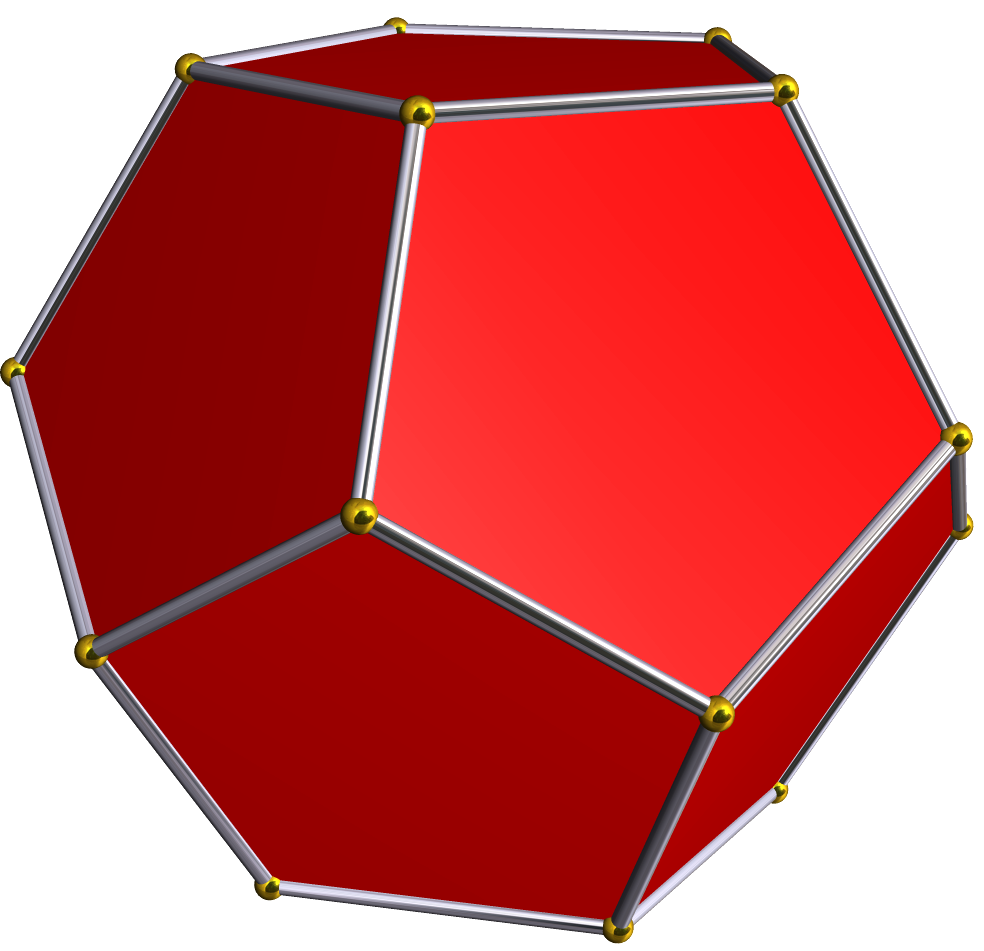
\includegraphics[scale=0.2]{Dodecahedron.png}

{\tiny A picture of a dodecahedron from Wikipedia}
\end{center}


Let $G$ be the group of isometries of the dodecahedron that preserve orientation:
$$G \colonequals \{\alpha : \R^3 \to \R^3 \mid \text{$\alpha$ is an isometry, $\alpha$ preserves orientation, and } \alpha(X) = X\}.$$
This is a subgroup of the group of all bijections from $\R^3$ to $\R^3$. Though not obvious, every element of $G$ is given as rotation about a line of symmetry. There are three kinds of such lines: those joining midpoints of opposite face, those joining midpoints of opposite edges, and those joining opposite vertices.  To count the number of elements of $G$ informally, think about an isometry as picking up a dodecaedron that was lying on a table and replacing it in the same location.  To do this, one must first pick one of the twelve faces to place on the table, and, for each possible face, there are five ways to orient it. Thus 
$$|G|=12 \cdot 5 = 60.$$

Let us use \hyperref[lois]{LOIS} to do this more formally. Note that $G$ act on the collection $S$ of the $12$ faces of $X$. This action is transitive since it is possibly to move one face to any other via an appropriate rotation. So, the one and only orbit has length $12$. Letting $F$ be any one of the faces, the orientation preserving isometries of $X$ that map $F$ to itself are just the orientation-preserving elements of $D_{5}$, of which there are $5$. Indeed, these correspond to the five rotations of $X$ by $\frac{2 \pi n j}{5}$ radians for $j =0,1,2,4$ about the axis of symmetry passing through the midpoint of $F$ and the midpoint of the opposite face.
  Applying the \hyperref[Orbit-Stabilizer Theorem]{Orbit-Stabilizer Theorem} gives
$$|G|=|\Orb_G(F)|\cdot |\Stab_G(F)]=12 \cdot 5=60.$$
\end{example}





\section{The class equation}

The main goal of this subsection is to apply the Orbit-Stabilizer Formula to the action of $G$ on itself by conjugation. 
Let $G$ be a group. As we saw before, $G$ acts on $S = G$ by conjugation: the action is defined by $g \cdot x=gxg^{-1}$.

\begin{definition}\index{conjugate elements}
Let $G$ be a group. Two elements $g,g' \in G$ are {\bf conjugate} if there exists $h \in G$ such that 
$$g' = hgh^{-1}.$$
Equivalently, $g$ and $g'$ are conjugate if they are in the same orbit of the conjugation action. The \df{conjugacy class} of an element $g \in G$ is 
$$[g]_c \colonequals \{hgh^{-1} \mid h \in G\}.$$ 
Equivalently, the conjugacy class of $g$ is the orbit of $g$ under the conjugation action. 
\end{definition}


\begin{remark}
	Let $G$ be any group. Then $geg^{-1} = e$ for all $g \in G$, and thus $[e]_c=e = \{ e \}$.
\end{remark}

Let us study the conjugacy classes of $S_n$. You proved in a problem set that two cycles in $S_n$ are conjugate if and only if they have the same length:

\begin{lemma}\label{lemma conjugates cycles} 
For any $\sigma \in S_n$ and distinct integers $i_1, \dots, i_p$, we have
$$\sigma (i_1 \, i_2 \, \cdots i_p) \sigma^{-1} = (\sigma(i_1) \, \cdots \, \sigma(i_p)).$$
\end{lemma}

Note that the right-hand cycle is a cycle since $\sigma$ is injective. This generalizes to the following:

\begin{theorem}\label{conjugates S_n}
Two elements of $S_n$ are conjugate if and only if they have the same cycle type. 
\end{theorem}

%To prove this, we need a lemma, which you proved in a problem set:


\begin{proof}
Consider two conjugate elements of $S_n$, say $\alpha$ and $\beta = \s \alpha \s^{-1}$. By \Cref{every permutation is a product of disjoint cycles}, we may write $\alpha$ as a product of disjoint cycles $\alpha = \alpha_1 \cdots \alpha_m$. Then 
$$\beta = \s \alpha \s^{-1} = (\s \alpha_1 \s^{-1})  \cdots (\s \alpha_m \s^{-1}).$$ 
Since $\alpha_1, \ldots, \alpha_m$ are disjoint cycles, then by \Cref{lemma conjugates cycles} the elements $(\s \alpha_1 \s^{-1}),   \cdots, (\s \alpha_m \s^{-1})$ are also disjoint cycles, and $\s \alpha_i \s^{-1}$ has the same length as $\alpha_i$.
We conclude that $\alpha$ and $\beta$ must have the same cycle type.

Conversely, consider two elements $\alpha$ and $\beta$ with the same cycle type. More precisely, assume $\alpha = \alpha_1 \cdots \alpha_k$ and $\beta = \beta_1 \cdots \beta_k$ are decompositions into disjoint cycles and that $\alpha_i, \beta_i$ both have length $p_i \geqslant 2$ for each $i$. We need to prove that $\alpha$ and $\beta$ are conjugate. Let us start with the case $k = 1$. Given two cycles of the same length,
$$\alpha = (i_1 \, \dots \, i_p) \quad \text{ and } \quad \beta = (j_1 \, \dots \, j_p).$$
By \Cref{lemma conjugates cycles}, any permutation $\s$ such that $\s(i_m) = j_m$ for all $1 \leqslant m \leqslant p$ must satisfy $\s \alpha \s^{-1} = \beta$. 


Note that such $\s$ has no restrictions on what it does to the set $\{1, \dots, n\} \setminus \{i_1 \, \dots \, i_p\}$: it can map $\{1, \dots, n\} \setminus \{i_1 \, \dots \, i_p\}$ bijectively to $\{1, \dots, \} \setminus \{j_1 \, \dots \, j_p\}$ in any way possible. From this observation, the general case follows: since the cycles are disjoint, we can find a single permutation $\s$ such that $\s \alpha_i \s^{-1} = \beta_i$ for all $i$.
\end{proof}

We can now classify all the conjugacy classes in $S_n$ based on their cycle type.

\begin{example}
Given \Cref{conjugates S_n}, we can now write a complete list of the conjugacy classes of $S_4$:
\begin{enumerate}[itemsep=-0.1em]
\item The conjugacy class of the identity $\{e\}$. 
\item The conjugacy class of $(12)$, which is the set of all two cycles and has ${4 \choose 2} = 6$ elements.
\item The conjugacy class of $(123)$, which is the set of all three cycles and has $4 \cdot 2 = 8$ elements.
\item The conjugacy class of $(1234)$, which is the set of all four cycles and has $3! = 6$ elements.
\item The conjugacy class of $(12)(34)$, which is the set of all products of two disjoint $2$-cycles and has $3$ elements.
\end{enumerate}
We can check our work by recalling that the conjugacy classes partition $S_4$, and indeed we counted $24$ elements.
\end{example}



\begin{example}
Given \Cref{conjugates S_n}, we can now write a complete list of the conjugacy classes of $S_5$:
\begin{enumerate}[itemsep=-0.1em]
\item The conjugacy class of the identity $\{e\}$. 
\item The conjugacy class of $(12)$, which is the set of all $2$-cycles and has ${5 \choose 2} = 10$ elements.
\item The conjugacy class of $(123)$, containing all $3$-cycles, of size $2! \cdot {5 \choose 3} = 20$ elements.
\item The conjugacy class of $(1234)$, containing all $4$-cycles, of size $5 \cdot 3! = 30$ elements.
\item The conjugacy class of $(12345)$, which is the set of all $5$-cycles, and has $4! = 24$ elements.
\item The conjugacy class of $(12)(34)$, which is the set of all products of two disjoint $2$-cycles and has $5 \cdot  3= 15$ elements.
\item The conjugacy class of $(12)(345)$, which is the set of all products of a $2$-cycle by a $3$-cycle, and has ${5 \choose 2} \cdot 2! = 20$ elements.
\end{enumerate}
We can check our work by noting that indeed
$$1 + 10 + 20 + 30 + 24 + 15 + 20 = 120 = 5!.$$
\end{example}


\begin{remark}
	For any nontrivial group $G$, since $[e]_c = \{ e \}$ and the conjugacy classes partition $G$, then $[g]_c \neq G$ for all $g \in G$.
\end{remark}


%\begin{example}
%One thing we get from the previous example and lemma is a very short list of all possible sizes of normal subgroups of $S_4$. Here's why:
%
%An important, general observation is that, any group $G$ and $N \nsg G$, since $gNg^{-1} = N$ for all
%$g$, it follows that $N$ is necessarily a union of conjugacy classes. In other words, the action of $G$ on itself by conjugation restricts to an action on $N$
%since $N$ is normal, and thus $N$ is a union of orbits of this action. Moreover, if $G$ is finite then,
%by Lagrange, $|N| \mid |G|$. Finally, $N$ certainly contains $e$. Putting these facts together we get than $|N|$ must both divide $|G|$ and be a sum of
%cardinalities of conjugacy classes, including the class $\{e\}$.
%
%For example, if  $N \nsg S_4$, then $|N| \mid 24$ and $|N|$ must equal $1$ plus the sum of some sub-list of 
%$6, 8, 6, 3$. The only possibilities are
%$$
%1, 1 + 3, 1 + 3 + 8, \and 1 + 6 + 8 + 6 + 3
%$$
%The first and last represent the boring normal subgroups: $\{e\}$ and $G$. $1 + 3$ also represents a normal subgroup, which consists of all the products of all product of two disjoint two cycles and the identity:
%$$V=\{e, (1 2)(3 4), (1 3)(2 4), (1 4)(2 3)\}.$$ The last one exists too and it is $A_4$.
%\end{example}
%
%
%


\begin{definition}\index{centralizer}\index{$C_G(a)$}
Let $G$ be a group and $a\in G$. The \df{centralizer} of $a$ is the set of elements of $G$ that commute with $a$: 
$$C_G(a) \colonequals \{x \in G \mid xa=ax\}.$$
More generally, given a subset $S \subseteq G$, the \df{centralizer} of $S$ is the set
$$C_G(S) \colonequals \{x \in G \mid xs=sx \textrm{ for all } s \in S \}$$
\end{definition}


\begin{definition}\index{normalizer}\index{$N_G(a)$}
Let $G$ be a group and consider a subset $S \subseteq G$. The \df{normalizer} of $S$ is the set 
$$N_G(S) \colonequals \{g \in G \mid gSg^{-1}=S\}.$$
\end{definition}


\begin{exercise}
Let $G$ be a group and $S \subseteq G$. 
Prove that the centralizer and the normalizer of $S$ are subgroups of $G$.
\end{exercise}


\begin{lemma}
	Let $S \subseteq G$ be any subset of a group $G$. Then $C_G(S) \subseteq N_G(S)$.
\end{lemma}

\begin{proof}
	Let $G$ be a group and $S \subseteq G$. If $x \in C_G(S)$, then for all $s \in S$ we have
	$$xs=sx \implies xsx^{-1} = s \in S \textrm{ and } x^{-1}sx = s.$$
	Thus $xSx^{-1} \subseteq S$ and $x^{-1}Sx \subseteq S$.
	Now for any $s \in S$ we have $x^{-1}sx \in S$ and $s$ can be written as 
	$$s = x(x^{-1}sx)x^{-1} \in xSx^{-1}.$$ 
	This shows that $S \subseteq xSx^{-1}$. Thus $xSx^{-1} = S$, and therefore $x \in N_G(S)$.
\end{proof}

\begin{remark}
	If $G$ is an abelian group, then for any $a \in G$ we have $C_G(a) = G = N_G(a)$.
\end{remark}


\begin{exercise}\label{centralizer and normalizer in subgroup}
	Let $H$ be a subgroup of a group $G$, and $S$ a subset of $H$. Then 
	$$C_{H}(S) = C_G(S) \cap H \quad \textrm{and} \quad N_{H}(S) = N_G(S) \cap H.$$
\end{exercise}




\begin{exercise}
Let $G$ be a group and let $H$ be a subgroup of $G$. 
Show that $N_G(H)/C_G(H)$ is isomorphic to a subgroup of the automorphism group $\Aut(H)$ of $H$.
\end{exercise}


\begin{exercise}
Let $G$ be a group and $H$ a subgroup of $G$. Prove that if $H$ is normal in $G$, then so is $C_G(H)$, and that $G/C_G(H)$ is isomorphic to a subgroup of the automorphism group of $H$.
\end{exercise}

%
%\begin{exercise}\label{conjugacy class}
%Let $G$ be a group. 
%\begin{enumerate}
%\item Consider the action of $G$ on $G$ by conjugation, where $g \cdot h = ghg^{-1}$. For all $g \in G$, 
%$$\Orb_G(g) = [g]_c \quad \textrm{and} \quad \Stab_G(g)=C_G(G) \quad \textrm{and} \quad |[g]_c| = [G : C_G(g)].$$
%\item Consider the action of $G$ on the power set of $G$, $P(G)=\{S\mid S\subseteq G\}$, by conjugation, meaning $g \cdot S = gSg^{-1}$. For all $S \in P(G)$, 
%$$\Stab_G(S)=N_G(S) \quad \textrm{and} \quad |\Orb_G(S)| = [G : N_G(S)].$$
%\end{enumerate}
%\end{exercise}
%

\begin{lemma}\label{conjugacy class}
	Let $G$ be a group. Consider the action of $G$ on $G$ by conjugation, where $g \cdot h = ghg^{-1}$. For all $g \in G$, 
$$\Orb_G(g) = [g]_c \quad \textrm{and} \quad \Stab_G(g)=C_G(g) \quad \textrm{and} \quad |[g]_c| = [G : C_G(g)].$$
\end{lemma}


\begin{proof}
	The first statement is the definition of the conjugacy class of $g$: $\Orb_G(g) = [g]_c$. 	
	Moreover, by simply following the definitions we see that
	$$h \in \Stab_G(g) \iff h \cdot g = g \iff hgh^{-1} = g \iff hg = gh \iff h \in C_G(G).$$
	Thus, $\Stab_G(g)=C_G(G)$, and by the \hyperref[Orbit-Stabilizer Theorem]{Orbit-Stabilizer Theorem},
	$$|[g]_c| = |\Orb_G(g)| = [G : C_G(g)].\qedhere$$
\end{proof}


\begin{exercise}\label{conjugacy class exercise}
Let $G$ be a group. Consider the action of $G$ on the power set 
$$P(G)=\{S\mid S\subseteq G\}$$ 
of $G$ by conjugation, meaning $g \cdot S = gSg^{-1}$. For all $S \in P(G)$, 
$$\Stab_G(S)=N_G(S) \quad \textrm{and} \quad |\Orb_G(S)| = [G : N_G(S)].$$
\end{exercise}


\begin{corollary}
For a finite group $G$, the size of any conjugacy class divides $|G|$.	
\end{corollary}

\begin{proof}
Let $g \in G$. By \Cref{conjugacy class}, the order of the conjugacy class of $g$ is the index of the centralizer: 
$$|[g]_c| = [G : C_G(g)]$$ 
By \hyperref[Lagrange]{Lagrange's Theorem}, the index of any subgroup must divide $|G|$, and thus in particular $|[g]_c|$ divides $|G|$.
\end{proof}


We will take the \hyperref[Orbit Equation]{Orbit Equation} and apply it to the special case of the conjugation action. In order to do that, all that remains is to identify the fixed points of the action.


\begin{lemma}\label{fixed points conjugation are central}
	Let $G$ be a group acting on itself by conjugation. An element $g \in G$ is a fixed point of the conjugation action if and only $g \in \Zc(G)$.
\end{lemma}

\begin{proof}
$(\Leftarrow)$ Suppose that $g \in \Zc(G)$. Then for all $h \in G$, $g$ commutes with $h$, and thus
$$hgh^{-1} = (hg)h^{-1} = g(hh^{-1}) = g.$$
Thus $g$ is conjugate to only itself, meaning it is a fixed point for the conjugation action. 

$(\Rightarrow)$ Conversely, suppose that $g$ is a fixed point for the conjugation action. Then for all $h \in G$,
$$hgh^{-1} = h \cdot g = g \implies hg=gh.$$
Thus $g \in \Zc(G)$.	
\end{proof}


We can now write the \hyperref[Orbit Equation]{Orbit Equation} for the conjugation action; this turns out to be a very useful formula.

\begin{theorem}[The Class Equation]\label{class equation}
Let $G$ be a finite group. For each conjugacy class of size greater than $1$, pick a unique representative, and let $g_1,\ldots g_r \in G$ be the list of all the chosen representatives. Then 
$$|G| = |\Zc(G)| + \sum_i^r |G : C_G(g_i)|.$$
\end{theorem}

\begin{proof}
 By \Cref{fixed points conjugation are central}, the elements of $\Zc(G)$ are precisely the fixed points of the conjugation action. In particular, $|\Zc(G)|$ counts the number of orbits that have only one element. Because the orbits of the conjugation action partition $G$, and the conjugacy classes are the orbits, then as noted in \Cref{Orbit Equation}
$$|G| = |\Zc(G)| + \sum_i^r [g_i]_c.$$
By \hyperref[lois]{LOIS}, the index of the stabilizer is the order of the conjugacy class. Thus for each $g_i$ as in the statement we have 
$$[g_i]_c = [G: C_G(g_i)].$$ 
The class equation follows from substituting this into the equation above:
$$|G| = |\Zc(G)| + \sum_i^r |G : C_G(g_i)|.\qedhere$$
\end{proof}



\begin{remark}
	The \hyperref[Class Equation]{class equation} is not very interesting if $G$ is abelian, since there is only one term on the right hand side: $|\Zc(G)|$.
\end{remark}

But when $G$ is nonabelian, the class equation can lead us to discover some very interesting facts, despite its simplicity.

\begin{exercise}
Prove that if $G$ is a nonabelian group of order $21$, then there is only one possible class equation for $G$, meaning that the numbers appearing in the class equation are uniquely determined up to permutation.
\end{exercise}



%%Eg Qualunl
\begin{corollary}
If $p$ is a prime number and $G$ is a finite group of order $p^m$ for some $m > 0$, then $\Zc(G)$ is not the trivial group.
\end{corollary}

\begin{proof}
Let $g_1,\ldots g_r \in G$ be a list of unique representatives of all of the conjugacy classes of $G$ of size greater than 1, as in the \hyperref[Class Equation]{class equation}. By construction, each $g_i$ is not a fixed point of the action, and thus $\Stab_G(g_i) \neq G$. By \Cref{conjugacy class}, $C_G(g_i) = \Stab_G(g_i)$, so $C_G(g_i) \neq G$. In particular, $[G:C_G(g_i)]\neq 1$. Since $1\neq [G:C_G(g_i)]$ and $[G:C_G(g_i)]$ divides $|G|=p^m$, we conclude that $p$ divides $[G:C_G(g_i)]$ for each $i$. From the \hyperref[Class Equation]{class equation}, we can now conclude that $p$ divides $|\Zc(G)|$, and in particular $|\Zc(G)|\neq 1$.
\end{proof}





\begin{exercise}
Let $p$ be prime and let $G$ be a group of order $p^m$ for some $m \geqslant 1$. Show that if $N$ is a nontrivial normal subgroup of $G$, then $N \cap Z(G) \ne \{e\}$. In fact, show that $|N \cap Z(G)| = p^j$ for some $j \geqslant 1$. 
\end{exercise}



\begin{lemma}\label{conjugation descends to normal subgroups}
Let $G$ be a group and $N\norm G$. The conjugation action of $G$ on itself induces an action by conjugation of $G$ on $N$. In particular, $N$ is the disjoint union of some of the conjugacy classes in $G$.
\end{lemma}


\begin{proof}
Define the conjugation action of $G$ on $N$ by $g\cdot n=gng^{-1}$ for all $g\in G$ and $n\in N$. Since $N\norm G$, this always gives us back an element of $N$, and thus the action is well-defined. We can think of this action as a restriction of the action of $G$ on itself by conjugation, and thus the two properties in the definition of an action hold for the action of $G$ by conjugation on $N$. Therefore, this is indeed an action. The orbits of elements $n\in N$ under this action are the conjugacy classes $[n]_c$, and we have just shown that for all $n \in N$, $[n]_c \subseteq N$. But every element in $N$ belongs to some conjugacy class, thus the conjugacy classes of the elements of $N$ partition $N$.
\end{proof}


\begin{remark}\label{remark conjugation descending}	
\Cref{conjugation descends to normal subgroups} says that the orbits of the conjugation action of $G$ on a normal subgroup $N$ are just the orbits of the conjugation action of $G$ on itself that contain elements of $N$ (and must thus be completely contained in $N$). In contrast, if $N$ is a normal subgroup of $G$, we can also consider the conjugation action of $N$ on itself. If $a$ and $b$ are elements of $N$ that are conjugate for the $N$-conjugation, then they must also be conjugate for the $G$-conjugation action, using the same element $n \in N$ such that $a =nbn^{-1}$. However, if $a$ and $b$ are conjugate for the $G$-conjugation, they might not necessarily be conjugate for the $N$-action, as all the elements $g \in G$ such that $a = gbg^{-1}$ could very well all be in $G \setminus N$.
\end{remark}

We will see examples of this in the next section, where we will study the special case of the alternating group.

%
%\begin{proof}
%	The containment $C_{H}(S) \subseteq C_G(S) \cap H$ is immediate by definition. On the other hand, if $c \in C_G(S) \cap H$, then 
%\end{proof}

\newpage

\section{The alternating group}


%Let us analyze the conjugacy classes of $A_n$. 
Since $A_n \leq S_n$, we know that {\em if} two elements of $A_n$ are conjugate, {\em then} they have the same cycle type, as they are also conjugate elements of $S_n$, and thus we can apply \Cref{conjugates S_n}. But as noted in \Cref{remark conjugation descending}, there is no reason for the converse to hold: given $\alpha, \beta \in A_n$ of the same cycle type, the elements $\sigma \in S_n$ such that $\sigma \alpha \sigma^{-1} = \beta$ might all belong to $S_n \setminus A_n$. Indeed, we will see that this does happen in some cases.


\begin{example}
The two permutations $(123)$ and $(132)$ are not conjugates in $A_3$, despite having the same cycle type and thus being conjugate in $S_3$ by \Cref{conjugates S_n}. One can check this easily, for example, by conjugating $(123)$ by the $3$ elements in $A_3$.
\end{example}

%
%\begin{example}[Conjugacy classes of $A_5$] 
%Let us analyze the conjugacy classes of $A_5$. 
%
%Since $A_5 \leq S_5$, we know that {\em if} two elements of $A_5$ are conjugate, {\em then} they have the same cycle type, as they are also conjugate elements of $S_5$, and thus we can apply \Cref{conjugates S_n}. But there is no reason for the converse to hold: given $\alpha, \beta \in A_5$ of the same cycle type, the elements $\sigma \in S_5$ such that $\sigma \alpha \sigma^{-1} = \beta$ might all belong to $S_5 \setminus A_5$. Indeed, this does happen in some cases.
%
%
%
%
%The possible cycle types of elements of $A_5$ are
%\begin{enumerate}
%\item Five cycles: there are $4! = 24$ such elements.
%\item Three cycles: there are ${5 \choose 3} 2 =   20$ such elements.
%\item Products of two disjoint transpositions: there are $5 \cdot 3 = 15$ such elements.
%\item The identity $\{e\}$.
%\end{enumerate}
%
%Let us start with five cycles. Let $\s = (1 \, 2 \, 3 \, 4 \, 5)$.  
%We have by Theorem \ref{thm:conjclass} (a) that
%$$
%C_{C_5}(\s) = \frac{C_5}{\left|\text{ conjugacy class of }\s \text{ in }S_5\right|}=\frac{5!}{4!}=5.$$
%This yields  that the centralizer of $\s$ {\em in $S_5$} is
%$$
%C_{S_5}(\s) = \{e, \s, \s^2, \s^3, \s^4\},
%$$
%since the five listed permutations do commute with $\s$ and there can be no more elements in $C_{S_5}(\s) $ because of cardinality reasons.
%Moreover, it is obvious from the definitions that
%$$
%C_{A_5}(\s) = C_{S_5}(\s) \cap A_5
%$$
%and so we conclude that 
%$$
%C_{A_5}(\s) = \{e, \s, \s^2, \s^3, \s^4\}
%$$
%too. Thus, by LOIS, 
%$$
%\text{ the size of the conjugacy class of $\s$ in $A_5$} = [A_5: C_{A_5}(\s)] = 60/5 = 12.
%$$
%That is, $\s$ is only conjugate in $A_5$  to half of the five cycles. 
%
%If we pick a five cycle $\sigma'$ that is not conjugate in $A_5$ to $\sigma$, the same reasoning shows that $\sigma'$ is conjugate to exactly $12$ elements, which must be exactly
%the other $12$ five cycles. It is not hard to see that in fact
%$(1 \, 2 \, 3 \, 4 \, 5)$ and $(2 \, 1 \, 3 \, 4 \, 5)$ are not conjugate. In a bit more detail, they {\em are} conjugate {\em in $S_5$} via the element $(1 \,2)$. From this one sees that the only elements $\a$ in $S_5$ such that
%$$
%\a (1 \, 2 \, 3 \, 4 \, 5) \a^{-1} = (2 \, 1 \, 3 \, 4 \, 5)
%$$ 
%holds are members of the coset $C_{S_5}(\s) \cdot (1 \, 2)$, which contains no elements of $A_5$.)
%
%
%So far we know the following about the conjugacy classes of $A_5$:
%\begin{enumerate}
%\item the conjugacy class of $(1 \, 2 \, 3 \, 4 \, 5)$ has $12$ elements,
%\item the conjugacy class of $(2 \, 1 \, 3 \, 4 \, 5)$ has $12$ elements, and this class is distinct from the previous one, and
%\item the collection of all three cycles, of which there are $20$, forms one or more conjugacy classes,
%\item the collection of all products of two disjoint transpositions, of which there are $15$, forms one or more conjugacy classes.
%\item $\{e\}$ is a conjugacy class,
%\end{enumerate}
%
%Given two three cycles $(a \, b \, c)$ and $(d \, e \, f)$, there is a $\s \in S_5$ such that
%$$
%\s (a \, b \, c) \s^{-1}  = (d \, e \, f).
%$$
%If $\s$ is not in $A_5$, then let $x,y$ be the two elements of $\{1, \dots, 5\} \setminus \{a,b,c\}$. Then we have
%$$
%(\s \cdot (x \, y)) (a \, b \, c) (\s \cdot (x \, y))^{-1}  = (d \, e \, f).
%$$
%and $\s \cdot (x \, y) \in A_5$. 
%
%
%To figure out what's going on the in last case, set $\alpha = (1 \, 2)(3 \, 4)$. Because the cardinality of the conjugacy class of $\alpha$ in $S_5$ is 15 (it consists of all the products of two disjoint two-cycles) we get
%$$
%15=|[\alpha]_{c\text{ in } S_5}|=[S_5: C_{S_5}(\alpha)]=\frac{120}{\left|C_{S_5}(\alpha)\right|}\Rightarrow \left|C_{S_5}(\alpha)\right| = 8.
%$$
%Since
%$$
%C_{A_5}(\alpha) = C_{S_5}(\alpha) \cap A_5,
%$$
%it follows that $\# C_{A_5}(\alpha)$ must divide both $8$ and $60$, and so must be one of $1, 2$ or $4$. Since $\alpha$ commutes with
%$e$, $\alpha$, $(1 \, 3)(2 \, 4)$ and $(1 \, 4)(2 \, 3)$ and  each of these belongs to $A_5$, we must have 
%$\# C_{A_5}(\a) = 4$. It follows that $\a$ is conjugate to $60/4 = 15$ elements -- i.e., $\a$ must be conjugate in $A_5$ to all elements of its cycle type. 
%
%
%
%We conclude that  the conjugacy classes of $A_5$ are given by the following list:
%\begin{enumerate}
%\item the conjugacy class of $(1 \, 2 \, 3 \, 4 \, 5)$ has $12$ elements,
%\item the conjugacy class of $(2 \, 1 \, 3 \, 4 \, 5)$ has $12$ elements, and this class is distinct from the previous one, 
%\item the collection of all three cycles, of which there are $20$, forms a conjugacy class, 
%\item the collection of all products of two disjoint transpositions, of which there are $15$, forms one conjugacy class, and
%\item $\{e\}$ is a conjugacy class.
%\end{enumerate}
%\end{example}


\begin{lemma}\label{cycle types in An}
Let $\sigma$ be an $m$-cycle in $S_n$. Then
$$\sigma \in A_n \iff m \textrm{ is odd}.$$
\end{lemma}


\begin{proof}
Recall that by \Cref{exercise formula for rewriting cycles in terms of 1},
$$(i_1 \, i_2 \, \cdots \, i_m) = (i_1 \, i_m) (i_1 \, i_{m-1}) (i_1 \, i_3) (i_1 \, i_2)$$
is a product of $m-1$ transpositions.
Thus $\sigma$ is even if and only if $m-1$ is even.
\end{proof}


\begin{lemma}[Conjugacy classes of $A_5$]\label{conjugacy classes of A5}
The conjugacy classes of $A_5$ are given by the following list:
\begin{enumerate}[itemsep=-0.1em]
\item The singleton $\{e\}$ is a conjugacy class.
\item The conjugacy class of $(1 \, 2 \, 3 \, 4 \, 5)$ in $A_5$ has $12$ elements.
\item The conjugacy class of $(2 \, 1 \, 3 \, 4 \, 5)$ in $A_5$ has $12$ elements, and it is disjoint from the conjugacy class of $(1 \, 2 \, 3 \, 4 \, 5)$. 
\item The collection of all three cycles, of which there are $20$, forms a conjugacy class in $A_5$.
\item The collection of all products of two disjoint transpositions, of which there are $15$, forms one conjugacy class in $A_5$.
\end{enumerate}
\end{lemma}


As a reality check, note that $12 + 12 + 20 + 15 + 1 = 60 = |A_5|$.


\begin{proof}
By \Cref{cycle types in An}, the cycle types of elements of $A_5$ are
\begin{itemize}[itemsep=-0.1em]
\item five cycles, of which there are $4! = 24$, 
\item three cycles, of which there are ${5 \choose 3} 2 =   20$,
\item products of two disjoint transpositions, of which there are $5 \cdot 3 = 15$, and
\item the unique $1$-cycle e, and indeed $[e]_c = \{e\}$.
\end{itemize}

By \Cref{conjugates S_n}, we know that two permutations are conjugate in $S_5$ if and only if they have the same cycle type. It follows that the conjugacy classes in $A_5$ form a subset of the cycles types.
The statement we are trying to prove asserts that the set of five cycles breaks apart into two conjugacy classes in $A_5$, whereas in all the other cases, the conjugacy classes remain whole. 



{\bf Claim}: Fix a $5$-cycle $\sigma$. The conjugacy class of $\sigma$ in $A_5$ has $12$ elements.


\vspace{0.5em}

\noindent
By \hyperref[Lagrange]{Lagrange's Theorem},
$$|C_{S_5}(\sigma)| = \frac{|S_5|}{[S_5 : C_{S_5}(\sigma)]}.$$
By \Cref{conjugacy class}, 
$$[S_5 : C_{S_5}(\sigma)] = |[\sigma]_c|.$$
By \Cref{conjugates S_n}, this is the number of $5$-cycles in $S_5$, which is $4!$.
Thus
$$|C_{S_5}(\sigma)| = \frac{5!}{4!} = 5.$$
Since every power of $\sigma$ commutes with $\sigma$, and there are $5$ such elements, we conclude that
$$C_{S_5}(\sigma) = \{e, \sigma, \sigma^2, \sigma^3, \sigma^4\}.$$
But these are all in $A_5$, and thus by \Cref{centralizer and normalizer in subgroup} we conclude that
$$C_{A_5}(\sigma) = C_{S_5}(\sigma) \cap A_5 = \{e, \sigma, \sigma^2, \sigma^3, \s^4\}.$$
By \hyperref[lois]{LOIS}, \Cref{conjugacy class}, and \hyperref[Lagrange]{Lagrange's Theorem}, 
$$\text{ the size of the conjugacy class of $\sigma$ in $A_5$} = [A_5: C_{A_5}(\sigma)] = \frac{|A_5|}{|C_{A_5}(\sigma)|} = \frac{60}{5} = 12.$$
This proves the claim.


\

We have now shown that the conjugacy class of each $5$-cycle has $12$ elements, and all twenty-four $5$-cycles are in $A_5$. Thus there are two conjugacy classes of $5$-cycles in $A_5$.
This shows that $\sigma$ is only conjugate in $A_5$ to half of the five cycles. 
If we pick two $5$-cycles $\sigma$ and $\tau$ that are not conjugate in $A_5$, then $\tau$ is conjugate to exactly $12$ elements, which must be exactly the other $5$-cycles that $\sigma$ is not conjugate to. 


One can see that in fact $(1 \, 2 \, 3 \, 4 \, 5)$ and $(2 \, 1 \, 3 \, 4 \, 5)$ are not conjugate.
While they {\em are} conjugate {\em in $S_5$}, it is via the element $(1 \,2)$, which is {\em not} in $A_5$.
Suppose that $\alpha \in S_5$ is such that
$$\alpha (2 \, 1 \, 3 \, 4 \, 5) \alpha^{-1} = (1 \, 2 \, 3 \, 4 \, 5).$$
Note that $\tau = \alpha (1 \, 2)$ satisfies
$$\begin{aligned}
\tau (1 \, 2 \, 3 \, 4 \, 5) & =  \alpha (1 \, 2) (1 \, 2 \, 3 \, 4 \, 5) \\
& = \alpha (2 \, 1 \, 3 \, 4 \, 5) \\
& = (2 \, 1 \, 3 \, 4 \, 5) \alpha \\
& = (1 \, 2 \, 3 \, 4 \, 5) (1 \, 2) \alpha \\
& = (1 \, 2 \, 3 \, 4 \, 5) \tau.
\end{aligned}$$
Thus $\alpha (1 \, 2) \in C_{S_5}(1 \, 2 \, 3 \, 4 \, 5)$, or equivalently, 
$$\alpha \in (1 \, 2) \cdot C_{S_5}(2 \, 1 \, 3 \, 4 \, 5).$$
But note that we just proved that every element in $C_{S_5}(2 \, 1 \, 3 \, 4 \, 5)$ is in $A_5$, and thus even; this shows that every element in the coset 
$$(1 \, 2) \cdot C_{S_5}(2 \, 1 \, 3 \, 4 \, 5)$$
is odd (as we multiplied by \emph{one} transposition), and thus there are no such $\alpha$ in $A_5$.
%In fact, the only elements $\alpha$ in $S_5$ such that
%$$\alpha (1 \, 2 \, 3 \, 4 \, 5) \alpha^{-1} = (2 \, 1 \, 3 \, 4 \, 5)$$ 
%holds are members of the coset $C_{S_5}(1 \, 2 \, 3 \, 4 \, 5) \cdot (1 \, 2)$, which contains no elements of $A_5$.
This proves (1) and (2).



\vspace{1.5em}

{\bf Claim}: All $20$ three cycles are conjugate in $A_5$.

\vspace{0.5em}

Given two three cycles $(a \, b \, c)$ and $(d \, e \, f)$ in $S_5$, we already know that they are both in $A_5$ and that there is a $\sigma \in S_5$ such that
$$
\sigma (a \, b \, c) \sigma^{-1}  = (d \, e \, f).
$$
If $\sigma \notin A_5$, let $\{1, \dots, 5\} \setminus \{a,b,c\} = \{ x, y\}$. Then $\sigma$ is a product of an odd number of transpositions, so $\sigma \cdot (x \, y) \in A_5$. Moreover, since $(x \, y)$ and $(a \, b \, c)$ are disjoint cycles, then by \Cref{disjoint cycles commute} they must commute, so that
$$(x \, y) (a \, b \, c) (x \, y))^{-1} = (a \, b \, c).$$
Therefore,
$$(\sigma \cdot (x \, y)) (a \, b \, c) (\sigma \cdot (x \, y))^{-1}  = (d \, e \, f),$$
so $(a \, b \, c)$ and $(d \, e \, f)$ are still conjugate in $S_5$.
This proves the claim.

\vspace{1.5em}

{\bf Claim}: All products of two disjoint transpositions are conjugate in $A_5$.

\vspace{0.5em}


Set $\alpha = (1 \, 2)(3 \, 4)$. The conjugacy class of $\alpha$ in $S_5$ consists of all the products of two disjoint two-cycles, and there are $15$ such elements. By \hyperref[lois]{LOIS} and \Cref{conjugacy class},
$$15 = |\text{ the conjugacy class of $\alpha$ in $S_5$ }|
= [S_5: C_{S_5}(\alpha)]=\frac{120}{\left|C_{S_5}(\alpha)\right|}.$$
Thus
$$\left|C_{S_5}(\alpha)\right| = \frac{120}{15} = 8.$$
Since $\alpha$ commutes with $e$, $\alpha$, $(1 \, 3)(2 \, 4)$ and $(1 \, 4)(2 \, 3)$ and each of these belongs to $A_5$, we must have $|C_{A_5}(\alpha)| \geqslant 4$.
Since, by \Cref{centralizer and normalizer in subgroup},
$$C_{A_5}(\alpha) = C_{S_5}(\alpha) \cap A_5,$$
it follows that $|C_{A_5}(\alpha)|$ must divide both $8$ and $60$, and so must be $1$, $2$ or $4$.  
We conclude that $|C_{A_5}(\alpha)| = 4$. Thus $\alpha$ is conjugate in $A_5$ to $60/4 = 15$ elements. Since there are $15$ products of disjoint two-cycles, they must all be conjugate to $\alpha$, and thus the conjugacy class of $\alpha$ in $A_5$ is still the set of all $2$-cycles.
\end{proof}


\

 Now that we have completely calculated all the conjugacy classes of $A_5$, our hard work will pay off: we can now prove a very important result in group theory.




\begin{definition}\index{simple group}
	A nontrivial group $G$ is {\bf simple} if it has no proper nontrivial normal subgroups.
\end{definition}


\begin{exercise}
	Let $p$ be prime. Show that $\Z/p$ is a simple group.
\end{exercise}


\vspace{0.5em}


\begin{theorem}\label{A5 is simple}
The group $A_5$ is a simple group.
\end{theorem}

\begin{proof} 
Suppose $N \norm A_5$. By \hyperref[Lagrange]{Lagrange's Theorem}, $|N|$ divides 
$$|A_5| = \frac{5!}{2} = 60.$$ 
By \Cref{conjugacy classes of A5}, $A_5$ has only four nontrivial conjugacy classes, and they have order $12$, $12$, $15$, and $20$. By \Cref{conjugation descends to normal subgroups}, $|N|$ is a union of conjugacy classes of $A_5$.
Thus
$$|N| = 1 + \text{ the sum of a sublist of the list $20, 12, 12, 15$}.$$
By checking the relatively small number of cases we see that $|N| = 1$ or $|N| = 60$ are the only possibilities, as the remaining options do not divide $60$.
\end{proof}



In fact, $A_n$ is simple for all $n \geqslant 5$, but we will not prove this. In contrast, $A_4$ is not simple:



\begin{example}
	The alternating group $A_3$ is simple and abelian since it has order $3$. 
\end{example}

Both $A_1$ and $A_2$ are the trivial group. 


\begin{exercise}
	Consider the subset of $A_4$ given by
	$$V = \{e,  (1 \, 2)(3 \, 4),  (1 \, 3)(2 \, 4),  (1 \, 4)(2 \, 3)\}.$$
	Show that $V$ is a normal subgroup of $A_4$.
\end{exercise}

\begin{example}
	The alternating group $A_4$ is not simple, since it has $12$ elements and a normal subgroup of order $4$.
\end{example}
 
 
 Thus the story goes:

\begin{theorem}
	Let $n \geqslant 3$. The alternating group $A_n$ is simple if and only if $n \neq 4$.
\end{theorem}



In fact, one can show that $A_5$ is the smallest nonabelian simple group, having $60$ elements. This we will also not prove.






\section{Other group actions with applications}

Let's discuss a couple other group actions that often lead to useful information about the group doing the acting.
The first one arises from the action of a group on the collection of left cosets of one of its subgroups.
More precisely, let $G$ be a group and $H$ a subgroup, and let $\mathcal{L}$ denote the collection of left cosets of $H$ in $G$: 
$$\mathcal{L} = \{xH \mid x \in G\}.$$ 
When $H$ is normal, $\mathcal{L}$ is the quotient group $\mathcal{L} = G/H$, but note that we are not assuming that $H$ is normal. Then $G$ acts on $\mathcal{L}$ via the rule
$$g \cdot (xH) \colonequals (gx)H.$$
This action is transitive: for all $x$, 
$$xH = x \cdot (eH).$$ 
The stabilizer of the element $H \in \mathcal{L}$ is
$$\Stab_G(H) = \{x \in G \mid xH = H\} = H,$$
which is consistent with \hyperref[lois]{LOIS}, as indeed 
$$\Orb_G(H) = \mathcal{L}, \quad \textrm{so } |\Orb(H)| = |\mathcal{L}| = [G : H],$$
while
$$\Stab_G(H) = H, \quad \textrm{so } [G: \Stab_G(H)] = [G : H].$$

As with any group action, this action induces a homomorphism
$$\rho\!: G \to \Perm(\mathcal{L})$$
where for any $g$, 
$$\xymatrix@R=1mm{\Perm(\mathcal{L}) \ar[r]^-{\rho(g)} & \Perm(\mathcal{L}) \\ 
xH \ar@{|->}[r] & (gx)H.}$$
If $n = [G :H] = |\Perm(\mathcal{L})|$ is finite, then we have a homomorphism $\rho\!: G \to S_n$.





\begin{lemma}\label{kernel action on cosets}
Let $G$ be a group and $H$ a subgroup of $G$.
Consider the action of $G$ on the set $\mathcal{L}$ of left cosets of $H$, and the corresponding permutation representation $\rho\!: G \to \Perm(\mathcal{L})$.
Then
$$\ker(\rho) = \bigcap_{x \in G} xHx^{-1}.$$
In particular, $\ker(\rho) \subseteq H$.
\end{lemma}

Note that $\displaystyle\bigcap_{x \in G} xHx^{-1}$ is the largest normal subgroup of $G$ contained in $H$.

\begin{proof}
Note that
$$\begin{aligned}
	g \in \ker(\rho) & \iff (gx)H = xH \textrm{ for all } x \in G \\
	& \iff x^{-1}gx \in H \text{ for all } x \in G \\
	& \iff g  \in xHx^{-1} \text{ for all } x \in G.
\end{aligned}$$
Thus
$$\ker(g) = \bigcap_{x \in G} xHx^{-1}.$$
Since $eHe^{-1} = H$, we conclude that $\ker(g) \subseteq H$.
\end{proof}



\begin{remark}
	The action of $G$ on the left cosets of $H$ might be faithful or not. \Cref{kernel action on cosets} says that the action is faithfull if and only if 
	$$\bigcap_{x \in G} x H x^{-1} = \{ e \}.$$
	If $H$ is a normal subgroup of $G$, then in fact
	$$\bigcap_{x \in G} x H x^{-1} = H,$$
	and thus the action is not faithful unless $H = \{e\}$.
\end{remark}


\begin{remark}
	Consider the subgroup $H = \langle (12) \rangle$ of $S_3$. The action of $S_3$ on the left cosets of $H$ is faithful: for example, taking $\sigma = (13)$ we have
	$$\sigma H \sigma^{-1} = \{ e, (12)(13) \} = \{ e, (23) \},$$
	and thus the permutation representation $\rho\!: S_3 \to S_3$ associated with the action has
	$$\ker \rho \subseteq \sigma H \sigma^{-1} \cap H = \{ e \}.$$
\end{remark}


\begin{theorem}
	 Let $G$ be a finite group and $H$ a subgroup of index $p$, where $p$ is the smallest prime divisor of $|G|$. Then $H$ is normal.
\end{theorem}


\begin{proof} 
The action of $G$ on the set of left cosets of $H$ in $G$ by left multiplication induces a homomorphism $\rho\!: G \to S_p$. By \Cref{kernel action on cosets}, its kernel $N \colonequals \ker(\rho)$ is contained in $H$. By the \hyperref[first iso thm]{First Isomorphism Theorem},
$$[G:N] = |G/N| = |\im(f)|.$$
By \hyperref[Lagrange]{Lagrange's Theorem}, since $\im(f)$ is a subgroup of $S_p$ then $[G:N] = |\im(f)|$ divides $|S_p|=p!$.
On the other hand, $[G:N]$ divides $|G|$ by \hyperref[Lagrange]{Lagrange's Theorem}. Since $[G:N]$ divides both $|G|$ and $p!$, it must divide $\gcd(|G|,p!)$. Since $p$ is the smallest prime divisor of $G$, we must have 
$$\gcd(|G|, p!) = p.$$ 
It follows that $[G:N]$ divides $p$, and hence $[G:N] =1$ or $[G:N] = p$. 
But $N \subseteq H$, and $H$ is a proper subgroup of $G$, so $N \neq G$, and thus $[G:N] \neq 1$. Therefore, we conclude that $[G:N] = p$. 
Since $N \subseteq H$ and $[G:H] = p = [G : N]$, we conclude that $H = N$. In particular, $H$ must be a normal subgroup of $G$.
\end{proof}


This generalizes \Cref{index 2 normal}, which says that any subgroup of index $2$ is normal.

\newpage

Another interesting action arises from the following.


\begin{exercise}\label{conjugation on subgroups is an action and conjugate subgroups have same order}
Let $H$ be a subgroup of $G$.
\begin{enumerate}[label=(\alph*),leftmargin=20pt]
\item Fix $g \in G$. Prove that $gHg^{-1}=\{ghg^{-1} \mid h\in H\}$ is a subgroup of $G$ of the same order as $H$.

\noindent
Note: we are not assuming that $H$ is finite, so you must show that there is a bijection between $H$ and $gHg^{-1}$.

\item Show that if $H$ is the unique subgroup of $G$ of order $|H|$, then $H \norm G$.
\end{enumerate}
\end{exercise}

So we can now define an action.
Let $G$ be a group and let
$$\mathcal{S}(G) = \{H \mid H \leq G \}$$ 
be the collection of all subgroups of $G$. Then $G$ acts on $\mathcal{S}$ by 
$$g \cdot H = gHg^{-1}.$$


\begin{definition}\index{conjugate subgroups}
	Two subgroups $A$ and $B$ of a group $G$ are {\bf conjugate} if there exists $g \in G$ such that $A = gBg^{-1}$.
\end{definition}


Equivalently, two subgroups are conjugate if they are in the same orbit by the following group action: the action of $G$ on the set of its subgroups by conjugation.

\begin{exercise}\label{stabilizer of H by conjugation is N(G)}
Let $G$ be a group and let
$$\mathcal{S}(G) = \{H \mid H \leq G \}.$$ 
	Check that the rule
	$$g \cdot H = gHg^{-1}$$
	defines an action of $G$ on $\mathcal{S}(G)$. Moreover, prove that given any subgroup $H$ of $G$, the stabilizer of $H$ is given by $N_G(H)$.
\end{exercise}

%(The axioms of an action are easy: $x \bu (y \bu H) = x(yHy^{-1})x^{-1} = (xy) H (xy)^{-1} = (xy) \bu H$
%and $e \bu H = eHe^{-1} = H$.)
%Note that the stabilizer of an $H \in \cS$ for this action is
%$$
%N_G(H) := \{g \in G \mid gHg^{-1} = H\}
%$$
%and is known as the {\em normalizer} of $H$ in $G$. 

The normalizer $N_G(H)$ is the largest subgroup of $G$ that contains $H$ as a normal subgroup, meaning that $H \norm N_G(H)$. 


\begin{exercise}
	Let $G$ be a group and $H$ be a subgroup of $G$. Show that if $K$ is any subgroup of $G$ such that $H \norm K$, then $K \leq N_G(H)$. In particular, $H \norm G$ if and only if $N_G(H) = G$.
\end{exercise}

%As an immediate consequence of this action and LOIS, 
We can now show that the number of subgroups conjugate to a given subgroup is the index of its normalizer:

\begin{lemma}\label{number of conjugates of H is index of the normalizer}
Let $G$ be a group and $H$ be a subgroup of $G$. The number of subgroups of $G$ that are conjugate to $H$ is equal to $[G: N_G(H)]$.
\end{lemma}

\begin{proof}
The number of subgroups of $G$ that are conjugate to $H$ is just the size of the orbit of $H$ under the action of $G$ by conjugation on the set of subgroups of $G$. 
	By \hyperref[lois]{LOIS}, the number of elements in the orbit of $H$ is the index of the stabilizer. Finally, by \Cref{stabilizer of H by conjugation is N(G)}, the stabilizer of $H$ is $N_G(H)$.
\end{proof}




Here is an application of this action:

\begin{lemma} 
If $G$ is finite and $H$ is a proper subgroup of $G$, then 
$$G \neq \bigcup_x xHx^{-1}.$$
\end{lemma}


\begin{proof}
First, suppose that $H$ is a normal. Then $H = xHx^{-1}$ for all $x \in G$, so
$$\bigcup_x xHx^{-1} = H \neq G.$$
Now assume that $H$ is not normal, so that $N_G(H) \neq G$ and $[G: N_G(H)] \geqslant 2$. 
By \Cref{conjugation on subgroups is an action and conjugate subgroups have same order}, we have $|H| = |xHx^{-1}|$ for all $x$. Since there are $[G: N_G(H)]$ conjugates of $H$ by \Cref{number of conjugates of H is index of the normalizer}, and since $e \in xHx^{-1}$ for all $x$, 
  we get
  $$\left| \, \bigcup_x xHx^{-1} \right| \leqslant [G:N_G(H)] \cdot |H|.$$
  But in fact, this calculation can be improved, as there are at least two distinct conjugates of $H$ and $e$ is an element of all of them. This gives us
  $$\left| \, \bigcup_x xHx^{-1} \right| \leqslant [G:N_G(H)] \cdot |H| - 1.$$
  But $H \subseteq N_G(H)$ and so $[G: N_G(H)] \leq [G:H]$. We conclude that
  $$\left| \, \bigcup_x xHx^{-1} \right| \leqslant [G:H] \cdot |H| - 1  = |G| - 1.\qedhere$$
\end{proof}



\vspace{2em}

Since $|H| = |xHx^{-1}|$ for all $x \in G$, we can fix a natural number $n$, set
$$\mathcal{S}_n(G) \colonequals \{H \mid H \leq G  \text{ and } |H| = n\},$$ 
and consider the action of $G$ on $\mathcal{S}_n(G)$ by conjugation.
This idea will be exploited in the next section. 



\begin{exercise}
	Show that if $G$ is a finite group acting transitively on a set $S$ with at least two elements, then there exists $g \in G$ with no fixed points, meaning $g \cdot s \neq s$ for all $s \in S$.
\end{exercise}





\chapter{Sylow Theory}


Sylow Theory is a very powerful technique for analyzing finite groups of relatively small order. One aspect of Sylow theory is that it allows us to deduce, in certain special cases, the existence of a unique subgroup of a given order, and thus it allows one to construct a normal subgroup. 





\section{Cauchy's Theorem}

We start by proving a very powerful statement: that every finite group whose order is divisible by $p$ must have an element of order $p$.

\begin{theorem}[Cauchy's Theorem]\label{Cauchy's Theorem}\label{Cauchy's Theorem}
 If $G$ is a finite group and $p$ is a prime number dividing $|G|$, then $G$ has an element of order $p$. In fact, there are at least $p-1$ elements of order $p$.
 \end{theorem}


\begin{proof}
Let $S$ denote the set of ordered $p$-tuples of elements of $G$ whose product is $e$:
$$S = \{(x_1, \dots, x_p) \mid x_i \in G \textrm{ and } x_1 x_2 \cdots x_p = e\}.$$
Consider 
$$G^{ p-1} \colonequals \underbrace{G\times \dots\times G}_{p-1 \text{ factors }}$$
and the map
$$\xymatrix@R=1mm{G^{p-1} \ar[r]^-{\phi} & S \\ (x_1, \dots, x_{p-1}) \ar@{|->}[r] &
(x_1, \dots, x_{p-1}, x_{p-1}^{-1} \cdots x_{1}^{-1}).}$$
Given the definition of $S$, the map $\phi$ does indeed land in $S$. Moreover, $\phi$ is bijective since the map $\psi\!: S \to G^{p-1}$ given by
$$\psi(x_1, \dots, x_{p}) = (x_1, \dots, x_{p-1})$$
is a two-sided inverse of the map above. Therefore, $|S| = |G^{p-1}| = |G|^{p-1}$. 

Let $C_p$ denote cyclic subgroup of $S_p$ of order $p$ generated by the $p$-cycle 
$$\sigma = (1 \, 2 \, \cdots \, p).$$ 
The following rule gives an action of $C_p$ on $S$:
$$\sigma^i \cdot (x_1, \dots, x_p) \colonequals
(x_{\sigma^i(1)}, \dots, x_{\sigma^i(p)}) = (x_{1+i}, x_{2+i}, \dots, x_{p+i}),$$
where the indices are taken modulo $p$.
We should check that this is indeed an action. On the one hand, $\sigma^0$ is the identity map, so
$$e \cdot (x_1, \dots, x_p) =\sigma^0 \cdot (x_1, \dots, x_p) = (x_{\sigma^0(1)}, \dots, x_{\sigma^0(p)})=(x_1, \dots, x_p).$$
Moreover,
$$\sigma^i \cdot\left( \sigma^j \cdot (x_1, \dots, x_p)\right)= \sigma^i \cdot  (x_{1+j}, x_{2+j}, \dots, x_{p+j})= (x_{1+j+i}, x_{2+j+i}, \dots, x_{p+j+i}),$$
while 
$$(\sigma^i  \sigma^j) \cdot (x_1, \dots, x_p)=\sigma^{i+j} \cdot (x_1, \dots, x_p)=(x_{1+i+j}, x_{2+i+j}, \dots, x_{p+i+j}).$$ 
Thus 
$$\sigma^i \cdot\left( \sigma^j \cdot (x_1, \dots, x_p)\right)=(\sigma^i  \sigma^j) \cdot (x_1, \dots, x_p),$$
and we have shown that this is indeed an action.

\vspace{0.5em}

Now let us consider the fixed points of this action. If 
$$\sigma \cdot (x_1, \dots, x_p) = (x_1, \dots, x_p),$$ 
then $x_{i+1}=x_i$ for $1 \leqslant i \leqslant p$, so it follows that 
$$x_1 = x_2 = \cdots = x_p.$$ 
Thus if $\sigma \cdot (x_1, \dots, x_p) = (x_1, \dots, x_p)$, then $(x_1, \dots, x_p)$ corresponds to an element $x$ such that $x^p = x_1 \cdots x_p = e$. On the other hand, if $\sigma$ fixes $(x_1, \dots, x_p)$, then so does any element of $C_p$.
Therefore, a fixed point for this action corresponds to an element $x$ such that $x^p = e$. The element $(e, e, \dots, e)$ is a fixed point. Any other fixed point, meaning an orbit of size one, corresponds to an element of $G$ order $p$, thus we wish to show that there is at least one fixed point besides  $(e, \dots, e)$.

By the \hyperref[Orbit-Stabilizer Theorem]{Orbit-Stabilizer Theorem}, the size of every orbit divides $|C_p| = p$. Since $p$ is prime, every orbit for this action has size $1$ or $p$. By the \hyperref[Orbit Equation]{Orbit Equation},
$$|S| = \# \text{ fixed points } + p \cdot \# \text{ orbits of size } p$$
Since $p$ divides $|S|$, we conclude that $p$ divides the number of fixed points. 
We already know that there is at least one fixed point, $(e, \dots, e)$.
Thus there must be at least one other fixed point; in fact, at least $p-1$ others, since the number of fixed points must then be at least $p$.
\end{proof}



We now know that if $p$ divides $|G|$, then $G$ has an element of order $p$.
However, this is not true if $n$ divides $|G|$ but $n$ is not prime. In fact, $G$ may not even have any subgroup of order $n$.



\begin{exercise}
Prove that the converse to \hyperref[Lagrange]{Lagrange's Theorem} is false: find a group $G$ and an integer $d>0$ such that $d$ divides the order of $G$ but $G$ does not have any subgroup of order~$d$.	
\end{exercise}




	

\section{The Main Theorem of Sylow Theory}

\begin{definition}\index{$\Syl_p(G)$}
Let $G$ be a finite group and $p$ a prime. Write the order of $G$ as $|G| = p^e m$ where $p \nmid m$.
A \df{$p$-subgroup} of $G$ is a subgroup of $G$ of order $p^k$ for some $k$.
A \df{Sylow $p$-subgroup} of $G$ is a subgroup $H \leq G$ such that $|H| = p^e$. 
\end{definition}


Thus a Sylow $p$-subgroup of $G$ is a subgroup whose order is the highest
conceivable power of $p$ according to \hyperref[Lagrange]{Lagrange's Theorem}. 

\begin{definition}\index{$\Syl_p(G)$}\index{$n_p$}
	We will denote the collection of all Sylow $p$-subgroups of $G$ by $\Syl_p(G)$.	
	%, and the number of Sylow $p$-subgroups is denoted by $n_p \colonequals |\Syl_p(G)|$.
\end{definition}

This is, of course, not very interesting unless $e>0$. Nevertheless, we allow that case.

\begin{remark}\label{remark e Sylow}
When $p$ does not divide $|G|$, we have $e = 0$ and $G$ has a unique Sylow $p$-subgroup, namely $\{e\}$, which indeed has order $p^0=1$.
\end{remark}



Note that even if $p$ does divide $|G|$, it is a priori possible that $n_p = 0$ for some groups $G$ and primes $p$. We will prove this is not possible, and that is actually one of the hardest things to prove to establish Sylow theory. 

\begin{example} 
Let $p>2$ be a prime and consider the group $D_p$.
The subgroup $\langle r \rangle$ is a Sylow $p$-subgroup, as it has order $p$ and $|D_p|=2p$. In fact, this is the only Sylow $p$-subgroup of $D_{p}$, as by \Cref{prime order implies cyclic} every group of order $p$ is cyclic, and the only elements of order $p$ in $D_p$ are $r$ and its powers. %Thus in this case $n_p=1$. 

In $D_{n}$ for $n$ odd, each of the subgroups $\langle sr^j \rangle$, for $j = 0, \dots, n-1$ is a Sylow $2$-subgroup. Since $n$ is odd, only the reflections have order $2$, and we have listed all the subgroups generated by reflections, so we conclude that the number of Sylow $2$-subgroups is $n$.	
\end{example}



\begin{example} 
If $G$ is cyclic of finite order, there is a unique Sylow $p$-subgroup for each $p$, since by \Cref{cyclic groups thm} there is a unique subgroup of each order that divides $|G|$: if $G = \langle x \rangle$ and $|x| = p^e m$ with $p \nmid m$, then the unique Sylow $p$-subgroup of $G$ is $\langle x^m \rangle$.	
\end{example}

%
%
%\begin{example}
%Let us consider $S_5$, which has order
%$$|S_5| = 5! = 5 \cdot 2^3 \cdot 3.$$
%The Sylow $5$-subgroups have order $5$, so they are the cyclic groups $\langle \sigma \rangle$ for any $5$-cycle $\sigma$. While there are twenty-four $5$ cycles, there are four of these in every Sylow 5-subgroup; moreover.
%
%The Sylow $3$-subgroups have order $3$, and they are the cyclic groups $\langle \sigma \rangle$ for any $3$-cycle $\sigma$. There are twenty $3$-cycles, but there are two of these in every Sylow 3-subgroup, so $n_3=10$.
%
%A Sylow $2$-subgroup of $S_5$ is any subgroup of order $8$. For example 
%$$\langle (1 \, 4)(2 \, 3) , (1 \, 2 \, 3 \, 4) \rangle$$ 
%is a Sylow $2$-subgroup. There are many others, but we will wait until we have more tools before we attempt to count them.
%\end{example}



Let $G$ be a finite group and $p$ is a prime that divides $|G|$. Then $G$ acts on its Sylow $p$-subgroups of $G$ via conjugation. As of now, for all we know, this might be the action on the empty set. Sylow Theory is all about understanding this action very well. Before we can prove the main theorem, we need a technical lemma.



\begin{lemma}\label{lemma Sylow normalizer}
Let $G$ be a finite group, $p$ a prime, $P$ a Sylow $p$-subgroup of $G$, and $Q$ any $p$-subgroup of $G$. Then $Q \cap N_G(P) = Q \cap P$.	
\end{lemma}


\begin{proof}
$(\subseteq)$ Since $P \leq N_G(P)$, then $Q \cap P \leq Q \cap N_G(P)$. 

$(\supseteq)$ Let $H \colonequals  Q \cap N_G(P)$. Since $H \subseteq N_G(P)$, then $PH=HP$, so by \Cref{exercise HK=KH} we get that $PH$ is a subgroup of $G$. 
By \Cref{corollary on |HN|}, we have
$$|PH| = \frac{|P| \cdot |H|}{|P \cap H|}$$
and since each of $|P|$, $|H|$, and $|P \cap H|$ is a power of $p$, we conclude that the order of $PH$ is also a power of $p$. In particular, $PH$ is a $p$-subgroup of $G$. On the other hand, $P \leq PH$ and $P$ is already a $p$-subgroup of the largest possible order, so we must have $P = PH$. Note that $H \leq PH$ always holds. We conclude that $H \leq P$ and thus $H \leq Q \cap P$.
\end{proof}






\begin{theorem}[Main Theorem of Sylow Theory]\index{Main Theorem of Sylow Theory}\label{Sylow}
Let $p$ be prime.
Assume $G$ is a group of order $p^e m$, where $p$ is prime, $e \geqslant 0$, and $\gcd(p,m) = 1$. 

\begin{enumerate}[itemsep=-0.1em,leftmargin=21pt]
\item There exists at least one Sylow $p$-subgroup of $G$. In short, $\Syl_p(G) \neq \emptyset$.

\item If $P$ is a Sylow $p$-subgroup of $G$ and $Q \leq G$ is any $p$-subgroup of $G$, then $Q \leq gPg^{-1}$ for some $g \in G$. Moreover, any two Sylow $p$-subgroups are conjugate and the action of $G$ on $\Syl_p(G)$ by conjugation is transitive.

\item We have
$$| \Syl_p(G)| \equiv 1 \mod{p}.$$
\item For any $P \in \Syl_p(G)$, 
$$|\Syl_p(G)| = [G: N_G(P)],$$
and hence
$$| \Syl_p(G)| \text{ divides } m.$$
\end{enumerate}
\end{theorem}



\begin{proof}
First we will prove $G$ contains a subgroup of order $p^e$ by induction on $|G| = p^em$. 

When $|G| = 1$, $\{e\}$ is a Sylow $p$-subgroup, as noted in \Cref{remark e Sylow}. In fact, this argument applies for whenever $e = 0$, so we may thus assume through the rest of the proof that $p$ does divide $|G|$. 
So suppose that $p$ divides $|G|$ and every group of order $n < |G|$ has a Sylow $p$-subgroup. We will consider two cases, depending on whether $p$ divides $|\Zc(G)|$. 
%$|G| = 1$ or, more generally, if $p$ does not divide $|G|$,

If $p$ divides $|\Zc(G)|$, then by \hyperref[Cauchy's Theorem]{Cauchy's Theorem} there is an element $z \in \Zc(G)$ of order $p$. Set $N \colonequals \langle z \rangle$. Since $z \in \Zc(G)$, then for all $g \in G$ we have
$$gz^ig^{-1} = z^i \in N,$$
and thus $N \norm G$. 
Since 
$$|G/N| = \frac{|G|}{|N|} = \frac{p^em}{p} = p^{e-1}m,$$ 
by induction hypothesis $G/N$ has a subgroup of order $p^{e-1}$, which must then have index $m$. By the \hyperref[Lattice Isomorphism Theorem]{Lattice Isomorphism Theorem}, this subgroup corresponds to a subgroup of $G$ of index $m$, hence of order $p^e$.

Now assume $p$ does not divide $|\Zc(G)|$, and consider the \hyperref[Class Equation]{class equation} for $G$: $g_1, \dots, g_k$ are a complete list of noncentral conjugacy class representatives, without repetition of any class, we have
$$|G| = |\Zc(G)| + \sum_{i=1}^k [G: C_G(g_i)].$$
Suppose that $p$ divides $[G:C_G(g_i)]$ for all $i$. Since $p$ also divides $|G|$, then this would imply that $p$ divides $|\Zc(G)|$, but we assumed that $p$ does not divide $|\Zc(G)|$. We conclude that $p$ does not divide $[G:C_G(g_i)]$ for some $i$. 

Note that $[G:C_G(g_i)]$ divides $|G|$ by Lagrange's Theorem, and thus it must divide $m$. Set 
$$d \colonequals \frac{m}{[G:C_G(g_i)]}.$$ 
Then
$$|C_G(g_i)|= \frac{|G|}{[G:C_G(g_i)]} = \frac{p^em}{[G:C_G(g_i)]} = p^e d,$$ 
and note that $p$ does not divide $d$ since it does not divide $m$. Since $g_i$ is not central, then $e \notin C_G(g_i)$, and in particular $|C_G(g_i)| < |G|$. By induction hypothesis, $C_G(g_i)$ contains a subgroup $S$ of order $p^e$. But $S$ is also a subgroup of $G$, and it has order $p^e$, as desired.
This completes the proof of $(1)$: we have shown that $G$ contains a subgroup of order $p^e$.


\vspace{1em}


To prove $(2)$ and $(3)$, let $P$ be a Sylow $p$-subgroup and let $Q$ be any $p$-subgroup. 
Let $\mathcal{S}_P$ denote the collection of all conjugates of $P$: 
$$\cS_P \colonequals \{ gPg^{-1} \mid g \in G\}.$$
By definition, $G$ acts transitively on $\cS_P$ by conjugation. Restricting that action to $Q$, we get an action of $Q$ on $\cS_P$, though note that we do now know if that action is transitive. 
The key to proving parts $(2)$ and $(3)$ of the Sylow Theorem is to analyze the action of $Q$ on $\cS_P$.

Let $\mathcal{O}_1, \dots, \mathcal{O}_s$ be the distinct orbits of the action of $Q$ on $\cS_P$, and for each $i$ pick a representative $P_i \in O_i$. Note that 
$$\begin{aligned}
\Stab_Q(P_i) & = \{q \in Q \mid qP_iq^{-1} = P_i\} & \textrm{by the definition of the action}\\
& = N_Q(P_i) & \textrm{by definition of normalizer}\\
& = Q \cap N_G(P_i) & \text{by \Cref{centralizer and normalizer in subgroup}} \\
& = Q \cap P_i & \text{by \Cref{lemma Sylow normalizer}}.	
\end{aligned}$$ 
By \hyperref[lois]{LOIS}, we have $|\mathcal{O}_i| = [Q: Q \cap P_i]$, and thus by the \hyperref[Orbit Equation]{Orbit Equation}
\begin{equation} \label{E1030}
|\cS_P |= \sum_{i=1}^s [Q: Q \cap P_i].
\end{equation}

This equation \ref{E1030} holds for any $p$-subgroup $Q$ of $G$. In particular, we can take $Q = P_1$. In this case, the first term in the sum is $[Q: Q \cap P_i] = 1$ and, for all $i \neq 1$ we have
$$Q \cap P_i = P_1 \cap P_i \neq P_1 = Q \implies [Q: Q \cap P_i] > 1.$$ 
But $|Q|$ is a power of $p$, so $[Q: Q \cap P_i]$ must be divisible by $p$ for all $i$. We conclude that
\begin{equation} \label{E1030b}
|\cS_P| \equiv 1 \pmod{p}.
\end{equation}
Note, however, that this does not yet prove part $(3)$, since we do not yet know that $\cS_P$ consists of \emph{all} the Sylow $p$-subgroups.
But we do have all the pieces we need to prove part (2). Suppose, by way of contradiction, that $Q$ is a $p$-subgroup of $G$ that is not contained in any of the subgroups in $\cS_P$. Then $Q \cap P_i \neq Q$ for all $i$, and thus every term on the right-hand side of 
$$|\cS_P |= \sum_{i=1}^s [Q: Q \cap P_i]$$
is divisible by $p$, contrary to \eqref{E1030b}. We conclude that $Q$ must be contained in at least one of the subgroups in $\cS_P$. This proves the first part of $(2)$. 

Moreover, if we take $Q$ to be a Sylow $p$-subgroup of $G$, then $Q \leq gPg^{-1}$ for some $g$, but $Q$ and $P$ are both Sylow $p$-subgroups of $G$, so by \Cref{conjugation on subgroups is an action and conjugate subgroups have same order}
$$|Q| = |P| = |gPg^{-1}|.$$
We conclude that $Q = gPg^{-1}$ is conjugate to $P$. In particular, the conjugation action of $G$ on $\Syl_p(G)$ is transitive, and this finishes the proof of $(2)$.

%The second assertion in (2) follows by taking $Q$ to be a Sylow $p$-subgroup. 

This proves, in particular, that $\cS_P$ in fact does consist of all Sylow $p$-subgroups, we can now also conclude part $(3)$ from \eqref{E1030b}.

Finally, for any $P \in \Syl_p(G)$, the stabilizer of $P$ for the action of $G$ on $\Syl_p(G)$ by conjugation is $N_G(P)$. Since we now know the action is transitive, the \hyperref[Orbit-Stabilizer Theorem]{Orbit-Stabilizer Theorem} says that
$$|\Syl_p(G)| = [G: N_G(P)].$$
Moreover, since $P \leq N_G(P)$ and $|P| = p^e$, it follows that $p$ divides $|N_G(P)|$, so
$$|N_G(P)| = p^e d$$
for some $d$ that divides $m$. We conclude that
$$[G: N_G(P)] = \frac{|G|}{|N_G(P)} = \frac{p^em}{p^ed} = \frac{m}{d},$$
so $[G: N_G(P)]$ divides $m$.
\end{proof}



\begin{remark} 
In general, \hyperref[Cauchy's Theorem]{Cauchy's Theorem} can be deduced from part one of the Sylow Theorem. However, we used \hyperref[Cauchy's Theorem]{Cauchy's Theorem} to prove the \hyperref[Sylow]{Sylow Theorem}, so it is important to see that \hyperref[Cauchy's Theorem]{Cauchy's Theorem} can be proven independently of Sylow theory.

To see how \hyperref[Cauchy's Theorem]{Cauchy's Theorem} follows from the \hyperref[Sylow]{Main Theorem of Sylow Theory}, suppose that the prime $p$ divides $|G|$. Then by \Cref{Sylow}  there exists a Sylow $p$-subgroup $P$ of $G$. Pick any nontrivial element $x \in P$. Then $|x| = p^j$ for some $j \geqslant 1$, since  by \hyperref[Lagrange]{Lagrange's Theorem} $|x|$ must divide $|P| = p^e$. Then $y = x^{p^{j-1}}$ has order $p$:
$$y^p = \left( x^{p^{j-1}} \right)^p  =x^{p \cdot p^{j-1}} = x^{p^{j}} = e,$$
 Moreover, $y^i \neq e$ for $2 \leqslant i < p$, as otherwise 
 $$|x| \leqslant ip^{j-1} < p^j.$$

\end{remark}


\begin{remark}
Let $G$ be a group. We saw in \Cref{conjugation on subgroups is an action and conjugate subgroups have same order} that if $H$ is the unique subgroup of finite order $n$, then $H$ is must be a normal subgroup of $G$. 
One consequence of the \hyperref[Sylow]{Main Theorem of Sylow Theory} is a sort of converse to this: if $G$ has multiple Sylow $p$-subgroups, then $G$ has no normal Sylow $p$-subgroups, since any two Sylow $p$-subgroups must be conjugate to each other.
\end{remark}



\section{Using Sylow Theory}


Using the \hyperref[Sylow]{Main Theorem of Sylow Theory}, we can often find the exact number of Sylow $p$-subgroups, sometimes leading us to find normal subgroups. In particular, these techniques can be used to show that there are no normal subgroups of a particular order, as the next example will illustrate.


\begin{example}[No simple groups of order $12$]\label{example sylow 12}
Let us prove that there are no simple groups of order $12$. To do that, let $G$ be any group of order $12 = 2^2 \cdot 3$. We will prove that $G$ must have either a normal subgroup of order $3$ or a normal subgroup of oder $4$.


First, consider $n_2=|\Syl_2(G)|$. By the \hyperref[Sylow]{Main Theorem of Sylow Theory}, $n_2 \equiv 1 \!\pmod 2$ and $n_2$ divides $3$. This gives us $n_2 \in \{ 1, 3 \}$. Similarly, $n_3 = |\Syl_3(G)|$ satisfies
$$n_3 \equiv 1 \!\!\pmod 3 \quad \textrm{and} \quad n_3 \mid 4,$$
so $n_3 \in \{1, 4 \}$.
If either of these numbers is $1$, we have a unique subgroup of order $4$ or of order $3$, and such a subgroup must be normal. 

Suppose that $n_3 \neq 1$, which leaves us with $n_3 = 4$. Let $P_1$, $P_2$, $P_3$, and $P_4$ be the Sylow $3$-subgroups of $G$. Consider any $i \neq j$. Since $P_i \cap P_j$ is a subgroup of $P_i$, its order must divide $3$. On the other hand, $P_i$ and $P_j$ are distinct groups of order $3$, so $|P_i \cap P_j| < 3$, and we conclude that  $|P_i \cap P_j| = 1$. Therefore, $P_i \cap P_j = \{e\}$ for all $i \neq j$. Thus the {\em set} 
$$T \colonequals \bigcup_{i=1}^4 P_i$$ 
has $9$ elements: the identity $e$ and $8$ other distinct elements. Since each $P_i$ has order $3$, those $8$ elements must all have order $3$. Note, moreover, that any other potential element of order $3$ would generate its own Sylow $3$-subgroup, so this is a complete count of all the elements of order $3$. We conclude that there are $8$ elements of order $3$ in $G$.

In particular, there are $9$ elements in $G$ that are either the identity or have order $3$, and thus there are only $12-9=3$ elements in $G$ of order not $3$, say $a, b, c$.

Now consider any Sylow $2$-subgroup $Q$, which has $4$ elements. None of its elements has order $3$, so we must have $Q = \{ e, a, b, c \}$. In particular, this shows that there is a unique Sylow $2$-subgroup, which must then be normal.
\end{example}


\begin{remark}[Warning!]
In \Cref{example sylow 12}, it would not be so easy to count the elements of order $2$ and $4$. We do know that every element in 
$$S \colonequals \bigcup_i Q_i$$ 
has order $1$, $2$, or $4$, but the size of this set is harder to calculate. The issue is that $Q_i \cap Q_j$ might have order $2$ for distinct $i$ and $j$. The best we can say for sure is that $S$ has at least $4 + 4 - 2 = 6$ elements.
\end{remark}


More generally, if $P$ and $Q$ are both subgroups of $G$ of prime order $p$, we can say that $P \cap Q = \{ e \}$ using the same argument we employed in \Cref{example sylow 12}. However, if $P$ and $Q$ are two subgroups of order $p^e$ with $e \geqslant 2$, we can no longer guarantee that $P \cap Q = \{ e \}$.


\begin{example}[No simple groups of order $80$]
Let $G$ be a group of order $80=5 \cdot 16$, and let $n_2 = |\Syl_2(G)|$ and $n_5 = |\Syl_5(G)|$. By the \hyperref[Sylow]{Main Theorem of Sylow Theory},
$$n_2 \equiv 1 \!\!\pmod 2 \quad \text{and} \quad n_2 \mid 5 \implies n_2 \in \{1, 5\}$$
and
$$n_5 \equiv 1 \!\!\pmod 5 \quad \text{and} \quad n_5 \mid 16 \implies n_5 \in \{1, 16\}.$$
If either $n_2 = 1$ or $n_5=1$, then the unique Sylow $2$-subgroup or $5$-subgroup would be normal. If $G$ is a simple group, then we must have
$$n_2 = 5 \quad \text{and} \quad n_5 = 16.$$
While the counting trick we used in \Cref{example sylow 12} would work, let us try on a different tactic here. 

Consider the action of $G$ on $\Syl_2(G)$ by conjugation, and let
$$\rho\!: G \to S_5$$
be the associated permutation representation. The action is transitive by the \hyperref[Sylow]{Main Theorem of Sylow Theory}, so the map $\rho$ is nontrivial. By \Cref{subgroups examples}, $\im(\rho)$ is a subgroup of $S_5$, and thus by \hyperref[Lagrange]{Lagrange's Theorem} the order of $\im(\rho)$ divides $|S_5|$. However, $|G|=80$ does not divide $120 = |S_5|$, so the image of $\rho$ cannot have $80$ elements, and in particular $\rho$ cannot be injective. It follows that $\ker(\rho)$ is a nontrivial, proper normal subgroup of $G$, a contradiction.
\end{example}







\chapter{Products and finitely generated abelian groups}

In this chapter, we will discuss how to build new groups from old ones, and completely classify all finitely generated abelian groups.


\section{Direct products of groups} 

\begin{definition}\index{direct product (of groups)}\index{direct sum (of groups)}
Let $I$ be a set and consider a group $G_i$ for each $i \in I$.
The {\bf direct product} of the groups $\{ G_i \}_{i \in I}$, denoted by
$$\prod_{i \in I} G_i,$$
is the group with underlying set the Cartesian product 
$$\prod_{i \in I} G_i$$
equipped with the operation defined by
$$(g_i)_{i \in  I} (h_i)_{i \in I} = (g_i h_i)_{i \in I}.$$ 

The {\bf direct sum} of the groups $G_i$ is the subgroup of the direct product of  $\{ G_i \}_{i \in I}$ given by
$$\bigoplus_{i \in i} G_i \colonequals \{(g_i)_{i \in I} \in \prod_{i \in I} G_i \mid  g_i = e_{G_i} \text{ for all but finitely many } i \in I \}.$$ 
In particular, the direct sum of $\{ G_i \}_{i \in I}$ has the same operation as the direct product. 

When $I$ is finite, say $I = \{ 1, \ldots, n \}$, we write
$$G_1 \times \cdots \times G_n \colonequals \prod_{i = 1}^n G_i.$$
\end{definition}


\begin{remark}
	When $I$ is finite, the direct sum and the direct product of $\{ G_i \}_{i \in I}$ coincide. This is the case we will be most interested in.
\end{remark}


\begin{exercise}\label{direct product group}
	The direct product of a collection of groups is a group, and the direct sum is a subgroup of the direct product.
\end{exercise}


\begin{remark}
	If $G_1, \ldots, G_n$ are all finite groups, then
	$$|G_1 \times \cdots \times G_n| = |G_1| \cdots |G_n|.$$
\end{remark}


\begin{exercise}
	Let $\{ G_i \}_{i \in I}$ be a collection of abelian groups. Show that
	$$\prod_{i \in I} G_i$$
	is an abelian group.
\end{exercise}


\begin{exercise}\label{order of pairs}
	Let $G$ and $H$ be groups, and $g \in G$ and $h \in H$.

\vspace{-0.3em}
\begin{enumerate}[label=(\alph*), itemsep=0.2em]

\item Show that if $|g|$ and $|h|$ are both finite, then $|(g,h)| = \lcm(|g|,|h|)$.

\item Show that if at least one of $g$ or $h$ has infinite order, then $(g,h)$ also has infinite order.

\end{enumerate}
\end{exercise}


\begin{lemma}[CRT]\label{CRT}
If $\gcd(m,n)=1$, then $\Z/m \times \Z/n\cong \Z/mn$. 
\end{lemma}


\begin{proof}
By \Cref{order of pairs},
$$|(1,1)|=\lcm(m,n)=mn.$$ 
But $\Z/m\times \Z/n\cong \Z/mn$ has order $mn$, so $(1,1)$ is a generator for the group, which must then be cyclic. By \Cref{finite cyclic groups all Z/n}, all cyclic groups of order $mn$ are isomorphic to $\Z/mn$, so
$$\Z/m\times \Z/n\cong \Z/mn.\qedhere$$
\end{proof}


\begin{exercise}\label{exercise CRT converse}
	Show that the converse holds: for all integers $m, n > 1$, if
	$$\Z/m\times \Z/n\cong \Z/mn,$$ 
	then $\gcd(m,n) = 1$.
\end{exercise}



Sometimes it is convenient to write the \hyperref[CRT]{CRT} in terms of prime factorization, as follows:

\begin{theorem}[CRT]\label{CRT}
Suppose $m = p_1^{e_1} \cdots p_l^{e_l}$ for distinct primes $p_1, \dots, p_l$. Then there is an isomorphism
$$\Z/m \cong \Z/(p_1^{e_1}) \times \cdots \times \Z/(p_l^{e_l}).$$
\end{theorem}


Recall that we saw in \Cref{exercise HK=KH} that given a group $G$ and subgroups $H$ and $K$, if $H$ is normal then $HK$ is a subgroup of $G$. In fact, we can saw more:


\begin{theorem}[Recognition theorem for direct products]\label{direct product recognition}
Suppose $G$ is a group with normal subgroups $H \norm G$ and $K \norm G$ such that $H\cap K=\{e\}$. Then $HK\cong H\times K$ via the isomorphism $\theta\!: H \times K \to HK$ given by
$$\theta(h,k) = hk.$$ 
Moreover, 
$$H \cong \{(h,e)\mid h\in H\}\leq H\times K$$
and 
$$K\cong \{(e,k)\mid k\in K\}\leq H\times K.$$
\end{theorem}

\begin{proof}
By \Cref{exercise HK=KH}, the hypothesis implies $HK \leq G$. Moreover, consider any $h \in H$ and any $k \in K$. Since $H$ is a normal subgroup,
$$khk^{-1} \in H, \textrm{ say }$$
so also 
$$[k,h]=khk^{-1}h^{-1}\in H.$$ 
But $K$ is also a normal subgroup, so similarly we obtain
$$[k,h]\in K.$$
Therefore,
$$[k,h] \in H \cap K = \{ e \},$$
so $[k,h]= e$. We conclude that 
$$hk = kh \quad \textrm{ for all } h\in H, k\in K.$$

The function $\theta$ defined above must then satisfy
$$\begin{aligned}
\theta((h_1, k_1) (h_2, k_2))  & = 
\theta(h_1h_2, k_1k_2) \\
& = (h_1h_2)(k_1k_2) & \textrm{by definition of } \theta \\
& = h_1(h_2k_1)k_2\\
& = (h_1k_1)(h_2k_2) & \textrm{since } h_2k_1 = k_1h_2\\
& = \theta(h_1, k_1) \theta(h_2, k_2) & \textrm{by definition of } \theta
\end{aligned}$$
and thus $\theta$ is a homomorphism. Its kernel is 
$$\ker(\theta) = \{(k,h) \mid k = h^{-1} \} = \{ (e,e) \}$$
since $H \cap K = \{e\}$. Moreover, $\theta$ is surjective, as any element in $HK$ is of the form $hk \in HK$, and
$$\theta(h,k) = hk.$$ 
This proves $\theta$ is an isomorphism. Finally, restricting the codomain to any subgroup $L$ of $G$ and the domain to $\theta^{-1}(L)$ gives an isomorphism between $L$ and $\theta^{-1}(L)$, so in particular
$$H \cong \theta^{-1}(H)=\{(h,e)\mid h\in H\}\leq H\times K$$
and 
$$K\cong \theta^{-1}(K)=\{(e,k)\mid k\in K\}\leq H\times K.\qedhere$$
\end{proof}


\begin{remark} 
If $H\norm G$ and $K\norm G$ are such that $H\cap K=\{e\}$, then each elements of $HK$ is {\em uniquely} of the form $hk$. This is a consequence of the fact that the map $\theta$ is a bijection.	
\end{remark}



\begin{definition}
Let $G$ be a group. If $H \norm G$ and $K \norm G$ are such that $H \cap K=\{e\}$, then the subgroup $HK$ of $G$ is called the \df{internal direct product} of $H$ and $K$, while the group $H\times K$ is called the \df{external direct product} of $H$ and $K$.
\end{definition}


\begin{example}\label{D_n not a direct product}
Let $G = D_{n}$, $H = \langle r \rangle$ and $K = \langle s \rangle$. Then $H \cap K = \{e \}$, $HK = G$, and $H \norm G$, but $K$ is not normal in $G$.
So \Cref{direct product recognition} does not apply to say that $G$ is isomorphic to $H \times K$. In fact, $G$ is \emph{not} isomorphic to $H \times K$, since $H \times K$ is abelian, while $G$ is not. As we shall see, $G$ is the semidirect product of $H$ and $K$. 	
\end{example}

%\begin{comment}

\section{Semidirect products}

\begin{remark}
Let $G$ be a group. Suppose we are given subgroups $H\norm G$ and $K\leq G$ such that $H\cap K=\{e\}$ but $K$ is not normal. Then we still have $HK \leq G$, but it is not necessarily true that the map $\theta: H \times K \to HK$ defined by $\theta(h,k) = hk$ is a group homomorphism. The issue is that given $h \in H$ and $k \in K$, while
$$khk^{-1} \in H \implies kh = h'k \textrm{ for some } h' \in H,$$
we can no longer guarantee that $kh=hk$. 
So given $h_1, h_2 \in H$ and $k_1, k_2 \in K$, suppose that $k_1h_1 = h'_2k_1$.
For $\theta$ to be a homomorphism, we would need the following:
$$\theta(h_1, k_1) \theta(h_2, k_2) = (h_1k_1)(h_2k_2) = h_1h'_2k_1k_2=\theta(h_1h_2',k_1k_2).$$
This we would need  
$$(h_1, k_1)(h_2, k_2)=(h_1h_2',k_1k_2).$$
\end{remark}

This motivates the following definition:


\begin{definition}
 Let $H$ and $K$ be groups and let $\rho\!: K \to \Aut(H)$ be a homomorphism. The (external) \df{semidirect product} induced by $\rho$ is the set $H \times K$ equipped with the binary operation defined by 
 $$(h_1,k_1)(h_2,k_2) \colonequals (h_1\rho(k_1)(h_2),k_1k_2).$$
 This group is denoted by $H \sdp_\rho K$.
 \end{definition}
 
The underlying set of $H \sdp_\rho K$ is the same as the direct product, but it is the operation that differs.
 
\begin{remark}
Note in particular that if $H$ and $K$ are finite, then $|H \sdp_\rho K| = |H| \cdot |K|$.
\end{remark}
 
  
 
%\begin{remark}\label{semidirect product with e in second component}
%Since $\rho$ is a homomorphism, $\rho(e) = \id_H$. Therefore, in $H \sdp_\rho K$ we have 
%$$(h_1, e)(h_2,e) = (h_1\rho(e)(h_2),e) = (h_1h_2,e).$$
%Moreover, $\rho(k)(e)=e$ for all $k \in K$, so
%$$(e,k_1)(e,k_2) = (e\rho(k_1)(e),k_1k_2) = (e,k_1k_2).$$
%These computations show that the subsets $\{(h,e)\mid h\in H\}$ and $\{(e,k)\mid k\in K\}$ of $H \sdp_\rho K$ are closed for products; we will show that they are in fact subgroups of $H \sdp_\rho K$.
%\end{remark}
 	
The proof that the semidirect product is indeed a group is straightforward but a bit messy, as we need to check all the group axioms.


\begin{theorem}\label{semidirect product}
If $H$ and $K$ are groups and $\rho\!: K \to \Aut(H)$ is a homomorphism, then $H \sdp_\rho K$ is a group.
\end{theorem}

\begin{proof} 
First, we show that the operation is associative. Indeed,
$$\begin{aligned}
(y_1,x_1) \left( (y_2, x_2) (y_3, x_3) \right)
& = (y_1,x_1) (y_2\rho(x_2)(y_3), x_2x_3) \\
& = (y_1\rho(x_1)\left(y_2\rho(x_2)(y_3)\right), x_1x_2x_3)\\
& = (y_1\rho(x_1)(y_2)(\rho(x_1)\circ \rho(x_2))(y_3), x_1x_2x_3)\\
& = (y_1\rho(x_1)(y_2)\rho(x_1x_2)(y_3), x_1x_2x_3)\\
& = (y_1 \rho(x_1)(y_2), x_1 x_2)  (y_3, x_3) \\
& = \left( (y_1,x_1) (y_2, x_2) \right) (y_3, x_3).
\end{aligned}$$
%On the other hand,
%$$\begin{aligned}
%\left( (y_1,x_1) (y_2, x_2) \right) (y_3, x_3) 
%& = (y_1 \rho(x_1)(y_2), x_1 x_2)  (y_3, x_3) 
%= (y_1 \rho(x_1)(y_2)\rho(x_1x_2)(y_3), x_1 x_2 x_3).
%\end{aligned}$$
%This gives associativity.

To show that $(e,e)$ is a two-sided identity, consider any $h \in H$ and $k \in K$. Since $\rho(k)$ is a homomorphism, then $\rho(k)(e) = e$, and thus
$$(h,k)(e,e) = (h\rho(k)(e),ke) = (he,ke) = (h,k).$$
Moreover, since $\rho$ is a homomorphism, $\rho(e) = \id_H$, and thus $\rho(e)(y) = \id_H(y)=y$ for any $y \in K$, so that
$$(e,e)(h,k) = (e\rho(e)(h),ek) = (eh,ek)=(h,k).$$
Finally, for any $x \in H$ and $y \in K$ we have
%$$\begin{aligned}
%(y,x) (\rho(x^{-1})(y^{-1}) ,x^{-1}) &= (y \rho(x)\left(\rho(x^{-1})(y^{-1}) \right), e)\\
%& = (y (\rho(x)\circ\rho(x^{-1}))(y^{-1}), e) \\
%&= (y \rho(e)(y^{-1}), e) & \textrm{since $\rho$ is a homomorphism} \\
%& = (yy^{-1},e) & \text{since } \rho(e) = \id_H\\ 
%& =(e,e),
%\end{aligned}$$
%
$$\begin{aligned}
(x,y) (\rho(y^{-1})(x^{-1}), y^{-1}) &= (x \, \rho(y)\left(\rho(y^{-1})(x^{-1}) \right), yy^{-1})\\
& = (x (\rho(y) \circ \rho(y^{-1}))(x^{-1}), e) \\
&= (x \rho(e)(x^{-1}), e) & \textrm{since $\rho$ is a homomorphism} \\
& = (xx^{-1},e) & \text{since } \rho(e) = \id_H\\ 
& =(e,e),
\end{aligned}$$
and similarly,
$$\begin{aligned}
(\rho(y^{-1})(x^{-1}), y^{-1}) (x,y) &= (\rho(y^{-1})(x^{-1}) \rho(y^{-1})(x),y^{-1}y) \\
& = (\rho(y^{-1})(x^{-1}x), e) & \textrm{since } \rho(y^{-1}) \text{ is a homomorphism} \\
& = (\rho(y^{-1})(e), e) \\
& = (e, e) & \textrm{since } \rho(y^{-1}) \text{ is a homomorphism.} 
\end{aligned}$$
Thus $(x,y)$ has an inverse, given by
$$(x,y)^{-1} = (\rho(x^{-1})(y^{-1}) ,x^{-1}).$$
This completes the proof that the semidirect product is a group.
\end{proof}




\begin{example}\label{semidirect product is direct if trivial}
Given any two groups $H$ and $K$, we can always take $\rho$ to be the trivial homomorphism. In that case, $H \sdp_\rho K$ is just the usual direct product: for all $h \in H$ and all $k \in K$, $\rho(k) = \id_H$, so
$$(h,k)(h',k') = (h\rho(k)(h'),kk') = (hh',kk').$$
\end{example}



\begin{theorem}\label{semidirect product}
Given groups $H$ and $K$ are groups and a homomorphism $\rho\!: K \to \Aut(H)$, $H$ and $K$ are isomorphic to subgroups of $H \sdp_\rho K$, as follows:
$$H \cong \{(h,e)\mid h\in H\} \norm H \sdp_\rho K \text{ and } K \cong \{(e,k)\mid k\in K\} \leq H \sdp_\rho K.$$
Moreover,
$$\frac{(H \sdp_\rho K )}{\{(h,e)\mid h\in H\}} \cong K.$$
\end{theorem}

\begin{proof}
Consider the function $i\!: H \to H \sdp_\rho K$ given by 
$$i(y) = (y, e).$$
Then $i$ is a homomorphism:
$$i(y_1) i(y_2) = (y_1,e)(y_2,e) = (y_1\rho(e)(y_2) , ee) = (y_1 y_2, e) = i(y_1y_2).$$

Moreover, $i$ is injective by construction, and hence its image is isomorphic to $H$ by the \hyperref[first iso thm]{First Isomorphism Theorem}. We can describe $\im(i)$ as the set of all elements whose second component is $e$.
The image $\im(i)$ is normal since the second component of
$$(h,k) (a, e) (h,k)^{-1} = (h,k) (a, e) (\rho(k^{-1})(h^{-1}), h^{-1})$$
is
$$kek^{-1} = e,$$
which shows that any for any $(a,e) \in \im(H)$ and any $(h,k) \in H \sdp_\rho K$,
$$(h,k) (a, e) (h,k)^{-1} \in \im(i).$$
Let us write the image of $i$, which we now know is a normal subgroup of $H \sdp_\rho K$, as
$$H' \colonequals \im(i) = \{(y,e) \mid y \in H\} \norm  H \sdp_\rho K.$$
Similarly, the function
$$j\!: K \to H \sdp_\rho K \quad \text{given by } j(x) = (e,x)$$
is also an injective homomorphism (exercise!), and thus its image 
$$K' \colonequals \{(e,x) \mid x \in H \} \leq H \sdp_\rho K$$
is isomorphic to $K$. 
Finally, given any $(h,k) \in H \sdp_{\rho} K$, we can write
$$ (h,k) = (h\rho(e)(e),k) = (h,e)(e,k) \in H'K',$$
so $H'K'= H \sdp_\rho K$.
%
%Finally, it is easy to see that
%$H'K'= H \sdp_\rho K$ and $H' \cap K' = \{e\}$. Putting this all together we have shown that
%\begin{multicols}{2}
%\begin{itemize}[itemsep=-0.1em]
%\item $H' \norm  H \sdp_\rho K$, 
%\item $K' \leq H \sdp_\rho K$,
%\item $H' K' = H \sdp_\rho K$, and 
%\item $H'\cap K' = \{e\}$. 
%\end{itemize}
%\end{multicols}

Consider the projection onto the second factor 
$$\pi_2\!:H \sdp_\rho K \to  K,$$
which is the map given by 
$$\pi_2(x,y)=y.$$
This is a group homomorphism, since the second component of $(x_1,y_1)(x_2,y_2)$ is $y_1y_2$, and thus
$$\begin{aligned}
\pi_2(	(x_1,y_1)(x_2,y_2) ) = y_1y_2 = \pi_2(y_1) \pi_2(y_2).
\end{aligned}$$
Moreover, $\pi_2$ is surjective by definition. Finally, 
$$\ker(\pi_2)=\{(y,e_K)\mid y\in H\}=H'\cong H.$$
By the \hyperref[first iso thm]{First Isomorphism Theorem}, we conclude that 
$$(H \sdp_\rho K )/ H' \cong K.\qedhere$$
\end{proof}



\vspace{0.5em}

In \Cref{semidirect product}, we showed that $\{(h,e)\mid h \in H\}$ is a normal subgroup of $H \sdp_\rho K$.
However, $\{(e,k)\mid k\in K\}$ is typically {\em not} a normal subgroup of $H \sdp_\rho K$. We will see a concrete example of this below in \Cref{D_n is a semidirect product part II}.

\




Studying semidirect products is a great motivation to studying automorphism groups.


\begin{exercise}\label{aut Cn}
Let $C_n$ denote the cyclic group of order $n \geqslant 2$, and consider the group
$$(\Z/n)^\times = \{ [j]_n \mid \gcd(j,n)=1\}$$
with the binary operation given by the usual multiplication. Prove that 
$$\Aut(C_n) \cong (\Z/n)^\times.$$
\end{exercise}



\begin{remark}
We can now count the number of elements in $\Aut(C_n)$, since it is the number of integers $1 \leqslant i <n$ that are coprime with $n$. This number is given by what is know as the \df{Euler $\varphi$ function}, 
$$\varphi(n) = n \prod_{p \mid n} \left( 1 - \frac{1}{p} \right).$$
Equivalently, if $n = p_1^{a_1} \cdots p_k^{a_k}$, where $p_1, \ldots, p_k$ are distinct primes and each $a_i \geqslant 1$, then
$$\varphi(n) = \prod_{i=1}^k \left( p_i^{a_i-1} (p_i - 1) \right).$$
In particular, if $p$ is prime then $| \Aut(\Z/p) | = p-1$.
\end{remark}


The next fact is very useful, but we will hold off until next semester to prove it. For now, we record this fact so we can use it to construct nonabelian groups of a given order.


\begin{exercise}\label{aut Cp cyclic of order p-1}
If $p$ is prime, then $\Aut(C_p) \cong \Z/p^\times$ is cyclic of order $p-1$. 
\end{exercise}

\begin{exercise}
Let $p$ be a prime integer. Show that
$$\Aut(\underbrace{\Z/p\times \cdots\times\Z/p}_{n \text{ factors}})\cong \GL_n(\Z/p)$$ 
and that these groups have order $(p^n-1)(p^n-p)(p^n-p^2)\cdots(p^n-p^{n-1})$.
\end{exercise}




To better understand semidirect products, we should also better understand what it means to have a homomorphism $K \to \Aut(H)$.


\begin{definition}\index{action via automorphisms}\index{group action via automorphisms}\label{def action via autos}
Let $G$ and $H$ be groups. A (left) {\bf action of $G$ on $H$ via automorphisms} is a pairing $G \times H \to H$, written as $(g,h) \mapsto g \cdot h$, such that
\begin{itemize}[itemsep=-0.1em]
\item For all $g_1, g_2 \in G$ and $h \in H$, $g_1 \cdot (g_2 \cdot h) = (g_1 \cdot _G g_2) \cdot h$ .
\item For all $h \in H$, $e_G \cdot h = h$.
\item For all $g \in G$ and all $h_1, h_2 \in H$,  $g \cdot (h_1 \cdot_H h_2) = (g \cdot h_1) \cdot_H (g \cdot h_2)$.
\end{itemize} 	
\end{definition}

\begin{remark}
Note that the first two axioms are just the axioms for a group action. So given a group action of $G$ on $H$, let $\rho\!: G \to \Perm(H)$ be the corresponding permutation representation. If the action satisfies the third axiom in \Cref{def action via autos}, then that means that for each $g \in G$, $\rho(g)$ satisfies
$$\rho(g) (h_1 \cdot_H h_2) = \rho(g)(h_1) \, \rho(g)(h_2).$$
This condition simply says that $\rho(g)$ must be a homomorphism. Since $\rho(g)$ is already a bijection, we conclude that $\rho(g)$ must be an automorphism of $H$. 
Conversely, given any homomorphism $\rho\!: K \to \Aut(H)$, we can define a group action of $K$ on $H$ via automorphisms by setting
$$k \cdot h \colonequals \rho(k)(h).$$
Since $\Aut(H) \subseteq \Perm(H)$, we can extend $\rho$ to a homomorphism $K \to \Perm(H)$, which we saw in \Cref{permutation representation} is equivalent to the action of $K$ on $H$ we just defined. That action satisfies
$$\begin{aligned}
k \cdot (h_1 \cdot_H h_2) & = \rho(k)(h_1 \cdot_H h_2) \\
& = \rho(k)(h_1) \cdot_H \rho(k)(h_2) & \text{since $\rho$ is a homomorphism} \\
& = (k \cdot h_1) \cdot_H (k \cdot h_2)
\end{aligned}$$


In conclusion, we can now say that to give an action of $G$ on $H$ via automorphisms is to give a group homomorphism 
$$\rho\!: G \to \Aut(H).$$
Moreover, given a group $K$ acting on a group $H$ by automorphisms, we get an induced semidirect product $H \sdp_\rho K$, where $\rho\!: K \to \Aut(H)$ is the corresponding homomorphism. 
\end{remark}


%\begin{remark} 
%It is sometimes useful to write ${}^gh$ for $g \cdot h$. With this notation, the axioms become:
%$${}^{g_1} ({}^{g_2}h) = {}^{g_1 g_2}  h \qquad {}^{e} h = h \qquad {}^g (h_1 h_2) = {}^g h_1 {}^g h_2.$$
%\end{remark}
%


Here is an important example of an action by automorphisms.


\begin{exercise}[Conjugation action by automorphisms]
Fix a group $G$, a normal subgroup $H \norm G$ and a subgroup $K \leq G$. Show that the rule
$$k \cdot h = khk^{-1}$$ 
for $k \in K$ and $h \in H$ determines an action of $K$ on $H$ via automorphisms, and the associated homomorphism $\rho\!: K \to \Aut(H)$ is given by 
$$\rho(k)(h) = khk^{-1}.$$ 	
\end{exercise}

\


So now that we have a bit more context, let us now look at some examples of semidirect products.

\begin{example}\label{D_n is a semidirect product}
Let $K = \langle x \rangle$ be the cyclic of order $2$ and $H = \langle y \rangle$ be the cyclic of order $n$ for some $n \geqslant 2$. By the \hyperref[UMP for cyclic groups]{UMP for cyclic groups}, to give a homomorphism out of $K$ is to pick the image $i$ of the generator $x$, which must satisfy $i^2 = e$. In particular, $i$ must be either the identity or an element of order $2$.

Since $H$ is abelian, the inverse map $f\!: H \longrightarrow H$ given by $f(a)=a^{-1}$ is an automorphism of $H$; we showed this in Problem Set 2.\footnote{In fact, we can say more: By \Cref{aut Cn},
$\Aut(H) \cong (\Z/n)^\times$. In particular, $-1$ is an element of $(\Z/n)^\times$, and the associated automorphism sends $y$ to $y^{-1}$.}
This automorphism $f$ is not the identity but it is its own inverse, so it has order $2$. Therefore, by the \hyperref[UMP for cyclic groups]{UMP for cyclic groups}, there is a homomorphism
$$\rho\!: K \to \Aut(H) \quad \text{with} \quad \rho(x)(y) = y^{-1}.$$
Consider the semidirect product $H \sdp_\rho K$.
The elements of $H \sdp_\rho K$ are the tuples $(y^i, x^j)$ for $0 \leqslant i \leqslant n-1$ and $0 \leqslant j \leqslant 1$. In particular, $|H \sdp_\rho K|=2n$. Set
$$\tilde y = (y,e_K) \in G \quad \text{ and } \quad \tilde x = (e_H,x) \in G.$$
Then $\tilde y^n = (y,e_K)^n = (y^n,e_K) = (e_H, e_K)= e_G $ and $\tilde x^2 = (e_H,x)^2 = (e_H, x^2) = (e_H, e_K)=~e_G$.
Moreover,
$$
\tilde x \tilde y \tilde x \tilde y = (e_H,x)(y,e_K)(e_H, x)(y,e_K) = (\rho(x)(y),x)(\rho(x)(y),x) = (y^{-1},x)(y^{-1},x) = (y^{-1}y, e) = e_G.
$$
Looks familiar?
Indeed, using our presentation for $D_{n}$ from \Cref{presentation for D_n} and the UMP for presentations from \Cref{UMP presentation}, we have a homomorphism
$$\theta\!: D_{n} \longrightarrow G \quad \text{given by } \quad \theta(r) = (y,e_K) \text{ and } \theta(s) = (x,e_H).$$
Moreover, $\theta$ is surjective since 
$$\theta(r^is^j)=(y^i, x^j) \text{ for all } 0 \leqslant i \leqslant n-1, 0 \leqslant j \leqslant 1.$$
Since $|D_{n}|=|G|=2n$, this surjection must also be a bijection, and we conclude that $\theta$ is an isomorphism. So the dihedral group is a semidirect product of the cyclic of order $n$ and the cyclic group of order $2$ respectively:
$$D_{n} \cong \langle y \rangle \sdp_\rho \langle x \rangle$$
where $\rho$ is the inverse map as described above. 
\end{example}


So given any group, how can we recognize it is in fact a semidirect product?


\begin{theorem}[Recognition theorem for internal semidirect products]\label{semidirect product recognition}
Let $G$ be a group. Suppose we are given subgroups $H$ and $K$ of $G$ such that
$$H \norm G \qquad HK = G \qquad \text{and} \qquad H \cap K = \{e\}.$$
Let $\rho\!: K \to \Aut(H)$ be the permutation representation of the action of $K$ on $H$ via automorphisms given by conjugation in $G$, meaning that
$$\rho(k)(h) = khk^{-1}.$$
Then 
$$G \cong H \sdp_\rho K$$
via the isomorphism $\theta\!: H \sdp_\rho K \to G$ given by $\theta(x,y) = xy$. Moreover, 
$$H \cong \{(h,e) \in H \sdp_\rho K \mid h\in H\} \quad \text{ and } \quad K \cong \{(e,k) \in H \sdp_\rho K \mid k\in K\}.$$
\end{theorem}

\begin{proof}
First, we show that $\theta$ is a group homomorphism. Indeed,
$$\begin{aligned}
\theta((y_1, x_1) (y_2, x_2)) & = 
\theta(y_1 \rho(x_1)(y_2), x_1 x_2) \\
& = y_1(x_1y_2x_1^{-1}) x_1 x_2 \\
& = y_1x_1y_2x_2 \\
& = \theta(y_1, x_1) \theta(y_2, x_2).
\end{aligned}$$
Since $H \cap K = \{e\}$, the kernel of $\theta$ is 
$$\ker(\theta) = \{(y,x) \in H \sdp_{\rho} K \mid y = x^{-1} \} = \{ e \}.$$
By construction, the image of $\theta$ is $KH = G$. Therefore, $\theta$ is an isomorphism. Finally, 
$$\theta^{-1}(H) = \{(h,e)\mid h\in H\} \quad \text{ and } \quad \theta^{-1}(K) = \{(e,k)\mid k\in K\}.\qedhere$$
\end{proof}


\begin{definition} 
Given subgroups $H$ and $K$ of $G$ such that $H \norm G$, $HK = G$, and $H \cap K = \{e\}$, we say that $G$ is the \df{internal semidirect product} of $H$ and $K$.
\end{definition}

\begin{example}\label{D_n is a semidirect product part II}
Consider $G = D_{n}$ and its subgroups $H = \langle r \rangle$ and $K = \langle s \rangle$. Then $H \norm G$, $K \leq G$, $HK = G$ and $H \cap K = \{e\}$. By \Cref{semidirect product recognition}, $G \cong H \sdp_{\rho} K$, where $\rho\!: K \to \Aut(H)$
$$\rho(s)(r^i) = sr^is^{-1} = r^{n-i}.$$
The last equality is \Cref{conjugate r^i by s}.
Note in particular that $K$ is \emph{not} a normal subgroup of $G$.
We had already seen in \Cref{D_n not a direct product} that $G$ is not the internal direct product of $H$ and $K$, but now know it is their internal semidirect product. We also already knew that $D_n$ is a semidirect product by \Cref{D_n is a semidirect product}.
\end{example}


For a fixed pair of groups $H$ and $K$, different actions of $K$ on $H$ via automorphisms can result in isomorphic semidirect products. Indeed, determining when $K \sdp_{\rho} H \cong K \sdp_{\rho'} H$ is in general a tricky business. Here is an example of this:

\begin{example}
Let $n \geqslant 3$ and consider $G = S_n$, $H = A_n$, and $K = \langle (1 \, 2) \rangle$. Then $H \norm G$, $K \leq G$, $HK = G$ and $K \cap H  = \{e\}$. Note that $H \cong C_2$ is the cyclic group with $2$ elements. 
By \Cref{semidirect product recognition},
$$S_n \cong A_n \sdp_\rho C_2$$
where $\rho\!: C_2 \longrightarrow \Aut(A_n)$ sends $x$ to conjugation by $(1 \, 2)$. 
Similarly, we can also consider the subgroup $H' = \langle (1 \, 3) \rangle = (1 \,2 \, 3) \langle (1 \, 2) \rangle (1 \,2 \, 3)^{-1}$ of $S_n$, and we also have
$$S_n \cong A_n \sdp_{\rho'} C_2$$
where $\rho': C_2 \to \Aut(A_n)$ sends $x$ to conjugation by $(1 \,3)$.

However, the actions determined by $\rho$ and $\rho'$ are not identical. For example, 
$$\rho(x)(1 \, 2 \, 3) = (1 \, 2 \, 3) \quad \text{ and } \quad \rho'(x)(1 \, 2 \, 3 ) = (2 \, 1 \, 3).$$
Yet 
$$A_n \sdp_{\rho} H \cong S_n \cong A_n \sdp_{\rho'} H'.$$
\end{example}

One good reason why this happened in this case is that $H$ and $H'$ are conjugate in $S_n$.



\begin{exercise}\label{semidirect product iso if conjugate}
Let $K$ be a finite cyclic group and let $H$ be an arbitrary group. Suppose $\phi\!: K \to \Aut(H)$ and $\theta\!: K \to \Aut(H)$ are homomorphisms whose images are conjugate subgroups of $\Aut(H)$; that is, suppose there is $\sigma \in \Aut(H)$ such that $\sigma \phi(K) \sigma^{-1} = \theta(K)$. Then $H \sdp_\phi K \cong H \sdp_\theta K$. 
\end{exercise}


\begin{example}
Let $K$ be a cyclic group of prime order $p$ and $H$ be a group such that $\Aut(H)$ has a unique subgroup of order $p$. Suppose $\phi\!: K \to \Aut(H)$ and $\theta\!: K \to \Aut(H)$ are any two {\em nontrivial} maps. Then $\phi$ and $\theta$ are injective, since $K$ is simple and the kernel would be a proper normal subgroup. Hence, the images of $\phi$ and $\theta$ are both the unique subgroup of $\Aut(H)$ of order $p$, and in particular they must be equal. Thus \Cref{semidirect product iso if conjugate} applies to give $H \sdp_\phi K \cong H \sdp_\theta K$.
\end{example}




\begin{remark}\label{semidirect product nonabliean}
If $\rho\!: K \longrightarrow \Aut(H)$ is a nontrivial homomorphism, then the semidirect product $H \sdp_\rho K$ is \emph{never} abelian. Indeed, all we need is to consider any $k \in K$ such that $\rho(k) \neq \id_H$, so that $\rho(k)(h) \neq h$ for some $h \in H$, and note that
$$(e,k)(h,e) = (\rho(k)(h),k) \quad \text{while} \quad (h,e)(e,k) = (h\rho(e)(e),k) = (h,k).$$
\end{remark}



%\begin{remark}
%We have seen in \Cref{semidirect product nonabliean} that if $\rho\!: K \to \Aut(H)$ is a nontrivial homomorphism, then the semidirect product $H \sdp_{\rho} K$ is a nonabelian group. We can now use this idea to construct nonabelian groups. 

Thus we can use semidirect products to construct nonabelian groups. 
Given an integer $n \geqslant 2$, to construct a nonabelian group we might set out to find groups $K$ and $H$ such that
$$|K| |H| = n$$
and such that there exists a nontrivial homomorphism
$$\rho\!: K \to \Aut(H).$$
%\end{remark}


\section{Finitely generated groups}


Recall that a group $G$ is finitely generated if it $G=\langle A \rangle$, where $A$ is a finite set. 

\begin{remark}
Any finite group $G$ is finitely generated, since we can take $A=G$. However, a finitely generated group need not be finite: for example $\Z$ is even cyclic but infinite.
\end{remark}

The main theorem of this section is a special case of a much more general theorem we will prove in the Spring: the classification of finitely generated modules over PIDs. Thus we leave the proof for next semester.

\begin{theorem}[Fundamental Theorem of Finitely Generated Abelian Groups: Invariant Factor Form]\label{finitely generated abelian groups invariant factors} 
Let $G$ be a finitely generated abelian group. There exist integers $r \geqslant 0$, $t \geqslant 0$, and $n_i \geqslant 2$ for $1 \leqslant i \leqslant t$, satisfying $n_1 \mid n_2 \mid \cdots \mid n_t$ such that 
  $$
  G \cong \Z^r \times \Z/n_1 \times \dots \times \Z/n_t.
  $$
  Moreover, the list $r,s,n_1,\ldots , n_t$ is uniquely determined by $G$.
\end{theorem}

\begin{definition}\index{rank of a group}\index{invariant factors}\index{invariant factor decomposition}
In \Cref{finitely generated abelian groups invariant factors}, the number $r$ is the {\bf rank} of $G$, the numbers $n_1,\ldots,n_t$ are the {\bf invariant factors} of $G$, and the decomposition of $G$ in this form is the {\bf invariant factor decomposition} of $G$.
\end{definition}


\begin{remark} 
A finitely generated abelian group is finite if and only if its rank is $0$. A special case of the \hyperref[finitely generated abelian groups invariant factors]{classification theorem} is that if $G$ is a finite abelian group then
$$G \cong \Z/n_1 \times \dots \times \Z/n_t$$
for a unique list of integers $n_i \geqslant 2$ such that $n_1 | n_2 | \cdots | n_t$.
\end{remark}



Here is another version of the \hyperref[finitely generated abelian groups invariant factors]{classification theorem}:


\begin{theorem}[Fundamental Theorem of Finitely Generated Abelian Groups: Elementary Divisor Form]\label{finitely generated groups elementary divisors}

Let $G$ be a finitely generated abelian group. Then there exist integers $r \geqslant 0$ and $s \geqslant 0$, not necessarily distinct positive prime integers $p_1, \cdots, p_s$, and integers $a_i \geqslant 1$ for $1 \leqslant i \leqslant s$ such that
$$G \cong \Z^r\times \Z/p_1^{a_1} \times \cdots \times \Z/p_s^{a_s}.$$
Moreover, $r$ and $s$ are uniquely determined by $G$, and the list of prime powers $p_1^{a_1}, \dots, p_s^{a_s}$ is unique up to the ordering. 
\end{theorem}


\begin{definition}\index{rank}\index{elementary divisors}\index{elementary divisor decomposition}
In \Cref{finitely generated groups elementary divisors}, the number $r$ is the {\bf rank} of $G$, the $p_i^{a_i}$ are the {\bf elementary divisors} of $G$, and the decomposition of $G$ is called the {\bf elementary divisor decomposition} of $G$.
\end{definition}


The two forms of the classification theorem are equivalent, which we can prove using the \hyperref[CRT]{CRT}. Rather than a careful proof that the two versions of the classification theorem are equivalent, we will now see in examples how the \hyperref[CRT]{CRT} allows us to go between invariant factors and elementary divisors.


\begin{example}[{Converting elementary divisors to invariant factors} ]
Suppose $G$ is a finitely generated abelian group of rank $3$ with elementary divisors $4, 8, 9, 27, 25$. This means that
$$G \cong \Z^{3} \times \Z/4 \times \Z/8 \times \Z/9 \times \Z/27 \times \Z/25.$$
By the \hyperref[CRT]{CRT}, 
$$\Z/8 \times \Z/27 \times \Z/25 \cong \Z/(8 \cdot 27 \cdot 25)
\quad \text{and} \quad
\Z/4\times \Z/9  \cong \Z/(4 \cdot 9),$$
so that
$$G \cong \Z^{3} \times \Z/(8 \cdot 27 \cdot 25) \times \Z/(4 \cdot 9) = \Z^{3} \times \Z/5400 \times \Z/36.$$
Since $36 \mid 5400$, we conclude that $G$ has rank $3$ and invariant factors $5400$ and $36$. 
\end{example}


\begin{example}[Converting invariant factors to elementary divisors]
Let
$$G \cong \Z^{4} \times \Z/6 \times \Z/36 \times \Z/180.$$
Then by the \hyperref[CRT]{CRT},
$$G \cong \Z^{4} \times \Z/2 \times \Z/3 \times \Z/4 \times \Z/9  \times \Z/4 \times \Z/5 \times \Z/9,$$
is the elementary divisor form for $G$.
\end{example}



\begin{example} 
Let $G = \Z/60 \times \Z/50$. This group is finite and abelian, and thus $r=0$, but not in either invariant factor nor elementary divisor factorization.

Applying the \hyperref[CRT]{CRT} to $60 = 12 \cdot 5 = 2^2 \cdot 3 \cdot 5$ and $50 = 2 \cdot 5^2$, we have
$$\Z / 60 \cong \Z / 4 \times \Z / 3 \times \Z / 5 \quad \text{and} \quad \Z/50 \cong \Z/2 \times \Z/25$$
so
$$G \cong \Z/2 \times \Z/4 \times \Z/3 \times \Z/5 \times \Z/25.$$
This gives the elementary divisor decomposition: $G$ has rank $0$ and elementary divisors $2$, $4$, $3$, $5$, and $25$. Applying the \hyperref[CRT]{CRT} again, in a different way, gives
$$G \cong \Z/(4 \cdot 3 \cdot 25) \times \Z/(2 \cdot 5) = \Z/300 \times \Z/10.$$
This is the invariant factor decomposition: $G$ has rank $0$ and invariant factors $10$ and $300$.
\end{example}


This classification makes the classification of finite abelian groups a very quick matter.


\begin{example}
Let us classify the abelian groups of order $75$. First, note that $75 = 5^2 \cdot 3$. The two possible elementary divisor decompositions are 
$$\Z/25 \times \Z/3 \quad \text{ and } \quad \Z/5 \times \Z/5 \times \Z/3.$$
Note that the two groups above are not isomorphic. This is part of the theorem, but to see this directly, note that there is an element of order $25$ in $\Z/25 \times \Z/3$, namely $([1]_{25},[0]_3)$ whereas every element $(a,b,c)\in \Z/5 \times \Z/5 \times \Z/3$ has order 
$$|(a,b,c)| =\lcm(|a|, |b|, |c|)\leqslant 3 \cdot 5 = 15,$$
since $|a|, |b| \in \{1,5\}$ and $|c| \in \{1,3\}$.

Alternatively, the two possible invariant factor decompositions are
$$\Z/75 \quad \text{ or } \quad \Z/15 \times \Z/5.$$
They are also not isomorphic, as the second option has no elements of order $75$.
\end{example}



\begin{remark} 
Let $n = p_1^{e_1} \cdots p_k^{e_k}$ for {\em distinct} positive prime integers $p_1, \dots, p_k$ and integers $e_i \geqslant 1$. The classification of finitely generated abelian groups implies that there are $p(e_1) \cdots p(e_k)$ isomorphism classes of abelian groups of order $n$, where $p(m)$ is the number of partitions of $m$. For example, for $n = 2^4 \cdot 3^5 \cdot 5^2$ there are 
$$p(4) p(6) p(2) = 5 \cdot 7 \cdot 2 = 70$$ 
abelian groups of order $n$ up to isomorphism.	
\end{remark}



\section{Classifying finite groups of a given order}

We can now combine the ideas from Sylow theory, (semi)direct products and the classification theorem for finitely generated abelian groups to classify the isomorphism classes of groups of a given order.
You have already done some examples of this kind, such as the following problem set question:

\begin{exercise}
Show that any group of order $6$ is isomorphic either to $\Z/6$ or to $D_3$.
\end{exercise}


Here is an example of the type of classification theorem we can prove.

\begin{theorem}
Let $p<q$ be primes.
\begin{enumerate}[itemsep=-0.1em,leftmargin=20pt]
\item If $p$ does not divide $q-1$, there is a unique group of order $pq$ up to isomorphism, the cyclic group $C_{pq}$.
\item If $p$ divides $q-1$, there are exactly two groups of order $pq$ up to isomorphism, the cyclic group $C_{pq}$ and a nonabelian group.
\end{enumerate}
\end{theorem}


\begin{proof}
Let $G$ be a group of order $pq$ and let $n_q = |\Syl_q(G)|$. Since $n_q \equiv 1 \pmod{q}$, $n_q \mid p$, $p$ is prime, and $q > p$, we must have $n_q = 1$. Thus by \Cref{conjugation on subgroups is an action and conjugate subgroups have same order}, the unique Sylow $q$-subgroup $H$ is a normal subgroup.\footnote{Alternatively, $H$ is normal since $[G:H]=p$ is the smallest prime that divides $|G|$.}


Now let $K$ be a Sylow subgroup of order $p$.
Since $H$ is normal, by \Cref{corollary on |HN|} we know that $HK$ is a subgroup of $G$.
By \hyperref[Lagrange]{Lagrange's Theorem}, $|H\cap K|$ divides $|H|$ and $|H\cap K|$ divides $|K|$. Therefore, $H\cap K=\{e_G\}$. By \Cref{exercise HK=KH}.
$$|HK| = \frac{|H||K|}{|H\cap K|} = \frac{q\cdot p}{1} = pq = |G|$$
and so $HK=G$. The \hyperref[semidirect product recognition]{recognition theorem for semidirect products} thus yields that 
$$G \cong H \sdp_\rho K $$
for some homomorphism $\rho\!: K \longrightarrow \Aut(H)$. Note that $H$ and $K$ are cyclic, since they have prime order (see \Cref{prime order implies cyclic}). Let us identify $H$ with $C_q = \langle x \mid x^q \rangle$ and $K$ with $C_p = \langle y \mid y^p \rangle$.
Then
$$G \cong C_q \sdp_\rho C_p \qquad \text{ for some homomorphism $\rho: C_p \to \Aut(C_q)$.}$$
We just need to classify all such semidirect products up to isomorphism.
By the \hyperref[UMP for cyclic groups]{UMP of cyclic groups}, the homomorphism $\rho\!: C_p \longrightarrow \Aut(C_q)$ is uniquely determined by the image of the generator $x$, which must be an element $\alpha \in \Aut(C_q)$ with $\alpha^p = \id$. Given such an $\alpha$, we have  $\rho(y) = \alpha$ and more generally $\rho(y^i) = \alpha^{i}$.

By \Cref{aut Cp cyclic of order p-1}, $\Aut(C_q)$ is cyclic of order $q-1$. On the other hand, $\im(\rho)$ is a subgroup of both $C_p$ and $\Aut(C_q)$, so its order must divide both $p$ and $q-1$. In particular, there is a nontrivial automorphism $\rho$ if and only if $p \mid q-1$. 

If $p$ does not divide $q-1$, then $\rho$ is trivial, and by \Cref{semidirect product is direct if trivial} and the \hyperref[CRT]{CRT} we have 
$$G \cong C_q \times C_q \cong C_{pq}.$$

If $p$ does divide $q-1$, there is at least one nontrivial $\rho$.
We still have $G \cong C_{pq}$ if $\rho$ is trivial. When $\rho$ is nontrivial, $G$ is not abelian, giving us at least two isomorphism classes. 
It remains to show that if $\rho_1$ and $\rho_2$ are any two nontrivial homomorphisms from $C_p$ to $\Aut(C_q)$, then the resulting semidirect products are isomorphic.

Since $\Aut(C_q)$ is a cyclic group and $p$ divides its order, it has a unique subgroup of order $p$.
Thus, we conclude that $\im(\rho_1) = \im(\rho_2)$, so that by \Cref{semidirect product iso if conjugate} we have
$$C_q \sdp_{\rho_1} C_p \cong C_q \sdp_{\rho_2} C_p.\qedhere$$
\end{proof}




\begin{example} 
	If $p =2$ and $q$ is any odd prime, then there are two groups of order $2q$ up to isomorphism: $C_{2q}$ and $D_{q}$.
\end{example}








\begin{comment}
We can now use semidirect products to construct nonabelian groups. First, here is one more useful fact about automorphism groups.



\begin{example}
	Let us construct an explicit nonabelian group of order $63 = 3^2 \cdot 7$.   
Consider $H = \Z/7$ and $K = \Z/9$. If we can find a nontrivial homomorphism $\rho\!: \Z/9 \to \Aut(\Z/7)$, then by $\Cref{semidirect product nonabliean}$ the semidirect product $H \sdp_{\rho} K$ is not abelian.

By \Cref{aut Cp cyclic of order p-1},
$$\Aut(\Z/7) \cong \Z/6.$$
Since $\Z/9$ is a cyclic group, the \hyperref[UMP for cyclic groups]{UMP for cyclic groups} says that to any homomorphism $\rho\!: \Z/9 \to \Z/6$ is completely determined by $\alpha = \rho([1]_9)$, and that any $\alpha \in \Z/6$ such that $9\alpha = 0$ gives rise to such a homomorphism. Thus setting $\alpha = [2]_6$ gives us the homomorphism $\rho\!: \Z/9 \to \Z/6$ with
$$\rho([i]_9) = [2i].$$
Moreover, $\rho$ is nontrivial, since 
$$\rho([1]_9) = [2]_6 \neq [0]_6.$$
We conclude that
$$\Z/7 \sdp_{\rho} \Z/9$$
is a nonabelian group. In fact, we can give a presentation for $\rho$. 
\end{example}








\part{Rings}

\chapter{An introduction to ring theory}


\section{Definitions and examples}

\begin{definition} 
A \df{ring} is a set $R$ equipped with two binary operations, $+$ and $\cdot$, satisfying:
\begin{itemize}[itemsep=-0.2em]
\item $(R,+)$ is an abelian group. We use additive notation: the identity element for $+$ is denoted by $0$ and the inverse of an element $r$ for $+$ is written as $-r$. 
\item The operation $\cdot$ is associative, making $(R,\cdot)$ a semigroup.
\item There is a multiplicative identity element, written as $1$, such that 
$$1 \cdot a = a = a \cdot 1$$ 
for all $a \in R$, and thus $(R, \cdot)$ is a monoid.

\item Distributivity:\index{distributivity} For all $a,b,c \in R$, we have 
$$a \cdot (b + c) = a \cdot b + a \cdot c \quad \text{and} \quad (a + b) \cdot c = a \cdot c + b \cdot c.$$
\item We also require $0 \neq 1$.
\end{itemize}
\end{definition}

We sometimes write $0_R$ and $1_R$ if we need to emphasize what ring these elements live in.%; for example, when there are multiple rings involved.

\begin{definition}\index{rng}\index{unital ring}
An object satisfying just the first three conditions, but without a multiplicative identity, is a {\bf nonunital ring}  or a {\bf rng}. To emphasize that $R$ has a multiplicative identity, one might say that a ring is {\bf unital}. 
\end{definition}
 

While some authors consider nonunital rings, in this class all our rings will be unital.

\begin{remark}
If we drop the requirement that $0 \neq 1$, we may consider the \df{zero ring}, which is the set $\{ 0 \}$ together with the only possible operations on it.
	Conversely, if $1 = 0$ in a ring, then $R = \{0\}$, since in this case all $a \in R$ satisfy $a \cdot 0 = 0$ and hence $a = a \cdot 1 = a \cdot 0 = 0$.
\end{remark}


\begin{example}
	The integers with the usual addition and multiplication form a ring $(\Z,+,\cdot)$.
\end{example}
 
\begin{remark}
	The last condition, asking that $1 \neq 0$, is not universal: some authors allow the \emph{zero ring}, which is the ring with only one element. Requiring $0 \neq 1$ is really asking that $R$ should have at least two elements.
\end{remark}

 
 
\begin{lemma}[Ring arithmetic] 
The following hold for any ring $R$ and all $a,b \in R$:
\begin{enumerate}[itemsep=0.1mm]
\item $a \cdot 0 = 0 = 0 \cdot a$,
\item $(-a)b = -(ab) = a(-b)$,
\item $(-a)(-b) = ab$.
\item $1$ is unique, and
\item $(-1)a = -a$.
\end{enumerate}
\end{lemma}


\begin{proof}
	\begin{enumerate}[itemsep=0.1mm]
	\item Note that
	$$a \cdot 0 = a \cdot (0+0) = a \cdot 0 + a \cdot 0.$$
	By subtracting $a \cdot 0$ on both sides, we conclude that
	$$a \cdot 0 = a \cdot (0+0) = 0.$$
	Analogously, $0 \cdot a = 0$.
	\item By distributivity,
	$$ab + (-a)b = (a-a)b = 0 \cdot b = 0.$$
	Thus $(-a)b = -ab$. Analogously, $a(-b) = -ab$.
	\item Applying the previous property twice, and noting that $-(-x)=x$ by \Cref{exercise properties of group elements} (3), we get
	$$(-a)(-b) = -(a(-b)) = -(-ab) = ab.$$
	\item Note that $(R, \cdot)$ is a monoid, and thus the identity $1$ is unique by \Cref{identity and inverses unique}.
	\item We have $(-1)a = - 1 \cdot a = -a$.\qedhere
	\end{enumerate}
\end{proof}



There are some additional conditions we might ask for a ring to satisfy, and that are so important they have their own names:


\begin{definition}
A ring $R$ is 
\begin{itemize}[itemsep=0.2em]
	\item a \df{commutative ring} if $\cdot$ is commutative, meaning that for all $a,b \in R$ \footnote{The word \emph{abelian} is never used in the context of rings, except to say things like ``the additive group $(R,+)$ is abelian".}
	$$a \cdot b = b \cdot a.$$
	\item a \df{noncommutative ring} if it is not commutative.
\item a \df{division ring} if $(R - \{0\}, \cdot)$ is a group, meaning that every nonzero element has a multiplicative inverse.
\item a \df{field} if it is a commutative division ring.
\end{itemize}
\end{definition}

\


We are now ready to see many examples of rings.



\begin{example}
\begin{enumerate}[itemsep=0.2em,leftmargin=20pt]
\item The ring $\Z$ is a commutative ring.

\item Let $n \geqslant 2$. The set $\Z/n$ of integers modulo $n$ is a commutative ring under addition and multiplication modulo $n$. Note that $\Z/n$ is a field if any only if $n$ is prime.

\item The familiar sets of numbers $\Q$, $\R$, $\C$ are fields.


\item ({\bf Matrix ring})\index{matrix ring}\index{$\Mat_n(R)$} If $R$ is any ring, not necessarily commutative, then the set $\Mat_{n}(R)$ of $n \times n$ matrices with entries in $R$ is a ring with the usual rules for addition and multiplication of square matrices.

\item ({\bf The endomorphism ring of an abelian group}) Let $A = (A, +)$ be any abelian group, and set $\End_{Ab}(A)$ to be the collection of endomorphisms of $A$ --- that is, the set of group homomorphisms $f\!: A \longrightarrow A$ from $A$ to itself. 
This set of endomorphisms $\End_{Ab}(A)$ is a ring with pointwise addition 
$$(f + g)(a) \colonequals f(a) + g(a)$$ 
and multiplication given by composition of functions
$$f \cdot g \colonequals f \circ g.$$ 
The additive identity is the $0$-map and the multiplicative identity is the identity map. 
This is almost always a noncommutative ring.


\item ({\bf The real Hamiltonian quaternion ring})\index{quaternion ring} Let $i$, $j$, $k$ be formal symbols and set $\mathcal{H}$ to be the four dimensional $\R$-vector space consisting of all expressions of the form $a + bi + cj + dk$ with $a,b,c,d \in \R$. We claim that this can be given a ring structure, as follows. Addition is vector space addition:
$$(a + bi + cj + dk) +(a' + b'i + c'j + d'k) = (a + a') + (b + b') i + (c + c')j + (d + d')k.$$
Moreover, multiplication is uniquely determined by the axioms of a ring together with the rules
$$i^2 = j^2 = k^2 = -1, -ji = ij = k, -kj = jk = i, -ik = ki = j.$$
and the fact that the real coefficients commute with each other and $i$, $j$, $k$.

It is not obvious that the multiplication defined in this way satisfies associativity, but in fact it does, and this amounts to conditions very similar to the associativity of the group $Q_8$, which we discussed in \Cref{quaternions}. 

This ring $\mathcal{H}$ is a division ring, since one can check that
$$(a + bi + cj + dk)^{-1} = \frac{a -  bi -  cj - dk}{\|a + bi + cj + dk\|}$$
where
$$\|a + bi + cj + dk \| := a^2 + b^2 + c^2 + d^2.$$
In the equation above, $\|a + bi + cj + dk \|$ is a nonzero real number if $a + bi + cj + dk$ is not the zero element. The quantity $\|a + bi + cj + dk \|$ is called the \df{norm} of the quaternion $a + bi + cj + dk$.


%Once we learn about subrings, one can also describe $\mathcal{H}$ as the subring of $\Mat_{2}(\C)$ given as set of all $\R$-linear combinations of the four matrices 
%$$\begin{bmatrix}
%1 & 0 \\ 0 & 1
%\end{bmatrix},
%\begin{bmatrix}
%\sqrt{-1} & 0 \\ 0 & -\sqrt{-1} 
%\end{bmatrix},
%\begin{bmatrix}
%0 & 1 \\ -1 & 0 
%\end{bmatrix},
%\begin{bmatrix}
%0 & \sqrt{-1} \\ \sqrt{-1} & 0 
%\end{bmatrix}.$$


%\item If $X$ is a set and $R$ is a ring, let $\Fun(X, R)$ be the collection of set-theoretic functions from $X$ to $R$, and consider the pointwise addition and multiplication of functions:
%$$(f + g)(x) \colonequals f(x) + g(x) \qquad \text{and} \qquad (f \cdot g)(x) \colonequals f(x) \cdot g(x)$$
%The set $\Fun(X,R)$ is a ring with these operations. In this ring, the zero is the function that is constantly equal to zero, and the identity is the constant function equal to $1$.
%If $X$ is a finite set and $|X|=n$, then $\Fun(X,R)$ may be identified with $R^n=\underbrace{R \times \cdots \times R}_n$, the direct product of $n$ copies of $R$.
\end{enumerate}
\end{example}


Just like with groups, there are constructions that allow us to take old rings and build new ones.


\begin{definition}[Direct product of rings]
Let $R$ and $S$ be two rings.
The cartesian product $R\times S$ has a natural ring structure with addition and multiplication defined componentwise:
$$(a,b)+(c,d)=(a+c,b+d) \qquad \text{and } \qquad (a,b)\cdot(c,d)=(a\cdot c,b\cdot d).$$
The additive identity is $0_{R \times S} = (0_R, 0_{S})$ and the multiplicative identity is $1_{R \times S} = (1_R, 1_{S})$.
\end{definition}

\begin{exercise}
	Check that the direct product of two rings is a ring. Moreover, prove that $R \times S$ is a commutative ring if and only if $R$ and $S$ are both commutative.
\end{exercise}


\begin{exercise}
	Show that the direct product of two fields is \emph{never} a field.
\end{exercise}



\begin{definition}[Polynomial ring]
	If $R$ is any ring and $x$ is a ``variable'', then $R[x]$ denotes the collection of $R$-linear combination of powers of $x$ --- i.e., formal expressions of the form
  $$
  r_0 + r_1x + r_2x^2 + \cdots + r_nx^n
  $$
  with $n \geqslant 0$ and $r_i \in R$, and two such expressions are deemed equal if their coefficients are the same.

We make $R[x]$ into a ring by the usual rule for adding and multiplying polynomial expressions, treating $x$ as commuting with all elements of $R$. So
$$(r_0 + r_1x + r_2x^2 + \cdots + r_nx^n) + (r'_0 + r'_1x + r'_2x^2 + \cdots + r'_mx^m) = (r_0 + r'_0) + (r_1+ r'_1)x  + \cdots$$
or more precisely, setting $r_i = 0$ for $i>n$ and $r_i'=0$ for $i>m$,
$$(r_0 + r_1x + r_2x^2 + \cdots + r_nx^n) + (r'_0 + r'_1x + r'_2x^2 + \cdots + r'_mx^m) = \sum_{i=0}^{\max{m,n}} (r_i+r_i') x^i,$$
while
$$(r_0 + r_1x + r_2x^2 + \cdots + r_nx^n) \cdot (r'_0 + r'_1x + r'_2x^2 + \cdots + r'_mx^m) = \sum_{k} \left( \, \sum_{a+b = k} r_ar'_b \right) x^k.$$
This ring $R[x]$ is the \df{polynomial ring} in one variable over $R$. One can also talk about polynomial rings in many variables. For a finite set of variables $x_1, \ldots, x_n$, the ring $R[x_1, \ldots x_n]$ can be constructed inductively by setting
$$R[x_1, \ldots x_n] = R[x_1, \ldots, x_{n-1}][x_n].$$
More generally, given an infinite set of variables $X$, an element in the polynomial ring $R[X]$ can be obtained by formally adding finitely many \df{monomials} in $X$ with coefficients in $R$, which are terms of the form $rx_1^{a^1} \cdots x_n^{a_n}$ with $x_i \in X$ and integers $a_i \geqslant 0$. Each polynomial in $R[X]$ uses only finitely many variables, and thus sums and products of two elements are obtained as in the polynomial ring in that finite set of variables.
\end{definition}



\begin{exercise}
	Check that if $R$ is a ring then so is $R[x]$. Moreover, show that if $R$ is commutative, then so is $R[x]$.
\end{exercise}

We will later discuss polynomial rings in more detail. For now, we note that in many circumstances when one says \emph{a polynomial ring}, one often means a polynomial ring \emph{over a field}.




\section{Units and zerodivisors}


Elements in a ring might have certain special properties:



\begin{definition}
An element $a$ of a ring is called a \df{unit} if there exists $b\in R$ such that $ab=1$ and $ba=1$. 
The set of all units of a ring $R$ is denoted $R^\times$. \index{$R^\times$}
\end{definition}


\begin{exercise}
	Show that if $a$ is a unit in a ring $R$, then there is a unique $b \in R$ such that $ab=1$ and $ba=1$. 
\end{exercise}


\begin{definition}
	Let $a$ be a unit in a ring $R$. The unique $b \in R$ such that $ab=1=ba$ is called the \df{inverse} of $a$, denoted by $a^{-1}$. 
\end{definition}

\begin{exercise}
	Show that the set of units in a ring $R$ forms a group $(R^\times,\cdot)$ with respect to multiplication.
\end{exercise}


\begin{example}$\,$
\vspace{-0.5em}
\begin{enumerate}[itemsep=-0.1em]
	\item The units in $\Z$ are $\Z^\times = \{\pm 1\}$.
	\item For all $n \geqslant 2$, 
	$$\Z/n^\times = \{[j]_n \mid \gcd(j,n) = 1 \}.$$
	\item For all $n \geqslant 1$ and any field $F$,
$$\Mat_{n}(F)^\times = \GL_n(F).$$
\end{enumerate}
\end{example}


\begin{exercise}
	Let $R$ be a ring. Find all the units of $R[x]$.
\end{exercise}


\begin{definition} 
A \df{zerodivisor} in a ring $R$ is an element $x \in R$ such that $x \neq 0$ but either $xy = 0$ or $yx=0$ for some $y \neq 0$. 
\end{definition}


\begin{example} 
The ring $\Mat_{2}(\R)$ has lots of zerodivisors: for example, 
$$A = \begin{bmatrix} 0 & 1 \\ 0 & 0 \end{bmatrix}$$ 
is a zerodivisor since $A^2 = 0$.
\end{example}

\begin{example}
	In the ring $\Z/6$, the element $[2]_6$ is a zerodivisor since $[2]_6 [3]_6 = 0$. 
\end{example}


\begin{lemma}\label{no zerodivisor and unit}
	Let $R$ be any ring. There is no element $r \in R$ that is both a unit and a zerodivisor.
\end{lemma}

\begin{proof}
	Suppose that $a$ is both a zerodivisor and a unit. Then there exists $b \neq 0$ such that $ab=0$ or $ba=0$. Multiplying either of these equations by $a^{-1}$ gives $b=0$, which is a contradiction.
\end{proof}



\begin{definition} 
A ring $R$ is an \df{integral domain}, often shortened to \df{domain}, if $R$ is commutative and has no zerodivisors.
\end{definition}

\begin{remark}
	If one allows the zero ring, then in the definition of a domain we should explicitly require $1 \neq 0$. Moreover, if one allows for nonunital rings, then we should also require all domains to be unital.
\end{remark}



\begin{remark}
	Any domain $R$ satisfies what is know as the \df{cancellation rule}: given any nonzero element $a \in R$,
	$$ab = ac \implies b = c.$$
	Indeed, the equality
	$$ab = ac \implies a(b-c) = 0,$$
	but since $a$ is not a zerodivisor we must have $b-c = 0$.

The cancellation rule does not hold if $R$ is not a domain: if $a$ and $b$ are nonzero and $ab=0$, then $ab=a \cdot 0$ even though $b \neq 0$.
\end{remark}


\begin{corollary}\label{field implies domain}
	Every field is a domain.
\end{corollary}

\begin{proof}
	If $R$ is a field, then every nonzero $r \in R$ is a unit, and thus by \Cref{no zerodivisor and unit} $r$ is not a zerodivisor. Thus $R$ has no zerodivisors, and must be a domain.
\end{proof}

In contrast, not every domain must be a field.


\begin{example}
The ring $\Z$ is a domain but not a field. 
\end{example}
 
\begin{example}
Fix an integer $n \geqslant 2$ and consider the ring $\Z/n$. If $n$ is composite, say $n = ab$ with $1 < a, b < n$, then $[a]_n[b]_n = 0$ in $\Z/n$. In particular, $[a]_n$ and $[b]_n$ are zerodivisors and $\Z/n$ is not a domain.

In contrast, if $n$ is prime then $\Z/n$ is a field, and thus in particular it is a domain. Putting all this together, we see that 

\begin{center}
	$\Z/n$ is a domain $\iff$ $n$ is prime $\iff$ $\Z/n$ is a field.
\end{center}
\end{example}


In fact, this is a special case of a more general fact:

\begin{exercise}
	Show that every finite domain is a field.
\end{exercise}


\begin{definition}\index{nilpotent element}
An element $a$ in a ring $R$ is {\bf nilpotent} if $a^n = 0$ for some integer $n \geqslant 1$. 
\end{definition}

\begin{exercise}
	Show that if $a$ is a nonzero nilpotent element, then $a$ is a zerodivisor.
\end{exercise}

Thus there are no nontrivial nilpotent elements in a domain.

\begin{exercise}\label{1-nilpotent is a unit}
Show that is $a$ is a nilpotent element in a ring R, then $1-a$ is a unit.
\end{exercise}

\begin{exercise}
	Given an integer $n \geqslant 1$, describe all the nilpotent elements in $\Z/n$.
\end{exercise}




\begin{definition}\index{idempotent element}
An element $a$ in a ring $R$ is {\bf idempotent} if $a^2 = a$.
\end{definition}


\begin{exercise}
Show that if $e$ is an idempotent element in a ring R, then $1-e$ is also an idempotent element.
\end{exercise}

\begin{exercise}
	Show that if $F$ is a field, then $0$ and $1$ are the only idempotent elements.
\end{exercise}



\section{Subrings}


\begin{definition}\label{def:subring} 
A \df{subring} of a ring $R$ is a subset $S \subseteq R$ such that $S$ is a ring under the operations of $R$ and $1_S = 1_R$.
When $R$ is a field, a subring of $R$ that is also a field is called a \df{subfield} of $R$.
\end{definition}


Some authors do not include the condition that $1_S = 1_R$ in their definition of subring. However, we think of the identity as part of the basic data of the ring, and thus it is desirable for it to be shared with any subring. As we will see later when we define ideals, this will make our definition of ideal \emph{quite} different in practice from what we would get if we allowed a subring to not be unital, or not share the multiplicative identity with the original ring.

\begin{exercise}\label{subring test}
Prove that for a ring $R$, a subset $S$ of $R$ is a subring if and only if
  $1_R \in S$ and for all $x,y \in S$ we have $x-y \in S$ and $xy \in S$.
\end{exercise}




\begin{exercise}\label{subring commutative ring}
 Any subring of a commutative ring is a commutative ring. Any subring of a domain is  a domain.
 \end{exercise}


\begin{exercise}\label{exercise quaternions ring}
Prove that the set of $\R$-linear combinations of 
$$\begin{bmatrix}
1 & 0 \\ 0 & 1
\end{bmatrix},
\begin{bmatrix}
\sqrt{-1} & 0 \\ 0 & -\sqrt{-1} 
\end{bmatrix},
\begin{bmatrix}
0 & 1 \\ -1 & 0 
\end{bmatrix},
\begin{bmatrix}
0 & \sqrt{-1} \\ \sqrt{-1} & 0 
\end{bmatrix}.$$
forms a subring of $\Mat_{2}(\C)$. 
\end{exercise}

We will later defined what it means for two rings to be isomorphic. The ring in \Cref{exercise quaternions ring} is isomorphic to the quaternions ring $\mathcal{H}$. 


\begin{remark}
Let $F$ be a ring and $R = \Mat_{n}(F)$ with $n \geqslant 2$. Let $S$ be the subset of $R$ consisting of matrices whose only nonzero element is in the upper left corner. Then $S$ is a ring under same operations as $R$, and in fact $S \cong R$, but $S$ is not a subring of $S$ according to our definition, since $1_S \neq 1_R$.
\end{remark}



\begin{example}
\begin{itemize}[itemsep=0.1em]
\item The following is a chain of subrings:
$$\Z \subseteq \Q \subseteq \R \subseteq \C \subseteq \mathcal{H}.$$
In the last containment, we think of $\C$ as those elements $a + bi + cj + dk$ of
  $\mathcal{H}$ with $c=d=0$.
\item For any ring $R$ and integer $n \geqslant 1$, the set of scalar matrices
$$\{ rI_n \mid r \in R \}$$ 
is a subring of $\Mat_{n}(R)$.
 \item For any ring $R$ and integer $n \geqslant 1$, the set of all diagonal matrices is a subring of $\Mat_{n}(R)$. 
\item The set 
$$\Z[i]=\left \{ a+bi\mid a,b \in \Z \right\}$$ 
is a subring of $\C$ called the ring of \df{Gaussian integers}.
\end{itemize}
\end{example}


\begin{definition}\index{center of a ring}\index{$\Zc(R)$}\index{central element}
The {\bf center} of a ring $R$ is the set
$$\Zc(R) \colonequals \{z \in R \mid zr = rz \text{ for all } r \in R\}.$$
An element in $R$ is called {\bf central} if it is in the center of $R$.
\end{definition}

\begin{exercise}
Show that the center $\Zc(R)$ is a subring of $R$.
\end{exercise}


\begin{example}
	If $R$ is commutative, then $\Zc(R) = R$.
\end{example}

The center measures how far $R$ is from being commutative.

\begin{exercise} 
Show that the center of $\mathcal{H}$ is $\R$.	
\end{exercise}

\begin{exercise}
Show that for any commutative ring $R$, the center of $\Mat_{n}(R)$ is the collection of scalar matrices.
\end{exercise}



\begin{lemma}\label{Z sqrt d}
Let $d$ be a squarefree integer, meaning that the prime factorization of $d$ has no repeated primes. Then 
$$\Q(\sqrt {d}) \colonequals \{a + b\sqrt{d} \mid a,b \in \Q\}$$ 
is a subfield of the field $\C$. Moreover, 
$$\Z[\sqrt{d}] \colonequals \{a + b\sqrt{d} \mid a,b \in \Z\}$$ 
is a subring of $\Q(\sqrt{d})$. 
\end{lemma}


\begin{proof} 
We leave is as an exercise to prove that $\Q(\sqrt {d})$ and $\Z[\sqrt{d}]$ are closed under subtractions and products and contain $1$, and thus are subrings of $\C$ by \Cref{subring test}.

It remains to show that $\Q(\sqrt {d})$ is a field, which amounts to the claim that $\Q(\sqrt {d})$ is also closed inside $\C$ under taking inverses of nonzero elements.
Suppose  $r + q \sqrt{d} \ne 0$. Then its inverse in $\C$ is
$$(r + q \sqrt{d})^{-1} = \frac{r - q \sqrt{d}}{r^2 - d q^2} \in \Q(\sqrt {d}).$$
A slightly subtle point here is that the fraction above makes sense. To see that, note that if $r^2 -d q^2 = 0$, then either $r=q=0$ or $d=(r/q)^2$. But $r=q=0$ contradicts the assumption that $r + q \sqrt{d} \neq 0$, so that's impossible. If $d=(r/q)^2$, since $d$ is an integer then $q^2$ must divide $r^2$, and thus $q$ divides $r$. Therefore, $d = (r/q)^2$ is a square, contradicting our assumption that $d$ is squarefree.
\end{proof}




\begin{remark}
In \Cref{Z sqrt d}, note that we do allow $d$ to be negative. For instance, \Cref{Z sqrt d} applies to $\Q(\sqrt{-5})$ and $\Z[\sqrt{-5}]$. Indeed, this is a somewhat interesting example, as $\Z[\sqrt{-5}]$ is a classic example of a ring that is not UFD, something we will discuss alter.

It does make sense to speak of $\Q(\sqrt{d})$ and $\Z[\sqrt{d}]$ when $d$ has repeated prime factors, but it just leads to redundant examples. For instance, if $d = 12$, then $\Q(\sqrt{12}) = \Q(\sqrt{3})$ and $\Z[\sqrt{12}] = \Z[\sqrt{3}]$.	
\end{remark}

\begin{example} 
 The ring $\Z[\sqrt{d}]$ is an integral domain: it is a subring of $\C$, and $\C$ is a domain and thus a field by \Cref{field implies domain}.
\end{example}
  

\begin{remark}
	The difference in notation (more precisely, in the parenthesis) between $\Z[\sqrt{d}]$ and $\Q(\sqrt{d})$ will be explained next semester. In short, if $R$ is a subring of $S$ and $s \in S$, then $R[s]$ is the smallest subring of $S$ that contains both $R$ and $s$, which for a subfield $F$ of a field $L$ and an element $a \in L$, $F(a)$ denotes the smallest subfield of $L$ containing $F$ and $a$. In this case, it just happens that the sets $\Z[\sqrt{d}]$ and $\Q(\sqrt{d})$ look surprisingly similar. 
\end{remark}

\section{Ideals}

\begin{notation}
Given a ring $R$ and a subset $S \subseteq R$, we write
	$$RS \colonequals \{ ra \mid a \in S, r \in R \} \qquad \text{and} \qquad SR \colonequals \{ ar \mid a \in S, r \in R \}.$$
If $S = \{ a \}$, then we $Ra$ instead of $R \{ a \}$ and $aR$ instead of $\{ a \}R$. Finally, given $a, b \in R$, we write
$$Ra + R b \colonequals \{ ra + sb \mid r, s \in R \}.$$
\end{notation}


\begin{definition}
For a ring $R$, an \df{ideal} (or a \df{two sided ideal}) of $R$ is a nonempty subset $I$ such that
\begin{itemize}[itemsep=0.1em]
\item Closure under addition: $(I,+)$ is a subgroup of $(R,+)$.
\item Absorption:\footnote{One might even write $RIR \subseteq I$.}
for all $r \in R$ and $a \in I$, we have $ra \in I$ and $ar \in I$. More concisely: $RI\subseteq I$ and $IR\subseteq I$.
\end{itemize}
\end{definition}


For noncommutative rings, one speaks also about left ideals and right ideals. 

\begin{definition}
A \df{left ideal} of a ring $R$ is a subgroup $I$ of $(R,+)$ which satisfies $RI \subseteq I$, while a \df{right ideal} is a subgroup $I$ of $(R,+)$ which satisfies $IR \subseteq I$. 
\end{definition}

Our definition of rings, or more precisely our insistence that all rings have $1$, makes ideals and subrings very different beasts.

\begin{remark} 
%Ideals and subrings are very different things. 
If an ideal $I$ contains $1$, then by the absorption property we must have $I = R$, since for all $a \in R$ we have
$$a = a \cdot 1 \in I.$$
Thus the only subset of $R$ that is both an ideal and a subring is $R$ itself.
\end{remark}


Here are some examples of ideals:

\begin{example}
\begin{enumerate}
\item Every ring $R$ has at least two ideals: $\{0\}$ and $R$ itself. 

\item The ideals of $\Z$ are of the form $\Z \cdot n$ for various $n$, but we will prove this later. %These are all {\em principal} ideals so, $\Z$ is a PID -- to be defined.

One can show (exercise!) that 
$$\Z \cdot 6 + \Z \cdot 10 = \{m \cdot 6 + n \cdot 10 \mid m,n \in \Z\}$$ 
is also an ideal, and so it must have the form $\Z \cdot n$ for some $n$. Indeed, 
$$\Z \cdot 6 + \Z \cdot 10 = \Z \cdot 2.$$

\item The sets $R_i=\left\{\begin{bmatrix} 0 & 0 & \cdots & 0\\ \cdots & \cdots & \cdots & \cdots \\ a_{i1} & a_{i2} & \cdots &a_{in} \\  \cdots & \cdots & \cdots & \cdots \\  0 &
      0 & \cdots &0\end{bmatrix}\right\}$ and $L_j=\left\{\begin{bmatrix} 0 & \cdots & a_{j1} &\cdots & 0\\ \cdots & \cdots & \cdots & \cdots \\0 & \cdots & a_{ji} &\cdots & 0\\
      \cdots & \cdots & \cdots & \cdots \\ 0 & \cdots & a_{jn} &\cdots & 0\\\end{bmatrix}\right\}$ are a 

\noindent      
right ideal and a left ideal of $\Mat_n(R)$ respectively. Neither of these are two-sided ideals if $n \geqslant 2$.	
\end{enumerate}
\end{example}


\begin{definition}\index{proper ideal}
	An ideal $I$ in a ring $R$ is a {\bf proper ideal} if $I\neq R$, and {\bf nontrivial} if $I \neq \{ 0 \}$. 
\end{definition}


Some authors might say an ideal is nontrivial to mean it is proper and nontrivial.


\begin{exercise}
Prove that an ideal $I$ is proper if and only if $I$ contains no units.
\end{exercise}


\begin{exercise}\label{field iff only 2 ideals}
	Let $R$ be a commutative ring. Show that $R$ is a field if and only if $R$ has only two ideals, $\{0\}$ and $R$.
\end{exercise}

\begin{definition}
	A ring $R$ is a \df{simple ring} if it has no proper nontrivial ideals, meaning that the only ideals of $R$ are $R$ and $\{ 0 \}$.
\end{definition}

\begin{exercise} 
If $F$ is a field  or, more generally, a division ring, and $n \geqslant 1$ is an integer, prove that $\Mat_{n \times n}(F)$ is a simple ring.
\end{exercise}


Here are some operations that one can perform with ideals. 

\begin{lemma}\label{ideal lattice} 
Let $R$ be a ring and let $I$ and $J$ be ideals of $R$.
Then
\begin{enumerate}[itemsep=0.1em]
\item The sum of ideals 
$$I + J \colonequals \{a + b \mid a \in I, b \in J\}$$
is an ideal.
\item The intersection of ideals is an ideal: $I\cap J$ is an ideal, and more generally the intersection 
$$\bigcap_{\alpha \in J} I_\alpha$$ 
of any collection of ideals $I_\alpha$ of $R$ is an ideal.
\item The product of ideals is an ideal:
$$IJ \colonequals \left\lbrace \sum_{i=1}^n a_ib_i \mid n \geqslant 0, a_i \in I, b_j\in J \right\rbrace$$ 
is an ideal such that $IJ \subseteq I\cap J$. 
\end{enumerate}
The set of all ideals of a ring $R$ is a lattice with respect to the partial order given by containment. In this lattice, the supremum of a pair of ideals $I$ and $J$ is $I+J$ and the infimum is $I\cap J$.
\end{lemma}


\begin{exercise}
	Prove \Cref{ideal lattice}.
\end{exercise}



\begin{remark}
	However, the union of ideals is typically \emph{not} an ideal. For example, in $\Z$, the sets of even integers $I = 2\Z$ and multiples of $3$ $J = 3 \Z$ are both ideals, but $I \cup J$ is not ideal since it contains $2$ and $3$ but it does not contain
	$$1 = 3 - 2.$$
\end{remark}

However, the union of \emph{nested} ideals is an ideal.

\begin{exercise}\label{union of nested ideals is an ideal}
	Let $\{ I_\lambda \}_{\lambda \in \Lambda}$ be a chain of ideals, meaning that for all $\alpha, \beta \in \Lambda$ we have $I_{\alpha} \subseteq I_{\beta}$ or $I_{\beta} \subseteq I_{\alpha}$. Show that
	$$\bigcup_{\lambda \in \Lambda} I_{\lambda}$$
is an ideal.
\end{exercise}

\begin{definition}\index{ideal generated by}\index{$(S)$}
Let $R$ be a ring and consider a subset $S \subseteq R$. The \df{ideal generated by} $S$, denoted $(S)$, is the intersection of all the ideals of $R$ that contain $S$. When $S = \{ a_1, \ldots a_n \}$, we may write $(a_1, \ldots, a_n)$ instead of $(\{a_1, \ldots, a_n\}).$
\end{definition}


\begin{remark}
	Let $S$ be a subset of a ring $R$. By \Cref{ideal lattice}, the ideal generated by $S$ is indeed an ideal.
\end{remark}


The ideal generated by $S$ is the smallest ideal of $R$ that contains $S$.


\begin{exercise}\label{ideal generated by}
Let $A$ be any subset $A$ of a ring $R$. The ideal generated by $A$ is given by
$$(A)=\left\lbrace \sum_{i=1}^n x_i a_i y_i \,\middle\vert\, n \geqslant 0, a_i \in A, x_i, y_i \in R \right\rbrace.$$
If $R$ is commutative and $A$ is any subset, then we can simplify this to
$$(A)=\left\{\sum_{i=1}^n r_i a_i \mid n \geqslant 0, r_i \in R, a_i \in A\right\}.$$ 
\end{exercise}




\begin{definition}\index{generators (of an ideal)}
Let $R$ be a ring. Given an ideal $I$ and a subset $S$ of $R$, we say that $S$ {\bf generates} $I$ if $(S) = I$, and we call the elements of $S$ {\bf generators} of $I$.
\end{definition}



\begin{remark}
Suppose that $R$ is a commutative ring. Given generators for $I$ and $J$, say
	$$I = (S) \qquad \text{and} \qquad J = (T),$$
	the set $\{ st \mid s \in S, t \in T \}$
	generates $IJ$, while the set $S \cup T$ generates $I + J$.
\end{remark}


\begin{definition}\index{finitely generated ideal}
We say an ideal $I$ is {\bf finitely generated} if $I = (S)$ for some finite subset $S$ of $R$.
\end{definition}


\begin{remark}
Note that if  $A = \{a_1, \dots, a_n \}$ and $R$ is commutative, then 
$$(a_1, \ldots, a_n) = Ra_1 + \cdots + Ra_n = \{r_1a_1 + \cdots + r_na_n \mid r_i \in R\}.$$ 
\end{remark}




\begin{definition}\index{principal ideal}
An ideal of $R$ is {\bf principal} if it can be generated by one element, meaning that $I = (a)$ for some $a \in R$.
\end{definition}

\begin{example}\label{(2,x) not principal}
	In $R = \Z[x]$, we have 
$$I = (2 , x) = \{2f(x)+xg(x) \mid f(x), g(x) \in\Z[x]\}.$$ 
Thus $I$ is the set of polynomials with integer coefficients whose constant term is
  even. One can show that this ideal {\em cannot} be generated by a single element, so it is not a principal ideal.
\end{example}


We will primarily use this notion when $R$ is commutative. 

\begin{remark}
Note that if $R$ is commutative and $I = (a)$, then 
$$I = Ra = \{ra \mid r \in R\}$$ by \Cref{ideal generated by}, since an expression of the form 
$$r_1 a + \cdots + r_m a$$ 
can be rewritten as $ra$ with $r = r_1+ \cdots + r_m$. Note, however, that this does not work for noncommutative rings.
\end{remark}



\begin{example}$\,$
\begin{enumerate}[itemsep=-0.1em]
\item We will later show that every ideal of $\Z$ is principal, so all ideals in $\Z$ are of the form $I=(n) = \Z \cdot n$ for some $n\in \Z$.
\item We will later show that for any field $F$, every ideal of $F[x]$ is principal.
\item  For any field $F$, every ideal in $F[x_1,\ldots,x_n]$ is finitely generated, but not necessarily principal when $n \geqslant 2$.  This fact is the Hilbert Basis Theorem, an elementary result in Commutative Algebra which we will \emph{not} prove in the class. 
\end{enumerate}
\end{example}




\section{Homomorphisms}


A homomorphism of rings is a function between two rings that preserves the ring structure: the addition, multiplication, and $1$.

\begin{definition} 
For rings $R$ and $S$, a \df{ring homomorphism} (aka, a \df{ring map}) from $R$ to $S$ is a function $f\!: R \to S$ that satisfies the following properties:
\begin{enumerate}[itemsep=0.1em]
\vspace{-0.3em}
\item $f(x + y) = f(x) + f(y)$ for all $x,y \in R$,
\item $f(x \cdot y) = f(x) \cdot f(y)$ for all $x,y \in R$, and
\item $f(1_R) = 1_S$. 
\end{enumerate}	
\end{definition}

\begin{remark} 
Equivalently, $f$ is a ring homomorphisms if $f$ is a homomorphism of abelian groups $(R, +) \longrightarrow (S,+)$ and a {\em homomorphism of monoids} from
  $(R, \cdot)$ to $(S, \cdot)$.\footnote{By definition, a homomorphism of monoids preserves the binary operations and sends the identity to the identity.}
\end{remark}


We really must require $f(1_R) = 1_S$, since this is not a consequence of the first two conditions.
  
\begin{example} 
The map from $\R$ to $\Mat_{2}(\R)$ sending 
$$r \mapsto \begin{bmatrix} r & 0 \\0  & 0 \\ \end{bmatrix}$$
preserves addition and multiplication, but it does not sent $1$ to $1$.  	
\end{example}


  
\begin{example} 
The map $\R  \to \Mat_{n \times n}(\R)$ sending $r$ to $rI_n$ is a ring homomorphism. 	
\end{example}





\begin{exercise}[$\Z$ is an initial object in the category of rings] 
 Prove that for any ring $S$ there is a unique ring homomorphism $f: \Z \to S$ given by sending $n$ to $n \cdot 1_S$. 	
\end{exercise}
  
  
\begin{example} 
Fix a commutative ring $R$, an element $a \in R$, and an indeterminant $x$. The evaluation at $a$ map is the function $f\!: R[x] \to R$ given by e
    $$f \left( \sum_i r_i x^i \right) = \sum_i r_i a^i$$ 
    This is a ring homomorphism.
\end{example}
  

\begin{exercise} 
Prove that for any commutative ring $R$ and any element $a \in R$, there is a unique ring homomorphism $\Z[x] \to R$ that sends $x$ to $a$.   	
\end{exercise}


\begin{definition}
	Let $f\!: R \longrightarrow S$ be a ring homomorphism. The \df{kernel} of $f$ is
	$$\ker(f) \colonequals \{ x \in R \mid f(x) = 0 \}.$$
\end{definition}


\begin{lemma}\label{ring hom properties}
If $f\!: R \to S$ is a ring homomorphism, then the following properties hold:
\begin{enumerate}[itemsep=0.1em]
\item $f(0_R) = 0_S$,
\item $f(-x)=-f(x)$, 
\item If $u\in R^\times$ then $f(u) \in S^\times$ and $f(u^{-1})=f(u)^{-1}$.
\item The image $\im(f)$ is a subring of $S$.
\item The kernel $\ker(f)$ is an ideal of $R$.
\item The map $f$ is injective if and only if $\ker(f) = \{0\}$. 
\end{enumerate}
\end{lemma}


\begin{proof} 
By definition, $f$ is a homomorphism of additive groups, and thus
$$f(0_R) = 0_S \text{ and } f(-x)=-f(x)$$
are an application of \Cref{homomorphisms send 1 to 1}.

The fact that units must be sent to units is actually a general property of homomorphisms of monoids. Indeed, since $f$ sends $1$ to $1$ by assumption, we have 
$$1 = f(1) = f(u u^{-1}) = f(u) f(u^{-1})$$ 
and similarly 
$$f(u^{-1}) f(u) = f(u^{-1}u) = f(1) = 1.$$ 
Thus $f(u^{-1}) = f(u)^{-1}$ by the uniqueness of two-sided inverses of units.

To show that the image of $f$ is a subring, first note that $1_S = f(1_R) \in \im(f)$. Moreover, given $a, b \in \im(f)$, say $a = f(x)$ and $b = f(y)$, we have
$$a-b = f(x) - f(y) = f(x-y) \in \im(f) \quad \text{and} \quad ab = f(x)f(y)=f(xy) \in \im(f).$$
By \Cref{subring test}, $\im(f)$ must be a subring of $S$.

The kernel $\ker(f)$ is already known to be a subgroup under $+$ by \Cref{subgroups examples}. Moreover, for $a \in \ker(f)$ and $r \in R$, we have 
$$f(ra) = f(r) f(a) = f(r) \cdot 0 = 0,$$ 
so that $ra \in \ker(f)$ and similarly $ar \in \ker(f)$. 

Finally, (7) follows immediately from \Cref{injective homomorphism iff ker trivial}, which is the corresponding fact about group homomorphisms, since $f$ is in particular a homomorphism between the additive groups of $R$ and $S$.
\end{proof}


\begin{remark} 
In fact, we will later show that a subset $I$ of a ring $R$ is an ideal if and only if it is the kernel of some ring homomorphism with source $R$.
\end{remark}



\begin{definition}
 Given rings $R$ and $S$, a \df{ring isomorphism} from $R$ to $S$ is a ring homomorphism $f\!: R \to S$ such that there exists a ring homomorphism $g\!: S \to R$ with 
$$f \circ g = \id_S \quad \text{and} \quad g \circ f = \id_R.$$
In that case, we write $f^{-1}$ to denote the homomorphism $g$.
Two rings $R$ and $S$ are isomorphic, written $R \cong S$, if there is an isomorphism from $R$ to $S$.
\end{definition}


\begin{exercise}
	Show that if $f\!: R \to S$ is a bijective ring homomorphism, then $f$ is an isomorphism. Moreover, show that he composition of two ring homomorphisms (respectively, isomorphisms) is again a ring homomorphism (respectively, isomorphism).
\end{exercise}


\begin{exercise} 
Fix a ring $R$ and integer $n \geqslant 1$. Recall that the collection $S$ of all diagonal matrices in $\Mat_{n}(R)$ is a subring of $\Mat_{n}(R)$. Prove that 
$$S \cong \underset{n \text{ times}}{\underbrace{R \times \cdots \times R}}.$$
\end{exercise}



\begin{exercise}
Show that the following are ring isomorphism invariants:
\begin{enumerate}[itemsep=0.1em]
\item All group isomorphism invariants of the additive group,  including the isomorphism class, meaning that if $R\cong S$ then $(R,+)\cong(S,+)$.
\item The properties of being commutative, a division ring, a field, or an integral domain.
\item The cardinality of the set of zero divisors. 
\item All group isomorphism invariants of the group of units, including the isomorphism class, that is, if $R\cong S$ then $(R^\times,\cdot)\cong(S^\times,\cdot)$.
\item The isomorphism type of the center: if $R\cong S$ then $Z(R)\cong Z(S)$.
\end{enumerate}
\end{exercise}


\begin{exercise}
	Let $f\!: R \to S$ be a ring homomorphism. Show the following:
	
	\begin{enumerate}[itemsep=-0.1em]
		\item Let $I$ be an ideal in $R$. Then $f(I)$ is an ideal of $f(R)$. 
		\item Let $I$ be an ideal of $S$. Then $f^{-1}(I)$ is an ideal of $R$.
	\end{enumerate}
\end{exercise}


Warning! The image of an ideal by a ring homomorphism is however not necessarily an ideal of the target ring.

\begin{example}
	Let $k$ be a field and $x$ be an indeterminate. Consider the subring of $S = k[x]$ of polynomials where all the terms have even degree, given by
	$$R = k[x^2] \colonequals \{ r_0 + r_1 x^2 + \cdots r_n x^{2n} \mid r_i \in R \}.$$
	The inclusion map $i\!: R \to S$ is a ring homomorphism. Moreover, consider the ideal $I = (x^2)$ of $R$. Its image $J = i(I)$ under $i$ is \emph{not} an ideal of $S$: for example, because $x^2 \in J$ but $x \cdot x^2 = x^3 \notin J$.
\end{example}


One might however consider the expansion of $I$ into $S$:

\begin{definition}\index{expansion of an ideal}
	Let $R$ and $S$ be commutative rings. Given a ring homomorphism $f\!: R \to S$ and an ideal $I$ in $R$, the {\bf expansion} of $I$ into $S$ is the ideal of $S$ given by $Sf(I)$, sometimes denoted simply by $SI$.
\end{definition}





\section{Quotient rings}

We should think of a two-sided ideal as analogous to a normal subgroup of a group, for two related reasons:
\begin{itemize}[itemsep=-0.1em]
	\item They are the things that occur as kernels of homomorphisms.
	\item They are the things you are allowed to mod out by.
\end{itemize}


Suppose $I$ is a proper ideal of a ring $R$. Recall this includes the fact that $I$ is a subgroup of $(R, +)$, and hence it is a normal subgroup since $(R, +)$ is abelian.
Thus, $R/I$ is an abelian group under $+$. Since we use additive notation, a typical element of this group is of the form $r + I$ for $r \in R$, and
$$a+I = b+I \iff a-b \in I.$$
This quotient group also inherits a ring structure from $R$:

\begin{theorem} 
If $R$ is a ring and $I$ is a proper (two-sided) ideal, then the binary operation 
$$(r + I) \cdot (s +I) \colonequals rs + I$$
on $R/I$ is well-defined and makes $(R/I, +, \cdot)$ into a ring, where $+$ is the operation induced by addition on $R$. The one in this ring is $1+I$.  Moreover, the map $\pi\!: R \to R/I$ with $\pi(r) = r +I$ is a ring homomorphism	.
\end{theorem}

\begin{proof} 
The main point is the well-definedness of the operation. To show that, suppose 
$$r+I = r' +I \quad \text{and} \quad s+ I = s' + I.$$ 
Then $r = r' + a$ and $s = s' + b$ for $a, b \in I$, and hence 
$$rs = r's' + r'b + as' +ab.$$ 
Since $I$ is a two-sided ideal, $r'b$, $as'$, and $ab$ all belong to $I$ and thus so does their sum. It follows that $rs + I = r's' + I$. This proves that the operation is well-defined.

  To show that $R/I$ is a ring, note that we already know it is an abelian group under addition. The fact that multiplication is associative follows from the formula and the fact that multiplication is associative in $R$.
  Moreover, from the formula that $1 + I$ is a multiplicative identity, since $1$ is one for $R$.  Likewise, the distributive laws are consequences of the distributive laws in $R$.

To show that $\pi$ is a group homomorphism, note that
$$\pi(1) = 1 + I$$
by definition, and we already know that $\pi$ is a group homomorphism, so we only need to prove it preserves products. But indeed, that follows from the definition of the product on $R/I$. 
\end{proof}


\begin{definition}\label{quotient ring}
The ring $R/I$ with the operations $+$ and $\cdot$ induced from $R$ is the \df{quotient ring} of $R$ modulo $I$. The ring homomorphism $\pi\!: R \to R/I$ sending $r$ to $r + I$ is called the \df{canonical surjection}, \df{canonical map}, or the \df{quotient map}. 
\end{definition}


\begin{remark}
	In the quotient ring $R/I$, the zero element is $0+I$ and the one is $1+I$.
\end{remark}

\begin{example}
Given an ideal $I=(n)$ in the ring $\Z$, the quotient ring $\Z/(n)$ is the familiar ring $\Z/n$ .
\end{example}


\begin{example}
Let $R = \R[x]$ and $I = (x^2+1)$. Then we may form the quotient ring 
$$R/I = \R[x]/(x^2+1).$$ 
Intuitively, we are starting with $\R$, adjoined an element $x$, and then
    dictated that $x^2 = -1$, and so we should be getting $\C$. We will prove this carefully in \Cref{qt by x^2+1}.
\end{example}


\begin{example}\label{example quotient with zeta5}
More generally, let $R$ be any commutative ring, let $x$ be an indeterminants, and suppose $f(x)$ is a monic polynomial, say
$$f(x) = x^n + r_{n-1} x^{n-1} + \cdots  + r_1 x + r_0$$ 
for some $r_0, \dots, r_n \in R$. Set $S = R[x]/(f(x))$. One should think of this as adjoining a new ring element $\overline{x}$ to $S$ and imposing the relation given by $f$:
$$\overline{x}^n = - r_{n-1} \overline{x}^{n-1} + \cdots  + r_1 \overline{x} + r_0.$$
In fact, the elements of $S$ are in bijective correspondence with the collection of polynomials of degree at most $n-1$: the function 
$$\{a_0 + \cdots + a_{n-1}x^{n-1} \mid a_0, \dots, a_{n-1} \in R\} \longrightarrow S$$ 
sending $g$ to $g + I$ is a bijection of sets. 

For instance, the ring 
$$S = \Q[x]/(x^4+x^3+x^2+x+1)$$
can be thought of taking the ring $\Q$ and adjoining an element $\zeta_5$ such that
$$\zeta_5^4 + \zeta_5^4 + \zeta_5^3 + \zeta_5^2 + \zeta_5 + 1 = 0 \implies -\zeta_5(\zeta_5^4 + \zeta_5^3 + \zeta_5^2 + \zeta_5 + 1) = 1.$$
Thus this new element $\zeta_5$ is invertible; in fact, one can show that $S$ is a field and is isomorphic to $\Q(\zeta_5)$, the the smallest subfield of $\C$ containing both $\Q$ and $\zeta_5 = e^{2\pi i/5} \in \C$. 
 \end{example}



  
\begin{example} 
Many rings of interest in commutative algebra arise from the construction 
$$F[x_1, \dots, x_n]/I$$
for some field $F$, some integer $n \geqslant 1$, and some ideal $I$ in $F[x_1, \ldots, x_n]$. By the Hilbert Basis Theorem, every such ideal is finitely generated, so that such a ring has the form
$$F[x_1, \dots, x_n]/(f_1, \dots, f_m)$$
where each $f_j$ is a polynomial expression in $x_1, \dots, x_n$. You should think of this as starting with $F$, adjoining $n$ new elements, and the imposing $m$ relations on these elements. Though keep in mind that in the setting of commutative rings, relations involve both addition and multiplication.
 \end{example}




\section{The Isomorphism Theorems for rings}

\begin{theorem}[Universal Mapping Property for Quotient Rings]\label{UMP quotient rings}
Let $R$ be a ring and $I$ a (two-sided) ideal in $R$, and let $\pi: R \to R/I$ be the canonical surjection.
If $f\!: R \to S$ is a ring homomorphism such that $I \subseteq \ker(f)$, there exists a unique ring homomorphism $\overline{f}: R/I \to S$ such that the following diagram commutes:
$$\xymatrix{R \ar[d]_-\pi \ar[r]^-f & S \\ R/I \ar@{-->}[ru]_-{\overline{f}} }$$
meaning that
$$\overline{f} \circ \pi = f.$$ 
\end{theorem}

\begin{proof} 
Ignoring the multiplication operation, we already know from \Cref{UMP quotient group} that there is a unique group homomorphism $\overline{f}$ of abelian groups from $(R/I, +)$ to $(S, +)$ such that
$$\overline{f}  \circ \pi = f.$$ 
It remains only to check that $\overline{f}$ preserves multiplication and sends $1$ to $1$. 
Given elements $r + I, s + I \in R/I$, we have
$$\overline{f}((r+I)(s + I)) = \overline{f}(rs + I) = f(rs) = f(r)f(s) = f(r + I) f(s +I),$$
since $f$ preserves multiplication. Finally, 
$$\overline{f}(1_{R/I}) = \overline{f}(1_R + I) = f(1_R) = 1_S$$ 
since $f$ sends $1_R$ to $1_S$. 
\end{proof}

 

\begin{theorem}[First Isomorphism Theorem for Rings]\label{First Isomorphism Theorem for rings}
  If $f\!: R \to S$ is a ring homomorphism, there is an isomorphism 
$$\xymatrix@R=1mm{\overline{f}: R/\ker(f) \ar[r]^-{\cong} & \im(f) \\ r+ \ker(f) \ar@{|->}[r] & f(r).}$$ 
In particular, if $f$ is surjective, then 
$$R/\ker(f)\cong S.$$
\end{theorem}



\begin{proof} 
Taking $I = \ker(f)$ in the \hyperref[UMP quotient rings]{UMP for quotient rings}, we have a ring homomorphism $\overline{f}: R/\ker(f) \to S$. By the formula for $\overline{f}$ we immediately get that $\im(\overline{f}) = \im(f)$. Its kernel is 
$$\{r + I \mid f(r) = 0\} = \{0_{R/I}\}$$ 
and hence $\overline{f}$ is injective. The result follows.
\end{proof}

Here is a nice application of the \hyperref[First Isomorphism Theorem for rings]{First Isomorphism Theorem}:

\begin{example}\label{qt by x^2+1}
Recall that $\R[x]/(x^2+1)$ ought to be $\C$. 
To prove this, we define a map
$$\phi\!: \R[x] \longrightarrow \C$$
sending $f(x)$ to $f(i)$, the evaluation of $f$ at $i$. It is easy to check $\phi$ is a ring homomorphism, but we leave the details as an exercise. 
This map is surjective since elements of the form $a + bx$ in the source map to all possible complex numbers under $\phi$.

We claim the kernel of $\phi$ is $(x^2 +1)$. Note that 
$$x^2 + 1 \in \ker(\phi)$$ 
and it follows that 
$$(x^2 + 1) \subseteq \ker(\phi),$$ 
since $\ker(\phi)$ is a two-sided ideal.

Suppose $\phi(f(x)) = 0$. By the Division Algorithm in the polynomial ring $\R[x]$, which we will cover in more detail later, we can write
$$f(x) = (x^2 + 1)q(x) + r(x)$$ 
with the degree of $r(x)$ at most $1$. 
So $r(x) = a + bx$ for real numbers $a$ and $b$. If $r(x) \neq 0$, so that at least one of $a$ or $b$ is nonzero, then
$$r(i) = a + bi \neq 0$$ 
since a complex number is $0$ only if both components are, which would contradict the fact that $f(i) = 0$. So we must have $r(x) = 0$ and hence $f(x) \in (x^2 +1)$.

Applying the \hyperref[First Isomorphism Theorem for rings]{First Isomorphism Theorem for rings}, we get
$$\R[x]/(x^2+1) \cong \C$$
via the map sending $f(x) + (x^2 + 1)$ to $f(i)$.
\end{example}

\begin{example} 
Similarly, we may define $\phi\!: \Q[x] \to \C$ by $\phi(p(x)) = p(\zeta_5)$. We will skip the details, but its image of $\Q(\zeta_5)$ and its kernel is $(x^4+x^3+x^2+x+1)$ and hence we declared in \Cref{example quotient with zeta5} $\Q[x]/(x^4+x^3+x^2+x+1) \cong \Q(\zeta_5)$.
\end{example}



\begin{exercise}\label{exercise 2nd iso rings}
	 Let $S$ be a subring of a ring $R$ and let $I$ be an ideal of $R$. Show that
	 Show that  
	 $$S + I = \{s + i \mid s \in S, i \in I\}$$ 
is a subring of $R$ and $S \cap I$ is an ideal of $S$.
\end{exercise}


\begin{theorem}[Second Isomorphism Theorem for rings]\label{Second Isomorphism Theorem for rings}
 Let $S$ be a subring  of a ring $R$ and let $I$ be an ideal of $R$. Then 
 $$S + I = \{s + i \mid s \in S, i \in I\}$$ 
 is a subring of $R$, $S \cap I$ is an ideal of $S$, and
 $$\frac{S+I}{I}\cong \frac{S}{S\cap I}.$$
\end{theorem}

\begin{proof} 
The first two facts are \Cref{exercise 2nd iso rings}
The map $f\!: S+I \to \frac{S}{S\cap I}$ sending $s+i$ to $s+i+I = s+I$ is a homomorphism of rings since it is the composition of a subring inclusion with the canonical quotient map. It is surjective by definition, and the kernel is 
$$\ker(f) = \{ s+i \mid s \in S, i \in I, s+I = I\} = I.$$
The result now follows from the \hyperref[First Isomorphism Theorem for rings]{First Isomorphism Theorem for rings}.
\end{proof}


\begin{theorem}[Third Isomorphism Theorem for rings] \label{Third Isomorphism Theorem for rings}
If $R$ is a ring and $I \subseteq J $ are two ideals of $R$, then $J/I$ is an ideal of $R/I$ and
$$\frac{R/I}{J/I} \cong R/J \quad \text{ via } \quad (r + I) + J/I \longmapsto r + J.$$
\end{theorem}

\begin{proof} 
If we ignore multiplication, we know that $(J/I,+)$ is a subgroup of $(R/I,+)$ and that there is an isomorphism of abelian groups 
$$(R/I)/(J/I) \cong R/J$$ 
given by  
$$(r + I) + J/I \mapsto r + J.$$
One just needs to check that $J/I$ is a two-sided ideal of $R/I$ and the indicated bijection preserves multiplication, which we leave as an elementary exercise.
\end{proof}



The following will be helpful in discussing some interesting examples:



\begin{exercise}[Reduction homomorphism]\label{polynomials reduction homomorphism}
Given a ring map $\phi\!: R \to S$ between commutative rings, there is an induced ring map
$$\rho\!: R[x] \to S[x] \quad \text{ given by } \quad \rho\left(\sum_i r_i x^i\right)=\sum_i \phi(r_i) x^i.$$
That is, $\rho$ consists of by applying $\phi$ to the coefficients of each polynomials.
\end{exercise}

The proof is just a tedious check of the axioms, and so we leave it as an exercise. 

\begin{example} 
In particular, for $I$ an ideal of $R$, taking $S = R/I$ and $\phi$ to be the canonical homomorphism, \Cref{polynomials reduction homomorphism} implies that there is a ring homomorphism 
$$\rho\!: R[x] \to \frac{R}{I}[x]$$ 
given by 
$$\rho\left(\sum_i r_i x^i\right) = \sum_i (r_i + I) x^i$$ 
Thus $\rho$ is given by modding out the coefficients by $I$. In this case, the kernel of $\rho$ is the collection of polynomials with coefficient in $I$, which we denote by $I[x]$. By the \ref{First Isomorphism Theorem for rings}{First Isomorphism Theorem}, we conclude that
$$\frac{R[x]}{I[x]} \cong \frac{R}{I}[x].$$
\end{example}


\begin{example}\label{example quotient Z[x]}
Consider the ideal $J = (2, x^2 + x + 1)$ of $\Z[x]$. Explicitly, by \Cref{ideal generated by} we have 
$$J =\{ p(x)\cdot 2 + q(x)(x^2 + x+ 1) \mid p(x),q(x)\in\Z[x]\}.$$ 
Suppose we want to understand $\Z[x]/J$. Then the \hyperref[Third Isomorphism Theorem for rings]{Third Isomorphism Theorem} is our friend.
Set $I = (2) = \Z[x] \cdot 2$ and note that $I \subseteq J$, and so by the \hyperref[Third Isomorphism Theorem for rings]{Third Isomorphism Theorem } we have
$$\frac{\Z[x]}{J} \cong \frac{\Z[x]/I}{J/I}.$$
By the example above, 
$$\frac{\Z[x]}{I} \cong \frac{\Z}{2}[x].$$
As we did for groups, we will write $J/I$ to denote the image of $J$ under the quotient map $\pi:\Z[x]\to \Z[x]/I$.
Since $J$ is generated by $2$ and $x^2+x+1$ and $I$ is generated by $2$, one can show that $J/(2)$ is the principal ideal of $\Z[x]/(2)$ generated by the coset represented by $x^2+x+1$. Under the identification 
$$\Z[x]/(2) \cong (\Z/2)[x],$$ 
this ideal $J/(2)$ corresponds to the principal ideal of $(\Z/2)[x]$ generated by $x^2+x+1 \in (\Z/2)[x]$.
We obtain a ring isomorphism
$$\Z[x]/J \cong \frac{(\Z/2) [x]}{(x^2+x+1)}.$$
\end{example}

Looking ahead a bit, we note that the quadratic polynomial $x^2+x+1$ has no roots in the field $\Z/2$, as the only possibilities are $0$ and $1$, and neither is a root. As we will prove in soon, this implies $(\Z/2) [x]/(x^2+x+1)$ is a field, and thus $\Z[x]/J$ is a field. 



As discussed before \Cref{ideal lattice}, the set of all all ideals in a ring $R$ is a partially ordered set with respect to the order given by containment. 

\begin{theorem}[Lattice Theorem for Quotient Rings]\label{lattice iso rings}
Suppose $R$ is a ring and $I$ is a two-sided ideal of $R$, and write $\pi\!: R \to R/I$ for the quotient map.
There is a bijection 
$$\xymatrix@R=1mm{\{\text{ideals of }R\text{ containing }I\} \ar@{<->}[r] & \{\text{ideals of } R/I\} \\
J \ar@{|->}[r] & \pi(J) = J/I \\ \pi^{-1}(L) & L \ar@{|->}[l]}.$$
\end{theorem}



\begin{proof} 
By \Cref{Lattice Isomorphism Theorem}, we know that there is a bijection of subgroups (under $+$) of $R$ that contain $I$ and subgroups of $R/I$, given by these formulas. It remains to pprove that this correspondence preserves the property of being an ideal, which we leave as an exercise.
\end{proof}



\begin{example} 
 We claimed in \Cref{example quotient Z[x]} that $\Z[x]/(2, x^2+x+1)$ is a field. Since a field has only two ideals, $\{0\}$ and the field itself, we deduce, using the \hyperref[lattice iso rings]{Lattice Isomorphism Theorem}, that there are only two ideals in $\Z[x]$ that contain $(2, x^2+ x+1)$, namely 
$$(2, x^2+ x+1)=\pi^{-1}(0) \quad \text{ and } \quad \Z/[x]=\pi^{-1}(F).$$
\end{example}



\section{Prime and maximal ideals in commutative rings}

\begin{definition}
A \df{maximal ideal} of a ring $R$ is an ideal that is maximal with respect to containment among all {\em proper} ideals of $R$. More precisely, an ideal $M$ is maximal if $M \neq R$ and for all ideals $I$ in $R$,
$$M \subseteq I \implies M = I \text{ or } I = R.$$
Thus the only ideals of $R$ containing $M$ are $M$ and $R$.
 
Let $R$ be a commutative ring.
A \df{prime ideal} of $R$ is a {\em proper} ideal $P$ such that
$$xy \in P \implies x \in P \text{ or } y \in P.$$ 
\end{definition}


\begin{example}
In $\Z$, the prime ideals are $(0)$ and the ideals generated by prime integers $P=(p)$, where $p$ is a prime integer. The maximal ideals are the ideals generated by prime integers. In particular, $(0)$ is prime but not maximal.
\end{example}


\begin{example}
In $\Z[i]$, we claim that the ideal $(13)$ is not prime. On the one hand, 
$$13=(3+2i)(3-2i)\in(13)$$
but we claim that
$$3+2i \notin (13) \quad \text{ and } \quad 3-2i \notin (13).$$ 
To see this, let $N$ be the square of the complex norm function, meaning that $N(a+bi) = a^2 + b^2$ for any $a, b \in \R$.
Now note that if $3\pm 2i = 13 \alpha$ for some $\alpha \in \Z[i]$, then
$$N(3\pm 2i)=N(13)N(\alpha),$$ 
so it would follow that 
$$13= N(3\pm 2i) = 13^2 N(\alpha)$$ 
with $N(\alpha) \in \Z$, which is impossible.
\end{example}



\begin{theorem}\label{maximal and prime ideals}
Let $R$ be a commutative ring and let $Q$ be an ideal of $R$. 
\begin{enumerate}[itemsep=0.1em,leftmargin=20pt]
\item The ideal $Q$ is maximal if and only if $R/Q$ is a field. 
\item The ideal $Q$ is prime if and only if $R/Q$ is a domain. 
\item Every maximal ideal of $R$ is prime.
\end{enumerate}
\end{theorem}




\begin{proof} 
By the \hyperref[lattice iso rings]{Lattice Isomorphism Theorem}, the ideals of $R/Q$ are of the form $I/Q$, where $I$ is an ideal in $R$ containing $Q$.

By \Cref{field iff only 2 ideals}, $R/Q$ is a field if and only if $R/Q$ has only two ideals, $\{ 0 \} = Q/Q$ and $R/Q$. Thus $R/Q$ is a field if and only if the only ideals that contain $Q$ are $Q$ and $R$.

Now suppose $Q$ is prime. If 
$$(r + I)(r' + I) = 0 + I,$$ 
then $rr' \in I$ and hence either $r \in I$ or $r' \in I$, so that either 
$$r + I = 0 \quad \text{or} \quad r'+ I  = 0.$$
Since $R$ is commutative, then $R/I$ is also commutative, and since $Q$ is a proper, then $R/I$ is not the zero ring. This proves that $R/Q$ is a domain.

Conversely, suppose that $R/Q$ is a domain. Since $R/Q$ is not the zero ring, $Q$ is proper. If $x,y \in R$ satisfy $xy \in I$, then 
$$(x + I)(y + I) = 0$$ 
in $R/Q$, and hence either $x+ Q = 0$ or $y + Q = 0$. It follows $x \in Q$ or $y \in Q$. This proves that $Q$ is prime.

If $Q$ is maximal, then $R/Q$ is a field, which in particular implies that $R/Q$ is a domain, and thus $Q$ is prime. 
\end{proof}



\begin{exercise}
Show that the ideal $(2,x)$ in $\Z[x]$ is maximal (and thus prime). In contrast, the ideals $(2)$ and $(x)$ are prime but not maximal.
\end{exercise}



\begin{example} 
For a field $F$, the ideal $I = (x_1 - a_1, \dots, x_n - a_n)$ of the polynomial ring $F[x_1, \dots, x_n]$ is maximal. This holds because
  $I$ is the kernel of the surjective ring homomorphism $F[x_1, \dots, x_n] \to F$ given by evalating polynomials at $(a_1, \dots, a_n)$.
\end{example}


\begin{exercise}
Show that $f\!: R \longrightarrow S$ is a ring homomorphism and $S$ is a domain, then $\ker(f)$ is a prime ideal.
\end{exercise}





\begin{theorem}\label{every ideal is contained in a maximal ideal}
	Every commutative ring has a maximal ideal.
\end{theorem}

Fun fact: this is actually \emph{equivalent} to the Axiom of Choice. We will prove it (but not its equivalence to the Axiom of Choice!) using Zorn's Lemma, another equivalent version of the Axiom of Choice. Zorn's Lemma is a statement about partially ordered sets. Given a partially ordered set $S$, a chain in $S$ is a totally ordered subset of $S$.

\begin{theorem}[Zorn's Lemma]\label{Zorn's Lemma}\index{Zorn's Lemma}
	Let $S$ be a nonempty partially ordered set $S$ such that every chain in $S$ has an upper bound in $S$. Then $S$ contains at least one maximal element. 
\end{theorem}


We can now prove every ring has a maximal ideal; in fact, we will prove something stronger:


\begin{theorem}\label{every ideal is contained in a maximal ideal}
	Given a commutative ring $R$, every proper ideal $I \neq R$ is contained in some maximal ideal.
\end{theorem}

%
%\begin{proof}
%Fix a ring $R$ and a proper ideal $I$. Let $S$ be the set of all proper ideals $J$ in $R$ such that $J \supseteq I$, which is partially ordered with the inclusion order $\subseteq$. We claim that \hyperref[Zorn's Lemma]{Zorn's Lemma} applies to $S$. First, $S$ is nonempty, since it contains $I$. Now consider a chain of proper ideals in $R$, say $\{ J_i \}_i$, all of which contain $I$. Notice that $J \colonequals \bigcup_i J_i$ is an ideal as well (exercise!), and moreover $J \neq R$ since $1 \notin J_i$ for all $i$.\footnote{Note that unions of ideals are not ideals in general, but a union of totally ordered ideals \emph{is} an ideal.} Since each $J_i \supseteq I$, we conclude that $J \supseteq I$. Thus we have checked that $J \in S$. Now this ideal $J \in S$ is an upper bound for our chain $\{ J_i \}_i$, and thus \hyperref[Zorn's Lemma]{Zorn's Lemma} applies to $S$. We conclude that $S$ has a maximal element.
%
%There is a subtle point missing: we have shown that there is a maximal element $M$ in $S$ containing $I$, but we have yet to show that this maximal element is a maximal ideal of $R$. Finally, suppose that $L$ is an ideal in $R$ with $L \supseteq M$. Since $M$ contains $J$, so does $L$. If $L \in S$, by the maximality of $M$ we must have $L = M$. Since $L$ already satisfies $L \supseteq J$, if $L \notin S$ then we must have $L = R$.
%\end{proof}
%





\chapter{Nice domains}


In this chapter, all rings in this chapter are commutative. We will introduce three special classes of domains: Euclidean domains, PIDs, and UFDs. We will also show that

\begin{center}
Fields $\subsetneq$ Euclidean Domains $\subsetneq$ PIDs $\subsetneq$ UFDs $\subsetneq$ Domains.
\end{center}


\section{Euclidean domains}


An Euclidean domain is a domain with some additional structure, designed to mimic the parallel facts that there is a notion of division with remainder in both $\Z$ and $F[x]$, with $F$ a field.

\begin{definition} 
An \df{Euclidean domain} is an integral domain $R$ together with a function
$$N\!: R \setminus \{0\} \to \Z_{\geqslant 0}$$ 
satisfying the following property:
for any two elements $a, b \in R$ with $b \neq 0$, there are elements $q$ and $r$ of $R$ such that
$$a = bq + r \text{ and $r=0$ or $N(r) < N(b)$.}$$
The function $N$ is an \df{Euclidean function} for $R$. If $N$ satisfies $N(ab) = N(a)N(b)$, then $N$ is called a \df{norm function}.
\end{definition}

One sometimes says that an Euclidean domain has a division algorithm, but that is misleading: there need not be an algorithm to find $q$ and $r$ given $a$ and $b$, and neither $q$ nor $r$ need to be unique. Finally, the Euclidean function $N$ is {\em not} required to satisfy any sort of multiplicative property, but in some examples it does, and in those examples it is called a norm function.  



\begin{example} 
A degenerate example of an Euclidean domain is a field $F$ equipped with the trivial norm $N(x) = 0$ for all $x \neq 0$, or really any function $N\!: F \setminus \{0\} \to \Z_{\geqslant 0}$. Indeed, given $a,b \in F$ with $b \neq 0$, we have 

\vspace{-0.3em}
$$a = b(ab^{-1}) + 0,$$ 
thus $q = ab^{-1}$ and $r=0$ satisfy the definition. 

\newpage
This calculation shows, more generally, that if $b$ is a unit, then for all $a$ there exists an equation $a = bq + r$ with $r = 0$, not matter what $N$ we use.
\end{example}


The canonical example of an Euclidean domain is $\Z$.


\begin{theorem}[Division Algorithm for $\Z$]\label{division algorithm integers}
	For any two integers $a, b$ with $b \neq 0$, there are (unique) integers integers $q$ and $r$ such that 
$$a = qb + r \quad \text{ and } \quad 0 \leqslant r < |b|.$$
\end{theorem}


\begin{example}\label{Z is an euclidean domain}
Let $R = \Z$ with $N(m) = |m|$ for all $m \neq 0$. This ring is an Euclidean Domain because of the familiar \hyperref[division algorithm integers]{Division Algorithm for integers}. Notice however that the \hyperref[division algorithm integers]{Division Algorithm} gives us something stronger: if we add in the additional requirement that when dividing $a$ by $b$ the remainder $r$ must satisfy $0 \leqslant r < |b|$, then that remainder is unique. 

However, this uniqueness is not part of the abstract theory since it does not generalize to all cases well. And in fact, even in this case there is no uniqueness: following only the definition, we have nonunique remainders, as for example when $a = 12$ and $b = 5$, then both
$$12 = 2 \cdot 5 + 2 \qquad \text{and} \qquad 12 = 3 \cdot 5 + (-3)$$
are equally acceptable, since $|-3| < 5$. 
\end{example}



\begin{definition}\index{degree of a polynomial}
Let $R$ be a commutative ring with $1 \neq 0$. Consider a nonzero polynomial 
$$f = \sum_{i=0}^n a_i x^i\in R[x]$$ 
with $a_n \neq 0$.
The {\bf degree} of $f$ is $\deg(f) = n$, and the \df{leading coefficient} of $f$ is $\lc(f) = a_n$. The $0$ polynomial does not have a degree nor a leading coefficient.
\end{definition}



\begin{lemma}\label{degree of products of polynomials over domains}
Let $R$ be an integral domain and $f, g \in R[x]$ be nonzero polynomials. Then:
\begin{enumerate}[itemsep=-0.1em,leftmargin=20pt]
\vspace{-0.5em}
\item The product $fg$ is nonzero and $\lc(f \cdot g) = \lc(f) \cdot \lc(g)$.
In particular, $R[x]$ is a domain.
\item We have $\deg(f g)=\deg(f)+\deg(g)$.
\item The units of $R[x]$ are the constant polynomials given by units of $R$: $R[x]^\times=R^\times$.
\end{enumerate}
\end{lemma}

\begin{proof}
If $f = a_n x^n$ + lower order terms, with $a_n \neq 0$ and $g =b_m x^m + $ lower order terms with $b_m \neq 0$, then $fg = a_n b_m x^{m+n} + $ lower order terms. 
Since $R$ is a domain, $a_n b_m \neq 0$, so
$$fg \neq 0, \quad \lc(f \cdot g) = \lc(f) \cdot \lc(g), \quad \text{and} \quad \deg(f g)=\deg(f)+\deg(g).$$
If $r \in R$ is a unit, then the constant polynomial $r$ is also a unit in $R[x]$. Conversely, suppose that $f \in R[x]^\times$ has inverse $g$. Then 
$$0 = \deg(1) = \deg(fg) = \deg(f) + \deg(g) \implies \deg(f) = \deg(g) = 0.\qedhere$$
\end{proof}


\begin{corollary}\label{units in F[x]}
	If $F$ is a field, then $f \in F[x]$ is a unit if and only if $f \neq 0$ and $\deg(f) = 0$.
\end{corollary}


There is also a well-known Division Algorithm for polynomials in one variable.


\begin{theorem}[Division Algorithm for polynomials]\label{division algorithm polynomials}
Let $F$ be a field and consider $R = F[x]$. Given polynomials $f$ and $g$ in $F[x]$ with $g \neq 0$, there exist unique polynomials $q$ and $r$ such that 
$$f = gq + r \qquad \text{and} \qquad r=0 \text{ or } \deg(r) < \deg(g).$$
\end{theorem}


\begin{proof}
Fix $f$ and $g \neq 0$.
If $\deg(g) = 0$, then by \Cref{units in F[x]} $g$ must be a unit, so consider $q = g^{-1}f$ and $r = 0$, and note that
$$f = g(g^{-1}f) = qf+r.$$
Now when $\deg(g)>0$, let $g = a_nx^n + $ lower order terms, with $a_n \ne 0$ and $n > 0$. If $f = 0$, then $q=r=0$ works, so we might as well assume $f = b_m x^m + $ lower order terms, with $b_m \neq 0$ and $m \geqslant 0$.
We proceed by complete induction on $m = \deg(f)$. If $m < n$, we may take $q = 0$ and $r = f$. Assume $m \geqslant n$, and consider
$$h \colonequals f - g \cdot (b_m/a_m) x^{m- n} = (b_m - a_m(b_m/a_m)) x^m + \text{lower order terms}.$$
We have $\deg(h) < m$, and thus  by induction, $h = g \cdot q' + r$ with $r = 0$ or $\deg(r) < \deg(g)$. Thus
$$f = h + g \cdot (b_m/a_m) x^{m-n} =  g \cdot q' + r' + g \cdot (b_m/a_m) x^{m-n} = g q + r$$
where $q = q' + (b_m/a_m) x^{m-n}$.
\end{proof}

\begin{corollary}\label{F[x] is an euclidean domain}
Given a field $F$, $F[x]$ is an Euclidean domain. In particular, the function $N\!: F[x] \setminus \{ 0 \} \longrightarrow \Z_{\geqslant 0}$ given by $N(f(x)) \colonequals \deg(f(x))$ is an Euclidean function.
\end{corollary}


\begin{proof}
	Apply the \hyperref[division algorithm polynomials]{Division Algorithm} for polynomials.
\end{proof}





\begin{theorem}\label{Z[i] is an euclidean domain}
The ring $R = \Z[i]$ of Gaussian integers is a Euclidean domain with $N$ the usual complex (Euclidean) square norm $N(a+bi)=a^2+b^2$.
\end{theorem}

\begin{proof}
Let $\alpha$, $\beta \in \Z[i]$. Note that
$$\Z[i] \subseteq \Q(i) = \{ a + bi \mid a, b \in \Q \},$$ 
and consider 
$$\frac{\alpha}{\beta}=p+qi \in \Q(i).$$ 
Now pick $s,t\in\Z$ so that $|p-s| \leqslant \frac{1}{2}$ and $|q-t| \leqslant \frac{1}{2}$. We have
$$\alpha = \beta(s+ti)+\beta(p+qi)-\beta(s+ti).$$
Set $q=s+ti \in \Z[x]$, and 
$$r=\beta(p+qi)-\beta(s+ti)=\beta(s+ti-(p+qi)) \in \Z[i].$$
Moreover, note that
$$\alpha = \beta (s+ti) + r.$$ 
If $r=0$, then we are done.
If $r\neq 0$, we need to check that $N(r) < N(\beta)$. Using that $N$ is multiplicative, the Pythagorean Theorem, and the choice for $s,t$, we have
$$N(r)=N(\beta(s+ti-(p+qi)))=N(\beta)N(s+ti-(p+qi))\leqslant N(\beta)\cdot \left( \frac{1}{4}+\frac{1}{4} \right) < N(\beta).$$
Thus the norm function $N$ makes $\Z[i]$ into a Euclidean domain.
\end{proof}



\section{Principal ideal domains (PIDs)}



One of the key features of Euclidean domains is that they are examples of PIDs:


\begin{definition}
	A \df{principal ideal domain}, often shortened to \df{PID}, is a domain $R$ where all ideals are principal, meaning that for every ideal $I$ there exists $a \in R$ such that $I = (a)$.
\end{definition}





\begin{theorem}\label{euclidean domains are pids}
Every Euclidean domain is a PID.
\end{theorem}


\begin{proof} 
Let $N$ be a norm function making $R$ into a Euclidean domain, and fix an ideal $I$ in $R$. If $I$ is the zero ideal, then $I = (0)$ is principal.
 Otherwise, pick a nonzero element $b \in I$ with $N(b)$ as small as possible. Note that such $b$ exists by the Well-Ordering Principle. We claim that $I = (b)$. On the one hand, since $b \in I$ then $(b) \subseteq I$. On the other hand, given $a \in I$,
$$a = bq + r$$
and either $r = 0$ or $N(r) < N(b)$. But note that $r = a - bq \in I$, and we cannot have both $r \neq 0$ and $N(r) < N(b)$ since $b$ was chosen to have smallest possible norm among elements of $I$.
So it must be that $r = 0$, and hence $a \in (b)$.
\end{proof}



\begin{corollary} 
Let $F$ be a field.
The rings $\Z$, $\Z[i]$, and $F[x]$  are all PIDs.
\end{corollary}

\begin{proof}
	As we saw in the previous section, all of these rings are Euclidean domains: the fact that $\Z$ is an Euclidean domain is \Cref{Z is an euclidean domain}; \Cref{Z[i] is an euclidean domain} says that $\Z[i]$ is an Euclidean domain; and \Cref{F[x] is an euclidean domain} says that $F[x]$ is an Euclidean domain.
\end{proof}


\begin{exercise}
	Show that $\Z[\sqrt{-2}]$ is a PID.
\end{exercise}


\begin{example}
The ring $\Z[x]$ is not a Euclidean domain. This follows from \Cref{euclidean domains are pids}, since $\Z[x]$ is not a PID --- for example, the ideal $(2,x)$ is not principal. Similarly, the ring $F[x,y]$ is not a Euclidean domain since it is not a PID (e.g., $(x,y)$ is not principal). 
\end{example}



The converse of \Cref{euclidean domains are pids} is false:



\begin{example}[A PID that is not an Euclidean domain]
The ring 
$$\Z\left[ \frac{1 + \sqrt{-19}}{2}\right]=\left\{a+ b \, \frac{1 + \sqrt{-19}}{2} \mid a,b\in \Z\right\}$$ 
is a PID, but not a Euclidean domain. This is the simplest example of such a ring, but the proofs of these claims are not easy, so we will not discuss them in this class.
\end{example}







\begin{definition}
Let $R$ be a commutative ring and let $a,b \in R$. 
\begin{itemize}[itemsep=-0.1em,leftmargin=10pt]\index{$b \mid a$}
\vspace{-0.5em}
\item The element $b$ is a \df{divisor} of $a$, and $a$ is a \df{multiple} of $b$, written $b\mid a$, if there is an element $x \in R$ with $a = bx$. Equivalently, $b \mid a$ iff  $a \in (b)$.
\item We say $a$ and $b$ are \df{associates} if $a = ub$ for some unit $u \in R$. Note that this condition is symmetric, since if $a = ub$ then $b = u^{-1}a$ and $u^{-1}$ is also a unit.
\item A \df{greatest common divisor}, or \df{gcd}, of $a$ and $b$ is an element $d \in R$ satisfying $d \mid a$, $d \mid b$, and 
$$e \mid a \quad \text{ and } \quad e \mid b \quad \implies \quad e \mid d.$$
\item A \df{least common multiple}, or \df{lcm}, of $a$ and $b$ is an element $m \in R$ satisfying $a \mid m$, $b \mid m$, and whenever $a \mid m'$ and $b \mid m'$ then $m \mid m'$.
\end{itemize}
\end{definition}

\begin{lemma}\label{lemma associates}
  Assume $R$ is a domain and $x, y \in R$. The following are equivalent:
  \begin{enumerate}
  \item  $x$ and $y$ are associates,
  \item $(x) = (y)$, and
  \item $x$ and $y$ divide each other, meaning that $x \mid y$ and $y \mid x$. 
    \end{enumerate}
\end{lemma}

\begin{proof}
The equivalence of the latter two is clear (and does not require that $R$ be a domain), since $x \mid y$ if and only if $y \in (x)$ if and only if $(y) \subseteq (x)$.

Assume (3) holds. Then $x \in (y)$ and so $x = yu$ for some $u \in R$.  Similarly $y = xs$ and hence $y = yus$, which implies $y(1-us)=0$. 
Since $R$ is a domain, either $y = 0$ or $su = 1$. If $y = 0$, then $x = yu = 0 = y$. If $y \neq 0$ then    $u$ is  a unit (with inverse $s$). 

Conversely, suppose (1) holds, so that $x = uy$ for some unit $u$. Then $y \mid x$, and since we also have $y = u^{-1}x$, it follows that $x \mid y$. 
\end{proof}




\begin{remark} \label{remark uniqueness of gcds}
  Greatest common divisors and least common multiples are not uniquely defined. For example, in $\Z$, both $2$ and $-2$ are greatest common divisors of $4$ and~$6$.
  But, at least  in a domain, they are unique up to associates. That is, if $g$ and $g'$ are both gcds of the same pair of elements in a domain $R$, then $g$
  and $g'$ are associates, and similarly for lcms. This follows from Lemma \ref{lemma associates} since, by definition, $g$ and $g'$ would have to divide each other.
\end{remark}

Gcds (and lcms) need not exist, in general, but here is a situation in which they do:

\begin{lemma}\label{pid gcds}
If $R$ is a PID and $a,b\in R$, then  $(a,b) = (g)$ for some $g \in R$, and any such $g$ is a gcd of $a$ and $b$.
\end{lemma}
 
 
 \begin{proof}
   The existence of $g$ is granted by the definition in a PID: the ideal $(a,b)$ must be principal.
   Now since $a, b \in (g)$, we have $g \mid a$ and $g\mid b$, so $g$ is a common divisor of $a$ and $b$.
   Given any other $h$ such that $h \mid a$ and $h \mid b$, we have $a,b\in (h)$, so $(g)=(a,b)\subseteq (h)$ since $(h)$ is an ideal.
   As a consequence, $g \in (h)$, and hence $h \mid g$. We conclude that $g$ is a greatest common divisor of $a$ and $b$.
\end{proof}


\begin{remark} 
Let $R$ be a PID.
Using \Cref{lemma associates}
we may describe all the ideals that contains a given ideal $(a) \subseteq R$: they are given by the collection of divisors of $a$ up to associates. For instance, in $\Q[x]$ there are $8$ ideals that contain $(x^4-1)$, since 
$$x^4-1 = (x^2+1)(x-1)(x+1)$$ 
has $8$ divisors (including $1$ and $x^4-1$ itself).
\end{remark}


\begin{remark} 
If $R$ is not only a PID but also an Euclidean domain, then the Euclidean algorithm can be used to compute a gcd of any two nonzero $a,b\in R$. This is slightly misleading, since the
``division algorithm'' in the definition of an Euclidean domain is not really an algorithm. But for $\Z$ and $F[x]$ it is truly an algorithm, and you probably used it to find gcds
before in your life. 
\end{remark}



\begin{definition} \index{prime element}\index{irreducible element}
Let $R$ be a domain.
\begin{enumerate}
\item An element $p \in R$ is a {\bf prime} element if $p \neq 0$, $p$ is not a unit,  and 
  $$
  p \mid ab \implies p \mid a \text{ or } p \mid b.
  $$
\item An element $r \in R$ is {\bf irreducible} if $r\neq 0$, $r$ is not a unit, and for all $x,y \in R$
  $$
  r = xy \implies x \text{ is a unit or } y \text{ is a unit}.
  $$
\end{enumerate}
\end{definition}



\begin{remark}
The condition that a nonzero nonunit element $p \in R$ is a prime element can be rephrased as follows: 
$$ab \in (p) \implies a \in (p) \text{ or } b \in (p).$$
That is, $p$ is a prime element if and only if $(p)$ is a nonzero prime ideal 
\end{remark}


\begin{example}$\,$
\begin{enumerate}
\item The prime elements of $\Z$ are the prime integers (where we allow both positive and negative primes); these are also the irreducible elements.
\item Any element $a \in \Z[i]$ with $N(a)$ a prime integer is irreducible (exercise!). For example, $1+2i$ is irreducible.
\item The element $13=(2+3i)(2-3i)$ is not irreducible in $\Z[i]$.
\item We claim that the polynomial $x^2+x+1 \in (\Z/2)[x]$ is irreducible. Indeed, if it factors nontrivially, it must factor as a product of two linear polynomials, say 
$$x^2+x+[1]=(x+[a])(x+[b]).$$ 
Then $-[b]$ is a root for $x^2+x+[1]$. But neither $[0]$ nor $[1]$ are roots for this polynomial, which is a contradiction.
\end{enumerate}
 \end{example}
 

\begin{theorem}\label{domain prime irreducible elements}
Let $R$ be a domain and let $r\in R$. 
\begin{enumerate}
\item If $r$ is a prime element, then $r$ is irreducible. 
\item Assume $R$ is a PID. The following are equivalent:
  \begin{enumerate}
  \item $r$ is prime,
  \item $r$ is irreducible, and
    \item the ideal $(r)$ generated by $r$ is a maximal ideal.
    \end{enumerate}
    \end{enumerate}
\end{theorem}

\begin{proof} 
Suppose $R$ is a domain and that $r$ is prime. Then by definition $r \neq 0$ and $r$ is not a unit. Suppose $r = yz$. Then $yz \in (r)$ and hence by definition either $y \in (r)$ or $z \in (r)$. If $y \in (r)$, we have $y = rt$ for some $t$ and so $y = yzt$. Since $r \neq 0$, $y \neq 0$, and $R$ is a domain, we must have $zt = 1$, showing that $z$ is a unit.

Assume $R$ is a PID. We just showed that (a) implies (b).
To show that (b) implies (c), assume $r$ is irreducible. Then by definition $r$ is not a unit, and hence $(r)$ is a proper ideal. This ideal is therefore contained in some maximal ideal $M$ by \Cref{every ideal is contained in a maximal ideal}. We will show that $(r)= M$, and hence $(r)$ is a maximal ideal.
Since $R$ is a PID, all ideals are principal, and thus $M = (y)$ for some $y$, so that $r = yt$ for some $t$. But $r$ is irreducible and $y$ is not a unit, which forces $t$ to be a unit and hence $(r) = (y) = M$.

Finally, (c) implies (a) since,
by \Cref{maximal and prime ideals}, all maximal ideals are prime. In particular, $(r)$ is a prime ideal and hence $r$ is a prime element.
\end{proof}



\begin{corollary}\label{pid all nonzero primes are max}
In any PID, every nonzero prime ideal is maximal.
\end{corollary}

\begin{proof}
	Let $Q$ be a nonzero prime ideal in the PID $R$. Since $R$ is a PID, $Q = (r)$ for some nonzero element $r \in R$, and in particular $r$ is a prime element. By \Cref{domain prime irreducible elements}, $Q = (r)$ must be a maximal ideal.
\end{proof}



\begin{example} 
Let $F$ be a field and let $p \in F[x]$ be a nonzero polynomial. Since $F[x]$ is a PID, by \Cref{pid all nonzero primes are max} the quotient $F[x]/(p)$ is a field if and only if $p$ is irreducible.

If $p$ is quadratic, then it is irreducible if and only if it has no roots. 
For example, we deduce from these observations that the ring $(\Z/2)[x]/(x^2+x+1)$ is a field, which we claimed in \Cref{example quotient Z[x]}.
\end{example}





\section{Unique factorization domains (UFDs)}


\begin{definition}
A ring $R$ is called a \df{unique factorization domain}, or \df{UFD} for short, if $R$ is an integral domain and the following hold:
\begin{enumerate}
\item  For every nonzero element $r \in R$  we have 
$$r = up_1 \cdots p_n$$
for some unit $u$, some integer $n \geqslant 0$, and some (not necessarily distinct) irreducible elements $p_1, \dots, p_n  \in R$.
\item Such factorizations are unique up to ordering and associates: if
$$r = vq_1 \cdots q_m$$
is another such factorization with $v$ a unit and each $q_i$ irreducible, then $m = n$ and there is a permutation $\sigma$ such that, for all $i$, the elements $p_i$ and $q_{\sigma(i)}$ are associates.
\end{enumerate}
\end{definition}


\begin{remark} 
Note that units admit irreducible factorizations according to this definition by taking $n = 0$.
\end{remark}


\begin{example}
\begin{enumerate}
\item The ring $\Z$ is a UFD by the Fundamental Theorem of Arithmetic.
\item Given a field $F$, $F[x]$ is a UFD: $F[x]$ is an Euclidean domain and we will soon show that all Euclidean domains are UFDs.
\item It follows that $F[x_1, \dots, x_n]$ is a UFD for all $n$. Note that if $n > 1$, this ring is not a PID and hence not a Euclidean domain.
\end{enumerate}
\end{example}


\begin{theorem}\label{R ufd => R[x] ufd}
	If $R$ is a UFD, then $R[x]$ is also a UFD.
\end{theorem}

We will give a proof of this theorem later, time permitting.


\begin{example}[A UFD that is not a PID]
Let $F$ be a field and fix an integer $n \geqslant 1$. Since $F[x]$ is a UFD, by applying \Cref{R ufd => R[x] ufd} repeatedly we conclude that $F[x_1, \dots, x_n]$ is also a UFD. However, $F[x_1, \ldots, x_n]$ is not a PID when $n>1$, as one can show that $(x_1, \ldots, x_n)$ is not a principal ideal.
\end{example}


\begin{example}[Another UFD that is not a PID]
The ideal $(2,x)$ in $\Z[x]$ is not principal. Thus $\Z[x]$ is not a PID, and therefore it is also not an Euclidean domain. On the other hand, $\Z$ is a UFD and thus by \Cref{R ufd => R[x] ufd} $\Z[x]$ must also be a UFD.
\end{example}


\begin{example}[A domain that is not a UFD]
We claim that the ring $\Z[\sqrt{-5}]$ is a domain that is {\em not} a UFD. Note that 
$$6=(1 + \sqrt{-5}) (1 - \sqrt{-5})=2\cdot 3,$$ 
and one can show that each of $1 + \sqrt{-5}$, $1 - \sqrt{-5}$, $2$, and $3$ are irreducible by checking their norms (exercise!). 
Moreover, recall the only units in this ring are $\pm 1$, so these elements are not associates of each other. 

Notice also that $\Z[\sqrt{-5}]$ contains elements that are irreducible but not prime: for example, $2$ is irreducible but not prime. Compare with Theorem
\ref{ufd irreducible=prime} below. 
\end{example}



\begin{exercise} 
Let $R$ be a UFD. Given $a, b \in R$, let
$$a = up_1^{e_1} \cdots p_m^{e_m} \quad \text{and} \quad b = vp_1^{f_1} \cdots p_m^{f_m}$$ 
for irreducible elements $p_1, \dots, p_m$ such that $p_i$ and $p_j$ are not associates for all $i \neq j$, integers $e_i \geqslant 0$, $f_j \geqslant 0$ and units $u$ and $v$. Show that:
\begin{enumerate}
\item We have $a \mid b$ if and only if $e_i \leqslant f_i$ for all $i$.
\item The gcd of $a$ and $b$ exists and is given by 
$$\gcd(a,b) = p_1^{h_1} \cdots p_m^{h_m}$$
with 
$$h_i = \min \{e_i, f_i\}$$ 
for all $i$ (or any associate of this).
\item The lcm of $a$ and $b$ exists and is given by
$$\lcm(a,b) = p_1^{g_1} \cdots p_m^{g_m}$$ 
with 
$$g_i = \max \{ e_i, f_i \}$$ 
for all $i$ (or any associate of this).    
\end{enumerate}
\end{exercise}

%    
%\begin{proof}
% I'll just show $\Rightarrow$ of (1) and leave the rest as exercises.
%        Suppose $a \mid b$ so that $b = a \cdot c$ and say $c = wq_1 \cdots q_l$ is an irreducible factorization of $c$.
%        Then
%        $$
%        vp_1^{f_1} \cdots p_m^{f_m} = b = uwp_1^{e_1} \cdots p_m^{e_m} q_1 \cdots q_l
%        $$
%        is an irreducible facotrization of $b$. By the uniquess of such factorizations, each $q_i$ must be an associate of some member of the list  $p_1, \dots, p_m$,
%        and hence $c = w p_1^{j_1} \cdots p_m^{j_m}$ for for $j_i \geq 0$. Uniqueness also gives that $e_i + j_i = f_i$ for all $i$.
%      \end{proof}
%      




\begin{theorem}\label{ufd irreducible=prime}
If $R$ is a UFD, then an element of $R$ is irreducible if and only if it is prime.
\end{theorem}


\begin{proof}
By \Cref{domain prime irreducible elements}, every prime element in $R$ is irreducible. Suppose $r \in R$ is irreducible and that $r \mid a b$ for some $a, b \in R$. We must show that $r \mid a$ or $r \mid b$. Let 
$$a = u p_1 \cdots p_s \quad \text{ and } \quad b = v q_1 \cdots q_t$$ 
with $u$ and $v$ units, each $p_i$ and $q_j$ irreducible, and $s,t \geqslant 0$. 
Since $r$ is irreducible, 
$$r= uv a_1 \cdots a_s b_1 \cdots b_t$$ 
gives two irreducible factorization of the same element. So we must have either 
$$s=0 \quad \text{and} \quad r \cdot (uv)^{-1} = b$$ 
or 
$$t=0 \quad \text{and } \quad r \cdot (uv)^{-1} = a.$$ 
Thus $r \mid b$ or $r \mid a$. This proves that $r$ is prime.
\end{proof}



Our next goal is to show that every PID is a UFD. First, we show the following partial converse to \Cref{ufd irreducible=prime}.




\begin{theorem}[Uniqueness of factorizations under certain conditions]\label{uniqueness factorization under certain conditions}
Assume $R$ is a domain such that every irreducible element is a prime element.
Given a nonzero $r \in R$, if 
$$r = up_1 \cdots p_n = vq_1 \cdots q_m$$ 
are two different irreducible factorization of $r$, then $n=m$ and there is a permutation $\sigma$ such that, for all $i$, the elements $p_i$ and $q_{\sigma(i)}$ are associates.  	
\end{theorem}

 
\begin{proof}
Without loss of generality, assume $n \leqslant m$. We will use induction on $m$.

If $m = 0$, since we assume $n \leqslant m$, we must have $n = 0$ too, and we are done. So assume $m > 0$ and that all irreducible factorizations with at most $m-1$ irreducible factors are unique up to reordering and taking associates.

Since we are assuming that all irreducible elements are prime elements, in particular $q_m$ is prime. Since $q_m$ divides $r = vp_1 \cdots p_n$, we must have that $q_m$ divides $p_j$ for some $j$. Note that $q_m$ cannot divide a unit or else it would be a unit. In particular, $n \geqslant 1$. After reordering, we may assume $j = n$. Thus $p_n = q_m w$ for some $w \in R$. Since $p_n$ is irreducible and $q_m$ is not a unit, $w$ must be a unit and hence $p_n$ and $q_m$ are associates.  We get
$$vq_1 \cdots q_m = (uw)p_1 \cdots p_{n-1} q_m$$
with $uw \in R^\times$. Since $R$ is a domain, we may divide by $q_m$ to obtain
$$vq_1 \cdots q_{m-1} = (uw)p_1 \cdots p_{n-1}$$
By the induction hypothesis, $n-1=m-1$, and hence $n=m$, and $p_1, \ldots, p_{n-1}$ are associates of $q_1, \ldots,  q_{m-1}$ in some order. Since $p_n$ and $q_m$ are associates, this completes our proof.
\end{proof}



\begin{theorem}\label{PID implies UFD}
Every PID is a UFD.
\end{theorem}

\begin{proof} 
Let $R$ be a PID.
By \Cref{domain prime irreducible elements}, every irreducible element is a prime element.
By \Cref{uniqueness factorization under certain conditions}, irreducible factorizations are unique when they exist. 
It remains to show that every nonzero element $r \in R$ has at least one irreducible factorization. Suppose this is not the case. Then $r$ must not be a unit and it must not be irreducible, and so $r$ must factor nontrivially as $r =x_1 y_1$ with neither $x_1$ nor $y_1$ a unit. Likewise, both $x_1$ and $y_1$ cannot be irreducible. Without loss of generality, say it is $y_1$, so that $y_1$ admits a nontrivial factorization $y_1 = x_2 y_2$. At least one of these is not irreducible, say it is $y_2$ so that $y_2 = x_3 y_3$ and $r = x_1x_2x_3y_3$. 
Continuing in this way, we construct an infinite sequence of elements $y_1, y_2, \cdots$.
Since $y_i = y_{i+1}x_{i+1}$ we have $(y_i) \subseteq (y_{i+1})$, and since $x_{i+1}$ is not a unit $(y_i) \subsetneq (y_{i+1})$ for all $i$.
That is, we have constructed an infinite, strictly ascending chain of ideals
$$(y_1) \subsetneq (y_2) \subsetneq (y_3) \subsetneq \cdots.$$
I claim this is not possible. To show that, let 
$$I = \bigcup_i (y_i).$$ 
While the union of ideals is not usually an ideal, the union of any {\em nested} chain of ideals is in fact an ideal, by \Cref{union of nested ideals is an ideal}. Since $R$ is a PID, we must have $I = (z)$ for some $z$. But then $z \in (y_i)$ for
some $i$, and it follows that 
$$(y_i) = (y_{i+1}) = \cdots.$$
This is a contradiction, and thus we conclude that $R$ is in fact a UFD.
\end{proof}


\begin{remark} 
The proof of \Cref{PID implies UFD} works just as well if $R$ is a {\em noetherian} domain. In a noetherian ring, every ideal is finitely generated. In fact, as long as the ideal $I$ constructed in the proof is finitely generated, say by $z_1, \dots, z_m$, there is an $i$ such that $z_1, \dots, z_m \in (y_i)$ and hence $I \subseteq (y_i)$, which leads to a contradiction.

Thus,  every noetherian integral domain having the property that all  irreducible elements are prime elements must be a UFD.
\end{remark}


\begin{remark}
There exist UFDs that are not noetherian. For instant, any polynomial ring 
$$R = F[x_1, x_2, \cdots]$$ 
in a countably infinite list of variables with coefficients in a field $F$ is a UFD but it is not noetherian, because the ideal
$$(x_1, x_2, \ldots)$$	
generated by all the variables is not finitely generated.
\end{remark}








\section{An application to quotient rings}


We close this chapter with a nice consequence of the Division Algorithm:


\begin{theorem}
	Let $F$ be a field and let $f = a_nx^n + \ldots + a_0 \in F[x]$ be a polynomial with $a_n \neq 0$ and $n \geqslant 1$. Then every nonzero element of $F[x]/(f)$ is of the form $g + (f)$ for some polynomial $g$ of degree $\deg(g)<n$. Moreover, if $g$ and $h$ are distinct polynomials in $F[x]$ of degree strictly less than $n$, then $g+(f) \neq h + (f)$.
	
	Thus the set of elements in $F[x]/(f)$ is precisely the set
	$$\{ g+(f) \mid g \in F[x], \deg(g)< n \}.$$
\end{theorem}


\begin{proof}
	First, consider any $g \in F[x]$. By the \hyperref[Division Algorithm]{division algorithm polynomials}, we can find polynomials $q$ and $r$ such that $g=qf+r$ and $r = 0$ or $\deg(r)<\deg(f)=n$. Then
	$$g + (f) = qf+r+(f) = r+(f).$$
	On the other hand, consider any nonzero element $g+(f) = h+(f)$ in $F[f]/(f)$, so that in particular $f, g \neq 0$, and assume that $\deg(g), \deg(h) < n$. Then $g-h \in (f)$. By \Cref{degree of products of polynomials over domains}, the degree of any nonzero multiple of $f$ is at least $n$, but $\deg(g-h) < n$. We conclude that $g-h$ must be zero, so that $g=h$.
\end{proof}








\part{Modules}







\chapter{Modules}

Modules are a generalization of the concept of a vector space to any ring of scalars. But while vector spaces make for a great first example of modules, many of the basic facts we are used to from linear algebra are often a little more subtle over a general ring. These differences are features, not bugs. We will introduce modules, study some general linear algebra, and discuss the differences that make the general theory of modules richer and even more fun.



\section{Basic assumptions}

In this class, all rings have a multiplicative identity, written as $1$ or $1_R$ is we want to emphasize that we are referring to the ring $R$. This is what some authors call \emph{unital rings}; since for us all rings are unital, we will omit the adjective. Moreover, we will think of $1$ as part of the structure of the ring, and thus require it be preserved by all natural constructions. As such, a subring $S$ of $R$ must share the same multiplicative identity with $R$, meaning $1_R = 1_S$. Moreover, any ring homomorphism must preserve the multiplicative identity. To clear any possible confusion, we include below the relevant definitions.

\begin{definition}
A \df{ring} is a set $R$ equipped with two binary operations, $+$ and $\cdot$, satisfying:
\begin{enumerate}[itemsep=0pt,label=(\arabic*)]
\item $(R,+)$ is an abelian group with identity element denoted $0$ or $0_R$.
\item The operation $\cdot$ is associative, so that $(R,\cdot)$ is a semigroup.
\item For all $a,b,c \in R$, we have
$$a \cdot (b + c) = a \cdot b + a \cdot c \quad \textrm{and} \quad (a + b) \cdot c = a \cdot c + b \cdot c.$$
\item there is a multiplicative identity, written as $1$ or $1_R$, such that $1 \cdot a = a = a \cdot 1$ for all $a \in R$.
\end{enumerate}
\end{definition}

To simplify notation, we will often drop the $\cdot$ when writing the multiplication of two elements, so that $ab$ will mean $a \cdot b$.

%$R$ is a {\em unital ring} (or a {\em ring with identity}) if, in addition to (1), (2), (3)
%\begin{enumerate}
%\item there is a multiplicative identity element written as $1$ such that $1 \cdot a = a = a \cdot 1$ for all $a \in R$.
%\end{enumerate}

\begin{definition}
A ring $R$ is a \df{commutative ring} if for all $a,b \in R$ we have $a \cdot b = b \cdot a$.
\end{definition}

\begin{definition}
A ring $R$ is a \df{division ring} if $1 \neq 0$ and $R \setminus \{0\}$ is a group under $\cdot$, so every nonzero $r\in R$ has a multiplicative inverse. A \df{field} is a commutative division ring.
\end{definition}

\begin{definition}
A commutative ring $R$ is a \df{domain}, sometimes called an {\bf integral domain} if it has no zerodivisors: $ab = 0 \Rightarrow a = 0 \textrm{ or } b = 0$.\index{integral domain}\index{zerodivisors}
\end{definition}


For some familiar examples, $\M_n(R)$ (the set of $n \times n$ matrices) is a ring with the usual addition and multiplication of matrices, $\Z$ and $\Z/n$ are commutative rings, $\C$ and $\Q$ are fields, and the real Hamiltonian quaternion ring $\mathbb{H}$ is a division ring.




\begin{definition}
	A \df{ring homomorphism} is a function $f\!: R \to S$ satisfying the following:
	\begin{itemize}
		\item $f(a+b) = f(a)+f(b)$ for all $a, b \in R$.
		\item $f(ab) = f(a)f(b)$ for all $a, b \in R$.
		\item $f(1_R) = 1_S$.
	\end{itemize}
\end{definition}


Under this definition, the map $f\!: \R \to \M_2(\R)$ sending $a \mapsto \begin{bmatrix} a & 0 \\ 0 & 0 \end{bmatrix}$ preserves addition and multiplication but not the multiplicative identities, and thus it is not a ring homomorphism.

\begin{exercise}\label{unique hom from Z}
	For any ring $R$, there exists a unique homomorphism $\Z \to R$.
\end{exercise}

\begin{definition}
	A subset $S$ of a ring $R$ is a \df{subring} of $R$ if it is a ring under the same addition and multiplication operations and $1_R = 1_S$.
\end{definition}


So under this definition, $2\Z$, the set of even integers, is not a subring of $\Z$; in fact, it is not even a ring, since it does not have a multiplicative identity!


\begin{definition}
	Let $R$ be a ring. A subset $I$ of $R$ is an \df{ideal} if:
	\begin{itemize}
		\item $I$ is nonempty.
		\item $(I,+)$ is a subgroup of $(R,+)$.
		\item For every $a \in I$ and every $r \in R$, we have $ra \in I$ and $ar \in I$.
	\end{itemize}
	The final property is often called \df{absorption}. A \df{left ideal} satisfies only absorption on the left, meaning that we require only that $ra \in I$ for all $r \in R$ and $a \in I$. Similarly, a \df{right ideal} satisfies only absorption on the right, meaning that $ar \in I$ for all $r \in R$ and $a \in I$.
\end{definition}

When $R$ is a commutative ring, the left ideals, right ideals, and ideals over $R$ are all the same. However, if $R$ is not commutative, then these can be very different classes.

One key distinction between unital rings and nonunital rings is that if one requires every ring to have a $1$, as we do, then the ideals and subrings of a ring $R$ are very different creatures. In fact, the \emph{only} subring of $R$ that is also an ideal is $R$ itself. The change lies in what constitutes a subring; notice that nothing has changed in the definition of ideal.


\begin{remark}
	Every ring $R$ has two \df{trivial ideals}: $R$ itself and the zero ideal $(0)=\{ 0 \}$.
\end{remark}

A \df{nontrivial ideal} $I$ of $R$ is an ideal that $I \neq R$ and $I \neq (0)$. An ideal $I$ of $R$ is a \df{proper ideal} if $I \neq R$.


\section{Modules: definition and examples}


\begin{definition}
Let $R$ be a ring with $1 \neq 0$. A \df{left $R$-module} is an abelian group $(M,+)$  together with an action $R \times M \to M$ of $R$ on $M$, written as $(r,m) \mapsto rm$, such that for all $r,s \in R$ and $m,n \in M$ we have the following:
\begin{itemize}
\item $(r + s)m = rm + sm$, 
\item $(rs)m = r(sm)$, 
\item $r(m + n) = rm + rn$, and 
\item $1m = m$.
\end{itemize}
A \df{right $R$-module} is an abelian group $(M,+)$ together with an action of $R$ on $M$, written as $M \times R \to M, (m,r)\mapsto mr$, such that for all $r,s \in R$ and $m,n \in M$ we have
\begin{itemize}
\item $m(r + s) = mr + ms$, 
\item $m(rs) = (mr)s$, 
\item $(m + n)r = mr + nr$, and 
\item $m1 = m$.
\end{itemize}
\end{definition}



By default, we will be studying left $R$-modules. To make the writing less heavy, we will sometimes say \df{$R$-module} rather than left $R$-module whenever there is no ambiguity. 

\begin{remark} 
If $R$ is a commutative ring, then any left $R$-module $M$ may be regarded as a right $R$-module by setting $m r \colonequals r m$.  Likewise, any right $R$-module may be regarded as a left $R$-module. Thus for commutative rings, we just refer to modules, and not left or right modules.
\end{remark}



\begin{lemma}[Arithmetic in modules]\label{arithmetic in modules}
Let $R$ be a ring with $1_R \neq 0_R$ and $M$ be an $R$-module. Then $0_Rm = 0_M$ and $(-1_R)m = -m$ for all $m \in M$.
\end{lemma}


\begin{proof}
	Let $m \in M$. Then
	$$0_R m = (0_R + 0_R) m = 0_Rm + 0_Rm.$$
	Since $M$ is an abelian group, the element $0_Rm$ has an additive inverse, $-0_Rm$, so adding it on both sides we see that
	$$0_M = 0_Rm.$$
	Moreover,
	$$m + (-1_R)m = 1_R m + (-1_R)m = (1_R - 1_R)m = 0_R m = 0_M,$$
	so $(-1_R)m = -m$.
\end{proof}



Typically, one first encounters modules in an undergraduate linear algebra course: the vector spaces from linear algebra are modules over fields. Later we will see that vector spaces are much simpler modules than modules over other rings. So while one might take linear algebra and vector spaces as an inspiration for what to expect from a module, be warned that this perspective can often be deceiving.

\begin{definition}
	Let $F$ be a field. A \df{vector space} over $F$ is an $F$-module.
\end{definition}

We will see more about vector spaces soon. Note that many of the concepts we will introduce have special names in the case of vector spaces. Here are some other important examples:



\begin{lemma}\label{Zmods are abelian groups}
 Let $M$ be a set with a binary operation $+$. Then 
 \begin{enumerate}[label=(\arabic*)]
 \item $M$ is an abelian group if and only if $M$ is a $\Z$-module.
 \item $M$ is an abelian group such that $nm:=\underbrace{ m + \cdots + m}_{n \textrm{ times}}=0_M$ for all $m\in M$ if and only if $M$ has a $\Z/n$-module structure.
 \end{enumerate}
\end{lemma}

\begin{proof}
First, we show 1). If $M$ is a $\Z$-module, then $(M,+)$ is an abelian group by definition of module. Conversely, if $(M,+)$ is an abelian group then there is a unique $\Z$-module structure on $M$ given by the formulas below. The uniqueness of the $\Z$ action follows from the identities below in which the right hand side is determined only by the abelian group structure of $M$. The various identities follow from the axioms of a module:
$$
\begin{cases}
i \cdot m = (\underbrace{1 + \cdots + 1}_i) \cdot m = \underbrace{1   \cdot m + \cdots +1 \cdot m}_i
= \underbrace{ m + \cdots + m}_i & \text{ if } i>0\\
0 \cdot m = 0_M & \vspace{0.8em} \\
i \cdot m = - (-i) \cdot m = - (\underbrace{m + \cdots + m}_{-i}) &  \text{ if } i<0.
\end{cases}
$$
We leave it as an exercise to check that this $\Z$-action really satisfies the module axioms.

Now we show 2). If $M$ is a $\Z/n$ module, then $(M,+)$ is an abelian group by definition, and $nm= \underbrace{ m + \cdots + m}_n=\underbrace{[1]_n   \cdot m + \cdots +[1]_n \cdot m}_n=[0]_nm=0_M$. 

Conversely, there is a unique $\Z/n$-module structure on $M$ given by the formulas below, which are analogous to the ones above:
$$
\begin{cases}
[i]_n \cdot m = (\underbrace{[1]_n+ \cdots + [1]_n}_i) \cdot m = \underbrace{[1]_n   \cdot m + \cdots +[1]_n \cdot m}_i= \underbrace{ m + \cdots + m}_i & \text{ if } i>0\\
0 \cdot m = 0_M & \vspace{0.8em}\\
[i]_n \cdot m = - (-[i]_n) \cdot m = - (\underbrace{m + \cdots + m}_{-i}) &  \text{ if } i<0.
\end{cases}
$$
These formulas are well-defined, meaning they are independent of the choice of representative for $[i]_n$, because of the assumption that $nm=0_M$. Again checking that this $\Z/n$-action really satisfies the module axioms is left as an exercise.
\end{proof}

The proposition above says in particular that any group of the form 
$$G=\Z^\ell\times \Z/d_1\times \dots\times \Z/d_m$$
is a $\Z$-module, and if $\ell=0, m \geqslant 1$ and $d_i \mid n$ for $1 \leqslant i \leqslant m$ then $G$ is also a $\Z/n$-module. In particular, the Klein group is a $\Z/2$-module. 

In contrast to vector spaces, for $M$ a module over a ring $R$, it can happen that $rm=0$ for some $r \in R$ and $m \in M$ such that $r \neq 0_R$ and $m \neq 0_M$. For example, in the Klein group $K_4$ viewed as a $\Z$-module we have $2m=0$ for all $m \in K_4$.


\begin{example}
\begin{enumerate}[label=(\arabic*)]
\item The trivial $R$-module is $0=\{0\}$ with $r0=0$ for any $r\in R$.
\item If $R$ is any ring, then $R$ is a left and right $R$-module via the action of $R$ on itself given by its internal multiplication.
\item If $I$ is a left (respectively, right) ideal of a ring $R$ then $I$ is a left (respectively, right) $R$-module with respect to the action of $R$ on $I$ by internal multiplication. 
%\item If $I$ is a left (right) ideal of a ring $R$ then $R/I$ is a left (right) $R$-module.
\item\label{subring module} If $R$ is a subring of a ring $S$, then $S$ is an $R$-module with respect to the action of $R$ on $S$ by internal multiplication in $S$.
\item If $R$ is a commutative ring with $1 \neq 0$, then $R[x_1,\ldots,x_n]$ is an $R$-module for any $n \geqslant 1$. This is a special case of \ref{subring module}.
\item If $R$ is a commutative ring and $G$ is a group, then $R[G]$ is an $R$-module. This is a special case of \ref{subring module}.
\item If $R$ is a commutative ring, let $\M_n(R)$ denote set of $n \times n$ matrices with entries in $R$. Then $\M_n(R)$ is an $R$-module for $n\geqslant 1$, with the $R$-action given by multiplying all the entries of the given matrix by the given element of $R$.
\item The \df{free module} over $R$ of rank $n$ is the set
$$R^n=\left\{\begin{bmatrix} r_1\\ \vdots\\r_n \end{bmatrix} \mid r_i\in R, 1 \leqslant i \leqslant n\right\}$$
with componentwise addition and multiplication by elements of $R$, as follows:
$$\begin{bmatrix} r_1\\ \vdots\\r_n \end{bmatrix} +\begin{bmatrix} r'_1\\ \vdots\\r'_n \end{bmatrix} =\begin{bmatrix} r_1+r'_1\\ \vdots\\r_n +r'_n\end{bmatrix} \text{ and } r\begin{bmatrix} r_1\\ \vdots\\r_n \end{bmatrix}=\begin{bmatrix} rr_1\\ \vdots\\ rr_n \end{bmatrix}. $$
We will often write the elements of $R^n$ as $n$-tuples $(r_1, \ldots, r_n)$ instead. Notice that $R$ is the free $R$-module of rank $1$.
\item More generally, given a collection of $R$-modules $\{ A_i \}$, the abelian group
$$\bigoplus_i A_i = \{ (a_i)_i \mid a_i \in A_i, a_i = 0 \textrm{ for all $i$ but finitely many} \}$$
is an $R$-module with the $R$-action $r(a_i) \colonequals (ra_i)$.
\end{enumerate}
\end{example}




\section{Submodules and restriction of scalars}

\begin{definition} 
Let $R$ be a ring and let $M$ be a left $R$-module. An \df{$R$-submodule} of $M$ is a subgroup $N$ of $M$ satisfying $rn \in N$ for all $r \in R$ and $n \in N$.
\end{definition}

The submodules of an $R$-module $M$ are precisely the subsets of $M$ which are modules in their own right, via the same $R$-action as we are considering for $M$.

\begin{exercise}
	Show that if $N$ is a submodule of $M$, then $N$ is an $R$-module via the restriction of the action of $R$ on $M$ to the subset $N$.
\end{exercise}

\begin{example}
	Every $R$-module $M$ has two \df{trivial submodules}: $M$ itself and the \df{zero module} $0 = \{ 0_M \}$. A submodule $N$ of $M$ is {\bf nontrivial} if $N \neq M$ and $N \neq 0$.
\end{example}


\begin{lemma}[One-step test for submodules] 
Let $R$ be a ring with $1 \neq  0$ and let $M$ be a left $R$-module. 
 A nonempty subset $N$ of $M$ is an $R$-submodule of $M$ if and only if $rn+n' \in N$ for all $r \in R$ and $n,n' \in N$. 
\end{lemma}

\begin{proof}
	The One-step Test for subgroups says that if for all $n, n' \in N$ we have $n'-n \in N$, then $N$ is a subgroup of $M$. By \Cref{arithmetic in modules}, by taking $r = -1$ we get $rn+n' = n'-n$, and by assumption this is an element of $N$. Therefore, $N$ is a subgroup of~$M$. As a consequence, $0_M \in N$. By taking $n'=0_M$, we see that for all $n \in N$ and all $r \in R$ we have $rn = rn + n' \in N$, and thus we can now conclude that $N$ is a submodule of~$M$.
\end{proof}

%\begin{example}$\,$
%\begin{enumerate}[label=(\arabic*)]
%\item Let $R$ be a ring and let $M$ be a subset of $R$. Then $M$ is a left (respectively, right)  $R$-submodule of~$R$ if and only if $M$ is a left (respectively, right) ideal of R.
%
%\item Consider the free $R$-module of rank $n+1$, $R^{n+1}$, and the inclusion of $R^{n}$ into $R^{n+1}$ via
%$$\begin{bmatrix} r_1\\ \vdots\\r_n \end{bmatrix} \mapsto \begin{bmatrix} r_1\\ \vdots\\r_n \\ 0 \end{bmatrix}.$$
%The image of $R^n$ via this map is a submodule of $R^{n+1}$. 
%\end{enumerate}
%\end{example}

\begin{example}
Let $R$ be a ring and let $M$ be a subset of $R$. Then $M$ is a left (respectively, right)  $R$-submodule of~$R$ if and only if $M$ is a left (respectively, right) ideal of R.
\end{example}

\begin{exercise}\index{$A+B$}\index{sum of modules}\label{sum and intersection of submods}
	Let $R$ be a ring and let $A$ and $B$ be submodules of an $R$-module $M$. Then the {\bf sum} of $A$ and $B$,
	$$A + B \colonequals \{ a + b \mid a \in A, b \in B \},$$
	and $A \cap B$ are both $R$-submodules of $M$.
\end{exercise}

\begin{exercise}
Let $R$ be a commutative ring with $1\neq 0$, let $I$ be an ideal of $R$ and let $M$ be an $R$-module. Show that\index{$IM$}
$$IM \colonequals \left\{\sum_{k=1}^n j_km_k \mid n \geqslant 0, j_k \in I, m_k \in M \text{ for } 1 \leqslant k \leqslant n \right\}$$
is a submodule of $M$.
\end{exercise}


\begin{example}
When $R$ is a field, the submodules of a vector space $V$ are precisely the subspaces of $V$.
When $R = \Z$, then the class of $R$-modules is simply the class of all abelian groups, by \Cref{Zmods are abelian groups}. The submodules of a $\Z$-module $M$ coincide with the subgroups of the abelian group $M$. 
\end{example}




\begin{definition}
	Let $R$ be a ring with $1 \neq 0$ and let $M$ be an $R$-module. Given elements $m_1, \ldots, m_n \in M$, the \df{submodule generated by}\index{generated by} $m_1, \ldots, m_n$ is the subset of $M$ given by
	$$Rm_1 + \cdots + Rm_n \colonequals \{ r_1 m_1 + \cdots + r_n m_n \mid r_1, \ldots, r_n \in R\}.$$
\end{definition}

\begin{exercise}
Let $R$ be a ring with $1 \neq 0$ and $M$ be an $R$-module. Given $m_1, \ldots, m_n \in~M$, the submodule generated by $m_1, \ldots, m_n$ is indeed a submodule of $M$. Moreover, this is the smallest submodule of $M$ that contains $m_1, \ldots, m_n$, meaning that every submodule of $M$ containing $m_1, \ldots, m_n$ must also contain $R m_1 + \cdots + R m_n$.
\end{exercise}


%\begin{definition}
%	Let $R$ be a ring with $1 \neq 0$. An $R$-module $M$ is {\bf finitely generated}\index{finitely generated module} if there exist elements $m_1, \ldots, m_n$ such that $M = Rm_1 + \cdots + Rm_n$.
%\end{definition}


\begin{definition}
Let $R$ be a ring with $1 \neq 0$. An $R$-module $M$ is \df{cyclic} if there exists an element $m \in M$ such that
$$M = Rm \colonequals \{ rm \mid r \in R \}.$$
\end{definition}
%
%We will discuss finitely generated modules and sets of generators in more detail later.





Given an $R$-module $M$, the ring $R$ is often referred to as the \df{ring of scalars}, by analogy to the vector space case. Given an action of a ring of scalars on a module, we can sometimes produce an action of a different ring of scalars on the same set, producing a new module structure.  %Note that in general a particular abelian group might be given many module structures over different rings.

\begin{lemma}[Restriction of scalars]
  Let $\phi\!: R \to S$ be a ring homomorphism. Any left $S$-module $M$ may be regarded via \df{restriction of scalars} as a left $R$-module with $R$-action  defined by $r m := \phi(r)m$ for any $m\in M$.
In particular, if $R$ is a subring of a ring $S$, then any left $S$-module $M$ may be regarded via restriction of scalars as a left $R$-module with $R$-action defined by the action of the elements of $R$ viewed as elements of $S$.
\end{lemma}

\begin{proof}
  Let $r,s \in R$ and $m,n \in M$. One checks that the axioms in the definition of a module hold for the given action using properties of ring homomorphisms. For example:
$$(r+s)m=\phi(r + s)m= (\phi(r)+\phi(s))m=\phi(r)m + \phi(s)m=rm+sm.$$
The remaining properties are left as an exercise.
\end{proof}

Note that the second module structure on $M$ obtained via restriction of scalars is induced by the original module structure, so the two are related. In general, one can give different module structures on the same abelian group over different, possibly unrelated, rings.

\begin{example}
If $I$ is an ideal of a ring $R$, applying restriction of scalars along the quotient homomorphism $q\!:R\to R/I$ tells us that any left $R/I$-module is also a left $R$-module. In particular, applying this to the $R/I$-module $R/I$ makes $R/I$ a left and right $R$-module by restriction of scalars along the quotient homomorphism. Thus the $R$-action on $R/I$ is given by
$$r \cdot (a + I) \colonequals ra + I.$$
\end{example}

\begin{example}
Given any ring $R$ there exists a unique ring homomorphism $\Z \to R$, by \Cref{unique hom from Z}. Thus any $R$-module can be given the structure of a $\Z$-module by restriction of scalars along this unique map. Note also that a module over any ring is in particular an abelian group, so we can always regard any $R$-module as a $\Z$-module by forgetting the $R$-action and focusing only on the abelian group structure. These two constructions -- the restriction of scalars to $\Z$ and the \emph{forgetful functor}\footnote{This is a concrete abstract nonsense construction that we will discuss in Homological Algebra next Fall.} -- actually coincide.
\end{example}

The next example explains why restriction of scalars is called a \emph{restriction}.

\begin{example}
	Let $R$ be a subring of $S$, and let $i\!: R \to S$ be the inclusion map, which must by definition be a ring homomorphism. Applying restriction of scalars to an $S$-module $M$ via $i$ is the same as simply \emph{restricting} our scalars to the elements of $R$.
\end{example}





\section{Module homomorphisms and isomorphisms}


\begin{definition}
	Given $R$-modules $M$ and $N$, an \df{$R$-module homomorphism} from $M$ to $N$ is a function $f\!: M \to N$ such that for all $r \in R$ and $m,n \in M$ we have
\begin{itemize}
\item $f(m+n)=f(m)+f(n)$
\item $f(rm) = rf(m)$.
\end{itemize}
\end{definition}


\begin{remark}
	The condition $f(m+n)=f(m)+f(n)$ says that $f$ is a homomorphism of abelian groups, and the condition $f(rm) = rf(m)$ says that $f$ is $R$-linear, meaning that it preserves the $R$-action. Since $f$ is a homomorphism of abelian groups, it follows that $f(0) = 0$ must hold.
\end{remark}



\begin{definition} 
Let $M$ and $N$ be vector spaces over a field $F$. A \df{linear transformation} from $M$ to $N$ is an $F$-module homomorphism $M \to N$.
\end{definition}
 
 
 \begin{example}\label{multiplication map hom}
 	Let $R$ be a commutative ring and $M$ be an $R$-module. For each $r \in R$, the multiplication map $\mu_r\!: M \to M$ given by $\mu_r(m) = rm$ is a homomorphism of $R$-modules: indeed, by the definition of $R$-module we have
 	$$\mu_r(m+n) = r(m+n) = rm+rn = \mu_r(m) + \mu_r(n),$$
 	and
 	$$\mu_r(sm) = r(sm) = (rs)m = (sr)m = s (rm) = s \mu_r(m).$$
 \end{example}
 



\begin{definition}
An $R$-module homomorphism $h\!: M \to N$ is an \df{$R$-module isomorphism} if there is an $R$-module homomorphism $g: N \to M$ such that
$h \circ g = \id_N$ and $g \circ h = \id_M$. We say $M$ and $N$ are \df{isomorphic}, denoted $M \cong N$, if there exists an isomorphism $M \to N$.\index{$M \cong N$}\index{isomorphic modules}
\end{definition}


	To check that an $R$-module homomorphism $f\!: M \to N$ is an isomorphism, it is sufficient to check that it is bijective. 
	
	\begin{exercise}
		Let $f\!: M \to N$ be a homomorphism of $R$-modules. Show that if $f$ is bijective, then its set-theoretic inverse $f^{-1}\!: N \to M$ is an $R$-module homomorphism. Therefore, every bijective homomorphism of $R$-modules is an isomorphism.
	\end{exercise}
	
One should think of a module isomorphism as a relabelling of the names of the elements of the module. If two modules are isomorphic, that means that they are \emph{essentially the same}, up to renaming the elements.



\begin{definition}\index{image of a homomorphism}\index{kernel of a homomorphism}\index{$\ker(f)$}\index{$\im(f)$}

	Let $f\!: M \to N$ be a homomorphism of $R$-modules. The \df{kernel} of $f$ is
	$$\ker(f) \colonequals \{ m \in M \mid f(m) = 0 \}.$$
	The \df{image} of $f$, denoted $\im(f)$ or $f(M)$, is
	$$\im(f) \colonequals \{ f(m) \mid m \in M \}.$$
\end{definition}

 
\begin{exercise}
Let $R$ be a ring with $1 \neq  0$, let $M$ be an $R$-module, and let $N$ be an $R$-submodule of $M$. Then the inclusion map $i\!: N \to M$ is an $R$-module homomorphism. 
\end{exercise}



\begin{exercise}
If $f\!: M \to N$ is an $R$-module homomorphism, then $\ker(h)$ is an $R$-submodule of $M$ and $\im(f)$ is an $R$-submodule of $N$.
\end{exercise}


%\begin{proof}
%Exercise.
%\end{proof}



\begin{definition}
Let $R$ be a ring and let $M$ and $N$ be $R$-modules. Then $\Hom_R(M,N)$ denotes the set of all $R$-module homomorphisms from $M$ to $N$, and $\End_R(M)$ denotes the set $\Hom_R(M,M)$. We call $\End(M)$ the \df{endomorphism ring} of $M$, and elements of $\End(M)$ are called \df{endomorphisms} of $M$.
\end{definition}

The endomorphism ring of an $R$-module $M$ is called that because it \emph{is} a ring, with multiplication given by composition of endomorphisms, $0$ given by the zero map (the constant equal to $0$), and $1$ given by the identity map. 
However, two homomorphisms from $M$ to $N$ are not composable unless $M = N$, so $\Hom_R(M,N)$ is not a ring. 

When $R$ is commutative, $\Hom_R(M,N)$ is, however, an $R$-module; let us describe its $R$-module structure.
	Given $f, g \in \Hom_R(M,N)$, $f+g$ is the map defined by
	$$(f+g)(m) \colonequals f(m) + g(m),$$ 
	and given $r \in R$ and $f \in \Hom_R(M,N)$, $r \cdot f$ is the $R$-module homomorphism defined by
	$$(r \cdot f) (m) \colonequals r \cdot f(m) = f(rm).$$
	The zero element of $\Hom_R(M,N)$ is the {\bf zero map}, the constant equal to $0_N$.

\begin{lemma}\label{Hom is an Rmod}
	Let $M$ and $N$ be $R$-modules over a commutative ring $R$. Then the addition and multiplication by scalars defined above make $\Hom_R(M,N)$ an $R$-module.
\end{lemma}

\begin{proof}
There are many things to check, including:
\begin{itemize}
\item The addition and the $R$-action are both well-defined: given $f,g\in \Hom_R(M,N)$ and $r\in R$, we always have $f+g, rf\in \Hom_R(M,N)$.
\item The axioms of an $R$-module are satisfied for $\Hom_R(M,N)$.
\end{itemize}
 We leave the details as exercises.
\end{proof}


We will see later that for an $n$-dimensional vector space $V$ over a field $F$, there is an isomorphism of vector spaces $\End_F(V)\cong M_n(F)$. This says that every linear transformation $T:V\to V$ corresponds to some $n\times n$ matrix. However, the story for general $R$-modules is a lot more complicated.







\begin{lemma} 
For any commutative ring $R$ with $1\neq 0$ and any $R$-module $M$ there is an isomorphism of $R$-modules $\Hom_R(R,M)\cong M$. 
\end{lemma}


Before we write a formal proof, it helps to think about \emph{why} this theorem is true. What does it mean to give an $R$-module homomorphism $f\!: R \to M$? More precisely, what information do we need to determine such an $f$? Do we need to be given the values of $f(r)$ for every $r \in R$? Since $f$ is a homomorphism of $R$-modules, for any $r \in R$ we have
$$f(r) = f(r \cdot 1) = rf(1),$$
so the value of $f(1)$ \emph{completely determines} which $R$-module homomorphism we are talking about. On the other hand, we can choose \emph{any} $m \in M$ to be the image of $1$, since thanks to the axioms for modules, the function
$$f(r) \colonequals rm$$
is a well-defined $R$-module homomorphism for any $m \in M$. In summary, to give an $R$-module homomorphism $R \to M$ is the same as choosing an element $m \in M$, and $\Hom_R(R,M)\cong M$.


\begin{proof}
Let $f\!:M\to \Hom_R(R,M)$ be given for each $m\in M$ by $f(m)=\phi_m$ where $\phi_m$ is the map defined by $\phi_m(r)=rm$ for all $r\in R$. Now we have many things to check:
\begin{itemize}[leftmargin=12pt]
\item $f$ is well-defined, meaning that for any $m\in M$, its image $f(m) = \phi_m$ is an element of $\Hom_R(R,M)$, since 
$$\phi_m(r_1+r_2)=(r_1+r_2)m=r_1m+r_2m=\phi_m(r_1)+\phi_m(r_2)$$
$$\phi_m(r_1r_2)=(r_1r_2)m=r_1(r_2m)=r_1\phi_m(r_2)$$
for all $r_1,r_2\in R$.
\item $f$ is an $R$-module homomorphism, since
$$\phi_{m_1+m_2}(r)=r(m_1+m_2)=rm_1+rm_2=\phi_{m_1}(r)+\phi_{m_2}(r)$$
$$\phi_{r'm}(r)=r(r'm)=(rr')m=r'(rm)=r'\phi_{m}(r)$$
\item $f$ is injective, since $\phi_m=\phi_{m'}$ implies in particular that $\phi_m(1_R)=\phi_{m'}(1_R)$, which by definition of $\phi_{-}$ means that $m=m'$.
\item $f$ is surjective, since for $\psi \in \Hom_R(R,M)$ we have $\psi(r)=\psi(r1_R)=r\psi(1_R)$ for all $r\in R$, so $\psi=\phi_{\psi(1_R)}$.
\end{itemize}
This shows that $f$ is an $R$-module isomorphism.
\end{proof}


\begin{definition}
	Let $R$ be a commutative ring with $1_R \neq 0_R$. An \df{$R$-algebra} is a ring $A$ with $1_A \neq 0_A$ together with a ring homomorphism $f\!: R \to A$ such that $f(R)$ is contained in the center of $A$.
\end{definition}


Given an $R$-algebra $A$, the $R$-algebra structure on $A$ induces a natural $R$-module structure: given elements $r \in R$ and $a \in A$, the $R$-action is defined by 
$$r \cdot a \colonequals f(r) a,$$
where the product on the right is the multiplication in $A$. Similarly, we get a natural right $R$-module structure on $A$, and since by definition $f(R)$ is contained in the center of $A$, we obtain what is called a \emph{balanced bimodule} structure on $A$. We will discuss these further in Homological Algebra next Fall.


\begin{example}
Let $R$ be a commutative ring with $1_R \neq 0_R$. The ring $R[x_1,\ldots, x_n]$ together with the inclusion map $R \hookrightarrow R[x_1,\ldots, x_n]$ is an $R$-algebra. More generally, any quotient of $R[x_1,\ldots, x_n]$ is an $R$-algebra.

The ring of matrices $M_n(R)$ with the homomorphism $r \mapsto r I_n$ is also an $R$-algebra, as is the group ring $R[G]$ for any group $G$ with the inclusion of $R$ into $R[G]$ given by $r \mapsto r e_G$.
\end{example}



\begin{lemma}
 Let $R$ be a commutative ring with $1 \neq 0$ and let M be an $R$-module. Then $\End_R(M)$ is an $R$-algebra, with addition and $R$-action defined as above, and multiplication defined by composition $(fg)(m) = f(g(m))$ for all $f,g \in \End_R(M)$ and all $m \in M$.
\end{lemma}

\begin{proof}
There are many things to check here, including that:
\begin{itemize}
\item The axioms of a (unital) ring are satisfied for $\End_R(M)$.
\item There is a ring homomorphism $f\!:R\to \End_R(M)$ such that $f(1_R)=1_{\End_R(M)}=\id_M$ and $f(R)\subseteq \Zc(\End_R(M))$.
\end{itemize}
We will just check the last item and leave the others as exercises. Define $f\!:R\to \End_R(M)$ by $f(r)=r\id_M$. Notice that this element $f(r)$ is the map $\mu_r$ from \Cref{multiplication map hom}. Then
$$f(r+s)=(r+s)\id_M=r\id_M+s\id_M=f(r)+f(s)$$ 
and 
$$f(rs)=(rs)\id_M=(r\id_M)\circ(s\id_M)=f(r)f(s)$$
 show that $f$ is a ring homomorphism. Moreover, $\id_M\in \Zc(\End_R(M))$, and one can check easily that $\mu_r \in \Zc(\End_R(M))$: given any other $g \in \End_R(M)$, and any $m \in M$, since $g$ is $R$-linear we have
$$(g \circ \mu_r)(m) = g(\mu_r(m)) = g(rm) = rg(m) = (\mu_r \circ g) (m).$$ 
This shows that $f(R)$ is contained in the center of $\End_R(M)$.
\end{proof}


\begin{remark}\label{rem:endmodule}
Let $R$ be a commutative ring with $1 \neq 0$ and let $M$ be an $R$-module. Then $M$ is also an $\End_R(M)$-module with the action $\phi m=\phi(m)$ for any $\phi\in \End_R(M)$, $m\in M$.
\end{remark}



\begin{definition} 
Let $R$ be a ring, let $M$ be an $R$-module, and let $N$ be a submodule of M. The quotient module $M/N$ is the quotient group $M/N$ with R action defined by 
$$r(m + N) \colonequals rm + N$$ 
for all $r \in R$ and $m + N \in M/N$.
\end{definition}

\begin{lemma}
Let $R$ be a ring, let $M$ be an $R$-module, and let $N$ be a submodule of $M$. The quotient module $M/N$ is an $R$-module, and the quotient map $q\!: M \to M/N$ is an $R$-module homomorphism with kernel $\ker(q) = N$.
\end{lemma}

\begin{proof}
Among the many things to check here, we will only check the well-definedness of the $R$-action on $M$, and leave the others as exercises.
To check well-definedness, consider $m+N=m'+N$. Then $m-m'\in N$, so $r(m-m')\in N$ by the definition of submodule. This gives that $rm-rm'\in N$, hence $rm+N=rm'+N$.
\end{proof}


\begin{definition}\index{canonical map}
	Given an $R$-module $M$ and a submodule $N$ of $M$, the map $q\!: M \to M/N$ is the \df{canonical quotient map}, or simply the canonical map from $M$ to $N$.
\end{definition}



\begin{example}
If $R$ is a field, quotient modules are the same thing as quotient vector spaces.
When $R = \Z$, recall that $\Z$-modules are the same as abelian groups, by \Cref{Zmods are abelian groups}. Quotients of $\Z$-modules coincide with quotients of abelian groups. 
\end{example}



\begin{theorem}\label{UMP quotient modules}
Let $N$ be a submodule of $M$, let $T$ be an $R$-module, and let $f: M \to T$ be an $R$-module homomorphism.
If $N \subseteq \ker f$, then the function 
$$\xymatrix@R=1mm{M/N \ar[r]^-{\overline{f}} & T \\ m+N \ar@{|->}[r] & f(m)}$$
is a well-defined $R$-module homomorphism. In fact, $\overline{f}: M/N \to T$ is the unique $R$-module homomorphism such that $\overline{f} \circ q = f$, where $q\!: M \to M/N$ denotes the canonical map.  
\end{theorem}

We can represent this in a more visual way by saying that $\overline{f}$ is the unique $R$-module homomorphism that makes the diagram
$$\xymatrix{M \ar[rd]_-{q} \ar[rr]^-f && T \\ & M/N \ar@{-->}[ru]_-{\exists! \overline{f}}}$$
commute.

\begin{proof}
By 817, we already know that $\overline{f}$ is a well-defined homomorphism of groups under $+$ and that it is the unique one such that $\overline{f} \circ q = f$.
It remains only to show $\overline{f}$ is an $R$-linear map:
$$\overline{f}(r (m +N)) = \overline{f} (rm + N) = f(rm) = r f(m) = r \overline{f}(m + N).$$
where the third equation uses that $f$ preserves scaling.
\end{proof}

\begin{theorem}[First Isomorphism Theorem]\label{first iso thm}
Let $N$ be an $R$-module and let $h: M \to N$ be an $R$-module homomorphism. Then $\ker(h)$ is a submodule of $M$ and there is an $R$-module isomorphism $M/\ker(h) \cong \im(h)$. 
\end{theorem}


\begin{proof}
If we forget the multiplication by scalars in $R$, by the First Isomorphism Theorem for Groups, we know that there is an isomorphism of abelian groups under $+$, given by
$$\xymatrix@R=1mm{\overline{h}: M/\ker(h) \ar[r]^-{\cong} & \im(h) \\ m + \ker (f) \ar@{|->}[r] & h(m).}$$
It remains only to show this map preserves multiplication by scalars. And indeed:
$$\begin{aligned}
\overline{h}(r(m+\ker(h))) & = \overline{h}(rm+\ker(h)) & \textrm{by definition of the $R$-action on } M/\ker(h)\\
& = h(rm) & \textrm{by definition of } \overline{h} \\
& = rh(m) & \textrm{ since $h$ is an $R$-module homomorphism} \\
& = r \overline{h}(m+ \ker h) & \textrm{by definition of } h.\qedhere
\end{aligned}$$
\end{proof}


\begin{theorem}[Second Isomorphism Theorem]\label{second iso thm}
Let $A$ and $B$ be submodules of $M$, and let $A + B = \{a+b \mid a \in A, b \in B\}$. Then $A + B$ is a submodule of $M$, $A \cap B$ is a submodule of $A$, and there is an $R$-module isomorphism $(A + B)/B \cong A/(A \cap B)$.
\end{theorem}


\begin{proof}
By \Cref{sum and intersection of submods}, $A+B$ and $A \cap B$ are submodules of $M$. By the Second Isomorphism Theorem for Groups, there is an isomorphism of abelian groups 
$$\xymatrix@R=1mm{h\!: A/(A \cap B) \ar[r]^-{\cong} & (A+B)/B \\ a + (A\cap B) \ar@{|->}[r] & a + B}$$
It remains only to show $h$ preserves multiplication by scalars:
$$h(r(a+(A \cap B))) = h(ra + A \cap B) = ra + B = r(a +B) = rh(a + (A \cap B)).\qedhere$$
\end{proof}

\begin{theorem}[Third Isomorphism Theorem]\label{third iso thm}
Let $A$ and $B$ be submodules of $M$ with $A \subseteq B$. Then there is an $R$-module isomorphism $(M/A)/(B/A) \cong M/B$.
\end{theorem}

\begin{proof}
From 817, we know that $B/A$ is a subgroup of $M/A$ under $+$.
Given $r \in R$ and $b +A \in B/A$ we have $r(b+A) = rb + A$ which belongs to $B/A$ since $rb \in B$. This proves $B/A$ is a submodule of $M/A$.
By the Third Isomorphism Theorem for Groups, there is an isomorphism of abelian groups
$$\xymatrix@R=1mm{(M/A)/(B/A) \ar[r] & M/B \\ (m+A) + B/A \ar@{|->}[r] & m + B}$$
and it remains only to show this map is $R$-linear:
$$\begin{aligned}
h(r((m+A) + B/A)) = & h(r(m+A) + B/A) = h((rm + A) + B/A) \\
& = rm   + B = r(m +B)\\
& = r h((m+A) + B/A).\qedhere
\end{aligned}$$
\end{proof}

\begin{theorem}[Lattice Isomorphism Theorem]\label{lattice iso thm}
Let $R$ be a ring, let $N$ be a R-submodule of an $R$-module $M$, and let $q\!: M \to M/N$ be the quotient map. Then the function 
$$\xymatrix@R=1mm{ \{R\text{-submodules of } M \text{ containing }N\} \ar[r]^-{\Psi} & \{R\text{-submodules of }M/N\} \\ 
K \ar@{|->}[r] & K/N }$$
is a bijection, with inverse defined by 
$$\Psi^{-1}(T) \colonequals q^{-1}(T) = \{ a \in M \mid a+N \in T \}$$ 
for each $R$-submodule $T$ of $M/N$. Moreover, $\Psi$ and $\Psi^{-1}$ preserve sums and intersections of submodules.
\end{theorem}


\begin{proof}
From 817, we know there is a bijection between the set of subgroups of $M$ and that contain $N$ and subgroups of the quotient group $M/N$, given by the same map $\Psi$.
We just need to prove that these maps send submodules to submodules.
If $K$ is a submodule of $M$ containing $N$, then by the \hyperref[third iso thm]{Third Isomorphism Theorem} we know that $K/N$ is a submodule of $M/N$.
If $T$ is a submodule of $M/N$, then $\pi^{-1}(T)$ is an abelian group, by 817. For $r \in R$ and $m \in \pi^{-1}(T)$, we have $\pi(m) \in T$, and hence $\pi(rm) = r\pi(m) \in T$ too, since $T$ is a submodule. This proves $\pi^{-1}(T)$ is a submodule.
\end{proof}



We come to a very important class of examples which will help us study linear transformations using module theory.

\begin{lemma}[{$F[x]$-modules}]\label{F[x]mod}
Let $F$ be a field. There is a bijection
$$\{V \text{ an } F[x]\text{-module}\} \longleftrightarrow \{ V \text{ an } F\text{-vector space and }T\in \End_F(V)\}.$$
\end{lemma}

\begin{proof}
If $V$ is an $F[x]$ module then $V$ is an $F$-vector space by restriction of scalars along the inclusion $F \hookrightarrow F[x]$. Let $T:V\to V$ be defined by $T(v)=xv$. To show that $T\in \End_F(V)$, note that for any $c\in F$ and $v,v_1, v_2\in V$ the axioms of the $F[x]$-module give us
$$T(v_1+v_2)=x(v_1+v_2)=xv_1+xv_2=T(v_1)+T(v_2) \textrm{  
and } T(cv)=x(cv)=c(xv).$$

Conversely, let $V$ be an $F$-vector space and $T\in \End_F(V)$. We claim that the action of of $F[x]$ on $V$ given by 
$$f(x)v=(f(T))(v)$$
satisfies the axioms for a module (exercise!). Alternatively, we can explain this module structure in a more conceptual way, as follows. Consider the evaluation homomorphism $\varphi:F[x]\to \End_F(V), \quad \varphi(f(x))=f(T)$. Since $V$ is an  $\End_F(V)$-module by Remark \ref{rem:endmodule}, then $V$ is also an $F[x]$-module by restriction of scalars along $\varphi$; the $F[x]$ action is the one we described above:
$$f(x)v= \varphi(f)(v) = (f(T))(v)$$

Finally, one can check that the two constructions above are inverse to each other.
\end{proof}

\begin{notation}
We shall denote the $F[x]$-module structure on an $F$-vector space $V$ induced by $T \in \End_F(V)$ by $V_T$.
\end{notation}

\begin{example}
The proposition above says that if we fix an $F$-vector space $V$ then any linear transformation $T$ gives a different $F[x]$ module structure on $V$. For example,
\begin{itemize}
\item For $T=0$, the action of $F[x]$ on the module $V_0$ is given by scaling by the constant coefficient of $f$: if $f=a^nx^n+\dots+a_0$, then 
$$f(x)v=(f(0))v=a_0v \text{ for all } f\in F[x].$$
\item For $T$ the shift operator that takes $T(e_i)=e_{i-1}$, where $e_i$ is the $i$-th standard basis vector, the action of $F[x]$ on $V_T$ is determined by
%the $F[x]$-module $V_T$  has the action 
$x^m\begin{bmatrix}v_1\\\vdots\\v_{n-m}\\v_{n-m+1}\\\vdots\\v_n\end{bmatrix}=\begin{bmatrix}v_{m+1}\\\vdots\\v_n \\0\\\vdots\\0\end{bmatrix}$.
\end{itemize}
\end{example}







\section{Module generators, bases and free modules}

\begin{definition}
Let $M$ be an $R$-module. A \df{linear combination} of finitely many elements $a_1,...,a_n$ of $M$ is an element of $M$ of the form $r_1m+1 + \dots + r_nm_n$ for some $r_1,\ldots,r_n \in R$.
\end{definition}

\begin{definition} 
Let $R$ be a ring with $1 \neq 0$ and let $M$ be an $R$-module. For a subset $A$ of $M$, the submodule of $M$ \df{generated by} $A$ is 
$$RA \colonequals \{r_1a_1 + \dots + r_na_n \mid n \geq  0,  r_i \in R,  a_i\in A\}.$$ 
We say $M$ is \df{generated by} $A$ if $M=RA$. 
If $M$ is an $F$-vector space, we say that $M$ is \df{spanned by} a set $A$ instead of generated by $A$.

A module M is \df{finitely generated} if there is a finite subset $A$ of $M$ that generates $M$. If $A = {a}$ has a single element, the module $RA= Ra$ is called {\em cyclic}.  
\end{definition}


\begin{exercise}
 Let $M$ be an $R$-module and let $A \subseteq M$. Then $RA$ is the smallest submodule of $M$ containing $A$, that is 
 $$RA \quad = \bigcap\limits_{A\subseteq N, N \text{ submodule of }M} N.$$
\end{exercise}

\begin{exercise}
Being finitely generated and being cyclic are $R$-module isomorphism invariants.
\end{exercise}

\begin{example}
Let $R$ be a ring with $1 \neq 0$.
\begin{enumerate}[label=(\arabic*),leftmargin=20pt]
\item $R = R1$ is cyclic. 
\item $R \oplus R $ is generated by $\{(1,0),(0,1)\}$. 
\item $R[x]$ is generated as an $R$-module by the set $\{1,x,x^2,\ldots, x^n,\ldots\}$ of monic monomials in the variable $x$.
\item Let $M = \Z[x,y]$. $M$ is generated by 
\begin{itemize}
\item $\{1,x,y\}$ as a ring,  
\item $\{1,y,y^2,\ldots, y^n,\ldots\}$ as an $\Z[x]$-module, and 
\item $\{x^iy^j \mid  i,j \in \Z_{\geqslant 0}\}$ as a group ($\Z$-module).
\end{itemize}
\end{enumerate}
\end{example}
 
\begin{lemma}\label{lem:fg}
 Let $R$ be a ring with $1 \neq 0$, let $M$ be an $R$-module, and let $N$ be an $R$-submodule of $M$. 
\begin{enumerate}[label=(\arabic*),leftmargin=20pt]
\item  If $M$ is finitely generated as an $R$-module, then so is $M/N$. 
\item If $N$ and $M/N$ are finitely generated as $R$-modules, then so is $M$.
\end{enumerate}
\end{lemma}

\begin{proof}
The proof of (2) will be a problem set question. To show (1), note that if $M=RA$ then $M/N=R\bar{A}$, where $\bar{A}=\{a+N \mid a\in A\}$. 
\end{proof}



\begin{definition}
Let $M$ be an $R$-module and let $A$ be a subset of $M$. The set $A$ is \df{linearly independent} if whenever $r_1,\ldots,r_n \in R$ and $a_1,\ldots ,a_n$ are distinct elements of $A$ satisfying $r_1a_1 + \dots + r_na_n = 0$, then $r_1 = \dots = r_n = 0$. Otherwise $A$ is \df{linearly dependent}.
\end{definition}


\begin{definition} 
A subset $A$ of an $R$-module $M$ is a \df{basis} of $M$ if $A$ is linearly independent and generates $M$. An $R$-module M is a \df{free} $R$-module if $M$ has a basis.
\end{definition}

We will later see that over a field, every module is free. However, when $R$ is not a field, there are $R$-modules that are not free; in fact, \emph{most} modules are not free.

\begin{example}
Here are some examples of free modules:
\begin{enumerate}[label=(\arabic*),leftmargin=20pt]
 \item If we think of $R$ as a module over itself, it is free with basis $\{1\}$.
 \item The module $R \oplus R$ is free with basis $\{(1,0),(0,1)\}$.
 \item The $R$-module $R[x]$ is free, and $\{1,x,x^2,\ldots, x^n,\ldots\}$ is a basis.
 \item Let $M = \Z[x,y]$. Then $\{1,y,y^2,\ldots, y^n,\ldots\}$ is a basis for the $\Z[x]$-module $M$, and $\{x^iy^j \mid  i,j \in \Z_{\geqslant 0}\}$ is a basis for the $\Z$-module $M$. 
\end{enumerate}
\end{example}

\begin{example}
$\Z/2$ is not a free $\Z$-module. Indeed suppose that $A$ is a basis for $\Z/2$ and $a\in A$. Then $2a=0$ so $A$ cannot be linearly independent, a contradiction.
\end{example}

\begin{lemma}\label{lem:uniquelincomb}
If $A$ is a basis of $M$ then every nonzero element $0\neq m\in M$ can be written uniquely as $m=r_1a_1 + \dots + r_na_n$ with $a_i$ distinct elements of $A$ and $r_i\neq 0$.
\end{lemma}

\begin{proof}
Suppose that if $m\neq 0$ and $A_1,A_2$ are finite subsets of $A$ such that 
$$m=\sum_{a\in A_1}r_aa=\sum_{b\in A_2}s_bb$$
for some $r_a, s_b \in R$.
Then
$$\sum_{a\in A_1\cap A_2} (r_a-s_a)a+\sum_{a\in A_1\setminus A_2} r_aa-\sum_{a \in A_2\setminus A_1} s_aa=0.$$
Since $A$ is a linearly independent set, we conclude that $r_a=s_a$ for $a\in A_1\cap A_2$, $r_a=0_R$ for $a\in A_1\setminus A_2$, and $s_a=0_R$ for $a \in A_2\setminus A_1$. Set 
$$B \colonequals \{a \in A_1\cap A_2 \mid r_a \neq 0_R\}.$$ 
Then 
$$m = \displaystyle\sum_{a\in B}r_aa$$
is the unique way of writing $m$ as a linear combination of elements of $A$ with nonzero coefficients.
\end{proof}




\begin{theorem}\label{UMPfreemod}
 Let $R$ be a ring, $M$ be a free $R$-module with basis $B$, $N$ be any $R$-module, and let $j: B \to N$ be any function. Then there is a unique $R$-module homomorphism $h: M \to N$ such that $h(b) = j(b)$ for all $b \in B$.
\end{theorem}


\begin{proof}
We have two things to prove: existence and uniqueness.

\noindent
{\em Existence:} By \Cref{lem:uniquelincomb}, any $0\neq m\in M$ can be written uniquely as 
$$m=r_1b_1+\dots+r_nb_n$$ 
with $b_i\in B$ distinct and $0 \neq r_i \in R$. Define $h\!: M \to N$ by
$$\begin{cases}
h(r_1b_1+\dots+r_nb_n) = r_1j(b_1) + \cdots +r_nj(b_n) & \text{ if } r_1b_1 + \cdots + r_nb_n \neq 0\\
h(0_M)=0_N
\end{cases}$$
One can check that this satisfies the conditions to be an $R$-module homomorphism (exercise!).

{\em Uniqueness:} Let $h:M\to N$ be an $R$-module homomorphism such that $h(b_i)=j(b_i)$. Then in particular $h\!:(M,+)\to (N,+)$ is a group homomorphism and therefore $h(0_M)=0_N$ by properties of group homomorphisms. Furthermore, if $m=r_1b_1+\dots+r_nb_n$ then 
$$h(m)=h(r_1b_1+\dots+r_nb_n)=r_1h(b_1)+\dots+r_nh(b_n)=r_1j(b_1)+\dots+r_nj(b_n)$$ 
by the definition of homomorphism, and because $h(b_i)=j(b_i)$. 
\end{proof}



\begin{corollary}\label{bijective bases implies iso}
If $A$ and $B$ are sets of the same cardinality, and fix a bijection $j:A\to B$. If $M$ and $N$ are free $R$-modules with bases $A$ and $B$ respectively, then there is an isomorphism of $R$-modules $M \cong N$.
\end{corollary}



\begin{proof}
Let $g:M\to N$ and $h:N\to M$ be the module homomorphisms induced by the bijection $j:A\to B$ and its inverse $j^{-1}:B\to A$, which exist by \Cref{UMPfreemod}. We will show that $h$ and $g$ are inverse homomorphisms. 
First, note that $g \circ h:N\to N$ is an $R$-module homomorphism and $(g \circ h)(b) = g(j^{-1}(b))=j(j^{-1}(b))=b$ for every $b\in B$. Since the identity map $\id_N$ is an $R$-module homomorphism and $id_N(b)=b$ for every $b\in B$, by the uniqueness in \Cref{UMPfreemod} we have $g \circ h = \id_n$. Similarly, one shows that $h \circ g = \id_M$.
\end{proof}



The corollary gives that, up to isomorphism, there is only one free module with basis $A$, provided such a module exists. But does a free module generated by a given set $A$ exist? It turns out it does.  

\begin{definition}
Let $R$ be a ring and let $A$ be a set. The free $R$-module generated by $A$, denoted $F_R(A)$ is the set of formal sums 
\begin{align*}
F_R(A) &= \{r_1a_1 + \dots + r_na_n \mid n \geqslant 0, r_i \in R, a_i \in A\} \\
&= \left\lbrace \sum_{a \in A} r_aa \mid r_a \in R, r_a = 0 \text{ for all but finitely many }a \right\rbrace,
\end{align*} with addition defined by 
$$\left(\sum_{a \in A} r_aa\right) + \left(\sum_{a \in A} s_aa \right) = \sum_{a \in A} (r_a + s_a)a$$ and $R$-action defined by 
$$r \left(\sum_{a \in A} r_aa \right) = \sum_{a \in A} (rr_a)a.$$  
%The {\em free $R$-module of rank $n$} is the free module generated by a set $A$ with $|A| = n$. 
\end{definition}

\begin{exercise}
This construction $F_R(A)$ results in an $R$-module, which is free with basis $A$, and $F_R(A)\cong \bigoplus_{a\in A}R$.
\end{exercise}




\begin{theorem}[Uniqueness of rank over commutative rings]\label{thm:rank}
Let $R$ be a commutative ring with $1 \neq 0$ and let $M$ be a free $R$-module. If $A$ and $B$ are both bases for $M$, then $A$ and $B$ have the same cardinality, meaning that there exists a bijection $A \to B$.
\end{theorem}

\begin{proof}
You will show this in the next problem set (at least in the case where $M$ has a finite basis).
\end{proof}


\begin{definition}
Let $R$ be a commutative ring with $1\neq 0$ and let $M$ be a free $R$-module. The  \df{rank} of $M$ is the cardinality of any basis of $M$.
\end{definition}

\begin{example}
Let $R$ be a commutative ring with $1 \neq 0$. The rank of $R^n$ is $n$. Note that by \Cref{bijective bases implies iso}, any free $R$-module of rank $n$ must be isomorphic to $R^n$.
\end{example}


Earlier, we described the $R$-module structure on the direct sum of $R$-modules; this is how we construct $R^n$, by taking the direct sum of $n$ copies of the $R$-module $R$. This construction can also be described as the direct product of $n$ copies of $R$. However, the direct sum and direct product are two different constructions.



\begin{definition}
Let $R$ be a ring. Let $\{ M_a \}_{a \in J}$ be a collection of $R$-modules. The \df{direct product} of the R-modules $M_a$ is the Cartesian product 
$$\prod_{a \in J} M_a \colonequals \{ (m_a)_{a \in J} \mid m_a \in M_a \}$$ 
with addition defined by 
$$(m_a)_{a \in J}+(n_a)_{a \in J} \colonequals (m_a+n_a)_{a \in J}$$
and $R$-action defined by $$r(m_a)_{a \in J} = (rm_a)_{a \in J}.$$ 

The \df{direct sum} of the $R$-modules $M_a$ is the $R$-submodule $\bigoplus_{a \in J} M_a$ of the direct product $\prod_{a \in J} M_a$ given by 
$$\bigoplus_{a \in J} M_a = \{(m_a)_{a \in J} \mid m_a = 0 \text{ for all but finitely many } a \}.$$
\end{definition}

\begin{exercise}
The direct sum and the direct product of an arbitrary family of $R$-modules are $R$-modules.
\end{exercise}

\begin{example}
Suppose that $|A| = n < \infty$. Let $M_1,\ldots,M_n$ be $R$-modules. The direct product module $M_1 \times \dots \times M_n$ is the abelian group $M_1 \times \dots \times M_n$ with ring action given by $r(m_1,\ldots,m_n) = (rm_1,\ldots,rm_n)$ for all $r \in R$ and $m_i \in M_i$.  Comparing the definitions we see  that
$$M_1 \times \dots \times M_n = M_1 \oplus \dots \oplus M_n.$$

If $M_i=R$ for $1 \leqslant i \leqslant n$, then we denote $R^n = \underbrace{R\times  \dots \times R}_n=\underbrace{R\oplus  \dots \oplus R}_n$.
\end{example}

It is useful to talk about maps from the factors/summands to the direct product/ direct sum and conversely.

\begin{definition}
For $i\in J$ the {\em inclusion of the $i$-th factor} into a direct product or direct sum is the map
$$\iota_i\!: M_i \to \prod_{a \in J} M_a \text{ or } \iota_i\!: M_i \to \bigoplus_{a \in J} M_a, \iota_i(m)=(m_a)_{a \in J}, \text{ where } m_a=\begin{cases} m & \text{ if } a = i \\ 0 & \text{ if } a \neq i \end{cases}.$$


\noindent For $i\in J$ the $i$-th {\em projection map} from a direct product or a direct sum module is 
$$\pi_i\!: \prod_{a \in J} M_a \to M_i \text{ or } \pi_i:\bigoplus_{a \in J} M_a \to M_i, \pi_i \left((m_a)_{a \in J}\right)=m_i.$$
\end{definition}


\begin{lemma}
Projections from direct products or sums of $R$-module, inclusions into direct products or sums of $R$-modules, and products of $R$-module homomorphisms are $R$-module homomorphisms. Furthermore, inclusions are injective, projections are surjective, and 
$$\pi_i\circ \iota_i=\id_{M_i}.$$
Also, $\iota_i(M_i)$ is an $R$-submodule of the direct product/sum which is isomorphic to $M_i$.
\end{lemma}


Note, however, that $\iota_i\circ\pi_i\neq \id$.





\chapter{Vector spaces and linear transformations}

\section{Classification of vector spaces and dimension}


Recall that for a subset $A$ of an $F$-vector space $V$, the \df{span} of $A$, denoted $\Span(A)$, is the subspace generated by $A$:
$$\Span(A) \colonequals \{\sum_{i=1}^n c_ia_i \mid n \geqslant 0, c_i\in F, a_i \in A \}.$$

%The following Lemma will prove useful towards that goal:

\begin{lemma}\label{lem1116}
Suppose $I$ is a linearly independent subset of an $F$-vector space $V$ and $v \in V \setminus \Span(I)$, then $I \cup \{v\}$ is also linearly independent.
\end{lemma}

\begin{proof} 
Let $w_1, \dots, w_n$ be any list of distinct elements  of $I \cup \{v\}$ and suppose that $\sum_i c_i w_i = 0$ for some $c_i \in F$. 
If none of the $w_i$'s is equal to $v$, then $c_i = 0$ for all $i$, since $I$ is linearly independent. Without loss of generality, say $w_1 = v$. If $c_1 = 0$ then $c_i = 0$ for all $i$ by the same reasoning as in the previous case. If $c_1 \ne 0$, then 
$$v = \sum_{i \geqslant 2} \frac{c_i}{c_1} w_i \in \Span(I),$$ 
contrary to assumption. This proves that $I \cup \{v\}$ is a linearly independent set.
\end{proof}


To prove that every vector space has a basis, we will need to use Zorn's Lemma. Before we recall what Zorn's Lemma says, let's recall some notation:

\begin{definition}
	A \df{poset} is a set $S$ with an order relation $\leqslant$ such that for all elements $x,y, z \in S$ we have
\begin{itemize}
\item $x \leqslant x$,
\item if $x \leqslant y$ and $y \leqslant z$ then $x \leqslant z$, and
\item if $x \leqslant y$ and $y \leqslant x$ then $x = y$.
\end{itemize}
A \df{totally ordered} set is a poset $(T, \leq)$ such that for all $x,y \in T$ either $x \leqslant y$ or $y \leqslant x$. 
\end{definition}

\begin{example}
	Given a set $X$, the collection $\mathcal{P}(X)$ of all subsets of $X$ forms a poset with $\leqslant$ defined to be set containment $\subseteq$. Unleess $X$ is empty or a singleton, the poset $\mathcal{P}(X)$ is not totally ordered.
\end{example}


\begin{definition}
	Let $(\mathcal{A}, \leqslant)$ be a \df{poset}, meaning that $\mathcal{A}$ is a set with a partial order $\leqslant$. A subset $\mathcal{B}$ of $\mathcal{A}$ is \df{totally ordered} if for all $b,b' \in \mathcal{B}$ either $b \leqslant b'$ or $b' \leqslant b$; a totally ordered subset of $\mathcal{A}$ is sometimes called a \df{chain}. We say a subset $\mathcal{B}$ of $\mathcal{A}$ has an \df{upper bound} in $\mathcal{A}$ if there exists an element $u_B \in \mathcal{A}$ such that $b \leqslant u_\mathcal{B}$ for all $b \in \mathcal{B}$. We say $\mathcal{A}$ has a \df{maximal element} if there exists $m \in \mathcal{A}$ such that whenever $x \in \mathcal{A}$ and $m \leqslant x$ then $m = x$.
\end{definition}



\begin{axiom}[Zorn's Lemma]\label{Zorn}
If $\mathcal{A}$ is a nonempty poset such that every totally ordered subset $\mathcal{B} \subseteq \mathcal{A}$ has an upper bound in $\mathcal{A}$, then there is a maximal element $m \in \mathcal{A}$.
\end{axiom}


Some mathematicians refuse to accept Zorn's Lemma into their axiom system. We will at least pretend to be mathematicians who do. Fun fact: \Cref{basisexist} is actually equivalent to the Axiom of Choice, meaning that if one replaces the Axiom of Choice in the ZFC axioms for set theory by \Cref{basisexist}, that does not change set theory -- and one would then be able to deduce the Axiom of Choice.

If we accept Zorn's Lemma, we can now show that every vector space has a basis.

\begin{theorem}[Every vector space has a basis]\label{basisexist}
 Let $V$ be an $F$-vector space and assume $I \subseteq S \subseteq V$ are subsets such that $I$ is linearly independent and $S$ spans $V$. Then there is a subset $B$ with $I \subseteq B \subseteq S$ such that $B$ is a basis.
\end{theorem}

Before we prove this theorem, note that a corollary of \Cref{basisexist} is that every vector space has a basis; in particular, this says that every module over a field is free!

\begin{corollary}\label{every vector space has a basis}
Every vector space $V$ has a basis. Moreover, every linearly independent subset of $V$ is contained in some basis, and every set of vectors that spans $V$ contains some basis.  
\end{corollary}

\begin{proof} 
For this first part, apply the theorem with $I = \emptyset$ and $S = V$. For the second and third, use $I$ arbitrary and $S = V$ and $I = \emptyset$ and $S$ arbitrary, respectively. 
\end{proof}



\begin{example}
$\R$ has a basis as a $\Q$-vector space; just don't ask me what it looks like.
\end{example}


We will now prove \Cref{basisexist}.
But before we give a formal proof, let's first give a heuristic proof. To so that, start with $I$. If $\Span(I) = V$, then $B = I$ does the job. If not, then since $\Span(S)=V$, there must be a $v \in S \setminus \Span(I)$. Let $I' \colonequals I \cup \{v\}$. Then $I' \subseteq S$ and, by \Cref{lem1116}, $I'$ is linearly independent. 
If $\Span(I') = V$, we have found our $B$, and if not we construct $I''$ from $I'$ just as we constructed $I'$ from $I$. At this point we would like to say that this process cannot go on for ever, and this is more-or-less true. But at least in an infinite dimensional setting, we need to use Zorn's Lemma to complete the proof rigorously.


\begin{proof}[Proof of \Cref{basisexist}]
Let $\cP$ denote the collection of all subsets $X$ of $V$ such that $I \subseteq X \subseteq S$ and $X$ is linearly independent. We make $\cP$ into a poset by the order relation given by set containment $\subseteq$. We note that $\cP$ is not empty since, for example $I \in \cP$. 

Let $\cT$ be any nonempty chain in $\cP$. Let $Z = \bigcup_{Y \in \cT} Y$. We claim $Z \in \cP$. Given  $z_1, \dots, z_m \in Z$, for each $i$ we have $z_i \in Y_i$ for some $Y_i \in T$. Since $T$ is totally ordered, one of $Y_1, \dots, Y_m$ contains all the others and hence contains all the $z_i$'s. 
Since $Y_i$ is linearly independent, this shows $z_1, \dots, z_m$ are linearly independent. Thus $Z$ is linearly independent. Since $\cT$ is non-empty, $Z \supseteq I$ and hence $Z \in \cP$. It is an upper bound for $\cT$ by construction. 

By Zorn's Lemma, $\cP$ has a maximal element $B$, which we claim is a basis for $V$. Note that $B$ is linearly independent and  $I \subseteq B \subseteq S$ by construction. We need to show that it spans $V$. Suppose not. Since $S$ spans $V$, if $S \subseteq \Span(B)$, then $\Span(B)$ would have to be all of $V$. So, there is at least one $v \in S$ such that $v \notin \Span(B)$, and set $X := B \cup \{v\}$.
Clearly, $I \subset X \subseteq S$ and, by \Cref{lem1116}, $X$ is linearly independent. This shows that $X$ is an element of $\cP$ that is strictly bigger than $B$, contrary to the maximality of $B$. 
\end{proof}




\begin{corollary}
Let $F$ be a field and $W$ be a subspace of the $F$-vector space $V$. Then every basis of $W$ extends to a basis of $V$, that is, if $B$ is a basis of $W$ then there exists a basis $\tilde{B}$ of $V$ such that $B$ is a subset of $\tilde{B}$.
\end{corollary}

\begin{proof} 
Apply \Cref{every vector space has a basis} with $B = I$ and $S = V$. Since $B$ is a basis of $W$, $B$ is linearly independent, and  $B$ remains linearly independent when regarded as a subset of $V$.
\end{proof}

\begin{remark} 
It is {\em not} true that, with the notation of the previous Corollary, if $\tilde{B}$ is a basis of $V$ then there exists a basis $B$ of $W$ such that $B$ is a subset of $\tilde{B}$. For instance, take $F = \R$, $V = \R^2$, $\tilde{B} = \{(1,0), (0,1)\}$ and $W$ the subspace spanned by $(1,1)$. 
  \end{remark}






\begin{definition}
A vector space is \df{finite dimensional} if there is spanned by a finite subset. 
\end{definition}

Thanks to \Cref{basisexist}, this is equivalent to the property that it has a finite basis. In the language of modules, a finite dimensional vector space is just a finitely generated $F$-module.

The following is an essential property of vector spaces that eventually will allow us to compare bases in terms of size.

\begin{lemma}[Exchange Property]\label{lem:replacement}
 Let $B$ be a basis for the vector space $V$ and consider any finite set of linearly independent vectors $C = \{c_1, \dots, c_m\}$ in $V$. Then there are distinct vectors $b_1, \dots, b_m$ in $B$ such that $(B \setminus \{b_1, \dots, b_m\}) \cup C$ is also a basis $V$.
\end{lemma}


\begin{proof}
Using induction on $k$, we will show that for each $k$ with $0 \leqslant k \leqslant m$ there are distinct vectors $b_1, \dots, b_k$ in $B$ such that $(B \setminus \{b_1, \dots, b_k\}) \cup \{c_1, \dots, c_k\})$ is also a basis of $V$. In the base case, $k=0$, there is nothing to show. The terminal case, $k=m$, gives us the desired statement.

For the inductive step, assume $B'=(B \setminus \{b_1, \dots, b_k\}) \cup \{c_1, \dots, c_k\})$ is also a basis of $V$. Since $c_{k+1}\in V$, we can write 
\vspace{-0.5em}
$$c_{k+1}=\sum_{i=1}^n \lambda_i b_i+\sum_{i=1}^k \mu_i c_i$$
for some scalars $\lambda_i,\mu_i\in F$ and some elements $b_i\in B \setminus \{b_1, \dots, b_k\}$. Note that since $C$ is linearly independent, at least one of the scalars $\lambda_i$ is nonzero. Let $i_0$ be such that $\lambda_{i_0} \neq 0$, and notice that solving for $b_{i_0}$ from the displayed equation gives that $b_{i_0}\in \Span(B'')$ where $B''=\left(B'\setminus\{b_{i_0}\})\cup\{c_{k+1}\}\right)$. 
Now we can ``replace" $b_{i_0}$ by $c_k$, since the previous statement implies $\Span(B'')=\Span(B')=V$ and moreover $B''$ is linearly independent since otherwise $B'$ would be linearly dependent.
\end{proof}


Next, we will show that all bases of the same vector space have the same cardinality.
We will only prove this under the assumption that $V$ is finite dimensional, though it is true even if $V$ has infinite dimension.


\begin{theorem}[Dimension Theorem]\label{thm1116a}
Any two bases of the same vector space have the same cardinality.
\end{theorem}


\begin{proof}[Proof of the finite dimensional case]
Suppose $V$ is finite dimensional. Then it has a finite basis $B$. Let $B'$ be any other basis, and note that we cannot yet assume $B'$ is necessarily finite. Let $\{c_1, \dots, c_m\}$ be any $m$-element subset of $B'$ for any $m$. An immediate consequence of \Cref{lem:replacement} is that $m \leqslant |B|$, since otherwise we could not find $m$ distinct elements of $B$ to replace the $c_i$'s by. 
Since every finite subset of $B'$ has cardinality no larger than $|B|$, this proves that $B'$ is finite and $|B'| \leqslant |B|$. By symmetry, we obtain $|B| \leqslant |B|'$ too, hence equality follows.
\end{proof}


\begin{definition}
 The \df{dimension} of a vector space $V$, denoted $\dim_F(V)$ or $\dim(V)$, is the cardinality of any of its bases.
 \end{definition}
 
 \begin{example}
 $\dim_F(F^n) = |\{e_1,e_2,\ldots,e_n\}| = n.$
 \end{example}
 



 
\begin{theorem}[Classification of finitely generated vector spaces]\label{classification of fg vector spaces}
 Let $F$ be a field. 
\begin{enumerate}[label=(\arabic*),itemsep=0mm]
\item Every finitely generated vector space over $F$ is isomorphic to $F^n$ for $n=\dim_F(V)$. 
\item For any $m,n \in \Z_{\geqslant 0}$,  $F^m \cong F^n$ if and only if $m = n$.
\end{enumerate}
\end{theorem}

\begin{proof}
To show (1), let $V$ be a finite dimensional $F$-vector space. Then $F$ has a finite spanning set $S$ and by \Cref{basisexist} there is a basis $B\subseteq S$ for $V$. Notice that $B$ is necessarily finite and $V=FB$. Set $|B|=n$ and $B=\{b_1,\ldots,b_n\}$. By \Cref{UMPfreemod}, there is a linear transformation $f\!:F^n\to V$ such that $f(e_i)=b_i$ as well as a linear transformation $g\!:V\to F^n$ such that $g(b_i)=e_i$. Then both $f\circ g:V\to V$ and $g\circ f:F^n\to F^n$ are linear transformation which agree with the identity map on a basis. Hence by the uniqueness part of \Cref{UMPfreemod} we have $f\circ g=\id_V$ and $g\circ f=\id_{F^n}$. 
Therefore, these maps are the desired isomorphisms.

To show (2), let $\varphi:F^m\cong F^n$ be a vector space isomorphism and let $B$ be a basis of $F^m$.  We claim that $\varphi(B)$ is a basis for $F^n$. Indeed, if 
$$\sum_{i=1}^mc_i\varphi(b_i)=0 \quad \textrm{then} \quad \varphi \left(\sum_{i=1}^mc_ib_i \right)=0,
\quad \textrm{so} \quad \sum_{i=1}^mc_ib_i=0$$ 
since $\varphi$ is injective. But $B$ is linearly independent, so we must have $c_i=0$ for all $1 \leqslant i \leqslant m$. If $v\in F^n$, then since $B$ spans $F^m$ we have
$$\varphi^{-1}(v)=\sum_{i=1}^mc_ib_i$$
for some $c_i$. Thus 
$$v=\sum_{i=1}^mc_i\varphi(b_i),$$
which shows $\varphi(B)$ spans $F^n$.
By the \hyperref[thm1116a]{Dimension Theorem}, we have 
$$\dim_F(F^n)=n=|\varphi(B)|=|B|=m.\qedhere$$
\end{proof}


\begin{remark} $\,$
\begin{enumerate}[label=(\arabic*),itemsep=0mm]
\item The same proof as in part (1) of \Cref{classification of fg vector spaces} above shows that every finitely generated free $R$-module is isomorphic to $R^n$ for some $n \geqslant 0$.
\item Part (2) of the \hyperref[classification of fg vector spaces]{Classification Theorem} can be extended to modules over commutative rings as stated in \Cref{thm:rank}; this is a problem in Problem Set 3.
\item The \hyperref[classification of fg vector spaces]{Classification Theorem} yields that dimension is an isomorphism invariant.
\end{enumerate}
\end{remark}

\begin{corollary}
Two finite dimensional vector spaces $V$ and $V'$ over the same field $F$ are isomorphic if and only if $\dim_F(V) = \dim_F(V')$.
\end{corollary}

\begin{proof}
	By \Cref{classification of fg vector spaces}, $V$ and $V'$ are both of the form $V \cong F^m$ and $V'\cong F^n$, while $F^m \cong F^n$ if and only if $m=n$.
\end{proof}

A word on infinite-dimensional vector spaces.
 
\begin{example}\label{F[x] infinite dim}
Consider the vector space $F[x]$. This cannot be a finite dimensional vector space. For instance, if $\{f_1 , \dots , f_n\}$ were a basis, then setting
$$M = \max_{1 \leqslant j \leqslant n}\{ \deg(f_j)\}$$
we see that the element $x^{M+1}$ is not be in the span of $\{f_1 , \dots , f_n\}$. We can find a basis for this space though. Consider the collection $B = \{1, x, x^2 , \ldots \}$. This set is linearly independent and spans $F[x]$, thus it forms a basis for $F[x]$. This basis is {\em countable}, so $\dim_F(F[x])= \aleph_0 = |\N|$.
\end{example}

\begin{example}
Consider the real vector space 
$$V \colonequals \R^\N = \R\times \R\times \R \times \cdots.$$ 
This space can be identified with sequences $\{a_n\}$ of real numbers. One might be interested in a basis for this vector space. At first glance, the most obvious choice for a basis would be $E = \{e_1,e_2,\ldots\}$. It turns out that $E$ is the basis for the direct sum $\bigoplus_{i\in \N}\R$. However, it is immediate that this set does not span $V$, as $v = (1,1,\ldots)$ can not be represented as a finite linear combination of these elements. Since $v$ is not in $\Span(E)$, then by \Cref{lem1116} we know that $E \cup \{v\}$ is a linearly independent set. However, this new set $E \cup \{v\}$ does not span $V$ either, as $(1, 2, 3, 4, \ldots)$ is not in the span of $E \cup \{v\}$. We know that $V$ has a basis, but it can be shown that no countable collection of vectors forms a basis for this space, and in fact $\dim_\R (\R^\N) =|\R|$. 
\end{example}

 
We now deduce some formulas that relate the dimensions of various vector spaces.
 
 
 
\begin{theorem}\label{dimension formula subspaces}
 Let $W$ be a subspace of a vector space $V$. Then 
 $$\dim(V) = \dim(W) + \dim(V/W).$$
 \end{theorem}
 
Here the dimension of a vector space is understood to be either a nonnegative integer or $\infty$, and  the arithmetic of the formula is understood to follow the rules  $n+\infty=\infty=\infty+\infty$ for any $n\in \Z_{\geqslant 0}$. 
We leave the proof for Problem Set 4.
 


\begin{example}
Consider the vector space $V = \R^2$ and its subspace $W=\Span\{e_1\}$. Then the quotient vector space $V/W$ is, by definition,
$$V/W=\{(x,y)+W \mid (x,y)\in \R^2\}.$$
Looking at each coset we see that
$$(x,y)+W=(x,y)+\Span\{e_1\}=\{(x,y)+(a,0)\mid a\in \R\}=\{(t,y)\mid t\in \R\},$$
so $(x,y)+W$ is geometrically a line parallel to the $x$-axis and having the $y$-intercept $y$. It is intuitively natural to identify such a line with its intercept, which gives a map
$$V/W\to \Span\{e_2\} \quad (x,y)+W \mapsto (0,y).$$
It turns out that this map is a vector space isomorphism, hence 
$$\dim(V/W) = \dim(\Span\{e_2\}) = 1$$ 
and we can check that 
$$\dim(W) + \dim(V/W) = 1+1 = 2 = \dim(V).$$
\end{example}


 
If $V$ and $W$ are both infinite dimensional vector spaces, it can happen that $V/W$ is finite dimensional but also that it is infinite dimensional.
 
\begin{example}
Let $V=F[x]$, which we saw in \Cref{F[x] infinite dim} is an infinite dimensional vector space over $F$. Fix a polynomial $f$ with $\deg(f)=d$, and note that the ideal $(f)$ of $F[x]$ generated by $f$ is also an $F$-vector subspace of $F[x]$ via restriction of scalars. We will show later that $\dim(F[x]/(f))=d$. In contrast, the subspace $E$ of all even degree polynomials in $F[x]$ together with the zero polynomial satisfies $\dim(F[x]/E)=\infty$.
\end{example}
 
 
 
\begin{definition} 
Let $T\!: V \to W$ be a linear transformation. The \df{nullspace} of $T$ is $\ker(T)$. The \df{rank} of $T$ is $\dim(\im(T))$. 
 \end{definition}

 
 \begin{corollary}[Rank-Nullity Theorem]\label{rank nulity}
 Let $f\!: V \to W$ be a linear transformation. Then 
 $$\dim(\ker(f)) + \dim(\im(f)) = \dim(V).$$
 \end{corollary} 
 
\begin{proof}
 By the \hyperref[first iso thm]{First Isomorphism Theorem for modules} we have $V/\ker(f)\cong\im(f)$, thus 
 $$\dim\left(V/\ker(f)\right)=\dim(\im(V)).$$ 
 By \Cref{dimension formula subspaces}, we have 
 $$\dim(V)=\dim(\ker(V))+\dim\left(V/\ker(f)\right).$$
 Thus
$$\dim(V)=\dim(\ker(V))+\dim\left(V/\ker(f)\right) = \dim(\ker(V)) + \dim(\im(V)).$$ 
\end{proof}




 
\section{Linear transformations and homomorphisms between free modules}


\begin{exercise}\label{lem:uniqueaij}
If $W$ is a free $R$-module with basis $C=\{c_1, \dots, c_m\}$ and $w\in W$, then $w$ can be written {\em uniquely} as $w=\sum_{j=1}^m a_j c_j$ with $a_1,\ldots, a_m\in R$.
\end{exercise}


\begin{definition}[The matrix of a homomorphism between free modules] 
Let $R$ be a commutative ring with $1\neq 0$.
Let $V$ be a finitely generated free $R$-modules of rank $n$, and let $W$ be a finitely generated free $R$-module of rank $m$. Let $B=\{b_1, \dots, b_n\}$ and $C=\{c_1, \dots, c_m\}$ be {\em ordered} bases of $V,W$. 
Given an $R$-module homomorphism $f: V \to W$, we define elements $a_{ij}\in R$ for $1 \leqslant i \leqslant m$ and $1 \leqslant j \leqslant n$ by the formulas
\begin{equation}\label{eq:aij}
f(b_i) = \sum_{j=1}^m a_{j,i} c_j. 
\end{equation}
The matrix
$$[f]_B^C= 
\begin{bmatrix}
a_{1,1} & a_{1,2} & \cdots & a_{1,n} \\
a_{2,1} & a_{2,2} & \cdots & a_{2,n} \\
\vdots & \vdots & \ddots & \vdots \\
a_{m,1} & a_{m,2} & \cdots & a_{m,n} \\
\end{bmatrix}$$
is said to \df{represent} the homomorphism $f$ with respect to the bases $B$ and $C$.\index{$[f]_B^C$}
\end{definition}

\begin{remark}
By \Cref{lem:uniqueaij}, the coefficients $a_{j,i}$ in equation \ref{eq:aij} are uniquely determined by the $f(b_i)$ and the elements of $C$. 
The coefficients $a_{j,i}$  corresponding to $f(b_i)$ form the $i$th column of $[f]_B^C$.
Note that $[f]_B^C$ is an $m\times n$ matrix with entries in $R$.
\end{remark}




\begin{definition}\index{$[f]_B^C$}
Let $V$ and $W$ be finite $F$-vector spaces of dimension $n$ and $m$ with ordered bases $B$ and $C$, respectively, and let $f\!:V\to W$ be a linear transformation. The matrix $[f]_B^C$ is called the \df{matrix of the linear transformation} $f$ with respect to the bases $B$ and $C$. 
\end{definition}




\begin{example} 
If $\id_V\!: V \to V$ is the identity automorphism of an $n$-dimensional free $R$-module $V$, then for any basis $B$ of $V$ we have $\id_V(b_i) = b_i$ for all $i$ and hence
$$[\id_V]^B_B = I_n.$$
\end{example}





\begin{example}
Let $P_3$ denote the the $F$-vector space of polynomials of degree at most 3 (including the zero polynomial) and consider the linear transformation $d:P_3\to P_3$ given by taking the derivative $d(f)=f'$. Let $B=\{1,x,x^2,x^3\}$. Then
$$[f]_B^B= 
\begin{bmatrix}
0 & 1 &0 & 0 \\
0 &0 & 2 & 0 \\
0& 0& 0& 3 \\
0 & 0 &0 & 0 \\
\end{bmatrix}.$$
\end{example}




\begin{example}\label{linear transf mult by matrices}
Let $F$ be a field and consider a linear transformation $f\!:V\to W$, where $V=F^n$ and $W=F^m$. Consider also the standard ordered bases $B$ and $C$, i.e. $b_i=e_i\in V$ and $c_i=e_i\in W$. Then for any 
$$v =\begin{bmatrix} \l_1\\\vdots\\l_n\end{bmatrix} =\sum_i \l_i b_i$$
in $V$ we have 
$$f \left( \sum \l_i b_i \right) = \sum_i \l_i f(b_i).$$
Each $f(b_i)$ can be written uniquely as a linear combination of the $c_j$'s as in \eqref{eq:aij}:
$$f(b_i) = \sum_j a_{j,i} c_j.$$
Then we get
$$f(v) = \sum_i\l_i\left( \sum_{j} a_{j,i} c_j \right)= \sum_j \left(\sum_i a_{j,i} \l_i\right) c_j.$$
In other words, we have
$$f(v) = \begin{bmatrix}
\sum_i a_{1,i} \l_i \\
\vdots\\
\sum_i a_{m,i} \l_i
\end{bmatrix}
=\begin{bmatrix}
a_{1,1} & a_{1,2} & \cdots & a_{1,n} \\
a_{2,1} & a_{2,2} & \cdots & a_{2,n} \\
\vdots & \vdots & \ddots & \vdots \\
a_{m,1} & a_{m,2} & \cdots & a_{m,n} \\
\end{bmatrix}
\cdot
\begin{bmatrix} \l_1\\\vdots\\l_n\end{bmatrix}
=[f]_B^C\cdot v.$$
Then for any 
$$v = \sum_i \l_i b_i$$
in $V$ we have 
$$f \left( \sum \l_i b_i \right) = \sum_i \l_i f(b_i).$$
Each $f(b_i)$ is uniquely expressible as a linear combination of the $c_j$'s, say
$$f(b_i) = \sum_j a_{j,i} c_j.$$
Then we get
$$f(v) = \sum_i\l_i\left( \sum_{j} a_{j,i} c_j \right)= \sum_j \left(\sum_i a_{j,i} \l_i\right) c_j.$$
In other words, we have
$$f(v) = [f]_B^C\cdot v$$
where
$$[f]_B^C= 
\begin{bmatrix}
a_{1,1} & a_{1,2} & \cdots & a_{1,n} \\
a_{2,1} & a_{2,2} & \cdots & a_{2,n} \\
\vdots & \vdots & \ddots & \vdots \\
a_{m,1} & a_{m,2} & \cdots & a_{m,n} \\
\end{bmatrix}$$
and $[f]_B^C \cdot v$ denote the usual rule for matrix multiplication.

This says that any linear transformation $f\!:F^n\to F^m$ is given by multiplication by a matrix, since we noticed above that $f(v) = [f]_B^C\cdot v$. The same type of statement holds for free modules over commutative rings, and we will show it below in \Cref{prop:hommat}.
\end{example}




\begin{theorem}
\label{prop:hommat}
Let $R$ be a commutative ring with $1\neq 0$. Let $V$ and $W$ be finitely generated free $R$-modules of ranks $n$ and $m$ respectively. Fixing ordered bases $B$ for $V$ and $C$ for $W$ gives an isomorphism of $R$-modules
$$\Hom_R(V, W) \cong \M_{m,n}(R) \qquad f\mapsto [f]_B^C.$$
If $V=W$, so that in particular $m=n$, and $B=C$, then the above map is an $R$-algebra isomorphism $\End_R(V)\cong\M_n(R)$.
\end{theorem}
 
\begin{proof}
Let $\varphi\!:\Hom_R(V, W) \to \M_{m,n}(R)$ be defined by $\varphi(f)=[f]_B^C$. 
We need to check that $\varphi$ is a homomorphism of $R$-modules, which translates into $[f+g]_B^C=[f]_B^C+[g]_B^C$ and $[\lambda f]_B^C=\lambda[f]_B^C$ for any $f,g \in \Hom_R(V, W)$ and $\lambda\in R$. 
Let $A=[f]_B^C$ and $A'=[g]_B^C$. Then 
$$(f+g)(b_i)=f(b_i)+g(b_i)= \sum_j a_{j,i} c_j+ \sum_j a'_{j,i} c_j= \sum_j (a_{j,i}+a'_{i,j}) c_j$$
gives $[f+g]_B^C=A+A'$ and
$$(\lambda f)(b_i)=\lambda\left( \sum_j a_{j,i} c_j\right)= \sum_j (\lambda a_{j,i}) c_j$$
gives $[\lambda f]_B^C=\lambda A$.
We leave the proof that for $f,g\in \End_R(V)$ we have $[f\circ g]_B^B=[f]_B^B[g]_B^B$ as an exercise.

Finally, the argument described in \Cref{linear transf mult by matrices} also works for any ring $R$, and it can be adapted for any two chosen basis $B$ and $C$, showing that $\varphi$ is a bijection.
\end{proof}



\begin{corollary}
For any field $F$ and finite $F$-vector spaces $V$ and $W$ of dimension $n$ and $m$ respectively, $\dim(\Hom_F(V, W))=mn$.
\end{corollary}

\begin{proof}
The isomorphism $\Hom_F(V, W) \cong \M_{m,n}(F)$ gives 
$$\dim \left(\Hom_F(V, W) \right) = \dim \left( \M_{m,n}(F) \right)=mn.\qedhere$$ 
\end{proof}
 



\section{Change of basis}
 

\begin{definition}
Let $V$ be a finitely generated free module over a commutative ring $R$, and let $B$ and $C$ be bases of $V$. Let $\id_V$ be the identity map on $V$. Then $[\id_V]_B^{C}$ is a matrix called the \df{change of basis matrix} from $B$ to $C$.
\end{definition}
 
In \Cref{prop:changebase} we will show that $[\id_V]_B^{C}$ is invertible with inverse $\left([\id_V]_B^{C}\right)^{-1}=[\id_V]_{C}^B$.

\begin{example}
Consider the subspace $V = P_2$ of $F[x]$ of all polynomials of degree up to $2$, and the bases $B = \{1, x, x^2\}$ and $C = \{1,x-2,(x-2)^2\}$ of $V$. We calculate the change of basis matrix. We have
$$\begin{aligned}
\id_V(1) &=1 ,\\
\id_V(x) &=2\cdot1+1\cdot(x-2), \\
\id_V(x^2) &=4\cdot1 +4\cdot(x-2)+1\cdot(x-2)^2.
\end{aligned}$$
Thus, the change of basis matrix is given by 
$[\id_V]_B^{C} = \begin{bmatrix}
1 & 2 & 4\\
0 & 1 & 4\\
0 & 0 & 1
\end{bmatrix}.$
\end{example}




%We now record a general result regarding the matrix representing the composition of two linear transformations.
 
\begin{lemma}\label{lem:matcompos}
 If $V,W,U$ are finitely generated free $R$-modules spaces with ordered bases $B$, $C$, and $D$, respectively, and $f\!: V \to W$ and $g\!: W \to U$ are $R$-module homomorphisms, then 
 $$[g\circ f]_B^D=[g]_C^D \cdot [f]_B^C.$$
\end{lemma}
 




\begin{proof}
Given $v \in V$, we have
$$(g \circ f)(v) = g(f(v))=g([f]_B^Cv)=[g]_C^D([f]_B^Cv)=([g]_C^D[f]_B^C)v,$$
so $[g \circ f]_B^D=[g]_C^D[f]_B^C$.
\end{proof} 


\begin{definition}
Let $V$ be a finitely generated free module over a commutative ring $R$. Two $R$-module homomorphisms $f,g: V \to V$ are \df{similar} if there is a bijective linear transformation $h: V \to V$ such that $g = h\circ f \circ h^{-1}$. Two $n \times n$ matrices $A$ and $B$ with entries in $R$ are \df{similar} if there is an invertible $n \times n$ matrix $P$ such that $B = PAP^{-1}$.
 \end{definition}

 \begin{remark}
 For elements $A,B\in \textrm{GL}_n(R)$, the notions of similar and conjugate are the same. 
 \end{remark}
 
 
\begin{theorem}\label{prop:changebase}
Let $V, W$  be finitely generated free modules over a commutative ring $R$, let $B$ and $B'$ be bases of $V$, let $C$ and $C'$ be bases of $W$, and let $f: V \to W$ be a homomorphism. Then 
\begin{equation}\label{eq:changebase}
[f]_{B'}^{C'} = [\id_W]_C^{C'} [f]_B^C [\id_V]_{B'}^{B}
\end{equation}
In particular, if $g\!: V \to V$ is an $R$-module homomorphism, then $[g]_B^B$ and $[g]_{B'}^{B'}$ are similar.
\end{theorem}
 
\begin{proof}
Since $f=\id_W\circ f\circ \id_V$, by \Cref{lem:matcompos} we have 
$$[f]_{B'}^{C'} = [\id_W]_C^{C'} [f]_B^C [\id_V]_{B'}^{B}.$$
Setting $V=W$, $B=C$, $B'=C'$, and $f=\id_V$ in \eqref{eq:changebase} we have $[\id_V]_{B'}^{B'} = [\id_V]_B^{B'} [\id_V]_B^B [\id_V]_{B'}^{B}$. Notice that $[\id_V]_{B}^{B} =[\id_V]_{B'}^{B'} =I$ is the identity matrix, so the previous formula says that 
$$I = [\id_V]_B^{B'} I [\id_V]_{B'}^{B}.$$ 
Setting $P= [\id_V]_B^{B'} $, we notice that the previous identity gives $P^{-1}=[\id_V]_{B'}^{B}$.
 
Now set $V=W,B=C,B'=C'$ and $f=g$ in \eqref{eq:changebase} to obtain
$$[g]_{B'}^{B'} = [\id_V]_B^{B'} [g]_B^B [\id_V]_{B'}^{B}=P[g]_B^B P^{-1}.\qedhere$$ 
\end{proof}




We now come to certain special changes of basis and their matrices:

\begin{definition}
Let $R$ be a commutative ring with $1 \neq 0$, let $M$ be a free $R$-module of finite rank $n$, and let $B = \{b_1,\dots ,b_n\}$ be an ordered basis for $M$. An \df{elementary basis change operation} on the basis $B$ is one of the following three types of operations: 
\begin{enumerate}[itemsep=0mm,label=\arabic*.]
\item Replacing $b_i$ by $b_i + rb_j$ for some $i \neq j$ and some $r\in R$,
\item Replacing $b_i$ by $ub_i$ for some $i$ and some unit $u$ of $R$,
 \item Swapping the indices of $b_i$ and $b_j$ for some $i \neq j$.
 \end{enumerate}
 \end{definition}
 


\begin{definition} 	
Let $R$ be a commutative ring with $1 \neq 0$. An \df{elementary row operation} on a matrix $A \in \M_{m,n}(R)$ is one of the following three types of operations: 
\begin{enumerate}[itemsep=0mm,label=\arabic*.]
\item Adding an element of $R$ times a row of $A$ to a different row of $A$. 
\item Multiplying a row of $A$ by a unit of $R$.
\item  Interchanging two rows of $A$.
\end{enumerate}
\end{definition}


\begin{definition} 
Let $R$ be a commutative ring with $1 \neq 0$. An \df{elementary matrix} over $R$ is an $n \times n$ matrix obtained from $I_n$ by applying a single elementary row operation:
\begin{enumerate}
\item For $r \in R$ and $1 \leqslant i,j \leqslant n$ with $i \neq j$, let $E_{i,j}(r)$ be the matrix with $1$s on the diagonal, $r$ in the $(i,j)$ position, and $0$ everywhere else. 
\item For $u \in R^\times$ and $1\leqslant i \leqslant n$ let $E_i(u)$ denote the matrix with $(i,i)$ entry $u$, $(j,j)$ entry $1$ for all $j \neq i$, and $0$ everywhere else. 
\item For $1 \leqslant i,j \leqslant n$ with $i \neq j$, let $E_{(i,j)}$ denote the matrix with $1$ in the $(i,j)$ and $(j,i)$ positions and in the $(l,l)$ positions for all $l\not \in \{i,j\}$, and 0 in all other entries.
\end{enumerate}
	\end{definition}



\begin{remark} 
Let $E$ be an $n \times n$ elementary matrix. 
\begin{itemize}[leftmargin=10pt]
\item $E$ is the change of basis matrix $[\id_V]_{B'}^{B}$, where $B$ is any basis of $V$ and $B'$ is the basis obtained from $B$ by the corresponding elementary basis change operation.
\item If $A \in \M_{n,q}(R)$, then the product matrix $EA$ is the result of performing the corresponding elementary row operation on $A$. 
\item If $B \in \M_{m,n}(R)$, then the product matrix $BE$ is the result of performing the corresponding elementary column operation on $B$.
\end{itemize}
\end{remark}



\section{A warning on the differences between vector spaces and general free modules}

Many of the nice theorems we showed about vector spaces, basis, and dimension do not extend well to general free modules over a commutative ring. Most importantly, \Cref{basisexist}, which says that for a vector space $V$ every linearly independent set can be extended to a basis and every set that spans $V$ contains a basis, does not hold in general, even in simple cases.

\begin{example}
	Let $R = \Z$ and consider the free $R$-module $R$. The set $\{ 2 \}$ is linearly independent but it is not a basis for $R$; given any other element $n \in R$, $\{ 2, n \}$ is necessarily linearly dependent, since $n \cdot 2 - 2 \cdot n = 0$. Thus we cannot extend $\{ 2 \}$ to a basis of this free module.
	
	Conversely the set $\{2, 3 \}$ spans the free module $R = \Z$, but it is not linearly independent, and the subsets $\{ 2 \}$ and $\{ 3 \}$ do not generate the entire free module $R$.
\end{example}


The failure of \Cref{basisexist} leads to the failure of other properties we might expect. For example, one can show that \Cref{basisexist} implies that if $W$ is a subspace of $V$, then $\dim(W) \leqslant \dim(V)$. But when $R$ is a general commutative ring, submodules of free modules do not have to be free, so we can't even talk about dimension; and if we count the number of generators needed, even cyclic modules might have submodules that are not cyclic.

\begin{example}
	Let $R$ be a ring an $I$ be an ideal that is not principal. For example, we can take $R = k[x,y]$ with $k$ a field and $I = (x,y)$. Then the $R$-module $R$ is cyclic, while the submodule $I$ needs at least $2$ generators.
\end{example}

Moreover, submodules of free modules are not necessarily free. First, we need the following useful definition:

\begin{definition}
	Let $R$ be a commutative ring and let $M$ be an $R$-module. The \df{annihilator} of $M$ is
	$$\ann_R(M) \colonequals \{ r \in R \mid rm = 0 \text{ for all } m \in M \}.$$
\end{definition}


\begin{exercise}
	Show that the annihilator of an $R$-module $M$ is an ideal of $R$.
\end{exercise}


\begin{remark}
	Note that if $F$ is a free $R$-module, then $\ann(F) = (0)$. Indeed, given a choice of basis for $F$, if $r \in \ann(F)$, then in particular $r$ must kill all the basis elements. So $rv = 0$ for any $v$ in our chosen basis, but since the basis is a linearly independent set we must have $r=0$.
\end{remark}


\begin{example}
	Let $k$ be a field and $R = k[x]/(x^2)$. The submodule $I = (x)$ of the free module $R$ is not free: it is cyclic, generated by $x$, but $\ann(I) = (x)$ is nontrivial, and thus $I$ is not free.
\end{example}




\chapter{Finitely generated modules over PIDs}

We have seen that every module over a field is free. In contrast, whenever $R$ is a commutative ring that is not a field, we can always construct modules that are not free. We will see that, however, every module is still a quotient of a free module. Describing that quotient explicitly is to give a presentation for the module, similarly to how we gave presentations for groups. We will study the particular case of finitely generated modules over PIDs in more detail.

\section{Every module is a quotient of a free module}\label{section mods quotients of free mods}




\begin{lemma}
	Given any ring $R$ with $1 \neq 0$, any direct sum of copies of $R$ is always a free $R$-module.
\end{lemma}

\begin{proof}
	Suppose that $F = \bigoplus_{i \in \Lambda} R$ is a direct sum of copies of $R$ indexed by some set $\Lambda$. The tuples 
	$$e_i = (a_{j})_{j \in \Lambda} \quad \textrm{with } a_j = 0 \textrm{ for all } j \neq i \textrm{ and } a_i = 1$$
	generate $F$, since we can write any element as 
	$$(c_i)_{i \in \Lambda} = \sum_{i \in \Lambda} c_i e_i.$$
	Notice that by definition $c_i \neq 0$ for only finitely many $i$, so the sum on the right has finitely many nonzero terms. Moreover, the $e_i$ are linearly independent, and thus they form a basis for $F$.
\end{proof}


We will show in the next chapter that every when $R$ is a field, every $R$-module is free. In contrast, we will also see that if $R$ is a commutative ring that is not a field, there always exists an $R$-module that is not free -- in fact, given a ring $R$ that is not a field, one can give a very concrete recipe for building nonfree modules.

However, even though not all modules are free, what is true is that every $R$-module can be written as a quotient of a free module, as follows. Given a module $M$, first take a generating set for $M$, say $\Gamma = \{ m_i \}_{i \in \Lambda}$. Notice that a generating set always exists: for example, we can take $\Gamma = M$, though of course that is a bit of an overkill, since it's quite likely that some elements can be obtained from linear combinations of others.

Next, we construct a free module on the set $\Lambda$; more precisely, we take a free module on as many generators as generators for $M$ that we picked. Now the map
$$\xymatrix@R=0.5em{\displaystyle\bigoplus_{i \in \Lambda} R \ar[r]^-{\pi} & M \\ (r_i) \ar@{|->}[r] & \displaystyle\sum_{i \in \Lambda} r_i m_i.}$$
Notice this map actually makes sense: the tuples $(r_i)$ have only finitely many nonzero entries, and thus $\sum_{i \in \Lambda} r_i m_i$ is a (finite) linear combination of our chosen generators. Moreover, since we chose the $m_i$ to be generators for $M$, this map $\pi$ is surjective. It is also easy to check that it is an $R$-module homomorphism: in fact, this is the $R$-module homomorphism we would get from \Cref{UMPfreemod} by setting $e_i \mapsto m_i$.


By the \hyperref[first iso thm]{First Isomorphism Theorem},
$$M \cong \displaystyle\bigoplus_{i \in \Lambda} R/\ker \pi.$$
This shows the following:


\begin{theorem}
	Every $R$-module is a quotient of a free $R$-module.
\end{theorem}


Notice that the map $\pi$ we constructed above depends on a choice of generating set for $M$. Given the map $\pi$ corresponding to the set of generators $\Gamma = \{ m_i \}$, each element in $\ker (\pi)$ is a \df{relation} among the generators for $M$: the tuple $(r_i)$ is a relation for the generators $\{ m_i \}$ if
$$\sum_{i \in \Lambda} r_i m_i = 0.$$
A nonzero relation among the $m_i$ tells us that the set $\{ m_i \}$ is linearly dependent. Thus we see that
\begin{center}
	$\pi$ is injective $\iff$ $\{ m_i \}$ is linearly independent $\iff$ $\{ m_i \}$ is a basis for $M$.
\end{center}

In particular, the existence of such a map $\pi$ that is injective is equivalent to $M$ being free. Since $\pi$ is always surjective (as long as $\{ m_i \}$ forms a generating set for $M$, we can now rephrase this as
\begin{center}
	$\pi$ is an isomorphism $\iff$ $\{ m_i \}$ is a basis for $M$.
\end{center}

The module $M$ is free if and only if we can find a basis for $M$, thus $M$ if $M$ is free then $M$ is isomorphic to a direct sum of copies of $R$. Since we have already shown that a direct sum of copies of $R$ is free, we conclude the following:

\begin{theorem}
	An $R$-module is free if and only if it is isomorphic to a direct sum of copies of $R$.
\end{theorem}




\section{Presentations for finitely generated modules over noetherian rings}

Writing a given $R$-module $M$ as a quotient of a free module is giving a {\bf presentation} for $M$.
In 817, we studied presentations for groups; these consisted of a set of generators and a set (normal subgroup) of relations among these generators. Presentations are important for modules as well. In this case, the relations are encoded by a matrix, or equivalently by a homomorphism between a pair of free modules. We study below how the change of basis techniques can be applied to unravel the structure of a module starting with its presentation.


  
\begin{definition} 
Let $R$ be a commutative ring with $1 \neq 0$, let $A \in \M_{m,n}(R)$, and let $t_A\!: R^n \to R^m$ be the $R$-module homomorphism represented by $A$ with respect to the standard bases. Notice that this homomorphism is given by the rule $t_A(v)=Av$. The \df{$R$-module presented by $A$} is the $R$-module $R^m/\im(t_A)$.
 \end{definition}
 
 
The $R$-module $M$ presented by $A \in \M_{m,n}(R)$ has $m$ generators and $n$ relations. Each row of $A$ corresponds to a generator for $M$, while each column encodes a relation among those generators. More precisely, the relations among the $m$ generators are themselves \emph{generated} by the $n$ generators of $\im(t_A)$, which are the images of the standard basis of $R^n$ by $t_A$.
 
 
\begin{example}
	The $\Z$-module $M = \Z/6$ is presented by 
	$$\Z \xrightarrow{6} \Z,$$
	since $M \cong \Z/ \im(t_6) = \Z/(6)$. Notice here we abused notation and wrote $6$ instead of the $1 \times 1$ matrix $\left[ 6 \right]$.
\end{example}

\begin{example}
	Let $R = k[x,y]$, where $k$ is a field, and $I = (x,y)$. The $R$-module $M = R/I$ has $1$ generator, $m = 1+I$, so we can write a presentation for $M$ of the form $F \xrightarrow{p} R$ for some free module $F$ and some $R$-module homomorphism $p$. To find such an $F$, we need to ask about the relations among the generators of $M$. For any $a \in I$, we have the relation $am = 0$, so $I$ is the \df{module of relations} for this presentation of $M$. 
	
	How many generators does the module of relations have? In this case, we need $2$: the relations $xm = 0$ and $ym=0$ generate \emph{all} the relations, since for any $a \in I$, we can write $a = rx+sy$ for some $x, y \in R$, and thus $am = 0$ can be rewritten as $r(xm) + s(ym) = 0$, which is a linear combination of the two relations $xm=0$ and $ym=0$. Finally, we have the following presentation for $M$:
	$$R^2 \xrightarrow{\begin{bmatrix} x & y \end{bmatrix}} R.$$
	Indeed, the image of $\begin{bmatrix} x & y \end{bmatrix}$ is $(x,y)$, and $M \cong R/(x,y)$.
\end{example}


Conversely, we might be given a matrix and ask about what module it represents; one thing to keep in mind is that some presentations might be inefficient, either by having more generators or more relations than necessary. We want to answer to key questions: given a presentation for a module, how to find a more efficient presentation; and how to decide if two different presentations actually give us isomorphic modules. Keeping these goals in mind, let's try a more elaborate example.
 
\begin{example}
Consider the matrix
$$
A =
\begin{bmatrix}
2 & 1 & 0 \\
3 & 9 & 5 \\
1 & -2 & 7 \\
0 & 1 & 2 \\
\end{bmatrix}.
$$
What $\Z$-module $M$ is presented by $A$?
Formally, $M$ is the quotient module $M=\Z^4/\im(t_A)$, where $t_A \!:\Z^3 \to \Z^4$ is defined by $t_A(v)=Av$. Since $\Z^4$ is generated by its standard basis elements $\{e_1,e_2,e_3,e_4\}$, we deduce as in Lemma \ref{lem:fg} that $M=\Z^4/\im(t_A)$ is generated by the cosets of the $e_i$. To keep the notation short, we set $m_i=e_i+\im(t_A)$.



Let $N=\im(t_A)$ and note that $N$ is the submodule of $\Z^4$ generated by the columns of $A$:
$$N=R\left\{\begin{bmatrix} 2 \\ 3 \\ 1\\ 0 \end{bmatrix}, \begin{bmatrix} 1 \\ 9 \\ -2 \\1 \end{bmatrix},\begin{bmatrix} 0 \\ 5 \\ 7\\2 \end{bmatrix}\right\}=R\{2e_1 + 3e_2 + e_3,e_1 + 9e_2 -2 e_3 + e_4, 5e_2 + 7 e_3 + 2 e_4  \}.$$

Since $N$ maps to $0$ under the quotient map $q\!:\Z^4\to M=\Z^4/N$, the relations of $M$ 
can be written as
$$
\begin{cases}
2m_1 + 3m_2 + m_3 & = 0 \\
m_1 + 9m_2 -2 m_3 + m_4 & = 0 \\
5m_2 + 7 m_3 + 2 m_4 & = 0. 
\end{cases}
$$

We can now see that this is a rather inefficient presentation, since we can clearly use the first equation to solve for for $m_3=-2m_1 - 3m_2$. This implies that $M$ can be generated using only $m_1, m_2$ and $m_4$, that is
$$M=R\{m_1,m_2,m_3,m_4\}=R\{m_1,m_2,m_4\}.$$

This eliminates the first equation and the latter two become
$$
\begin{cases}
5m_1 + 15m_2 + m_4 & = 0 \\
-14m_2  -16m_2 + 2m_4 & = 0 \\
\end{cases}
$$
Now we can also eliminate $m_4$, i.e  leaving just two generators $m_1, m_2$ that satisfy
$$
-24m_1 -46m_2 = 0.
$$

Another way to do this is to look at the matrix $A$ and use elementary row operations to ``make zeros" on the 1st and 2nd columns, as follows:

$$
A =
\begin{bmatrix}
2 & 1 & 0 \\
3 & 9 & 5 \\
1 & -2 & 7 \\
0 & 1 & 2 \\
\end{bmatrix}
\rightarrow
\begin{bmatrix}
0 & 5 & -14 \\
0 & 15 & -16 \\
1 & -2 & 7 \\
0 & 1 & 2 \\
\end{bmatrix}
\rightarrow
\begin{bmatrix}
0 & 0 & -24 \\
0 & 0 & -46 \\
1 & 0 & 13\\
0 & 1 & 0 \\
\end{bmatrix}
$$

Eliminating the generators $m_3$ and $m_4$ amounts to dropping the first two columns (which are the 3rd and 4th standard basis vectors) as well as the last two rows. As we will prove soon, this shows that the $\Z$-module presented by $A$ is  isomorphic to the $\Z$-module presented by
$$
B=
\begin{bmatrix} -24 \\ - 46
\end{bmatrix}.
$$



We can go further. Set $m_1' \colonequals m_1 + 2m_2$. Then $m_1'$ and $m_2$ also form a generating set of $M$. The relation on $m_1, m_2$ translates to
$$
-24m'_1  +2 m_2 = 0
$$
given by the matrix
$$
C = E_{1,2}(-2)B=
\begin{bmatrix} -24 \\ 2
\end{bmatrix}.
$$
Note that we have done a row operation (subtract twice row 1 from row 2) to get from $B$ to $C$.
Continuing in this fashion by subtracting 12 row 2 from row 1 we also form 
$$
D = E_{1,2}(12)C=
\begin{bmatrix} 0 \\ 2
\end{bmatrix},
$$
The last matrix $D$ presents the module $M'=\Z^2/\im(t_D)$ with generators $a, b$, where
$$a=e_1+\im(t_D), \quad b=e_2+\im(t_D)$$ 
and relation $2a = 0$. This module $M'$ is isomorphic to our original module $M$. As we will see, this proves $M \cong \Z \oplus \Z/2$. An explicit isomorphism between $M'$ and $\Z \oplus \Z/2$ is given by sending $\Z^2\to \Z \oplus \Z/2$ by the unique $\Z$-module homomorphism defined by 
$$e_1\mapsto (1,0) \textrm{ and } e_2\mapsto (0,[1]_2).$$ 
Now notice that the kernel of this homomorphism is the submodule $(2e_2)\Z=\im(t_D)$. Then the first isomorphism theorem gives
$M'=\Z^2/\im(t_D)\cong \Z \oplus \Z/2$.
\end{example}




\begin{lemma} 
Let $R$ be a commutative ring with $1 \neq 0$, $A \in \M_{m,n}(R)$ and $B \in M_{m',n'}(R)$ for some $m,n,m',n' \geqslant 1$. Then $A$ and $B$ present isomorphic $R$-modules if $B$ can be obtained from $A$ by any finite sequence of operations of the following form: 
\begin{enumerate}[label=(\arabic*),leftmargin=20pt]
\item an elementary row operation, 
\item an elementary column operation,
\item deletion of the $j$th column and $i$th row of $A$ if $Ae_j = e_i$, that is, if the $j$th column of $A$ is the vector $e_i$, 
\item the reverse of 3: insertion of a row and column satisfying $Ae_j = e_i$, 
\item deletion of a column of all 0's, 
\item the reverse of 5: insertion of a column of all 0s.
 \end{enumerate}
 \end{lemma}
 
 
 

\begin{proof}
It is sufficient to show that each individual operation gives an isomorphism, as the composition of isomorphisms is an isomorphism.

For operations (1) and (2), consider matrices $A$ and $A'$ where $A'$ is obtained from $A$ by the given elementary row/column operation, and set $M = R^m/\im(t_A)$ and $M' = R^{m'}/\im(t_{A'})$. We need to prove that there is an isomorphism $M \cong M'$.

In case (1), where we have an elementary row operation, let $E$ be the corresponding elementary matrix. Since $A' = E A$, the isomorphism $E: R^n \to R^n$ maps $\im(A)$ bijectively onto $\im(A')$. Thus $Q$ induces an isomorphism
$$M = R^m/\im(t_A) \xrightarrow{\cong} R^m/\im(t_{A'}) = M'.$$

In case (2), where we have an elementary column operation, let $E$ be the corresponding elementary matrix. Since $A'=AE$ and since $E$ is an isomorphism, we have 
$$\im(t_{A'}) = \im(t_{AE})=\im(t_A\circ t_E)=\im(t_A)$$ 
and so $m=m'$ and $M = R^m/\im(t_A) = R^{m'}/\im(t_{A'}) = M'$. In fact, note that for this one we get equality, not merely an isomorphism.

For case (3), we have $m'=m-1$ and $n'=n-1$. 
Since $R^m$ is free, by the \hyperref[UMPfreemod]{UMP for free modules} there is a unique $R$-module homomorphism
$p\!: R^{m} \to R^{m-1}$ sending 
$$\begin{aligned}
e_1 \mapsto e'_1, & \ldots, e_{i-1} \mapsto e'_{i-1}\\
& e_i \mapsto 0\\
e_{i+1} \mapsto e'_{i}, & \ldots, e_{m} \mapsto e'_{m-1}
\end{aligned}$$
Similarly, there is a unique $R$-module homomorphism $q\!: R^{n} \to R^{n-1}$ sending 
$$\begin{aligned}
	e_1 \mapsto e'_1, &\ldots, e_{j-1} \mapsto e'_{j-1}, \\
	e_j &\mapsto 0, \\
	e_{j+1} \mapsto e'_{j}, &\ldots, e_n \mapsto e'_{n-1}.
\end{aligned}$$

Here the elements $e_i$ are part of a standard basis for $R^n$ or for $R^m$, while the elements $e'_i$ are part of a standard basis for $R^{n-1}$ or for $R^{m-1}$.
Then the diagram
$$\xymatrix{
R^n \ar[r]^-A \ar@{->>}[d]_-q & R^m \ar@{->>}[d]^-p \\
R^{n-1} \ar[r]_-{A'}  & R^{m-1} \\
}$$
commutes by the definition of $A'$. In particular, $p(\im(t_A)) \subseteq \im(t_{A'})$ and so $p$ induces an $R$-module  homomorphism
$$\overline{p}\!: M \to M',$$
and we claim $\overline{p}$ is bijective.

Since $p$ is onto, so is $\overline{p}$. Suppose $m \in \ker(\overline{p})$. Then $m = v + \im(t_A)$ for some $v \in R^m$ and $p(v) \in \im(t_{A'})$. Say $p(v) = A' w$. Since $q$ is onto, $w = q(u)$ for some $u$. Then
$$p(v - Au) = p(v) - pA(u) = p(v) - A'q(u) = p(v) - A'w = p(v) - p(v) = 0,$$
and thus $v - Au \in \ker(p)$. Now, the kernel of $p$ is
clearly $Re_i$, so that $v - Au = re_i$ for some $r$. Finally, since $Ae_j = e_i$, we have $A(re_j) = re_i = v - Au$ and hence $v = A(u + re_j)$, which proves
$v=t_A(u+re_j) \in \im(t_A)$ and hence that  $m = 0$.

For (5), it is clear that the columns of $A'$ generate the same submodule of $R^m$ as do the columns of $A$, and thus $M = M'$.
  
Finally, for operations (4) and (6), since the isomorphism relation is reflexive, the statements of parts (3) and (5) show that parts (4) and (6) are true as well.
\end{proof}

 
Which modules have presentations? The discussion in \Cref{section mods quotients of free mods} shows that the answer is every module. But if we want to make the presentation be finite (that is, so that the matrix describing the module has finitely many rows and columns) then we need to restrict ourselves to finitely generated modules. This in general does not suffice to guarantee that there will only be finitely many generators for the submodule of relations.

It might seem like no submodule of a finitely generated module could ever fail to itself be finitely generated, but indeed this happens! %Before we see an example, let us introduce the class of rings over which this does \emph{not} happen.

\begin{example}
	Let $k$ be a field and $R = k[x_1, x_2, \ldots]$ be a polynomial ring in infinitely many variables. When we think of $R$ as a module over itself, it is finitely generated -- by the element $1$. However, there are submodules of $R$ that are not finitely generated: for example, the ideal $(x_1, x_2, \ldots)$ generated by all the variables.
\end{example}




\begin{definition}[Noetherian ring]\index{noetherian ring} 
	A ring $R$ is {\bf noetherian} if every ascending chain of ideals 
	$$I_1 \subseteq I_2 \subseteq I_3 \subseteq \cdots$$
	eventually stabilizes: there is some $N$ for which $I_n=I_{n+1}$ for all $n \geqslant N$.\index{noetherian ring}
\end{definition}


The following characterization of noetherian rings is the key to guaranteeing that submodules of finitely generated modules are also finitely generated.

\begin{theorem}\label{noetherian iff ideals fg}
A commutative ring $R$ is noetherian if and only if every ideal of $R$ is finitely generated.
\end{theorem}

Many rings are noetherian.


\begin{example}$\,$
\begin{enumerate}[label=\alph*)]
\item Every field $k$ is noetherian, since $(0)$ and $k$ are the only ideals.
\item If $R$ is a principal ideal domain (PID), then by definition every ideal is generated by a single element, and hence $R$ is noetherian.\index{PID}
\item If $R$ is noetherian, then you will show in Problem Set 5 that every quotient of $R$ is also noetherian.
\end{enumerate}	
\end{example}
 
For more examples, the following famous theorem is useful.

\begin{theorem}[Hilbert Basis Theorem]  
If $R$ is a noetherian ring, then so is $R[x_1, \ldots, x_n]$ for all integers $n \geqslant 1$. 
\end{theorem}

In the interest of time, and since we really won't need it in this class, I will not give a proof of the Hilbert Basis Theorem.
Combining the facts above together gives the following very nice fact:


\begin{corollary}
Let $k$ be a field and let $I$ be an ideal in $S = k[x_1, \ldots, x_n]$ for some $n \geqslant 1$. Then the ring $S/I$ is noetherian.	
\end{corollary}

This includes a large collection of the rings that are of most interest in the fields of commutative algebra and algebraic geometry. In contrast, above we saw an example of a ring that is not noetherian:

\begin{example}
	Let $k$ be any field and $R = k[x_1, x_2, \ldots]$ be the polynomial ring in arbitrarily many variables. Then $R$ is not noetherian: the ideal $(x_1, x_2, \ldots)$ generated by all the variables is not finitely generated. Alternatively, we can see that the ascending chain of ideals
	$$(x_1) \subseteq (x_1, x_2) \subseteq (x_1, x_2, x_3) \subseteq \cdots$$
does not stop.
\end{example}





\begin{theorem}\label{noeth submods of fg are fg}
Let $R$ be a commutative ring. If $R$ is a noetherian ring, then every submodule of a finitely generated module is also finitely generated.
\end{theorem}


\begin{proof}
We will first prove that for each $n \geqslant 1$, every submodule of $R^n$ is finitely generated. The base case $n=1$ holds by \Cref{noetherian iff ideals fg}, since a submodule of $R^1$ is the same thing as an ideal of $R$.
Assume $n > 1$ and that every submodule of $R^{n-1}$ is finitely generated. Let $M$ be any submodule of $R^n$. Define
$$\pi\!: R^n \twoheadrightarrow R^1$$
to be the projection onto the last component of $R^n$. The kernel of $\pi$ may be identified with $R^{n-1}$, and so $N \colonequals \ker(\pi) \cap M$ is a submodule of $R^{n-1}$. By assumption, $N$ is finitely generated. The image $\pi(M)$ is a submodule of $R^1$, that is, an ideal of $R$, and so it too is finitely generated by \Cref{noetherian iff ideals fg}. Furthermore, by the \hyperref[first iso thm]{First Isomorphism Theorem} $M/\ker(\pi)\cong \pi(M)$.
By \Cref{lem:fg}, we deduce that $M$ is a finitely generated module.

%I claim $n_1, \dots, n_r, m_1, \dots, m_s$ generate $M$. Pick $y \in
%M$. Then $\pi(y) = \sum_i r_i \pi(m_i)$ for some $r_i$'s,  and it follows that $p - \sum_i r_i m_i$ is in the kernel of $p$. Thus $p - \sum_i r_i m_i = \sum_j s_j
%n_j$ for some $s_j$'s. We get $p = \sum_i r_i m_i + \sum s_j n_j$, as claimed.

Now let $T$ be any finitely generated $R$-module and $N \subseteq T$ any submodule. Since $T$ is finitely generated, there exists a surjective $R$-module homomorphism $q\!: R^n \twoheadrightarrow T$ for some $n$. Then $q^{-1}(N)$ is a submodule of $R^n$ and hence it is finitely generated by the case we already proved, say by element $v_1, \dots , v_m \in q^{-1}(N)$. We claim that $q(v_1), \dots, q(v_m)$ generate $N$. Given any $a \in N$, since $q$ is surjective we can find some $b \in q^{-1}(N)$ such that $q(b) = a$. Since $v_1, \ldots, v_m$ generated $q^{-1}(N)$, we can find $c_1, \ldots, c_m \in R$ such that
$$b = c_1 v_1 + \cdots + c_m v_m \implies c_1 q(v_1) + \cdots + c_m q(v_m) = q(c_1 v_1 + \cdots + c_m v_m) = q(b) = a.\qedhere$$ 
\end{proof}


In fact, the converse of \Cref{noeth submods of fg are fg} is also true. More precisely, a commutative ring $R$ is noetherian if and only if every submodule of a finitely generated module is also finitely generated.

\begin{remark}
Let $R$ be a commutative ring. Note that $R$ is a module over itself and a submodule of $R$ is exactly the same thing as an ideal. This module $R$ is always finitely generated as an $R$-module: $1$ generates $R$, for example. If $R$ is not noetherian, then by \Cref{noetherian iff ideals fg} $R$ has an ideal $I$ that is not finitely generated. Then $I$ is a submodule of a finitely generated module that fails to be finitely generated.
\end{remark}






\begin{theorem}\label{presentations}
Any finitely generated module $M$ over a noetherian ring $R$ has a finite presentation given by an $m \times n$ matrix $A$, that is, there is an isomorphism
$$M\cong R^m/\im(t_A),$$
where $t_A\!: R^n \to R^m$ is the map on free modules $t_A(v)=Av$ induced by $A$.
\end{theorem}

\begin{proof}
Let $M$ be a finitely generated module over a noetherian ring. We start by following the general argument we described in \Cref{section mods quotients of free mods}: we choose a finite generating set $y_1, \dots y_m$ of $M$ and obtain an $R$-module map
$\pi\!: R^m \to M$
that sends $e_i$ to $y_i$, by using the \hyperref[UMPfreemod]{UMP for free modules}. Since every element in $M$ is given as a linear combination of the $y_i$, the map $\pi$ is surjective. Notice, however, that this representation as a linear combination of the $y_i$ is not necessarily unique, so $\pi$ might have a nontrivial kernel. 

Since $R^m$ is finitely generated and $R$ is noetherian, by \Cref{noeth submods of fg are fg} the submodule $\ker(\pi)$ is also finitely generated, say by $z_1, \dots, z_n$. This too leads to a
surjective $R$-module map $g\!: R^n \to \ker(\pi)$ that sends $e_i \mapsto z_i$. 
The composition of $g\!: R^n \twoheadrightarrow \ker(\pi)$ followed by the inclusion of $\iota\!: \ker(\pi) \hookrightarrow R^m$ is an $R$-module homomorphism $t=\iota \circ g:R^n \to R^m$ and hence by \Cref{prop:hommat} we know $t$ is given by a $m \times n$ matrix $A=[t]_B^C$ with respect to the standard bases of $R^m$ and $R^n$ respectively, meaning $t=t_A$. 

It remains to show that $M\cong R^m/\im(t_A)$. First note that since $t_A=\iota \circ g$ and $g$ is surjective we have 
$$\im(t_A)=\im(\iota \circ g)=\iota(\im(g))=\iota(\ker(\pi))=\ker(\pi).$$ 
By the \hyperref[first iso thm]{First Isomorphism Theorem} we now have 
$$M = \im(\pi)\cong R^m/\ker(\pi)= R^m/\im(t_A).\qedhere$$
\end{proof}





\section{Classification of finitely generated modules over PIDs}

Since any PID is a noetherian ring, any finitely generated module $M$ over a PID has a finite presentation matrix $A$. We will discuss a canonical form for such a matrix $A$ and the consequences it has on determining the isomorphism type of $M$.

 
\begin{theorem}[Smith Normal Form (SNF)]\label{Smith Normal Form}
 Let $R$ be a PID and let $A \in \M_{m,n}(R)$. Then there exist invertible matrices $P$ and $Q$ such that $M = PAQ = [a_{ij}]$ satisfies the following: all nondiagonal entries of $M$ are 0, meaning $a_{ij} = 0$ if $i \neq j$, and the diagonal entries of $M$ satisfy 
$$a_{11} \mid a_{22} \mid a_{33} \mid \cdots.$$ 
Moreover, the number $\ell$ of nonzero entries of $M$ is uniquely determined by $A$, and the nonzero diagonal entries $a_{11},\ldots, a_{\ell \ell}$ are unique up to multiplication by units.
% Let $R$ be a PID and let $A \in \M_{m,n}(R)$. Then there is a sequence of elementary row and column operations that transform $A$ into a matrix $M = [a_{ij}]$ such that all nondiagonal entries of $M$ are 0 and the diagonal entries of $M$ satisfy 
%$$a_{11} \mid a_{22} \mid a_{33} \mid \cdots.$$ 
%Moreover, the number $\ell$ of nonzero entries of $M$ is uniquely determined by $A$, and the nonzero diagonal entries $a_{11},\ldots, a_{\ell \ell}$ are unique up to multiplication by units.
\end{theorem}
 
% 
%
%
%\begin{example} 
%	If $A$ is a $1 \times 2$ matrix, the existence portion of the \hyperref[Smith Normal Form]{Smith Normal Form} amounts to the Euclidean algorithm: given $(x,y)$, by subtracting a multiple of the one entry to the other in the usual back-and-forth way, we eventually arrive at $(\gcd(x,y), 0)$.  
%\end{example}

\begin{remark}
Elementary row and column operations correspond to multiplication by elementary matrices, which are invertible, and that the composition of invertible matrices is invertible. So whenever we apply elementary row and column operations, we can translate it into multiplication by an invertible matrix on the left or the right, respectively. 

To transform a matrix $A$ into its Smith Normal Form, we will use a sequence of steps that all correspond to multiplication by invertible matrices. Many of those steps will actually be elementary row and column operations, which correspond to multiplication by an elementary matrix. Elementary matrices are invertible, and a product of invertible matrices is invertible, and so any finite sequence of elementary row and column operations can be described by multiplication by an invertible matrix. However, in general not every invertible matrix can be obtained as a product of elementary matrices. In fact, there are examples of PIDs $R$ and matrices $A$ for which the Smith Normal Form cannot be obtained by simply taking a sequence of elementary row and column operations. However, it is not easy to give such an example, in part because when our PID $R$ is nice enough, the Smith Normal Form can in fact be obtained by simply taking a sequence of elementary row and column operations. This is the case for Euclidean domains: over such rings, the Euclidean Algorithm for finding the gcd of two elements works, and it's the key step we will need to find a Smith Normal Form. When $R$ is a general PID, however, we need to work a little harder.
\end{remark}

Before we prove \Cref{Smith Normal Form}, let's see how to classify modules over PIDs using the Smith Normal Form for their presentation matrix. First, we need a lemma on how to interpret the module presented by a matrix in Smith Normal Form; we leave the proof as an exercise.
 
\begin{lemma}\label{module given by SNF}
Let $R$ be a commutative ring with $1 \neq 0$, let $m \geqslant n$, let $A = [a_{ij}] \in \M_{m,n}(R)$ be a matrix such that all nondiagonal entries of $A$ are 0, and let $M$ be the $R$-module presented by $A$. Then $M \cong R^{m-n} \oplus R/(a_{11}) \oplus \dots \oplus R/(a_{nn})$.
\end{lemma}




\begin{theorem}[Classification of finitely generated modules over a PID using invariant factors]\label{classification mods over pids}
Let $R$ be a PID and let $M$ be a finitely generated module. Then there exist $r \geqslant 0$, $k \geqslant 0$, and nonzero nonunit elements $d_1,\ldots, d_k$ of $R$ satisfying $d_1 \mid  d_2 \mid \dots \mid d_k$ such that $$M \cong R^r \oplus R/(d_1) \oplus \dots \oplus R/(d_k).$$ Moreover $r$ and $k$ are uniquely determined by $M$, and the $d_i$ are unique up to associates.
\end{theorem}

\begin{proof}
By \Cref{presentations}, $M$ has a presentation matrix $A$. By \Cref{Smith Normal Form}, $A$ can be put into Smith Normal Form $B$, where the diagonal entries of $B$ are $b_1, \ldots, b_\ell$ and satisfy $b_1 \mid b_2 \mid \cdots \mid b_k$. Moreover, $k$ is unique and the $d_i$ are uniquely determined up to associates (ie, up to multiplication by units) by $A$, hence by $B$. By \Cref{presentations}, $M$ is isomorphic to the module presented by $B$. 
By \Cref{module given by SNF}, this is isomorphic to 
$$M \cong R^r \oplus R/(b_1) \oplus \dots \oplus R/(b_\ell).$$
Finally, some of these $b_i$ might be units; let $d_1 | \cdots | d_k$ be the nonunits among the $b_i$, and note that if $u$ is a unit, then $R/(u) \cong (0)$. We conclude that
$$M \cong R^r \oplus R/(d_1) \oplus \dots \oplus R/(d_k),$$
as desired.
\end{proof}

\begin{definition} 
Let $R$ be a PID, let $r \geqslant 0, k \geqslant 0$, and let $d_1,\ldots, d_k$ be nonzero nonunit elements of $R$ satisfying $d_1 \mid d_2 \mid \dots \mid d_k$. Let $M$ be any $R$-module such that 
$$M \cong R^r \oplus R/(d_1) \oplus \dots \oplus R/(d_k).$$ 
We say $M$ has \df{free rank} $r$ and \df{invariant factors} $d_1,\ldots,d_k$.
\end{definition}

Notice that the invariant factors of $M$ are only defined up to multiplication by units.

\begin{remark}
The classification theorem can be interpreted as saying that $M$ decomposes into a free submodule $R^r$ and a torsion submodule $\Tor(M)=R/(d_1) \oplus \dots \oplus R/(d_k)$.
\end{remark}



\begin{corollary}[Classification of finitely generated abelian groups]%[Invariant factor form]
Let $G$ be a finitely generated abelian group. Then 
$$G \cong \Z^r \oplus \Z/n_1 \oplus \dots \oplus \Z/n_k$$ 
for some $r \geqslant 0$, $k \geqslant 0$, and $n_i \geqslant 2$ for all $i$, satisfying $n_{i+1} \mid n_i$ for all $i$. Moreover, the integers $r$, $k$, and $n_1,\ldots n_k$ are uniquely determined by $G$.
\end{corollary}


\begin{example}
Consider the $\Z$-module $M$ presented by the matrix
$$A=\begin{bmatrix}
1 & 6 & 5 & 2 \\
2 & 1 & -1 & 0 \\
3 & 0 & 3 & 0
\end{bmatrix}.$$
We can obtain the Smith Normal Form as follows:
$$A=\begin{bmatrix}
1 & 6 & 5 & 2 \\
2 & 1 & -1 & 0 \\
3 & 0 & 3 & 0
\end{bmatrix} \xrightarrow[R3 \to R3-3R1]{R2 \to R2-2R1}
\begin{bmatrix}
1 & 6 & 5 & 2 \\
0 & -11 & -11 & -4 \\
0 & -18 & -12 & -6
\end{bmatrix} \rightarrow 
\begin{bmatrix}
1 & 0 & 0  & 0 \\
0 & -11 & -11 & -4 \\
0 & -18 & -12 & -6
\end{bmatrix}$$
$$\xrightarrow{C2 \leftrightarrow C4}
\begin{bmatrix}
1 & 0 & 0  & 0 \\
0 & -4 & -11 & -11 \\
0 & -6 & -12 & -18
\end{bmatrix}
\xrightarrow[C4 \to C4 + 3C1]{C3 \to C3+2C2}
\begin{bmatrix}
1 & 0 & 0  & 0 \\
0 & -4 & -3 & 1 \\
0 & -6 & 0 & 0
\end{bmatrix}
\xrightarrow{C2 \leftrightarrow C4}
\begin{bmatrix}
1 & 0 & 0  & 0 \\
0 & 1 & -3 & -4 \\
0 & 0 & 0 & -6
\end{bmatrix}$$
$$\rightarrow
\begin{bmatrix}
1 & 0 & 0  & 0 \\
0 & 1 & 0 & 0\\
0 & 0 & 0 & -6
\end{bmatrix}
\xrightarrow{C3 \leftrightarrow C4}
\begin{bmatrix}
1 & 0 & 0  & 0 \\
0 & 1 & 0 & 0\\
0 & 0 & -6 & 0
\end{bmatrix}
\xrightarrow{C3 \to -C3}
\begin{bmatrix}
1 & 0 & 0  & 0 \\
0 & 1 & 0 & 0\\
0 & 0 & 6 & 0
\end{bmatrix}
.$$
Thus the Smith normal form of $A$ is 
$$M=\begin{bmatrix}
1 & 0 & 0 & 0 \\
0 & 1 & 0 & 0 \\
0 & 0 & 6 & 0
\end{bmatrix},$$
with invariant factor $d_1=6$. Notice that the two ones are not invariant factors: we only care about nonunits. Therefore we have 
$$M\cong \Z/(1)\oplus \Z/(1)\oplus \Z/(6)\cong \Z/(6).$$
\end{example}


Here is a spinoff of the \hyperref[classification mods over pids]{classification theorem}.


\begin{theorem}[Classification of finitely generated modules over a PID using elementary divisors]\label{classification elementary divisors}
Let $R$ be a PID and let $M$ be a finitely generated module. Then there exist $r \geqslant 0$, $s \geqslant 0$, prime elements $p_1,\ldots,p_s$ of $R$ (not necessarily distinct), and $e_1,\ldots ,e_s \geqslant 1$ such that 
$$M \cong R^r \oplus R/(p_1^{e_1}) \oplus \cdots \oplus R/(p_s^{e_s}).$$
Moreover, $r$ and $s$ are uniquely determined by $M$, and the list $p_1^{e_1},\ldots, p_s^{e_s}$ is unique up to associates and reordering.
\end{theorem}
 
\begin{proof}
First, write $M$ in invariant factor form $M \cong R^r \oplus R/(d_1) \oplus \dots \oplus R/(d_k)$. Then write each invariant factor as a product of prime powers 
$$d_i \colonequals \prod_{j=n_i}^{n_{i+1}} p_j^{e_j},$$ 
and recall that by the CRT we have
$$R/(d_i)\cong R/(p_{n_i}^{e_{n_i}})\oplus\dots\oplus R/(p_{n_{i+1}}^{e_{n_{i+1}}}).$$ 
Substituting into the invariant factor form gives the desired result. Uniqueness follows from the uniqueness of the invariant factor form and of the prime factorizations of each $d_i$.
 \end{proof}



\begin{definition} 
Let $R$ be a PID, let $r \geqslant 0$, $s \geqslant 0$, $p_1,\ldots,p_s$ be prime elements of $R$, and let $e_1,\ldots,e_s \geqslant 1$. Let $M$ be the $R$-module $M \cong R^r \oplus R/(p_1^{e_1}) \oplus \dots \oplus R/(p_s^{e_s})$. The elements $p_1^{e_1},\ldots, p_s^{e_s}$ of $R$ are the \df{elementary divisors} of $M$.
\end{definition}

Careful that a particular prime might appear repeatedly in the elementary divisors of a particular module.

\begin{example}
When $R = \Z$ and $M = \Z/(6)$, we can write $M\cong \Z/(2)\oplus \Z/(3)$, so the elementary divisors are $2$ and $3$.
\end{example}


\begin{corollary}
Let $G$ be a finitely generated abelian group. Then there exist $r,s \geqslant 0$, prime integers $p_1, \ldots, p_s $, and positive integers $e_i \geqslant 1$ such that 
$$G \cong \Z^r\oplus \Z/p_1^{e_1} \oplus \dots \oplus \Z/p_s^{e_s}.$$
Moreover, $r$, $p_i$, and $e_i$ are all uniquely determined by $G$.
\end{corollary}




We have yet to show \Cref{Smith Normal Form}: every matrix over a PID has a Smith Normal Form. We will need a few auxiliary lemmas.




\begin{definition}
Let $R$ be a PID and let $a_1, \ldots, a_n \in R$. The \df{greatest common divisor} or \df{gcd} of $a_1, \ldots, a_n$, denoted $\gcd(a_1, \ldots, a_n)$, is a generator for the principal ideal $(a_1, \ldots, a_n)$. Given a matrix $A \in \M_{m,n}(R)$, $\gcd(A)$ is the gcd of the entries of $A$. We adopt the convention that $\gcd(0,0)=0$ and thus if $A$ is the matrix of all zeroes, then $\gcd(A) = 0$.
\end{definition}
 
Notice that the greatest common divisor is only defined up to multiplication by a unit. 

\begin{lemma}\label{lemma gcd stays the same} 
Let $R$ is a PID. Let $A \in \M_{m,n}(R)$ be any matrix and let $P \in \M_m(R)$ and $Q \in \M_n(R)$ be invertible matrices. Then $\gcd(A) = \gcd(PA) = \gcd(QA)$.
In particular, if $B \in \M_{m,n}(R)$ and $B$ is obtained from $A$ by a finite sequence of elementary row and column operations, then $\gcd(A) = \gcd(B)$. 
\end{lemma}

\begin{proof}
First, suppose that $n=1$, meaning that $A$ is a column, say
$$A = \begin{bmatrix} a_1 \\ \vdots \\ a_m\end{bmatrix} \textrm{ and let }
PA = \begin{bmatrix} b_1 \\ \vdots \\ b_m \end{bmatrix}.$$
We need to show that $(a_1, \ldots, a_m) = (b_1, \ldots, b_m)$. On the one hand, each $b_i$ is a linear combination of the $a_j$, so $(b_1, \ldots, b_m) \subseteq (a_1, \ldots, a_m)$. On the other hand, 
$$\begin{bmatrix} a_1 \\ \vdots \\ a_m\end{bmatrix} = P^{-1}(PA) = P^{-1} \begin{bmatrix} b_1 \\ \vdots \\ b_m\end{bmatrix}$$
so each $a_j$ is a combination of the $b_i$, and $a_j \in (b_1, \ldots, b_m)$. We conclude that we have an equality of ideals $(a_1, \ldots, a_m) = (b_1, \ldots, b_m)$, and thus multiplying a column vector by an invertible matrix does not change the greatest common divisor of the entries.

Now given $A \in \M_{m,n}(R)$, if we denote the $i$th column of $A$ by $A_i$, we have
$$PA = \begin{bmatrix} PA_1 & \cdots & PA_m \end{bmatrix}.$$
Since the gcd of each column remains the same, the gcd of all the entries does not change.

To show that $\gcd(AQ)=\gcd(A)$, note that transposing a matrix does not change its gcd nor the fact that its invertible, so we can apply what we have already shown:
$$\gcd(AQ) = \gcd((AQ)^T) = \gcd(Q^TA^T)=\gcd(A^T) = \gcd(A).$$

Finally, applying elementary row and column operations corresponds to multiplying by an elementary matrix on the left or right, and elementary matrices are invertible.
\end{proof}




\begin{lemma}\label{lemma gcd move by invertible}
	Let $R$ be a PID and $x, y \in R$. There exists an invertible $2 \times 2$ matrix $P \in \M_{2}(R)$ such that
	$$P \begin{bmatrix} x \\ y\end{bmatrix} = \begin{bmatrix} \gcd(x,y) \\ 0 \end{bmatrix}.$$
\end{lemma}


\begin{proof}
	By definition of greatest common divisor, $(x,y) = (\gcd(x,y))$, so there exist $a, b \in R$ such that $ax+by = \gcd(x,y)$. Write $g \colonequals \gcd(x,y)$ and $h = \gcd(a,b)$. Then $ax+by$ is a multiple of $gh$, but since $ax+by = g$ and $R$ is a domain, we conclude that $h$ must be a unit, and $(a,b) = (h) = (1)$. In particular, we can find $c, d \in R$ such that $ad-bc = 1$. Finally, $bx+cy \in (x,y) = (g)$, so 
	$$\begin{bmatrix} a & b \\ c & d \end{bmatrix} \begin{bmatrix} x \\ y\end{bmatrix} = \begin{bmatrix} g \\ eg \end{bmatrix}.$$
	Now we can apply the row operation that adds $-e$ times the first row to the second row: by setting
	$$P \colonequals \begin{bmatrix} 1 & 0 \\ -e & 1 \end{bmatrix} \begin{bmatrix} a & b \\ c & d \end{bmatrix} = \begin{bmatrix} a & b \\ c-ea & b-de \end{bmatrix}.$$
	we get
	$$P \begin{bmatrix} x \\ y\end{bmatrix} = \begin{bmatrix} g \\ 0 \end{bmatrix}.$$
	Finally, one can easily check that
	$$P^{-1} = \begin{bmatrix} d & -b \\ -c & a \end{bmatrix}  \begin{bmatrix} 1 & 0 \\ e & 1 \end{bmatrix}.\qedhere$$
\end{proof}


By transposing the matrices in \Cref{lemma gcd move by invertible}, we can show that there exists an invertible $2 \times 2$ matrix $Q$ such that
$$\begin{bmatrix} x & y\end{bmatrix} Q = \begin{bmatrix} \gcd(x,y) & 0 \end{bmatrix}.$$


\begin{exercise}\label{exercise minors}
Show that for any $i \geqslant 1$ and any commutative ring $R$, the ideal generated by the $i \times i$ minors of a matrix with entries in $R$ is unchanged by row and column operations.
\end{exercise}


We are now finally ready to show that every matrix over a PID can be put into Smith Normal Form.

\


{\bf Theorem \ref{Smith Normal Form}.} (Smith Normal Form)
 Let $R$ be a PID and let $A \in \M_{m,n}(R)$. There exist invertible matrices $P$ and $Q$ such that $M = PAQ = [a_{ij}]$ satisfies the following: all nondiagonal entries of $M$ are 0, meaning $a_{ij} = 0$ if $i \neq j$, and the diagonal entries of $M$ satisfy 
$$a_{11} \mid a_{22} \mid a_{33} \mid \cdots.$$ 
Moreover, the number $\ell$ of nonzero entries of $M$ is uniquely determined by $A$, and the nonzero diagonal entries $a_{11},\ldots, a_{\ell \ell}$ are unique up to multiplication by units.


\begin{proof}%[Proof of \Cref{Smith Normal Form}]
Before we begin, note that we will apply a sequence of steps that correspond to multiplication by an invertible matrix on the left or right, and by \Cref{lemma gcd stays the same}, none of these steps will change the gcd.

To prove existence of such a matrix $M$, we claim we can multiply $A$ on the right and the left by invertible matrices to transform it into a matrix of the form 
$$\begin{bmatrix}
g & 0 \\
0 & B \\
\end{bmatrix}$$
for some $(n-1) \times (m-1)$ matrix $B$, where $g = \gcd(A)$.
If our claim holds, then we are done: notice that $g$ divides every entry of $B$, since $\gcd(A) = \gcd(g,B)$ by \Cref{lemma gcd stays the same}, and so by applying this fact to $B$, and then over and over again, we arrive at a matrix of the desired form $M$. Notice moreover that if $C$ is an invertible matrix, then so is
$$\begin{bmatrix}
1 & 0 \\
0 & C \\
\end{bmatrix}.$$

To construct a matrix in the form above, let $a$ be the upper left $(1,1)$ entry of $A$. First, we are going to show that we can turn $A$ into a matrix of the form
$$\begin{bmatrix}
* & 0 \\
0 & B \\
\end{bmatrix}$$
with the same gcd as $A$. If $a$ happens to divide all the entries on the first row and column, then we can simply apply elementary row and column operations to get to the desired form. Suppose there exists $b$ on the first column such that $a \nmid b$. Then we may apply an elementary row operation switching rows so that $b=a_{2,1}$ is on the first column, second row. By \Cref{lemma gcd move by invertible}, we can now find an invertible matrix $C \in \M_2(R)$ such that
$$C \begin{bmatrix} a \\ b \end{bmatrix} = \begin{bmatrix} \gcd(a,b) \\ 0 \end{bmatrix}.$$
Consider the $m\times m$ matrix
$$P \colonequals \begin{bmatrix}	 C & 0 \\ 0 & I_{m-2} \end{bmatrix}.$$
Note that $PA$ has $(PA)_{1,1} = \gcd(a,b)$ and $(PA)_{2,1} = 0$, so this step replaces $a$ by $\gcd(a,b)$ and $b$ by $0$. By \Cref{lemma gcd stays the same}, $\gcd(PA) = \gcd(A)$. We can keep repeating this until the top left corner entry divides every entry on the first column, and this process must stop after at most $m-1$ steps, since there are only $m$ elements on the first column.

Similarly, if there exists $b$ on the first row that $a$ does not divide, we can repeat this process by instead multiplying $A$ on the left by an invertible matrix, until we zero out all the remaining entries on the first row and column.
Finally, we arrive at a matrix of the form 
$$\begin{bmatrix}
a & 0 \\
0 & B \\
\end{bmatrix}.$$
If $a = \gcd(A)$, we are done. If not, then we can find some entry $b=a_{i,j}$ such that $a \nmid b$. We can then add the $j$th column to the first column, which puts $b$ into the first column without affecting $a$, since the remainder of the top row is zero. But this brings us back to the previous situation, and we have already shown that we can replace the top left corner by $\gcd(a,b)$.

At each step, we replace $a$ by some $c$ with is both a divisor of $a$ and a multiple of $\gcd(A)$. Our ring $R$ is a UFD, so there are finitely many factors of $a/\gcd(A)$, and this process must stop. This shows that we can eventually replace $A$ by
$$\begin{bmatrix}
\gcd(A) & 0 \\
0 & B \\
\end{bmatrix}.$$



Now it remains to show the uniqueness portion of the theorem. 
For any $i$ and any matrix $B$, let $\gcd_i(B)$ denote the gcd of all the $i \times i$ minors of $B$. 
By \Cref{exercise minors}, $\gcd_i$ is unchanged by row and column operations, so $\gcd_i(A) = \gcd_i(M)$.

For a matrix of the form $M$, the only minors that are nonzero are those where the choices of columns and rows are the same, and hence the only nonzero $i \times i$ minors of $M$ are $g_{s_1} \cdots g_{s_i}$ for some $s_1 < \cdots < s_i$. Since $g_{s_1} \cdots g_{s_i}$ divide each other, it follows that
$${\gcd}_i(A) = {\gcd}_i(M) = g_1 \cdots g_i.$$ 
In particular, the largest value of $i$ such that some $i \times i$ minor of $A$ is nonzero is $\ell$. Also, we have
$$g_i = \frac{\gcd_i(A)}{\gcd_{i-1}(A)}.$$
This proves uniqueness, for it shows that $\ell, g_1, \dots, g_{\ell}$ are all defined from $A$ directly, without any choices.
\end{proof}




\begin{example}
Consider the PID $R = k[x]$, where $k$ is any field, and the matrix
$$A = \begin{bmatrix} x-1 & 0 \\ 1 & x-2 \end{bmatrix}.$$
The first row has already been zeroed out, but unfortunately $x-1$ does not divide $1$. In this case, though, we can see that $\gcd(A) = 1$, so we can switch the first and second rows to get
$$\begin{bmatrix} 1 & x-2 \\ x-1 & 0 \end{bmatrix}.$$
Now we zero out the rest of the first row and first column using row and column operations:
$$\begin{bmatrix} 1 & x-2 \\ x-1 & 0 \end{bmatrix} \xrightarrow{R2 \to R2 - (x-1)R1} \begin{bmatrix} 1 & x-2 \\ 0 & -(x-1)(x-2) \end{bmatrix} \xrightarrow{C2 \to C2 - (x-2)C1} \begin{bmatrix} 1 & 0 \\ 0 & -(x-1)(x-2) \end{bmatrix}.$$
This is a Smith Normal Form. If we prefer to not have that negative sign, we can multiply the second row by $-1$, to obtain
$$\begin{bmatrix} 1 & x-2 \\ x-1 & 0 \end{bmatrix} \xrightarrow{R2 \to R2 - (x-1)R1} \begin{bmatrix} 1 & x-2 \\ 0 & -(x-1)(x-2) \end{bmatrix} \xrightarrow{C2 \to C2 - (x-2)C1} \begin{bmatrix} 1 & 0 \\ 0 & (x-1)(x-2) \end{bmatrix}.$$
There is only one invariant factor, which is $(x-1)(x-2)$. The $k[x]$-module $M$ presented by $A$ is
$$M \cong k[x]/((x-1)(x-2)).$$
If we prefer to write this in terms of elementary divisors, our module has two: $x-1$ and $x-2$, and it is isomorphic to
$$M \cong k[x]/(x-1) \oplus k[x]/(x-2).$$
\end{example}







\chapter{Canonical forms for endomorphisms} 
 
\section{Rational canonical form}

 Recall that given an $F$-vector space $V$ with $\dim_F(V)=n$ and an ordered basis $B$ for $V$ we have proven in Proposition \ref{prop:hommat} that $\End_F(V)\cong \M_n(F)$ via the maps $t\mapsto [t]_B^B$ and $A\mapsto t_A$.
Recall also from \Cref{F[x]mod} that to give a finitely generated module over $F[x]$ is the same data as a finite dimensional vector space $V$ and a linear transformation $V \to V$:
 
\begin{definition} 
Let $F$ be a field, let $V$ be a finite dimensional vector space over $F$, and let $t: V \to V$ be a linear transformation. The $F[x]$-module $V_t$ is defined to be the vector space $V$ with the unique $F[x]$-action satisfying $xv = t(v)$ for all $v \in V$. That is, 
$$(r_nx^n + \dots+ r_0)v = r^nt^n(v) + \dots + r_0v \quad \text{ for all } r_nx^n + \dots + r_0 \in F[x].$$
\end{definition}
 
\begin{theorem}\label{presents F[x] module}
Let $F$ be a field, let $V$ be an $F$-vector space of dimension $n$, let $t\!: V \to V$ be a linear transformation, let $B$ be an ordered basis for $V$, and let $A = [t]_B^B$. Then the matrix $xI_n - A \in \M_n(F[x])$ presents the $F[x]$-module $V_t$.
\end{theorem}

\begin{proof} 
Let $B=\{b_1, \dots, b_n\}$ be any basis for $V$, and note that $B$ is a generating set for $V_t$ as a module over $F[x]$. As we described in \Cref{section mods quotients of free mods}, $V_t$ can then be written as a quotient of $F[x]^n$. More precisely, let $e_1, \dots, e_n$ denote the standard $F[x]$-basis for the free $F[x]$-module $F[x]^n$, and let $\pi\!: F[x]^n \to V_t$ be the surjective $F[x]$-module homomorphism sending $e_i$ to $b_i$. That is,
$$
\pi((g_1(x), \dots, g_n(x)) = \pi \left( \sum_{i=1}^n g_i(x) e_i \right) = \sum_{i=1}^n g_i(x) b_i = \sum_{i=1}^n g_i(t) b_i.
$$
By the \hyperref[first iso thm]{First Isomorphism Theorem}, we have $V_t\cong F[x]^n/\ker(\pi)$. On the other hand, the matrix $xI_n - A$ determines a map
$$t_{xI_n - A}: F[x]^n \to F[x]^n,$$
and to show that $V_t\cong F[x]^n/\im(t_{xI_n - A})$ it suffices to show  that $\im(t_{xI_n - A}) = \ker(\pi)$.
Now
%The composition $\pi \circ t_{xI_n - A}$ satisfies
$$(\pi \circ t_{xI_n - A})(e_i)=\pi((xI_n - A)e_i)=(xI_n - A)\pi(e_i)=(xI_n - A)b_i=xb_i-Ab_i=t(b_i)-t(b_i)=0.$$ 
%by definition of how $x$ acts on $F^n_A$. 
This proves $\im(xI_n - a) \subseteq \ker(\pi)$. It follows by \Cref{UMP quotient modules} that there is a surjection of $F[x]$-modules
$$W \colonequals F[x]^n/\im(xI_n - A) \twoheadrightarrow V_t.$$
We may also regard this as a surjection of $F$-vector spaces. Since $\dim_F(V_t) = n$ and the map above is surjective, we have $\dim_F(W)\geqslant n$, which follows from the \hyperref[rank nulity]{Rank Nulity Theorem}. To establish that the map above is an isomorphism, it suffices to show that $\dim_F(W) \leqslant n$. 

Denote by $c_i=e_i+\im(xI_n - A)$ the image of the standard basis of $F[x]^n$ in $W$.
The $i$th column of $xI_n - A$ gives the relation $x c_i = v_i$ in
$W$, where $v_i$ is the $i$-th column of $A$. It follows that $p(x) c_i = p(A) c_i$ in $W$ for any
polynomial $p(x)$. Thus a typical element of $W$, given by $\sum_i g_i(x) c_i$, is equal to $g_1(A) c_1 + \cdots + g_n(A) c_n$. Such an
expression belongs to the $F$-span of $c_1, \ldots, c_n$ in $W$; that is;
$c_1, \ldots, c_n$ span $W$ as an $F$-vector space. Therefore, we have the desired inequality  $\dim_F(W) \leqslant n$, which completes our proof.
\end{proof}



\begin{corollary}\label{cor:IFendo}
Suppose $F$ is a field, $V$ is an $F$-vector space, and $t\!:V\to V$ is a linear transformation. There exist unique monic polynomials $g_1 | \cdots | g_k \in F[x]$ of positive degree and an $F[x]$-module isomorphism 
$$V_{t} \cong F[x]/(g_1)\oplus \cdots \oplus F[x]/(g_k).$$ 
The polynomials $g_1,\ldots, g_k$ are both the invariant factors of the $F[x]$-module $V_{t}$ and the entries on the diagonal of the Smith normal form of $xI_n-[t]_B^B$ for any basis $B$ of $V$.
\end{corollary}

\begin{proof}
\Cref{presents F[x] module} says that $xI_n-[t]_B^B$ presents the $F[x]$-module $V_t$, and the remainder of the statement is an immediate application of the \hyperref[classification elementary divisors]{Classification of finitely generated modules over PIDs} to this special case once we show that there is no free summand. Note that $F[x]$ is an infinite dimensional vector space over $F$, while $V_t$ is a finite dimensional vector space. If $V_t$ had a free summand, then it would contain an infinite linearly independent set over $F$, and thus it could not be finite-dimensional.
\end{proof}


\begin{definition}
The polynomials $g_1,\ldots,g_k$ in \Cref{cor:IFendo} are called the \df{invariant factors} of the linear transformation $t$.
\end{definition}


\begin{example}\label{ex:SNF}
Let 
$$A= \begin{bmatrix} 1 & 1 \\ 0 & 1  \end{bmatrix}\in \M_2(\Q).$$ 
Then 
$$xI_2-A= \begin{bmatrix} x-1 & -1 \\ 0 & x-1  \end{bmatrix}.$$

We could compute the invariant factors of $t\!:\Q^2\to\Q^2$ by appealing to the \hyperref[Smith Normal Form]{Smith Normal Form} of $xI_2-A$, but let us try another way. Let
$$\begin{bmatrix} d_1 & 0 \\ 0 & d_2 \end{bmatrix}$$
be the Smith Normal Form of $xI_2-A$. Recall from the proof of \Cref{Smith Normal Form} that $d_1$ is the gcd of the entries of $xI_2-A$ and $d_1d_2=\det(xI_2-A)$. Thus $d_2=\det(xI_2-A)=(x-1)^2$ and $d_1=1$. Therefore the only invariant factor of $t_A$ is $(x-1)^2$.
\end{example}


%\Cref{cor:IFendo} gives us Rational Canonical Form of the matrix $A$. This follows from the following lemma:

You will show the following lemma in Problem Set 6:

\begin{lemma}\label{lem:companion}
For a monic polynomial $f(x) = x^n + a_{n-1}x^{n-1} +
  \cdots a_1 x + a_0$ with $n \geqslant 1$, the classes of $1, x, \dots,
  x^{n-1}$ form a basis for
  $F[x]/(f(x))$ regarded as an $F$-vector space. Relative to this basis, the $F$-linear operator $\l_x: F[x]/(f(x)) \to F[x]/(f(x))$ defined by $\l_x(v)=xv$ is given by the following matrix:
$$C(f) \colonequals
\begin{bmatrix}
0 & 0 &\cdots & 0 & -a_0 \\
1 & 0 & \cdots & 0 & -a_1 \\
0 & 1 & \ddots & 0 & -a_2 \\
\vdots & \ddots & \ddots & \vdots & \vdots \\
0 & \cdots & 0 & 1 & -a_{n-1} \\
\end{bmatrix} = \begin{bmatrix}
0 & \cdots & 0 & -a_0 \\
&&& -a_1 \\
& I_{n-1}&& \vdots\\
&&& -a_{n-1} \\
\end{bmatrix}.$$
\end{lemma}


	

%Proof in Problem Set 6?


\begin{definition} 
In the setup of \Cref{lem:companion}, the matrix $C(f)$ is called the \df{companion matrix} of the monic polynomial $f$.
\end{definition}


\begin{definition}
Given square matrices $A_1, \ldots, A_m$ with entries in a ring $R$, not necessarily of the same size, we define $A_1 \oplus \cdots \oplus A_m$ to be the block diagonal matrix \index{direct sum of matrices}
$$\begin{bmatrix} 
A_1 & 0 & \cdots & 0 \\
0 & A_2 &  \cdots & 0 \\
\vdots & & \ddots & \vdots \\
0 & \cdots & 0 & A_m \\
\end{bmatrix}.$$
\end{definition}

%$A_1 \in \M_{n_1 \times n_1}(F), \ldots, A_m \in \M_{n_m \times n_m}(F)$,

%
%\begin{definition}
%Let $F$ be a field and let $A \in \M_m(F)$ and $B \in \M_n(F)$. The matrix $A \oplus B$ is the matrix $[c_{ij}] \in \M_{m+n}(F)$ defined by $c_{ij} = a_{ij}$ for all $1 \leqslant i,j \leq m, c_{ij} = b_{i-m,j-m}$ for all $m+1 \leqslant i,j \leqslant m+n$, and $c_{ij} = 0$ otherwise.
%This means that
%$$A\oplus B \colonequals \begin{bmatrix} A & 0 \\ 0 & B\end{bmatrix}.$$
%\end{definition}


\begin{remark}\label{remark RCF}
If $f:V_1\to W_1$ and $g:V_2\to W_2$ are linear transformations, then the map $f\oplus g:V_1\oplus V_2\to W_1\oplus W_2$ given by $(f\oplus g)(a,c)= (f(a),g(c))$ is a linear transformation. If $B_i$ is a basis for $V_i$ and $C_i$ is a basis for $W_i$, and $\iota_i: A_i \hookrightarrow A_1 \oplus A_2$ are the natural inclusions, then $\mathcal{B}=\iota_1(B_1)\cup \iota_2(B_2)$ is a basis for $V_1\oplus V_2$, $\mathcal{C}=\iota_1(C_1)\cup \iota_2(C_2)$ is a basis for $W_1\oplus W_2$, and
$$[f\oplus g]_{\mathcal{B}}^{\mathcal{C}}=
\begin{bmatrix}
[f]_{B_1}^{C_1} & 0 \\
0 & [g]_{B_2}^{C_2}
\end{bmatrix}.$$
\end{remark}


\begin{theorem}[Rational Canonical Form]\label{RCF}
Let $F$ be a field, $V$ a finite dimensional $F$-vector space, and $t\!: V \to V$ an $F$-linear transformation. There is a basis $B$ of $V$ such that 
$$[t]_B^B=C(g_1) \oplus \cdots \oplus C(g_k) =
\begin{bmatrix}
C(g_1) & 0 & 0 & \cdots & 0 \\
0 & C(g_2)  & 0 & \cdots & 0 \\
\vdots & \vdots & \ddots &  & \vdots \\
0 & 0 & \cdots & 0 & C(g_k) \\
\end{bmatrix}$$
where $g_1, \dots, g_k$ are the invariant factors of $t$, meaning they are monic polynomials of positive degree such that $g_1 \mid g_2 \mid \cdots \mid g_k$. Moreover, the polynomials $g_1, \dots, g_k$ are unique.
\end{theorem}


\begin{proof} 
By \Cref{cor:IFendo}, $V_t \cong \bigoplus_{i=1}^k F[x]/(g_i(x))$ for some unique $g_i$ as in the statement. Set $V_i=F[x]/(g_i(x))$ and note that $V_t=V_1\oplus \dots \oplus V_k$. The map $\l_x\!:V_t\to V_t$ given by multiplication by $x$ preserves each summand in this decomposition: $\l_x(V_i)\subseteq V_i$. Thus if we choose a basis $B_i$ of each summand $V_i$ and set $B=\bigcup_{i=1}^k \iota_i(B_i)$, by \Cref{remark RCF}, $B$ is a basis of $V_t$ and $[t]_B^B=[t|_{V_1}]_{B_1}^{B_1}\oplus \dots \oplus [t|_{V_k}]_{B_k}^{B_k}$. The result now follows from \Cref{lem:companion}.
\end{proof}

\begin{definition}
In the setup of \Cref{RCF}, the matrix $C(g_1) \oplus \cdots \oplus C(g_k)$ is called the \df{rational canonical form} (RCF) of the linear transformation $t$. The rational canonical form of a matrix $A\in \M_n(F)$ is defined to be the rational canonical form of the endomorphism $t_A$ represented by $A$ with respect to the standard basis of $F^n$.
\end{definition}



\begin{example}
Let $ A= \begin{bmatrix} 1 & 1 \\ 0 & 1  \end{bmatrix}\in \M_2(\Q)$ as in \Cref{ex:SNF}. 
Because the only invariant factor of $xI_2 - A$ is $(x-1)^2$, the Rational Canonical Form of $t_A$ is 
$$RCF(A)=C((x-1)^2)=C(x^2-2x+1)=\begin{bmatrix} 0 & -1 \\ 1 & 2 \end{bmatrix}.$$
\end{example}


We will later show that two matrices have the same Rational Canonical Form if and only if they are similar.




\section{The Cayley-Hamilton Theorem}


\begin{definition}
Let $F$ be a field and let $A \in \M_n(F)$. The \df{characteristic polynomial} of $A$ is the polynomial $c_A = \det(xI_n - A)$.
\end{definition}


\begin{definition}
Let $V$ be an $F$-vector space of dimension $n$, and let $t: V \to V$ be a linear transformation. The \df{characteristic polynomial} of $t$, denoted $c_t$, is the characteristic polynomial $c_A$ for a matrix $A = [t]_B^B$ with respect to some ordered basis $B$ of $V$.
\end{definition}

%Notice that $c_A$ is a polynomial of degree $n$. 
Characteristic polynomials are well-defined.

\begin{remark}\label{remark ct invariant under base change}
	We need to check that the characteristic polynomial of a linear transformation is invariant under base changes. More precisely, we need to check that if we choose two different basis $B$ and $B'$ for $V$, then the matrices $A = [t]_{B}^B$ and $C = [t]_{B'}^{B'}$ have the same characteristic polynomial. First, recall that $A$ and $C$ are similar matrices, by \Cref{prop:changebase}, so $C = PAP^{-1}$ for some invertible matrix $P$. Moreover, diagonal matrices are in the center of $\M_n(R)$, meaning they commute with other matrices, and thus we have the following:
	$$\begin{aligned}
	\det(xI_n-C) & = \det(xI_n-PAP^{-1}) \\
	& = \det(P(xI_n-A)P^{-1}) \\
	& = \det(P) \det(xI_n - A) \det(P^{-1}) \\
	& = \det(xI_n-A).
	\end{aligned}$$
	We conclude that $A$ and $B$ have the same characteristic polynomial.
\end{remark}

\begin{remark}
For any matrices $A$ and $B$, $c_{A \oplus B} = c_Ac_B$.
\end{remark}


\begin{definition}
Let $F$ be a field and let $A \in \M_n(F)$. The \df{minimal polynomial} of $A$, denoted $m_A$, is the unique monic polynomial that generates the principal ideal
$$\{ f(x) \in F[x] \mid f(A) = 0 \}.$$
\end{definition}

\begin{definition}
 Let $V$ be an $F$-vector space of dimension $n$, and let $t\!: V \to V$ be a linear transformation. The \df{minimal polynomial} of $t$, denoted $m_t$, is the unique monic polynomial generating the ideal $\ann_{F[x]}(V_t)$ in the PID $F[x]$.
 \end{definition}
 
 
\begin{lemma}\label{minimal polys ann vs matrix coincide}
Let $F$ be a field. Let $V$ be an $F$-vector space of dimension $n$ with basis $B$ and let $t: V \to V$ be a linear transformation. The minimal polynomial $m_A$ of $A = [t]_B^B$ satisfies $m_A = m_t$.
\end{lemma}

\begin{proof}
Since $m_A$ and $m_t$ are both monic, it's sufficient to show ${\ann}_{F[x]}(V_t)=(m_A)$. Indeed, 
$$\begin{aligned}
f\in {\ann}_{F[x]}(V_t) & \iff f(x)v=0 \textrm{ for all } v\in V_t\\
  & \iff f(A)v=0 \textrm{ for all } v\in V_t\\
   & \iff \ker(f(A))= V_t\\
    & \iff \rank(f(A))=0 && \textrm{by the \hyperref[rank nulity]{Rank-Nulity Theorem}}\\
     & \iff f(A)=0\\
       & \iff f\in (m_A) && \textrm{by definition of } m_A.\qedhere
\end{aligned}$$
\end{proof}

\begin{remark}
If $m(x)$ is the minimal polynomial of an endomorphism $t$ and $f(x)$ is another polynomial such that $f(x)$ annihilates $V_t$, then $f(x) \in \ann(V_t) = (m(x))$, and thus $m(x) | f(x)$.

Similarly, suppose that $m(x)$ is the minimal polynomial of a matrix $A$ and $f(x)$ is another polynomial such that $f(A)=0$. By \Cref{minimal polys ann vs matrix coincide}, we know that $m(x)$ is also the minimal polynomial of the linear transformation $t: v \mapsto Av$, and that $f(x)$ also annihilates $V_t$. Thus we can also conclude that $m(x)\mid f(x)$.
\end{remark}


\begin{lemma}\label{cayley hamilton c = product of gs and m=largest g}
Let $F$ be a field, let $V$ be a finite dimensional $F$-vector space, and $t\!: V \to V$ be a linear transformation with invariant factors $g_1 | \cdots | g_k$. Then $c_t = g_1 \cdots g_k$ and $m_t = g_k$.
\end{lemma}



\begin{proof}
%By \Cref{remark ct invariant under base change}, $c_t$ is invariant under base change, and thus we have 
% $$c_t=c_{C(g_1)\oplus \cdots \oplus C(g_k)} = c_{C(g_1)} \cdots c_{C(g_k)} = g_1 \cdots g_k.$$
The product of the elements on the diagonal of the Smith Normal Form of $xI_n-A$ is the determinant of $xI_n-A$. Thus the product of the invariant factors $g_1 \cdots g_k$ of $V_t$ is the characteristic polynomial $c_t$ of $t$. Notice here that we chose our invariant factors $g_1, \ldots, g_k$ to be monic, so that $g_1 \cdots g_k$ is monic, and thus actually equal to $c_t$ (not just up to multiplication by a unit).

By Problem Set 5, $\ann_{F[x]}(V_t)=(g_k)$, and since $g_k$ is monic we deduce that $m_t=g_k$.
\end{proof}


We can now prove the famous Caley-Hamilton theorem.


\begin{theorem}[Cayley-Hamilton]\label{cayley-hamilton}
	Let $F$ be a field, and let $V$ be a finite dimensional $F$-vector space. If $t: V \to V$ is a linear transformation, then $m_t \mid c_t$, and hence $c_t(t) = 0$. Similarly, for any matrix $A \in \M_n(F)$ over a field $F$ we have $m_A | c_A$ and $c_A(A) = 0$.
\end{theorem}


\begin{proof}
Let $A = [t]_B^B$ for some basis $B$ of $V$. Note that the statements about $A$ and $t$ are equivalent, since by definition $c_A = c_t$, while $m_A=m_t$ we have $f(A) = 0$ if and only if $f(t) = 0$. So write $m= m_A=m_t$ and $c=c_A=c_t$.

 
	By \Cref{cayley hamilton c = product of gs and m=largest g}, $m = g_k$ and $c = g_1 \cdots g_k$, so $m \mid c$. By definition, we  $m(A) = 0$. Since $m|c$, we conclude that $c(A)=0$.
\end{proof}


\begin{remark}
	As a corollary of the \hyperref[cayley-hamilton]{Cayley-Hamilton Theorem}, we obtain that the minimal polynomial of $t\!: V \to V$ has degree at most $n = \dim(V)$, since $m_t$ divides $c_t$, which is a polynomial of degree $n$. 
\end{remark}





\begin{lemma}\label{lemma ct divides multiple of mt}
	Let $F$ be a field and let $V$ be a finite dimensional $F$-vector space. If $t: V \to V$ is a linear transformation, then $c_t \mid m_t^k$.
\end{lemma}

\begin{proof}
	Since $g_i\mid g_k$ for $1\leqslant i \leqslant k$, we have $c_t=g_1 \cdots g_k \mid g_k^k=m_t^k$.
\end{proof}

It follows that $c_t$ and $m_t$ have the same roots, not counting multiplicities.



\begin{definition}
Let $V$ be $t\!: V \to V$ be a linear transformation over a field $F$. A nonzero element $v \in V$ satisfying $t(v) = \lambda v$ for some $\lambda \in F$ is an \df{eigenvector} of $t$ with \df{eigenvalue}~$\lambda$. Similarly, given a matrix $A \in \M_n(F)$, a nonzero $v \in F^n$ satisfying $Av = \lambda v$ for some $\lambda \in F$ is an \df{eigenvector} of $A$ with \df{eigenvalue} $\lambda$.
\end{definition}


\begin{theorem}\label{eigenvalues}
Let $f \in F$. The following are equivalent: 
\begin{enumerate}[label=(\arabic*)]
\item $\lambda$ is an eigenvalue of $t$. 
\item $\lambda$ is a root of $c_t$.
\item $\lambda$ is a root of $m_t$. 
\end{enumerate}
\end{theorem}


\begin{proof}
	By the \hyperref[cayley-hamilton]{Cayley-Hamilton Theorem}, $m_t|c_t$, and thus $(3) \Rightarrow (2)$. On the other hand, by \Cref{lemma ct divides multiple of mt} we know that $c_t  \mid m_t^k$, so if $c_t(\lambda) = 0$ then $m_t(\lambda)^k=0$, and since we are over a field, we conclude that $m_t(\lambda) = 0$. This shows $(2) \Rightarrow (3)$.
	
Finally, to show that $(1) \Leftrightarrow (2)$, notice that the scalar $\lambda\in F$ is an eigenvalue of $A$ if and only if there is a nonzero solution $v$ to $(\lambda I_n-A)v = 0$. This happens if and only if $\lambda I_n - A$ has a nontrivial kernel, or equivalently if $\lambda I - A$ is not invertible. Thus $\lambda\in F$ is an eigenvalue of $A$ if and only if it is a root of its characteristic polynomial $c_A(x)=\det(xI_n-A)$, meaning $c_A(\lambda)=0$.
\end{proof}

%
%Here is another consequence of Cayley-Hamilton:
%
%\begin{lemma}
%	For any polynomial $f \in F[x]$, we have $m_{C(f)} = c_{C(f)} = f$.
%\end{lemma}
%
%
%\begin{proof}
%The matrix $C(f)$ represents the endomorphism of the vector space $F[x]/(f)$ given by multiplication by $x$, and $\ann(F[x]/(f)) = (f)$. Thus $m_{C(f)} = f$. In particular this yields $\deg(m_{C(f)})=\deg(f)$. The equality $m_{C(f)} =c_{C(f)}$ follows since $m_{C(f)} \mid c_{C(f)}$ and $\deg(m_{C(f)})=\deg(f)=\deg(c_{C(f)})$, while $m_{C(f)}$ and $c_{C(f)}$ are both monic polynomials.
%\end{proof}




\begin{theorem}
Let $F$ be a field and let $A, A' \in \M_n(F)$. The following are equivalent:
\begin{enumerate}[leftmargin=17pt,label=(\arabic*)]
\item $A$ and $A'$ are similar matrices. 
%\item $A$ and $A'$ represent the same linear transformation $t:F^n\to F^n$.
\item $A$ and $A'$ have the same Rational Canonical Form. 
\item $A$ and $A'$ have the same invariant factors. 
\end{enumerate}
\end{theorem}

\begin{proof}
To show $(1)\Rightarrow (2)$, suppose $A$ is similar to $A'$. Then there exists an invertible matrix $P$ such that $A' = PAP^{-1}$, and thus 
$$xI_n-A' = xI_n PAP^{-1} = P(xI_n - A) P^{-1}.$$
Thus the matrices $xI_n-A$ and $xI_n-A'$ are also similar. Moreover, by definition we see that similar matrices have the same Smith normal form, and thus $A$ and $A'$ have the Rational Canonical Form. The invariant factors can be read off of the Rational Canonical Form, and thus $(2)\Rightarrow (3)$.

Finally, to show $(3)\Rightarrow (1)$ notice that if $A$ and $A'$ have the same invariant factors then there is an isomorphism of $F[x]$-modules $F^n_{t_A} \cong F^n_{t_{A'}}$, which implies by a homework problem in Problem Set 6 that $A$ and $A'$ must be similar.
\end{proof}













\begin{example}\label{example rotation 60}
Let us find the minimal and characteristic polynomials of $T: \R^2 \to \R^2$ given as rotation by 60 degrees counter-clockwise. We could write this down as matrix and compute its characteristic polynomial, but a simpler way is to notice that $T^3 = -I_2$, and so $T$ satisfies the polynomial $x^3 + 1 = (x+1)(x^2 - x + 1)$. Its minimal polynomial must therefore divide $x^3 +1$. Since $x^3 +1 = (x+1)(x^2 - x +1)$ and $x^2 - x +1$ is irreducible in $\R[x]$, we conclude that the minimal polynomial of $T$, which we know has degree at most $2$, must be either $x+1$ or $x^2 - x +1$. If $m_T = x+1$, then $T$ would be $-I_2$, which is clearly incorrect. So the minimal polynomial of $T$ must be $x^2 - x +1$. By \hyperref[cayley-hamilton]{Cayley-Hamilton}, this polynomial must divide the characteristic polynomial, and since the latter also has degree two, we conclude that
$$c_T(x) = x^2 - x + 1.$$
Since this is irreducible, in this example we have no choice for how to form the invariant factors: there must just be one of them, $c_T(x)$ itself. So
$$C(x^2 - x + 1) = 
\begin{bmatrix}
0 & -1 \\
1 & 1 \\
\end{bmatrix}$$
is the rational canonical form of $T$. 
\end{example}



\begin{example} 
Let's find the minimal polynomial of 
$$
\begin{bmatrix}
1 & 1 & 0 & 0 \\
0 & 1 & 1 & 0 \\
0 &  0 & 1 & 1 \\
0 &  0 & 0 & 1 \\
\end{bmatrix}
$$

By the \hyperref[cayley-hamilton]{Cayley-Hamilton Theorem}, $m_A(x) \mid c_A(x)$. The polynomial $c_A(x)$ is easy to compute since this matrix is upper-triangular:
$$c_A(x) = \det(xI_4 - A) = (x-1)^4.$$ 
So $m_A(x) = (x-1)^j$ for some $j \leqslant 4$. By brute-force, we verify that $(A-I_4)^3 \neq 0$ and thus it must be the case that $m_A(x) = c_A(x) = (x-1)^4$. 
\end{example}

\begin{example} 
Let's find the minimal polynomial of 
$$\begin{bmatrix}
1 & 1 & 0 & 0 \\
0 & 1 & 0 & 0 \\
0 &  0 & 1 & 1 \\
0 &  0 & 0 & 1 \\
\end{bmatrix}$$
As in the previous example, $c_A(x) = (x-1)^4$ and so by the \hyperref[cayley-hamilton]{Cayley-Hamilton Theorem}
$m_A(x) = (x-1)^j$ for some $j \leqslant 4$. This time we notice that $(A-I_4)^2 = 0$ and so, since $(A-I_4) \neq 0$, we have $m_A(x) = c_A(x) = (x-1)^2$. 
\end{example}




\section{Jordan canonical form}

We now turn to the Jordan canonical form. To motivate it, let us do an example.

\begin{example}\label{example JCF}
Let us consider
$$A =
\begin{bmatrix}
0 & 0 & 8 \\
1 & 0 & -12 \\
0 & 0 & 6 
\end{bmatrix}=C((x-2)^3)\in \M_3(\Q).$$
 This means we can interpret this matrix as arising from the linear transformation $\l_x$ on 
$$V = \Q[x]/(x-2)^3$$
given by multiplication by $x$. Recall that the basis that gives the matrix $A$ is
$$B=\{\overline{1}, \overline{x}, \overline{x^2}\}$$
But notice that 
$$B' = \{\overline{(x-2)^2}, \overline{x-2}, \overline{1}\}$$
is also a basis of $V$, and indeed seems like a more pleasing one. 
Let us calculate what the operator $T$ does to this alternative basis. We could work this out by brute force, but a cleaner way is to first compute what the operator $T' = T -2 \id_V$ does. It is clear that $T'$ is multiplication by $x-2$, and hence $T'$ sends each basis element to the previous one, except for the first which is sent to $0$. That is the matrix of $T'$ is
$$\begin{bmatrix}
0 & 1 & 0 \\
0 & 0 & 1 \\
0 & 0 & 0 \\
\end{bmatrix}$$
and hence the matrix for $T$ is $T' + 2 I_3$:
$$J_3(2) \colonequals 
\begin{bmatrix}
2 & 1 & 0 \\
0 & 2 & 1 \\
0 & 0 & 2 \\
\end{bmatrix}.$$
This is a \emph{Jordan Block}. 
\end{example}

\begin{definition}
Let $F$ be a field, let $n > 0$, and let $r \in F$. The \df{Jordan block} $J_n(r)$ is the $n \times n$ matrix over $F$ with entries satisfying the following:
%$a_{ii} = r$ for all $1 \leqslant i \leqslant n$, $a_{i,i+1} = 1$ for all $1 \leqslant i \leqslant n-1$, and $a_{ij} = 0$ for all other $i,j$.
$$a_{ij} = \begin{cases} 
r & \textrm{if } i=j \\ 
1 & \textrm{if } j=i+1 \\
0 & \textrm{otherwise}.
\end{cases}
$$
Thus a Jordan block looks like
$$\begin{bmatrix}
r & 1 &  \\
& r & \ddots \\
& & \ddots & \ddots\\
& & & r & 1\\
&&&& r	
\end{bmatrix}.
$$
\end{definition}


\begin{theorem}[Jordan Canonical Form Theorem]\label{JCF}
Let $F$ be a field, let $V$ be a finite dimensional vector space, and let $t: V \to V$ be a linear transformation satisfying the property that the characteristic polynomial $c_t$ of $t$ factors completely into linear factors over $F$. Then there is an ordered basis $B$ for $V$ such that 
$$[t]_B^B = J_{e_1}(r_1) \oplus \dots \oplus J_{e_s}(r_s)=
\begin{bmatrix}
J_{e_1}(r_1) & 0 & 0 & \cdots & 0 \\
0 &  J_{e_2}(r_2)  & 0 & \cdots & 0 \\
\vdots & \vdots & \ddots &  & \vdots \\
0 & 0 & \cdots & 0 &  J_{e_s}(r_s) \\
\end{bmatrix}$$ 
such that each $r_i \in F$ is a root of the characteristic polynomial $c_t$ and each $e_i \geqslant 1$. Moreover, the polynomials $(x - r_1)^{e_1},\ldots,(x - r_s)^{e^s}$ are the elementary divisors of the $F[x]$-module $V_t$, and this expression for $[t]_B^B$ is unique up to ordering of the Jordan blocks.
\end{theorem}
 
 
\begin{proof}
The key point is the following: the assumption that $c$ completely factors into linear terms guarantees that the elementary divisors of $c$ are of the form $(x-r)^e$.
The proof then follows along the lines of \Cref{example JCF}. 
First write $V_t$ in terms of the elementary divisors, as follows $$V_t\cong F[x]/((x - r_1)^{e_1})\oplus \dots \oplus F[x]/((x - r_s)^{e_s}).$$
Then pick bases $B'_i=\{\overline{(x-r_i)^{e_i-1}}, \ldots, \overline{x-r_i}, \overline{1}\}$ for each of the summands and set 
$$B \colonequals \bigcup_{i=1}^s \iota_i(B'_i).$$
All that remains to show is that the matrix representing multiplication by $x$ on each summand is $J_{e_i}(r_i)$. More precisely, we want to compute the matrix representing the $F$-linear transformation $T\!: F[x]/((x-r)^e) \xrightarrow{x} F[x]/((x-r)^e)$ in the basis $B = \{\overline{(x-r)^{e-1}}, \ldots, \overline{x-r}, \overline{1}\}$. Let $T' \colonequals T - r \cdot \id$, and note that
$$T'(\overline{(x-r)^{e-1}}) = 0$$
and
$$T'(\overline{(x-r)^{i}}) = \overline{(x-r)^{i+1}} \textrm{ for all } i < e-1.$$
Thus the first column of $[T']_B^B$ is zero, and each of the remaining ordered basis vectors is taken to the previous basis vector, so that
$$[T']_B^B = \begin{bmatrix}
0 & 1 &  \\
& 0 & \ddots \\
& & \ddots & \ddots\\
& & & 0 & 1\\
&&&& 0	
\end{bmatrix}.
$$
Since $T = T' + r \id$, we conclude that $[T]_B^B$ is indeed given by the Jordan block $J_{e}(r)$, as desired.
\end{proof}


\begin{definition}
Let $F$ be a field, $V$ be a finite dimensional vector space, and let $t: V \to V$ be a linear transformation satisfying the property that the characteristic polynomial $c_t$ of $t$ factors completely into linear factors and has elementary divisors $(x - r_1)^{e_1},\ldots,(x - r_s)^{e_s}$. The matrix $J_{e_1}(r_1) \oplus \dots \oplus J_{e_s}(r_s)$ is a \df{Jordan canonical form} (JCF) of $t$. 

A \df{Jordan canonical form} for $A \in \M_n(F)$ is a Jordan canonical form for the linear transformation $t_A\!: F^n \to F^n$ such that $A = [t]_E^E$ in the standard basis $E$ of $F^n$.
\end{definition}


The same matrix may fail to have a JCF when interpreted as a matrix with entries in a smaller field while it has a JCF when interpreted as a matrix with entries in a larger field.


\begin{example}
We revisit the example of the rotation by $60^\circ$ but extend scalars to $\C$. That is, start with a matrix $A$ with $c_A(x) = x^2 - x + 1 = (x- w)(x - \overline{w})$ where $w = \frac{1 + \sqrt{3}i}{2}$. Since the minimal polynomial of $A$ is $m_A=x^2 - x + 1$, we deduced in \Cref{example rotation 60} that the only invariant factor of $A$ is $x^2 - x + 1$, and hence the RCF of $A$ is $C(x^2 - x + 1)$. On the other hand, over $\C$ the polynomial $m_A$ factors, say as $x^2-x+1 = (x-w)(x-\overline{w})$, and thus by the CRT
$$\C[x]/(x^2-x+1) \cong \C[x]/(x-w) \oplus \C[x]/(x-\overline{w}).$$
Therefore,
$$A \sim C(x-w) \oplus C(x - \overline{w}) = 
\begin{bmatrix}
w & 0 \\
0 & \overline{w} \\
\end{bmatrix}.$$ 
The latter matrix is the JCF of $A$, and in this case the JCF is a diagonal matrix.
Notice that if we consider $A\in \M_2(\R)$ then the characteristic polynomials fails to factor into linear factors. Hence $A\in \M_2(\R)$ does not have a JCF.
\end{example}


\begin{definition} 
Let $F$ be a field, let $V$ be a finite dimensional vector space, and let $t: V \to V$ be a linear transformation. Then $t$ is \df{diagonalizable} if there is a basis $B$ for $V$ such that the matrix $[t]_B^B$ is a diagonal matrix.  Let $A \in \M_n(F)$. Then $A$ is \df{diagonalizable} if $A$ is similar to a diagonal matrix.
\end{definition}


\begin{theorem}\label{diagonalization}
Let $F$ be a field, let $V$ be a finite dimensional vector space, and consider a linear transformation $t: V \to V$. The following are equivalent: 
\begin{enumerate}[label=(\arabic*)]
\item $t$ is diagonalizable.
\item $t$ has a Jordan canonical form $A$ and $A$ is a diagonal matrix. 
\item $t$ has a Jordan canonical form and all  elementary divisors are of the form $x - r$ with $r \in F$. 
\item Each invariant factor of $t$ is a product of linear polynomials with no repeated linear factors. 
\item The minimal polynomial of $t$ is a product of linear polynomials with no repeated linear factors.
\end{enumerate}
\end{theorem}


\begin{proof}
Note that a diagonal matrix is an example of a matrix in JCF. By the uniqueness of the JCF, $(1)$ holds if and only if $(2)$ holds.
Moreover, the equivalence of $(2)$ and $(3)$ follows by definition.
A matrix has a JCF if and only if its invariant factors factor completely. In this case, the elementary divisors are constructed by decomposing each invariant factor into powers of distinct linear polynomials. This gives that $(3)$ holds if and only if $(4)$ holds.
Finally, since the minimal polynomial is one of the invariant factors and every other invariant factor divides it, we get the equivalence between $(4)$ and $(5)$.
\end{proof}





\part{Fields and Galois Theory}




	

\chapter{Polynomials and irreducibility}


We will soon be considering the roots of polynomials with coefficients in a field. We will also be interested in understanding when a polynomial is irreducible. In this chapter, we will discuss a few useful irreducibility criteria that we will use often in the final chapters. 

\section{Fractions}


\begin{definition}\index{multiplicatively closed set}
Let $R$ be a domain. A subset $W \subseteq R$ is {\bf multiplicatively closed} if
\begin{enumerate}
\item $1 \in W$,
\item $W$ is closed under multiplication: if $x,y \in S$, then $xy \in S$.
\item $0 \notin W$.
\end{enumerate}
\end{definition}


Here are some important examples of multiplicatively closed subsets:

\begin{example} Let $R$ be a domain.
\begin{enumerate}
\item For any nonzero $f\in R$, the set $W=\{1, f, f^2, f^3, \dots\}$ is a multiplicative set.
\item If $P \subseteq R$ is a prime ideal, the set $W=R \setminus P$ is multiplicative: this is an immediate translation of the definition of a prime ideal.
\end{enumerate}
\end{example}



\begin{definition}[Localization]
Let $R$ be a domain and $W$ be a multiplicative set. The {\bf localization}\index{localization of a domain} of $R$ at $W$ is the ring 
$$W^{-1} R \colonequals \left\{ \frac{r}{w} \ \Big| \ r\in R, w\in W \right\} / \sim$$
where $\sim$ is the equivalence relation given by
$$\displaystyle \frac{r}{w}\sim \frac{r'}{w'} \textrm{ if } rw'=r'w.$$ 
The operations are given by 
	\[ \frac{r}{v}+\frac{s}{w}=\frac{rw+sv}{vw} \qquad \text{and} \qquad  \frac{r}{v}\frac{s}{w}=\frac{rs}{vw}.\]
	The zero in $W^{-1}R$ is the element $\frac{0}{1}$ and the identity is the element $\frac{1}{1}$.
	There is a canonical ring homomorphism 
	$$\xymatrix@R=1mm{R \ar[r] & W^{-1}R \\ r \ar@{|->}[r] & \frac{r}{1}}.$$
%	Given an ideal $I$ in $W^{-1}R$, we write $I \cap R$ for its preimage of $I$ in $R$ via the canonical map $\xymatrix{R \ar[r] & W^{-1}R}$.\index{$I \cap R$} This is the contraction of $I$ into $R$ via the canonical map. Given an ideal $I$ in $R$, we write 
%	$$W^{-1} I \colonequals \left\lbrace \frac{a}{w} \mid a \in I, w \in W \rbrace\right.$$
\end{definition}

We write elements in $W^{-1}R$ in the form $\frac{r}{w}$ even though they are equivalence classes of such expressions.

\begin{exercise}
	Check that $W^{-1}R$ is indeed a commutative ring and that the canonical map is indeed a ring homomorphism.
\end{exercise}



\begin{lemma} 
Let $R$ be any domain and let $W = R \setminus \{ 0 \}$. The localization $W^{-1}R$ is a field.
\end{lemma}

\begin{proof} 
Note that $\frac{a}{b}$ is nonzero if and only if $a \neq 0$. So, when $a \neq 0$, we have 
$$\frac{a}{b} \cdot \frac{b}{a} = \frac{ab}{ab} \sim \frac{1}{1} = 1_F.$$ 
This proves every nonzero element is a unit and thus $F$ is a field.
\end{proof}


\begin{definition}
If $R$ is a domain and $W = R \setminus \{0\}$, the field $W^{-1}R$ is called the \df{field of fractions} or \df{fraction field} of $R$. We denote this field of fractions by $\Frac(R)$.
\end{definition}

\begin{example} 
For $R = \Z$, the construction of the field of fractions of $\Z$ recovers $\Q$.
\end{example}

\begin{example} 
The field of fractions of $R = \R[x]$ is the field of rational functions $\R(x)$.
\end{example}

\begin{example} 
We may identify the field of fractions of $R = \Z[i]$ with $\Q[i]$.
\end{example}


\begin{exercise} 
Establish the following universal mapping property for the field of fractions construction: 

\

Let $R$ be an integral domain and $F$ is field of fractions. Given an injective ring homomorphism $f\!: R \to E$ where $E$ is a field, there is a unique ring homomorphism $\tilde{f}: F \to E$ such that $\tilde{f} \circ \iota = f$. Moreover, $\tilde{f}$ is also injective. In fact, 
$$\tilde{f} \left( \frac{a}{b} \right) = \frac{f(a)}{f(b))}.$$	
\end{exercise}


\begin{exercise}
Show that given any domain $R$, the canonical map $R \to \Frac(R)$ is injective.
\end{exercise}

\begin{remark}
	In general, when $W$ is some multiplicatively closed subset of a ring $R$, the canonical map $R \longrightarrow W^{-1}R$ is not necessarily injective.
\end{remark}


\section{Gauss' Lemma}


\begin{lemma}\label{lemma to prove Gauss}
Suppose $R$ is an integral domain, $f, g \in R[x]$, and that $p$ is a prime element of $R$. If $p$ divides all of the coefficients of $fg$, then $p$ divides all of the coefficients of $f$ or all the coefficients of $g$.
\end{lemma}


\begin{proof} 
Let $R[x] \to (R/(p))[x]$ be the map $h(x) \mapsto \overline{h}(x)$ that mods out the coefficients by $p$. 
Since this is a ring homomorphism, we have 
$$\overline{f g}(x) = \overline{f}(x) \overline{g}(x).$$ 
Since we assume $p$ divides every coefficient of $f$, we have
$$\overline{f}(x) \overline{g}(x)= \overline{f \cdot g}(x) =  0$$
in $(R/(p))[x]$. Since $p$ is prime, $R/(p)$ is an integral domain and thus, as we proved before, $R/(p)[x]$ is also an integral domain.
We must therefore have $\overline{f}(x) = 0$ or $\overline{g}(x) = 0$; that is, either $p$ divides every coefficient of $f$ or it divides every coefficient of $g$.
\end{proof}



\begin{theorem}[Gauss' Lemma]\label{Gauss Lemma}\label{Gauss Lemma}
Let $R$ be a UFD with field of fractions $F$. Regard $R$ as a subring of $F$ (via the canonical map) and view elements in $R[x]$ as also being elements of $F[x]$ via the induced map $R[x]\hookrightarrow F[x]$.
If $f$ is irreducible in $R[x]$, then $f$ remains irreducible when regarded as an element of $F[x]$.
\end{theorem}


\begin{remark}
This result is at least a tiny bit surprising. Note that there are many irreducible polynomials in $\R[x]$  that do {\em not} remain irreducible in the larger ring $\C[x]$, such as $x^2 + 1$. So, in general, one might think that passing to a larger ring of coefficients would cause some irreducible polynomial to become reducible. Gauss' Lemma says that this is {\em not} the case if the larger ring is the field of fractions of the smaller one (provided the smaller one is a UFD). 
\end{remark}

\begin{proof}
We will prove the contrapositive, so we will show that if $f \in R[x]$ is reducible in $F[x]$, then it is also reducible in $R[x]$. Suppose $f$ factors nontrivially as $f = AB$ in $F[x]$.
Since $F$ is a field, the units of $F[x]$ are the nonzero constant polynomials, and so having a nontrivial factorization means $\deg(A), \deg(B) > 0$.
All the coefficients of $A$ and $B$ are fractions, and so we may clear denominators --- that is, we can find nonzero elements $r,s \in R$ (e.g., by taking the product of all the denominators) such that $a \colonequals r A$ and $b \colonequals s B$ both belong to $R[x]$.  Set $d = rs$ and observe that we have
$$d f = a b$$
with $d \in R$ and $f,a,b \in R[x]$. 
  

If $d$ is a unit in $R$, then we are done since then 
$$f = (d^{-1}a) b$$
is a nontrivial factorization in $R[x]$, given that $R[x]^\times = R^\times$ and that $\deg(a), \deg(b) > 0$.


Since $R$ is a UFD, we have $d = p_1 \cdots p_m$, for some $m \geqslant 1$, with each $p_i$ irreducible and hence prime.
Since $p_m$ divides every coefficient of $d f$, by \Cref{lemma to prove Gauss} $p_m$ must also either divide every coefficient of $a$ or divide every coefficient of $b$.
So, upon dividing through by $p_1$ we obtain
$$d_1 f = a_1 b_1$$
with $a_1, b_1 \in R[x]$ and $d_1 = p_1 \cdots p_{m-1} \in R$. 
More precisely, if $p$ divides $a$ then $a_1 = a/p$ and $b_1 = b$ and if $p$ divides $b$ then $a_1 = a$ and $b_1 = b/p$.

By the same reasoning, we may divide by $p_{m-1}$ toobtain
$$d_2 f = a_2 b_2$$
with $a_2, b_2 \in R[x]$ and $d_3 = p_1 \cdots p_{m-3}  \in R$. 
Continuing in this way, we arrive at an equation of the form 
$$f = a_m b_m$$ 
in $R[x]$ with $\deg(a_m) = \deg(A) > 0$ and $\deg(b_m) = \deg(B) > 0$. This proves $f$ is reducible in $R[x]$. 
\end{proof}


\begin{theorem}
	Let $R$ be a UFD with field of fractions $F$. Regard $R$ as a subring of $F$ (via the canonical map) and view elements in $R[x]$ as also being elements of $F[x]$ via the induced map $R[x]\hookrightarrow F[x]$.
Let $f \in R[x]$. If $f$ is irreducible when regarded as an element   in $F[x]$ and the $\gcd$ of the coefficients of $f$ is a unit in $R$, then $f$ is  irreducible  as an element of $R[x]$.
\end{theorem}

\begin{remark}
This is false if the gcd of the coefficients of $f$ is not a unit. To see this, note that  $2x + 6$ is irreducible in $\Q[x]$ but not in $\Z[x]$, since it factors as $2(x+3)$. In $\Q[x]$, however, this factorization is trivial because 2 is a unit. 
\end{remark}


\begin{proof}
We again prove the contrapositive: we will show that if $f$ is reducible in $R[x]$ then either the gcd of the coefficients of $f$ is not a unit or $f$ remains  reducible in $F[x]$. 

Suppose $f$ factors nontrivially in $R[x]$ as $f = g h$ with $g$ and $h$ nonunits.
If both $g$ and $h$ have positive degree, then they remain nonunits in $F[x]$, and so $f$  is reducible in that ring too. Otherwise, suppose $g$ is the constant polynomial $c$.
Then, since $c$ is a nonunit in $R$ and $f = c h$, the gcd of the coefficients of $f$ is not a unit. 
\end{proof}




\begin{example} 
Let us use Gauss's Lemma to show that the polynomial 
$$f = x^4 + 7x^3 + 18x^2 + 31$$ 
is irreducible in $\Q[x]$. First, one can check that $f$ has no roots in $\Q$ by
  the Rational Root Test, but that does not mean it does not factor as a product of two irreducible quadratics.

By Gauss's Lemma, if $f$ is irreducible in $\Z[x]$ then it is irreducible in $\Q[x]$.  Working in $\Z[x]$ has the advantage that we can mod out by a prime:

Suppose $f$ did factor nontrivially in $\Z[x]$. Then, since $f$ is monic, it would factor as $f = g h$ with $g$ and $h$ monic polynomials in $\Z[x]$ each of degree at least one. For any prime integer $p$, we would have 
$$\overline{f} = \overline{g} \overline{h}$$ 
in $(\Z/p)[x]$ with $\deg(\overline{g}) = \deg(g)$ and $\deg(\overline{h}) = \deg(h)$, since $g$ and $h$ are monic. 

Let $p = 2$. We have 
$$\overline{f} = x^4 + x^3 + 1 \in (\Z/2)[x].$$ 
This polynomial does not have a root, as the only possibilities are $0$ and $1$, and hence it has no linear factors. Therefore, $\overline{g}$ and $\overline{h}$ must be irreducible of degree $2$. 
But the only irreducible polynomial of degree $2$ in $(\Z/2)[x]$ is $q = x^2+x + 1$, since we can check one by one and see that all the other three quadratic polynomials have roots.
Since 
$$q^2 = x^4 + x^2 + 1 \ne \overline{f},$$ 
we have reached a contradiction. We conclude that $f$ is irreducible in $\Q[x]$. 
\end{example}




\section{Eisenstein's Criterion}


\begin{theorem}[Eisenstein's Criterion]  
Let $R$ be a domain and consider a monic polynomial $f = x^n + a_{n-1} x^{n-1} + \cdots + a_1 x + a_0 \in R[x]$ of degree $n \geqslant 1$. If there exists a prime ideal $P$ of $R$ such that $a_0, \dots, a_{n-1} \in P$ and $a_0 \notin P^2$, then $f$ is irreducible in $R[x]$.
\end{theorem}

\begin{proof} 
Suppose, by contradiction, that $f$ is reducible. Since it is monic, we would be able to factor it as $f = gh$, where $g$ and $h$ are polynomials in $R[x]\setminus R[x]^\times$. Since the leading coefficients of $g$ and $h$ multiply to 1, those coefficients must be units in $R$. We may thus assume that $g$ and $h$ are monic by multiplying each of these by the inverse of their leading coefficient.

Consider the canonical quotient $R \to R/P$ and the induced reduction homomorphism $R[x] \to (R/P)[x]$, and write $\overline{p}$ for the image of $p$ in $(R/P)[x]$. Then in the ring $(R/P)[x]$ we have the identity 
$$x^n = \overline{f}(x) = \overline{g}(x)\overline{h}(x).$$ 
Set $T=R/P$ and notice that $T$ is a domain, by \Cref{maximal and prime ideals}. We now need an auxiliary claim.

{\bf Claim:} If $T$ is a domain and $\overline{g}, \overline{h} \in T[x]$ are monic polynomials such that $\overline{g} \overline{h} = x^n$, then $\overline{g} = x^m$ and $\overline{h} = x^{n-m}$ for some $1 \leqslant m \leqslant n$.

{\em Proof of claim:}  Let 
$$g = x^m + a_{m-1} x^{m-1} + \cdots + a_0 \quad \text{and} \quad h(x) = x^{n-m} + b_{n-m-1} x^{m-1} + \cdots +  b_0.$$ 
Let $j$ be the least integer such that $a_j \neq 0$ and $i$ the least integer such that $b_i \neq 0$. Set $a_m =1 = b_{n-m}$.
The coefficient of $x^{i+j}$ in $g(x) h(z)$ is $\sum_{s + t = i +j} a_s b_t$. The only nonzero term here is the term $a_j b_i$, which is indeed nonzero since $R$ is a domain, and hence the degree $i+j$ term of $g h$ is non-zero. This forces $i = m$ and  $j = n$.

The Claim thus gives that $\overline{g}$ and $\overline{h}$ have zero constant terms or, in other words, the constant terms of $g$ and $h$ are both in $P$. The constant term of $f = g \cdot h$ is thus in $P^2$, which is a contradiction.
\end{proof}


If $R$ is UFD, such as $\Z$, we may consider the special case where $P$ is a principal ideal.


\begin{corollary} 
Let $R$ be a UFD and consider 
$$f = x^n + a_{n-1} x^{n-1} + \cdots + a_1 x + a_0 \in R[x]$$ 
with $n \geqslant 1$. If there is a prime element $p$ such that $p \mid a_i$ for $i = 0, \dots n-1$, and $p^2 \nmid a_0$, then $f$ is irreducible.
\end{corollary}



\begin{example}
For example, $x^n - p \in \Z[x]$ is irreducible for all $n \geq 1$ and all primes $p$.
By Gauss's Lemma, it is irreducible in $\Q[x]$ too. This implies, as an application of a homework problem   that
$$
\Q[x]/(x^n-p)
$$
is a field. In fact, this field is isomorphic to $\Q(\sqrt[n]{p})$, the smallest subfield of $\C$ that contains $\Q$ and  $\sqrt[n]{p}$.
\end{example}


\begin{example} 
Let $F$ be any field.
We claim that the polynomial 
$$f(x,y) = x^3 + y^5 x + y$$ 
is irreducible in $F[x,y]$. To prove this, let us think of $F[x,y]$ as $F[x,y] = R[x]$ where $R = F[y]$, so that 
$$f = x^3 + r_1 x + r_0$$ 
with $r_1 = y^5$ and $r_0 = y$. Note that $y$ is a prime element of $R$ that divides $r_1$ and $r_0$, but $y^2$ does not divide $r_0$. So, by Eisenstein's Criterion, $f$ is irreducible.
\end{example}






\chapter{Field Extensions}

One motivation for studying field extensions is that we want to build fields in which certain polynomials have roots. 
Here is a classical example going back to Gauss: while over $\R$ the polynomial $f = x^2+1\in \R[x]$ has no roots, if we want a field in which $f$ does have a root we need to consider $\C=\R(i)=\{a+bi\mid a,b\in \R\}$. 

Here's another example that has already come up in this class: the polynomial $g=x^2-x+1 \in \Q[x]$. We know that this has a root $\omega = \frac{1 + \sqrt{3}i}{2}\in \C$. But if we look for the smallest field containing $\Q$ in which $x^2-x+1$ has a root we obtain the field $\Q(\omega)=\{a+b\omega \mid a,b\in \Q\}$.

So here's our goal: starting from a smaller field $F$ and an irreducible polynomial $f\in F[x]$, we want to build a larger field $L$. One way to do this is to take a root $a$ of $f$ and adjoin it to $F$ obtaining the field $L=F(a)$, which is the collection of all expressions that one can build using addition, subtraction, multiplication and division starting from the of elements of $F\cup\{a\}$.
Another way to build a larger field $L$ from a smaller field $F$ and an irreducible polynomial $f\in F[x]$ is to
let $L=F[x]/(f(x))$. We will show below that these two ways of creating larger fields are one and the same.



\


Throughout, we will need the following results about irreducible polynomials:


\begin{theorem}
	Let $F$ be a field and $f \in F[x]$. An element $\alpha \in F$ is a root of $f$ if and only if $f = (x-\alpha) g$ for some $g \in F[x]$.
\end{theorem}

\begin{theorem}[Eisenstein's Criterion]\label{eisenstein criterion}
Suppose $R$ is a domain and let $n \geqslant 1$, and consider the monic polynomial
$$f(x) = x^n + a_{n-1} x^{n-1} + \cdots + a_1 x + a_0 \in R[x].$$
If there exists a prime ideal $P$ of $R$ such that $a_0, \dots, a_{n-1} \in P$ and $a_0 \notin P^2$, then $f$ is irreducible in $R[x]$.
\end{theorem}


\begin{theorem}[Gauss' Lemma]\label{Gauss Lemma}
Let $R$ be a UFD  with field of fractions $F$. Regard $R$ as a subring of $F$ and $R[x]$ as a subring of $F[x]$ via the induced map $R[x]\hookrightarrow F[x]$.
If $f(x) \in R[x]$ is irreducible  in $R[x]$,  then $f(x)$ remains irreducible  as an element of $F[x]$.
%\item If $f(x) \in R[x]$ is reducible  in $F[x]$,  then it is also reducible in  $R[x]$.
\end{theorem}

\begin{theorem}\label{gauss lemma backwards}
	Let $R$ be a UFD  with field of fractions $F$. Regard $R$ as a subring of $F$ and $R[x]$ as a subring of $F[x]$ via the induced map $R[x]\hookrightarrow F[x]$. If $f(x) \in R[x]$ is irreducible in $F[x]$ and the $\gcd$ of the coefficients of $f(x)$ is a unit, then $f(x)$ remains irreducible as an element of $R[x]$.
\end{theorem}





\section{Definition and first properties}


\begin{definition} 
A \df{field extension} is an inclusion of one field $F$ into a larger field $L$, making $F$ into a subfield of $L$. We sometimes write $F \subseteq L$ and sometimes $L/F$ to signify that $L$ is a field extension of $F$.
\end{definition}

So a field extension is just another name for a subfield, but the emphasis is different. We think of $F$ as coming first and $L$ later. 

\begin{remark} 
If $F \subseteq L$ is a field extension, then $L$ is in particular an $F$-vector space. This is a special case of the more general fact that if $\phi\!: R \to S$ is a ring homomorphism, then $S$ is a left $R$-module via $r \cdot s \colonequals \phi(r)s$ by restriction of scalars.
\end{remark}


\begin{definition} 
The {\bf degree} of a field extension $L/F$ is
$$[L:F] \colonequals \dim_F(L).$$
A field extension is {\bf finite} if its degree is finite.\index{finite field extension}\index{$[L:F]$}\index{degree of a field extension}
\end{definition}

Here are some examples.

\begin{example} 
Since $\C = \R(i) = \{a+bi\mid a,b\in \R\}$, we have $[\C: \R] = 2$.
\end{example}

\begin{example}
We have $[\R:\Q] = \infty$. In fact, to be more precise we should say that $[\R:\Q]$ is the cardinality of $\R$, but in general we lump all infinite field extensions together when talking about degree, and just write $[L : F] = \infty$.
\end{example}


Now we show that for any field $F$ and any nonconstant polynomial $f$ with coefficients in $F$, there exists a field extension of $F$ in which the polynomial $f$ has at least one root.


\begin{theorem}\label{degreeF(a)}
Let $F$ be a field, $p \in F[x]$ with $\deg(p) \geqslant 1$, and $L = F[x]/(p)$. If $p$ is irreducible, then
\begin{enumerate}[label=(\arabic*)]
\item $L/F$ is a field extension via the map 
$$\xymatrix@R=1mm{F \ar[r] & L \\ f \ar@{|->}[r] & f+(p).} \vspace{-1em}$$
\item The degree of the extension is $[L:F]=\deg(p)$.
\item The element $\overline{x} \colonequals x+(p)\in L$ is a root of $p$ in $L$.
\end{enumerate}
\end{theorem}
 
 
\begin{proof}
First, note that $(p)$ is a nonzero principal ideal in $F[x]$. Recall that over a PID, ideals generated by an irreducible element are maximal. Since $p$ is irreducible, we conclude that $(p)$ is maximal, and thus $F[x]/(p)$ is a field. 

We regard $L$ as a field extension of $F$ via the canonical map $F \to L$ sending $f \in F$ to the coset of the constant polynomial $f$. This map is not technically an inclusion map, but since it is an injective map we can pretend that it is an inclusion by identifying $F$ with its image under this map. Note that injectivity of this map follows from the fact that $(p)$ is a proper ideal of $F[x]$, and thus every nonzero constant $a \in F$ is taken to a nonzero element in $L = F[x]/(p)$. 

You showed in Problem Set 6 that if $\deg(p) = n$, then the classes of $1, x, \dots, x^{n-1}$ modulo $(p)$ form basis for $L$ regarded as an $F$-vector space. Therefore, $[L:F]=\deg(p)$. Moreover, we can extend the inclusion $F\subseteq L$ to an inclusion $F[x]\subseteq L[x]$, and thus we can regard $p$ as belonging to $L[x]$. Setting $\overline{x}=x+(p)\in L$, the element $\overline{x}$ is a root of $p(x)\in L[x]$ since 
$$p(\bar{x})=p(x)+ (p(x))=0_L.\qedhere$$
\end{proof}


\begin{example}
	The polynomial $f(x) = x^2+1$ is irreducible over $\R$. \Cref{degreeF(a)} says that $f$ has a root in the extension $\R[x]/(x^2+1)$, and indeed, $\R[x]/(x^2+1) \cong \C$, where $f$ factors completely into linear factors: $f(x) = (x-i)(x+i)$. In fact, $\R[x]/(x^2+1) \cong \R[i]$.
\end{example}

Now that we know that there exists a field extension of $F$ in which $p(x)$ has a root, we may wonder about the {\em smallest} such extension.

\begin{definition}\index{$F(a)$}
Let $F \subseteq L$ be a field extension and $\alpha \in L$. We write $F(\alpha)$ for the smallest subfield of $L$ that contains all of $F$ and $\alpha$.
\end{definition}

In contrast with the previous definition, we will also consider the smallest \emph{ring} containing $F$ and $\alpha$.


\begin{remark}
Since the intersection of any two subfields of $L$ is again a subfield, $F(a)$ exists and is given by
$$F(\alpha) \quad = \bigcap_{\substack{E \text{ field } \\ F \cup \{ \alpha \}  \subseteq E   \subseteq  L}} E.$$
\end{remark}



\begin{definition}
	Let $F \subseteq L$ be a field extension and $\alpha \in L$. We write
	$$F[\alpha] \colonequals \{f(\alpha) \mid f\in F[x]\}.$$
\end{definition}

\begin{remark}
Note that any subring of $L$ containing $F$ and $\alpha$ must contain all products of $\alpha$ and elements of $F$, and all linear combinations of such things. Thus $F[\alpha]$ is the smallest subring of $L$ containing $F$ and $\alpha$. Note that our notation does not include $L$, since in fact $F[\alpha]$ does not actually depend on the choice of $L$ as long as $L \ni \alpha$.
\end{remark}



Here is another way to describe this field $F(\alpha)$. We leave the proof for Problem Set 7.

\begin{lemma}\label{lemma description F(a)}
 If $F \subseteq L$ is a field extension and $\alpha \in L$, the field $F(\alpha)$ is the fraction field of $F[\alpha]=\{f(\alpha)\mid f\in F[x]\}$: more precisely,
$$F(\alpha) = \left\{ \frac{g(\alpha)}{f(\alpha)} \mid g(x), f(x) \in F[x], f(\alpha) \neq 0 \right\}.$$
\end{lemma}

Soon we will give an even better description for $F(\alpha)$ in the case where $\alpha$ is the root of a polynomial $p \in F[x]$.

\begin{definition}\index{simple field extension}
A field extension $L/F$ is called {\bf simple} if $L = F(\alpha)$ for some element $\alpha$ of $L$. We call such an $\alpha$ a \df{primitive element} for the extension.
\end{definition}

If $L/F$ is a simple field extension, note that there might be many different elements $\alpha \in L$ such that $L = F(\alpha)$. Thus primitive elements are not necessarily unique.


\begin{example}
	The extension $\R \subseteq \C$ is simple, and $i$ is a primitive element: $\C = \R(i)$. For another choice of primitive element, take $-i$.
\end{example}


We can generalize this to adjoining a subset instead of a single element. 

\begin{definition} 
If $F \subseteq L$ is a field extension and $A$ is any subset of $L$, the \df{subfield generated by $A$ over $F$}, denoted $F(A)$, is the smallest subfield of $L$ that contains all of $F$. If $A = \{a_1, \dots, a_n\}$ is a finite set, we write $F(a_1, \dots, a_n)$ for $F(A)$.\index{$F(a_1, \ldots, a_n)$}\index{$F(A)$}
\end{definition}


\begin{remark}
Again, since the intersection of any two subfields of $L$ is again a subfield, $F(A)$ exists and is given by
$$F(A) = \bigcap_{E \supseteq F, A} E.$$
\end{remark}




\begin{example}\label{example sqrt 2 and 3}
Regard $\Q$ as a subfield of $\C$ and let $F = \Q(\sqrt{2}, \sqrt{3})$. Setting $E = \Q(\sqrt{2})$, we can also think of $F$ as $F = E(\sqrt{3})$.
%Thanks to the degree formula
%$$
%[F:\Q] = [F:E][E:\Q].
%$$
We will see shortly that $E=\{a + b \sqrt{2} \mid a,b \in \Q\}$. In other words, $E$ is the set of $\Q$-linear combinations of $1$ and $\sqrt{2}$, so  $[E: \Q] = 2$.
%Moreover the polynomial $x^3-2$ is irreducible over $\Q$ since it has no rational roots, so by proposition \ref{prop:degreeF(a)}  $[E: \Q] = 2$. 

Since $\sqrt{3}^2 \in \Q \subseteq E$, every element in $F$ can be rewritten as an $E$-linear combination of $1$ and $\sqrt{3}$:
$$F = \{ \alpha + \beta \sqrt{3} \mid \alpha, \beta \in E\} =\{(a + b \sqrt{2}) + (c + d \sqrt{2}) \sqrt{3} \mid a,b,c,d \in \Q\}.
$$ and %since $x^2-3$ is irreducible over $E$ 
On the other hand, $E \neq F$, so we conclude that $[F:E] = 2$. 

We claim that $F$ is in fact a simple extension of $\Q$; more precisely, that $\Q(\sqrt{2} + \sqrt{3}) = F$. Set $\beta \colonequals \sqrt{2} + \sqrt{3}$. Note that $\beta^2 = 5 + 2 \sqrt{6}$ and
$$\beta^3 = 5 \sqrt{2} + 5 \sqrt{3} + 4 \sqrt{3} + 6 \sqrt{2} = 11 \sqrt{2} + 9 \sqrt{3}.$$
So $\frac{1}{2}(\beta^3 - 9 \beta) = \sqrt{2}$, and hence $\sqrt{2} \in \Q(\beta)$. Likewise, $\sqrt{3} = -\frac{1}{2}(\beta^3 - 11 \beta) \in \Q(\beta)$. So $\Q(\beta) = \Q(\sqrt{2},\sqrt{3})$.
This shows that $\Q(\sqrt{2}, \sqrt{3})/\Q$ is simple and $\sqrt{2} + \sqrt{3}$ is a primitive element of this field extension.
\end{example}

This example is an illustration of the Primitive Element Theorem, which we might or might not have time to prove this semester: every finite extension of $\Q$ is simple. 

\

Next we will show that if $\alpha$ is a root of a given polynomial $p(x) \in F[x]$, then $F(\alpha)$ is determined by $p(x)$ up to isomorphism.

\begin{theorem}\label{thm:uniqueF(a)}
Let $L/F$ be a field extension and let $p(x) \in F[x]$ be an irreducible polynomial. If $p$ has a root $\alpha \in L$, then there is an isomorphism $\phi$ with $\phi\vert_F=\rm{id}_F$ and
$$\xymatrix@R=1mm{\frac{F[x]}{(p(x))} \ar[r] & F(\alpha) \\ x + (p(x)) \ar@{|->}[r] & \alpha \\ f(x) + (p(x)) \ar@{|->}[r] & f(\alpha).}$$
\end{theorem}


\begin{proof}
Let $\tilde{\phi}\!: F[x] \to F(\alpha)$ be the evaluation homomorphism that sends $x \mapsto \alpha$; more precisely, $\tilde{\phi}(f(x) \colonequals f(\alpha)$, and the restriction of this map to $F$ is the identity on $F$. Since $p(\alpha)=0$, we have $(p(x)) \subseteq \ker({\tilde{\phi}})$, and since $(p(x))$ is a maximal ideal and $\ker({\tilde{\phi}}) \neq F[x]$, we conclude that $(p(x))=\ker({\tilde{\phi}})$. 

Now by \Cref{UMP quotient modules} we get an injective ring homomorphism
$$\phi\!: \frac{F[x]}{(p(x))} \to F(\alpha)$$
such that $\phi(f(x)+(p(x)))=\tilde{\phi}(f(x))=f(\alpha)$.

It remains to be shown that $\phi$ is surjective. We will actually show more, namely that $\im(\phi)=F[\alpha]=F(\alpha)$. Note first that by the definition of $\phi$ above, the image of $\tilde{\phi}$ on $F[x]$ is $F[\alpha]$. However, since $\phi$ is injective the image of $\tilde{\phi}$ is a field contained in $F(\alpha)$, and since the smallest field containing $F[\alpha]$ is $F(\alpha)$, we must in fact have $\im({\tilde{\phi}})=F(\alpha)$.
\end{proof}



Let's formalize the extra information we have obtained in the course of proving the theorem. First we used the following useful fact:

\begin{remark}
If $\phi:F\to L$ is an injective ring homomorphism and $F$ and $L$ are fields then the image of $\phi$ is a subfield of $L$.
\end{remark}


\begin{corollary}
Let $L/F$ be a field extension and let $p(x) \in F[x]$ be irreducible having a root $\alpha \in L$. Then $F[\alpha] = F(\alpha)$.
\end{corollary}

\begin{corollary}[Uniqueness of $F(\alpha)$]\label{uniqueness of F(alpha) roots}
Let $p(x)\in F[x]$ be irreducible and let $\alpha$ and $\beta$ be two roots of $p(x)$ in some extensions $L$ and $K$ of $F$. Then $F(\alpha) \cong F(\beta)$, so that the two roots are algebraically indistinguishable.
\end{corollary}



\begin{example}
Taking $p(x)=x^2+1 \in \R[x]$ with roots $\alpha = i$ and $\beta=-i$ in $\C$, we actually obtain {\em equal} fields $\R(i)=\C=\R(-i)$.
But \Cref{uniqueness of F(alpha) roots} gives that there is an interesting isomorphism $\phi: \C \xrightarrow{\, \cong \,} \C$ that sends $i$ to $-i$. In general, we have $\phi(a + b i) = a - bi$ for $a,b \in \R$.
\end{example}

\begin{example} 
Another example illustrating \Cref{uniqueness of F(alpha) roots} is that $\Q(\sqrt{2})$ and $\Q(-\sqrt{2})$ are isomorphic fields. In fact, the are equal: $\Q(\sqrt2) = \Q(-\sqrt{2})$. But again \Cref{uniqueness of F(alpha) roots} gives that there is an interesting isomorphism $\phi: \Q(\sqrt{2}) \xrightarrow{\, \cong \,} \Q(-\sqrt{2}) = \Q(\sqrt{2})$ that sends $\sqrt{2}$ to $-\sqrt{2}$. In general, we have $\phi(a + b \sqrt{2}) = a - \sqrt{2}$ for $a,b \in \Q$.
\end{example}


The two examples above preview the central idea of Galois theory.


\begin{example}\label{example irreducible root 2+3}
In \Cref{example sqrt 2 and 3}, we showed that $\Q(\sqrt{2},\sqrt{3})=\Q(\sqrt{2}+\sqrt{3})$. We want to find a polynomial $p \in \Q[x]$ such that $\Q(\sqrt{2}+\sqrt{3}) \cong \Q[x]/(p(x))$. Set $\beta=\sqrt{2}+\sqrt{3}$.

Note that we have $\beta^2 = 5 + 2 \sqrt{6}$ and $\beta^4 = 49 + 20 \sqrt{6}$ and hence $\beta^4 - 10 \beta^2 + 1 = 0$. So $\beta$ is a root of $x^4 - 10 x^2 + 1$. It can be shown that this polynomial is irreducible. How? First, Gauss' Lemma says that it is sufficient to show that it is irreducible in $\Z[x]$.

Suppose that $f$ does factor. Then that factorization will be preserved when we go modulo $p$ for any prime $p$. We will use this to show that $f$ has no linear factors. When we go modulo $3$, we claim that $f$ has no roots: indeed, Fermat's Little Theorem says that $a^3=a$ for all $a \in \Z/(3)$, so our polynomial becomes
$$f(x) = x^4-x^2+1=x^2-x^2+1=1.$$
Since there are no roots modulo $3$, we conclude that $f$ has no linear factors over $\Z$ either. Thus if $f$ factors over $\Z$, it must factor as a product of degree $2$ polynomials, which we can assume to be minimal. Suppose
$$f(x) = (x^2+ax+b)(x^2+cx+d).$$
These coefficients must satisfy the following system of equations:
$$\left\lbrace
\begin{array}{ll}
	a+c & = 0 \\
	b+d+ac & = -10 \\
	ad+bc & = 0 \\
	bd & = 1 .
\end{array}
\right.$$
The first equation tells us that $a=-c$, so $0 = ad+bc = a(d-b)$, and since $\Z$ is a domain, we conclude that $d=b$. Moreover, $b^2 = 1$, so $b \in \{ -1, 1 \}$. Finally, we have
$$b+d+ac = -10 \implies a^2 = 10 \pm 2.$$
But neither $8$ nor $12$ are squares in $\Z$, so this is impossible.
\end{example}


The previous example partially illustrates a nice trick: to show that a polynomial over $\Q$ is irreducible, we need only to show it is irreducible over $\Z$, and to do that, it is sufficient to show that the polynomial is irreducible modulo a prime. In what follows, we will be very interested in irreducible polynomials, and we might want to use this type of tricks. Before we move on, let's see another example of this technique.

\begin{example}
	Consider the polynomial $f(x) = x^4-10x^2-19 \in \Q[x]$. We claim it is irreducible, and thanks to Gauss' Lemma it is sufficient to show that $f$ is irreducible over $\Z$. If $f$ is reducible over $\Z$, it must also be reducible over $\Z/(p)$ for all primes, since going modulo $p$ will preserve the fact that $f$ factors. Modulo $3$, our polynomial becomes
	 $$f(x) = x^4+2x^2+2.$$
	 Repeating the trick from \Cref{example irreducible root 2+3}, since $x^4$ and $x^2$ take the same values over $\Z/(3)$, we see that for any $a \in \Z/(3)$ we have
	  $$f(a) = a^4+2a^2+2 = 3a^2+2=2 \neq 0.$$
	Thus $f$ has no roots modulo $3$, and thus it has no linear factors. Thus if it is reducible, it must be a product of two degree $2$ factors, say
	$$f(x) = (x^2+ax+b)(x^2+cx+d).$$
These coefficients must satisfy the following system of equations:
$$\left\lbrace
\begin{array}{ll}
	a+c & = 0 \\
	b+d+ac & = 2 \\
	ad+bc & = 0 \\
	bd & = 2.
\end{array}
\right.$$
Since $a=-c$, we get $a(d-b)=ad+bc = 0 \implies b=d$. Thus the last equation tells us that $b^2=2$, but all squares modulo $3$ are $0$ or $1$, so this is impossible.
\end{example}







\section{Algebraic and transcendental extensions}

\begin{definition}\index{algebraic element}\index{transcendental element}
For a field extension $F \subseteq L$ and $\alpha \in L$, we say $\alpha$ is \df{algebraic} over $F$ if $f(\alpha) = 0$ for some nonconstant polynomial $f \in F[x]$. Otherwise, we say $\alpha$ is \df{transcendental} over $F$.
\end{definition}

\begin{example}
The element $i \in \C$ is algebraic over $\R$, since $i^2+1=0$. In fact, every element of $\C$ is algebraic over $\R$, and we will soon see why. In contrast, the numbers $\pi$ and $e$ of $\R$ are transcendental over $\Q$, though these are both deep facts.
\end{example}




\begin{theorem}\label{thm algebraic vs transcendental elements}  
Suppose $L/F$ is a field extension and $\alpha \in L$.
\begin{enumerate}[label=(\arabic*)]
\item The set $I \colonequals \{f(x) \in F[x] \mid f(\alpha) = 0\}$ is an ideal of $F[x]$.
\item $I = 0$ if and only if $\alpha$ is transcendental over $F$. Equivalently, $I \neq 0$ if and only if $\alpha$ is algebraic over $F$.
\item If $\alpha$ is algebraic over $F$, meaning $I \neq 0$, then the unique monic generator $m_{\alpha, F}(x)$ of the ideal $I$ is irreducible.
\item If $\alpha$ is algebraic over $F$, then there is an isomorphism of fields
$$F(\alpha)  \cong  F[x]/(m_{\alpha, F}(x))$$
sending $F$ identically to $F$ and sending $x$ to $\alpha$.
\item The element $\alpha$ is algebraic over $F$ if and only if $[F(\alpha): F] < \infty$. In this case,
$$[F(\alpha): F] = \deg(m_{\alpha, F}(x)).$$
\item The element $\alpha$ is transcendental over $F$ if and only if $[F(\alpha): F] = \infty$. In this case, there is an isomorphism of fields between $F(\alpha)$ and the field of fractions of $F[x]$:
$$F(\alpha) \cong F(x) \colonequals \left\lbrace\frac{g(x)}{f(x)}\mid  g \neq 0 \right\rbrace$$
sending $F$ identically to $F$ and sending $x$ to $\alpha$.
\end{enumerate}
\end{theorem}


\begin{proof} 
The set $I$ is the kernel of the evaluation homomorphism that maps $x\mapsto \alpha$. This map is a ring homomorphism, and thus $I$ must be an ideal of $F[x]$. The content of $(2)$ follows by definition of algebraic and transcendental elements.

To show $(3)$, assume $I \neq 0$ and let $p$ be its unique monic generator. Suppose $p = f g$. Since $p(\alpha) = 0$ in $F$ and $F$ is a field (and thus a domain), either $f(\alpha) = 0$ or $g(\alpha) = 0$. Therefore, either $f(x) \in I$ or $g(x) \in I$. This proves $(p)$ is a prime ideal and hence $p$ is a prime element. Since $F[x]$ is a PID, it follows that $p$ is irreducible.

The statement of $(4)$ is already \Cref{thm:uniqueF(a)}.

Let's show $(5)$. If $\alpha$ is algebraic over $F$, then $(4)$ shows that 
$$[F(\alpha):F] = \deg(m_{\alpha, F}(x)) < \infty.$$ 
For the converse, if $[F(\alpha): F] < \infty$, then the infinite list $1, \alpha, \alpha^2, \ldots$ of elements of $F(\alpha)$ must be $F$-linearly dependent. Thus $a_0 + a_1 \alpha + \cdots a_n \alpha^n = 0$ for some $n$ and some $a_0, \dots, a_n \in F$ not all zero. This shows $\alpha$ is the root of a nonzero polynomial.

To show $(6)$, the map $\phi$ defined as in $(4)$ is injective. Since the target is a field $L$ and $F[x]$ is an integral domain, by the UMP of the fraction field $\phi$ can be extended to the field of fractions of $F[x]$, so there is a homomorphism of fields $\tilde{\phi}: F(x) \to L$. The image of this field map is 
$$\left\{\frac{g(\alpha)}{f(\alpha)} \mid g,f \in \F[x], f(x) \ne 0\right\},$$ 
which is precisely $F(\alpha)$ by \Cref{lemma description F(a)}. The map is injective since it is a field homomorphism that is not identically zero.
\end{proof}

\begin{definition}
Let $F \subseteq L$ be a field extension and $\alpha \in L$, and consider the ideal 
$$I = \{f(x) \in F[x] \mid f(\alpha) = 0\}$$
from the previous theorem. The unique monic generator $m_{\alpha, F}(x)$ for $I$ is called the \df{minimal polynomial} of $\alpha$ over $F$.
\end{definition}

\begin{remark}
Note that the minimal polynomial of $\alpha$ over $F$, if it exists, must divide every polynomial in $F[x]$ that has $\alpha$ as a root. Also, it can be characterized as the monic polynomial in $F[x]$ of least degree having $\alpha$ as a root. 
\end{remark}


\begin{example}
Note that the minimal polynomial of $i$ over $\R$ is $m_{i,\R}(x) = x^2 + 1$.
\end{example}



\begin{theorem}[The Degree Formula]\label{deg formula}
Suppose $F \subseteq L \subseteq K$ are field extensions. Then
$$[K:F] = [K:L] [L:F].$$
In particular, the composition of two finite extensions of fields is again a finite extension.
\end{theorem}



\begin{proof}
Let $A \subseteq K$ be a basis for $K$ as an $L$-vector space and let $B \subseteq L$ be a basis for $L$ as an $F$-vector space. Consider the subset of $K$ given by 
$$AB \colonequals \{ab \mid a \in A, b \in B\}.$$ 
First, we claim that $AB$ is a basis of $K$ as an $F$-vector space. For $a \in K$, we have $a = \sum_i l_i a_i$ for some $a_1, \dots, a_m \in A$ and $l_1, \dots, l_m \in L$. For each $i$, $l_i$ is an $F$-linear combination of a finite set of elements of $B$. Combining these gives that $a$ is in the $F$-span of $AB$. To prove linear independence, it suffices to prove that if $a_1, \dots, a_m$ and $b_1, \dots, b_n$ be distinct elements of $A$ and $B$ respectively, then the set $\{a_ib_j\}$ is linearly independent.
Suppose $\sum_{i,j} f_{i,j} a_i b_j = 0$ for some $f_{i,j} \in F$. Since the $b_j$ are $L$-linearly independent and
$$\sum_{i,j} f_{i,j} a_i b_j = \sum_j \left(\sum_i f_{i,j} a_i \right) b_j$$
and $f_{i,j} a_i \in L$, we get that, for each $j$, $\sum_i f_{i,j} a_i = 0$. Using now that the $a_i$ are $F$-linearly independent, we have that for all $j$ and all $i$, $f_{i,j} = 0$. This proves that the set $\{a_i b_j \mid i = 1, \ldots, m, j = 1, \ldots, n\}$ is linearly independent over $F$, and hence $AB$ is linearly independent over $F$.


In particular, this shows that the elements of the form $ab$ with $a \in A$ and $b \in B$ are all distinct, so $|AB| = |A| \cdot |B|$. Since $AB$ is a basis for $L$ over $K$, we conclude that
$$[K:F] = [K:L] [L:F].\qedhere$$
\end{proof}






\begin{example}\label{example degree root 2 + 3}
In \Cref{example sqrt 2 and 3} we showed that $\Q(\sqrt{2},\sqrt{3}) = \Q(\beta)$ with $\beta = \sqrt{2} + \sqrt{3}$. We claim that $m_{\beta, \Q}(x)=x^4-10x^2+1$. By the \hyperref[deg formula]{Degree Formula}, we have 
$$[\Q(\beta):\Q] = [\Q(\beta):E][E:\Q] = 2\cdot 2= 4.$$
Thus $m_{\beta, \Q}(x)$ has degree $4$. We already know that $\beta$ is a root of $x^4 - 10 x^2 + 1$, hence this polynomial is divisible by the minimal polynomial of $\beta$. Since they are both monic and have degree $4$, it must be that $m_{\beta,\Q}(x)=x^4 - 10 x^2 + 1$. Arguing this way, there is no need to check this polynomial is irreducible; it must be by \Cref{thm algebraic vs transcendental elements} (3).
\end{example}



\begin{definition}\index{algebraic extension}
A field extension $F \subseteq L$ is {\bf algebraic} if every element $a \in L$ is algebraic over $F$.
\end{definition}

\begin{definition}
	We say an extension of fields $F \subseteq L$ is {\bf finite} if it has finite dimension.\index{finite field extension}
\end{definition}

Note: this is not a statement about the number of elements in the fields $F$ and $L$.

\begin{example}
	The extension $\R \subseteq \C$ is finite, since $[\C : \R] = 2$.
\end{example}

\begin{lemma}\label{finite extension algebraic}
	Every finite extension of fields is algebraic.
\end{lemma}


\begin{proof}[First proof]
	Let $K \subseteq L$ be a finite field extension, and let $a \in L$. Since the extension is finite, any infinite set of elements in $L$ must be linearly dependent over $F$. In particular, the set
	$$\{ a^n \mid n \geqslant 0 \}$$
	is linearly dependent, so there exists $n$ such that
	$$\{ 1, a, a^2, \ldots, a^n \}$$
	is linearly dependent. Writing an equation of linear dependence, say
	$$b_n a^n + \cdots + b_1a + b_0 = 0$$
	for some $b_i \in F$, we might as well assume that $b_n \neq 0$ (otherwise, replace $n$ by the largest value of $i$ such that $b_i \neq 0$), and thus after multiplying by $b_n^{-1}$ we conclude that we can write $a^n$ in terms of the lower powers of $a$. In particular, $a$ is algebraic over $F$.	
\end{proof}

\begin{proof}[Proof using the Degree formula]
	Let $K \subseteq L$ be a finite field extension, and let $a \in L$. By the \hyperref[deg formula]{Degree Formula}, we have 
	$$[L : K] = [L : K(a)][K(a): K],$$
	and thus $K \subseteq K(a)$ must be finite. By \Cref{thm algebraic vs transcendental elements} (5), $a$ must be algebraic over $K$.
\end{proof}


The converse if false, as shown by the following example:

\begin{example}\label{example closure of Q}
Let $\overline{\Q}$ denote the set of complex numbers that are algebraic over $\Q$, which is by definition an algebraic extension of $\Q$. However, we claim that $\overline{\Q}$ is not finite over $\Q$. 

First, let $p$ any prime integer, $n>0$ be any integer, and consider the polynomial $x^n-p$ over $\Q[x]$. By applying \hyperref[eisenstein criterion]{Eisenstein's Criterion} with the prime ideal $(p)$, we conclude that $x^n-p$ is irreducible over $\Z$. By \hyperref[Gauss Lemma]{Gauss' Lemma}, $x^n-p$ is also irreducible over $\Q$. 

Now $\overline{\Q}$ contains the subextension $\Q(a)$, where $a$ is a root of $x^n-p$. Since $x^n-p$ is irreducible over $\Q$, it is the minimal polynomial of $a$ over $\Q$, and thus by \Cref{thm algebraic vs transcendental elements} (5) we conclude that the degree of this extension is $[\Q(a):\Q]=n$. Thus $\Q$ contains subextensions of $\Q$ of arbitrarily large degree. By the \hyperref[deg formula]{Degree Formula} applied to $\Q \subseteq \Q(a) \subseteq \overline{\Q}$, if $\overline{\Q}$ had finite degree over $\Q$ then that degree would be divisible by $n$ for all $n$. We conclude that $[\Q : \Q] = \infty$.
\end{example}


\begin{theorem}\label{algebraictower}
Given field extensions $F \subseteq L \subseteq E$, $L/F$ and $E/L$ are both algebraic if and only if $E/F$ is algebraic.
\end{theorem}

\begin{proof}
$(\Leftarrow)$ Suppose $F \subseteq E$ is algebraic. Every element in $L$ is in $E$ as well, and thus it is algebraic over $F$; thus $F \subseteq L$ is algebraic. Moreover, any element $\alpha \in E$ is algebraic over $F$ by assumption, so it satisfies a polynomial with coefficients in $F$. But any polynomial with coefficients in $F$ is also a polynomial with coefficients in $L$, and thus $\alpha$ is algebraic over $L$.

$(\Rightarrow)$
Fix $\alpha \in E$. We need to prove $\alpha$ is a root of some monic polynomial with coefficients in~$F$. This is surprisingly hard to prove directly, and in fact the proof we will give is rather nonconstructive.

Since $\alpha$ is algebraic over $L$, it is a root of some polynomial $a_nx^n + \cdots + a_1 x + a_0 \in L[x]$. Note that this polynomial belongs to $F(a_0,\dots, a_{n})[x]$ too, and so $\alpha$ is algebraic over $F(a_0, \dots, a_{n})$.

Consider the chain of field extensions
$$F \subseteq F(a_0) \subseteq F(a_0,a_1) \subseteq \cdots \subseteq F(a_0, a_1, \ldots, a_{n} )\subseteq F(a_0, \ldots, a_{n}, \alpha).$$
Each $a_i \in L$ is algebraic over $F$ for all $i$, and $\alpha$ is algebraic over $F(a_0, a_1, \dots, a_{n})$, so each step in our tower of extensions consists of adding an algebraic element to the previous field. By \Cref{thm algebraic vs transcendental elements}, each step in this chain has finite dimension. By the \hyperref[deg formula]{Degree Formula},
$$[F(a_0, \ldots, a_{n}, \alpha): F] = [F(a_0, \ldots, a_{n}, \alpha): F(a_0, \ldots, a_{n})] \cdots [F(a_0): F]$$ 
is finite. Moreover, if we reorder the tower above to start from $F \subseteq F(\alpha)$, by the \hyperref[deg formula]{Degree Formula} we have
$$[F(\alpha):F] [F(a_0, \ldots, a_{n}, \alpha): F(\alpha)] = [F(a_0, \ldots, a_{n}, \alpha): F] < \infty.$$
Therefore, $[F(\alpha):F]$ is finite. By \Cref{thm algebraic vs transcendental elements} (5) again, $\alpha$ is algebraic over $F$.
\end{proof}


In the proof of \Cref{algebraictower}, we also showed the following corollary of the \hyperref[deg formula]{Degree Formula}:

\begin{corollary}\label{adjoining finitely many algebraic elements is finite}
	If $\alpha_1, \ldots, \alpha_n$ are algebraic over $F$, then $F \subseteq F(\alpha_1, \ldots, \alpha_n)$ is a finite algebraic extension.
\end{corollary}





\section{Algebraically closed fields and algebraic closure}

%\begin{example}\label{eg:ovQ} 
%	Let $\overline{\Q}$ be the collection of all complex numbers that are algebraic over $\Q$: these are the roots of polynomials with $\Q$-coefficients. For example, $i, \sqrt{5} \in \overline{\Q}$, but $\pi$ does not belong to $\overline{\Q}$. 
%  
%The proof of \Cref{algebraictower} shows that $\overline{\Q}$ is a subfield of $\C$: if $\alpha, \beta \in \overline{\Q}$, then $\Q(\alpha)$ is finite over $\Q$ and $\Q(\alpha,\beta) = \Q(\alpha)(\beta)$ is finite over $Q(\alpha)$ since $\beta$ is algebraic over $\Q$ and hence over $\Q(\alpha)$. It follows that $\Q(\alpha,\beta)$ is finite over $\Q$, and hence every element of $\Q(\alpha,\beta)$ belongs to $\overline{\Q}$. This includes each of $\alpha\beta$, $\alpha^{-1}$ (if $\alpha \neq 0$) and $\alpha + \beta$, which proves that $\overline{\Q}$ is a subfield of $\C$.
%\end{example}
%
%
%This example suggests the following definition:

\begin{definition}
For any field extension $F \subseteq L$, we define the \df{algebraic closure} of $F$ in $L$ to be the set
$$\overline{F}_L= \{ \alpha \in L \mid \alpha \text{ is algebraic over } F \}.$$
\end{definition}


\begin{lemma} 
For any field extension $F \subseteq L$, the set $\overline{F}_L$ is a a subfield of $L$ that contains~$F$. Moreover, it is the largest subfield of $L$ that is algebraic over $F$.
\end{lemma}

\begin{proof}
First, note that every element in $a \in F$ satisfies the monic polynomial $x-a$, and thus $F \subseteq \overline{F}_L$, which is in particular nonempty. The claims that $F \subseteq \overline{F}_L$ and that $\overline{F}_L$ is the largest subfield of $L$ that is algebraic over $F$ follow from the definition of $\overline{F}_L$. 

It remains to show that $\overline{F}_L$ is a field: we need to show that $\overline{F}_L$ is closed under addition, multiplication, and taking additive and multiplicative inverses. Let $\alpha, \beta \in \overline{F}_L$. Since $\alpha$ and $\beta$ are algebraic over $F$ and consequently $\beta$ is algebraic over $F(\alpha)$, we have that $[F(\alpha):F]<\infty$ and $[F(\alpha,\beta):F(\alpha)]<\infty$. Thus by the \hyperref[deg formula]{Degree Formula} the extension $F(\alpha,\beta)/F$ is finite, and hence algebraic by \Cref{finite extension algebraic}. It follows that every element of $F(\alpha,\beta)$ is algebraic over $F$. In particular $\alpha\pm\beta$, $\alpha\beta$, and $\alpha^{-1}$ (if $\alpha \neq 0$) are elements of $F(\alpha,\beta) \subseteq \overline{F}_L$.
%
%Then then $F(\alpha)$ is finite over $F$ and $F(\alpha,\beta) = F(\alpha)(\beta)$ is finite over $F(\alpha)$ since $\beta$ is algebraic over $F$ and hence over $F(\alpha)$. It follows that $F(\alpha,\beta)$ is finite over $F$, and hence every element of $F(\alpha,\beta)$ belongs to $\overline{F}_L$. This includes each of $\alpha\beta$, $\alpha^{-1}$ (if $\alpha \neq 0$) and $\alpha + \beta$, which proves that $\overline{F}_L$ is a subfield of $L$.
\end{proof}


The notion of algebraic closure is closely related (pun intended) to being algebraically closed.

\begin{definition} 
A field $L$ is \df{algebraically closed} if every polynomial $f(x) \in L[x]$ that is not a constant has a root in $L$. 
\end{definition}

This is equivalent to the condition that every nonconstant polynomial splits completely into linear factors.	
  
  
\begin{example}
The Fundamental Theorem of Algebra says that any polynomial in $\C[x]$ completely factors as a product of linear terms, thus $\C$ is an algebraically closed field.
\end{example}


\begin{lemma}\label{remark alg closure is algclosed}
	If $F \subseteq L$ is a field extension with $L$ algebraically closed, then $\overline{F}_L$ is also algebraically closed.
\end{lemma}

\begin{proof}
Let $f \in \overline{F}_L[x]$ be a nonconstant polynomial. Since $\overline{F}_L \subseteq L$, $f \in L[x]$, and thus $f$ has a root in $L$, say $\alpha \in L$. Since $\alpha$ satisfies a polynomial in $\overline{F}_L[x]$, it must then be algebraic over $\overline{F}_L$. Thus $\overline{F}_L \subseteq \overline{F}_L(\alpha)$ is an algebraic extension, and $F \subseteq \overline{F}_L \subseteq \overline{F}_L(\alpha)$ is a composition of two algebraic extensions. By \Cref{algebraictower}, $F \subseteq \overline{F}_L(\alpha)$ is algebraic. By definition, this says that $\alpha$ is algebraic over $F$, and thus $\alpha \in \overline{F}_L$. Therefore, $f$ has a root over $\overline{F}_L$, and $\overline{F}_L$ is algebraically closed.
\end{proof}


\begin{remark}\label{remark alg closure inside not alg closed field}
In contrast, if $L/F$ is a field extension with $L$ not algebraically closed, then $\overline{F}_L$ need not be algebraically closed. For example, think of the extremal case when $F=L$, where we must have $\overline{F}_L=F$, which is not algebraically closed by assumption.
\end{remark}



\begin{example}
	\Cref{remark alg closure is algclosed} shows that the field $\overline{\Q}$ defined in \Cref{example closure of Q} is algebraically closed.
\end{example}




\begin{definition}
Given a field $F$, a field $L$ is called an \df{algebraic closure} of $F$ if $F \subseteq L$ is an algebraic field extension and $L$ is algebraically closed.
\end{definition}

\begin{remark}
	Let $L$ be an algebraic closure of $F$. Since $L$ is algebraically closed by definition, by \Cref{remark alg closure is algclosed} we conclude that $\overline{F}_L$ is algebraically closed. On the other hand, since $F \subseteq L$ is algebraic by definition, we conclude that $\overline{F}_L = L$. This explains why we say $L$ is an \emph{algebraic closure} of $F$.
\end{remark}

\begin{example}$\,$
\begin{enumerate}[label=\arabic*),leftmargin=15pt]
\item Since $[\C : \R]=2$, the extension $\R \subseteq \C$ is finite, and thus by \Cref{finite extension algebraic} the extension $\R \subseteq \C$ must also be algebraic. Moreover, $\C$ is algebraically closed by the Fundamental Theorem of Algebra. Thus $\C$ is an algebraic closure of $\R$.
\item By \Cref{remark alg closure is algclosed}, an algebraic closure inside an algebraically closed field is algebraically closed. Thus $\overline{\Q}_\C=\{ z \in \C \mid z \text{ is algebraic over } \Q \}$ is an algebraic closure of $\Q$.
\end{enumerate}
\end{example}


Next we will show that every field has a unique algebraic closure, so we can talk about \emph{the} algebraic closure of a field. To do that, we first need a lemma.

\begin{lemma}\label{lemma for existence and uniqueness of alg closures}
If $L/F$ is an algebraic field extension and every nonconstant polynomial $f(x) \in F[x]$ splits completely into linear factors in $L[x]$, then $L$ is algebraically closed and hence is an algebraic closure of $F$.
\end{lemma}

\begin{proof}
Suppose $g(x) \in L[x]$ is not constant. We need to prove $g$ has a root in $L$.
We may form a (possibly trivial) algebraic extension $L \subseteq E$ such that $g(x)$ has a root $\alpha$ in $E$. Note that $E/F$ is algebraic and hence $\alpha$ is algebraic over $F$. So $\alpha$ is a root of some $f(x) \in F[x]$. But then $f(x) = \prod_i (x - \beta_i) \in L[x]$ and it follows that $\alpha$ must one of the $\beta_i$, and hence belongs to $L$.
\end{proof}


We are going to use one more technical result, which will also be helpful to us later.


\begin{theorem}\label{extending identity on F to iso}
Let $F$ be a field, $f$ be an irreducible nonconstant polynomial, and consider a field isomorphism $\theta\!: F \to F'$. Consider the isomorphism $\tilde\theta\!:F[x] \to F'[x]$ induced by $\theta$, and let $f'=\tilde\theta(f) \in F'[x]$ be the polynomial corresponding to $f$. 
Let $\alpha$ be any root of $f$ in some field extension $L$ of $F$, and $\alpha'$ be any root of $f'$ in some
  field extension $L'$ of $F'$. Then there exists a field isomorphism
$$\widehat{\theta}: F(\alpha) \to F'(\alpha')$$
that extends the map $\theta$ and sends $\alpha$ to $\alpha'$.
\end{theorem}

\begin{proof}
The key point is that
$$F[x]/(f) \cong F(\alpha)$$
via a map that is the identity on $F$ and sends $x$ to $\alpha$, as we
saw in \Cref{uniqueness of F(alpha) roots}. Thus we have
$$F(\alpha) \cong F[x]/(f) \cong F'[x]/(f') \cong F'(\alpha')$$
with the middle isomorphism induced by $\theta$. Tracking through these
maps shows that it extends $\theta$ and sends $\alpha$ to $\alpha'$:
$$\alpha \mapsto x + (f) \mapsto x + (f') \mapsto \alpha'.$$
\end{proof}



We are now ready to show that every field has an algebraic closure, and that algebraic closures are unique up to isomorphism. 

\begin{theorem}[Existence and uniqueness of algebraic closures]\label{existence and uniqueness of algebraic closures}
For any field $F$, there exists an algebraic closure of $F$. If $L$ and $L'$ are two algebraic closures of the same field $F$, then there exists a field isomorphism $\phi: L \xrightarrow{\cong} L'$ such that $\phi|_F = \id_F$.
\end{theorem}

%The proof is a bit long (and the uniqueness portion will be skipped in class). We start with:


\begin{proof}[Proof of existence of algebraic closures]
First, we reduce the proof of existence to the following:

\underline{Claim}: There is an algebraic field extension $F \subseteq L$ such that every nonconstant polynomial in $F[x]$ has at least one root in $L$.

Let us assume the claim holds. By using this fact repeatedly, we may form a tower of field extensions
$$F = F_0 \subseteq F_1 \subseteq F_2 \subseteq  \cdots$$
such that, for all $i$, the extension $F_i \subseteq F_{i+1}$ is algebraic and every nonconstant polynomial in $F_i[x]$ has at least one root in $F_{i+1}$. At each step, we apply the claim to $F_i$ to construct~$F_{i+1}$.

Let $E \colonequals \cup_i F_i$. One can show $E$ is a field and $F \subseteq E$ is algebraic (exercise). 
Given $f \in F[x]$, by assumption $f$ has a root $\alpha$ in $F_1$, and hence $f$ factors as $f(x) = (x-\alpha) g(x)$ for $g(x) \in F_1[x]$. But then $g$ has a root in $F_2$ and hence factors in $F_2[x]$. Repeating this we see $f$ splits completely into linear factors in $F_n[x]$, where $n = \deg(f)$, and thus $f$ splits completely into linear factors in $E[x]$. By \Cref{lemma for existence and uniqueness of alg closures}, $E$ is an algebraic closure of $F$.

\underline{Proof of Claim}:
%It remains to prove the claim.
Let $S$ be the collection of all nonconstant polynomials with coefficients in $F$, and for each $f \in S$, pick an indeterminate $y_f$.
Now we form the rather large polynomial ring $R = F[y_f \mid f \in S]$. Let $I$ be the ideal generated by $f(y_f)$. We claim that  $I$ is a proper ideal. If not, then $1 \in I$, so we would have an equation of the form
$$1 = g_1 f_1(y_{f_1}) + \cdots + g_m f_m(y_{f_m})$$
in $R$. There exists finite extension $E$ of $F$ in which each $f_i$ has a root $\alpha_i$: by \Cref{degreeF(a)}, $f_i$ has a root $\alpha_i$ in some extension of $F$, and $F(\alpha_1, \ldots, \alpha_n)$ is a finite extension of $F$ by \Cref{adjoining finitely many algebraic elements is finite}. Evaluating the above equation by setting $y_{f_i} = \alpha_i$, we get $1 = 0$, which is impossible. This shows that $I$ must be a proper ideal. 

Since $I$ is a proper ideal, it is contained in some maximal ideal $\m$. The quotient ring $K \colonequals R/\m$ is a field, and the composition $F \hookrightarrow R \twoheadrightarrow K$ is a ring map $F \to K$ between two fields, and thus must be injective. By a slight abuse of notation, we will think of this map as an actual inclusion. 
For any $f \in S$, in $K$ we have $f(y_f) = 0$, so the image $\overline{y_f} \in K$ of $y_f \in R$ is a root of $f$. We have constructed a field extension $F \subseteq K$ such that every $f \in S$ has a least one root in~$K$. 

We are not quite done since it is not clear that $K$ is algebraic over $F$. For each $f \in S$, pick a root $\beta_f \in K$ of $f$. Let $L=F(\beta_f \mid f \in S) \subseteq K$.
Then $L$ is algebraic over $F$ and every member of $S$ has at least one root in $L$.
\end{proof}


\begin{proof}[Proof of uniqueness of algebraic closures]
%I only sketch it.
Suppose $L$ and $L'$ are two algebraic closures of $F$.
Let $S$ be the set of pairs $(E,i)$ where $E$ is a subfield of $L$ that contains $F$ and $i: E \hookrightarrow L'$ is a ring homomorphism with $i|_F = \id_F$. Make $S$ into a poset by declaring that $(E,i) \leq (E',i')$ whenever $E \subseteq E'$ and $i'|_E = i$.

One can show (exercise!) that $S$ satisfies the hypotheses of Zorn's Lemma, and hence it has a maximal element $(E,i)$. We claim $E$ must equal $L$. If not, we can find $\alpha \in L \setminus E$. Let $p(x) = m_{\alpha, E}$ and set $E' \colonequals i(E)$. So $i$ maps $E$ isomorphically onto $E'$.
Let $p'(x)$ be the polynomial in $E'[x]$ corresponding to $p(x)$ via $i$, and pick any root $\alpha'$ of $p'(x)$ in $L'$.
By \Cref{extending identity on F to iso}, there is an isomorphism $E(\alpha) \to E'(\alpha')$
extending the isomorphism $i$. Since $E(\alpha) \subseteq L$, and by assumption $\alpha \notin E$, this contradicts the maximality of $(E, i)$.

Thus we have a field extension $F \subseteq i(L) \subseteq L'$ with $i(L) \cong L$ via an isomorphism that fixes $F$. It follows that $i(L)$ is also an algebraic closure of $F$. Since $L'/F$ is algebraic, we must have $i(L) = L'$. Thus $i$ is surjective, and thus an isomorphism.
\end{proof}


We will then be able to talk about not just \emph{an} algebraic closure of $F$ but \emph{the} algebraic closure of $F$, so we can simplify our notation a bit.


\begin{definition}
	Given a field $F$, we will write $\overline{F}$ for its algebraic closure inside an algebraically closed field extension of $F$.
\end{definition}


By \Cref{existence and uniqueness of algebraic closures}, $\overline{F}$ is defined only up to isomorphism.


\begin{example}
	The field $\C$ is the algebraic closure of $\R$, so we write $\overline{\R} = \C$.
\end{example}


\begin{example}
	In \Cref{example closure of Q}, we defined $\overline{\Q}$ as the set of complex numbers that are algebraic over $\Q$. In our notation from this chapter, this is what we denote by $\overline{\Q}_\C$, the algebraic closure of $\Q$ in $\C$. Since $\C$ is an algebraically closed field, this is \emph{the} algebraic closure of $\Q$, which explains our notation $\overline{\Q}$ from \Cref{example closure of Q}. This field $\overline{\Q}$ is sometimes called the \df{field of algebraic numbers}.
\end{example}


\begin{remark}
	Earlier we used the notation $\overline{F}_L$ to denote the algebraic closure of $F$ in $L$. If $L$ is an algebraically closed field, then by \Cref{remark alg closure is algclosed} we know that $\overline{F}_L$ is also algebraically closed, and since it is by definition algebraic over $F$, then $\overline{F}_L$ is \emph{an} algebraic closure of $F$, so in fact this is \emph{the} algebraic closure of $F$ (defined only up to isomorphism).
	
	In contrast, if $L$ is not an algebraically closed field, we saw in \Cref{remark alg closure inside not alg closed field} that $\overline{F}_L$ is not necessarily algebraically closed. In particular, $\overline{F}_L$ is not necessarily an algebraic closure of $F$, and thus $\overline{F}_L$ and $\overline{F}$ might denote completely different things.
\end{remark}

From now on, many constructions will happen inside an algebraic closure of a given field, and we will use the notation $\overline{F}$.

\begin{remark}
	Every algebraically closed field is infinite. Indeed, if $F$ is a finite field, say $F = \{ a_1, \ldots, a_n \}$, then the polynomial
	$$(x-a_1) \cdots (x-a_n) + 1 \in F[x]$$
has no roots in $F$. In particular, the algebraic closure of any finite field is infinite.
\end{remark}

\section{Splitting fields}

\begin{definition} 
Let $F$ be a field and let $f \in F[x]$ be a nonconstant polynomial. A \df{splitting field} of $f$ over $F$ is a field extension $F \subseteq L$ such that $f$ splits completely into linear factors in $L[x]$, and $f$ does not split completely into linear factors over any proper subfield of $L$ that contains $F$.
\end{definition}


A splitting field of $f$ is given by adjoining all the roots of $f$.

\begin{lemma}\label{lemma splitting field}
If $F \subseteq E$ is a field extension such that $f \in F[x]$ factors in $E[x]$ as 
$$f = c\prod_{i=1}^n (x - \alpha_i)$$ 
for some $c,\alpha_1, \ldots, \alpha_n \in E$, then $F(\alpha_1,\ldots,\alpha_n)$ is a splitting field for $f$ over $F$. 
\end{lemma}

\begin{proof}
Note that $c$ is just the coefficient of $f$ in degree $n$, and thus $c \in F$. Thus $f(x)$ also factors as 
$$f(x) = c \prod_{i=1}^n (x - \alpha_i)$$ 
in $F(\alpha_1,\ldots,\alpha_n)[x]$. Hence, given some splitting field $L$ of $f$ over $F$, by the minimality condition in the definition, we must have $L \subseteq F(\alpha_1,\dots, \alpha_n)$. However, the splitting field $L$ must contain all roots of $f$ in order for $f$ to split completely in $L[x]$, so we also have $F(\alpha_1,\dots, \alpha_n) \subseteq L$.
\end{proof}


\begin{remark}
	Note that there may be repetitions in the list $\alpha_1,\ldots, \alpha_n$, but that does not affect the validity of anything here.
\end{remark}

%
%\begin{remark}
%	Note that \Cref{lemma splitting field} also shows that every polynomial $f$ over any field $F$ has a splitting field: by \Cref{existence and uniqueness of algebraic closures}, $F$ has an algebraic closure $\overline{F}$, and over $\overline{F}$ our polynomial $f$ must factor completely. Thus $f$ has a splitting field contained in $\overline{F}$.
%\end{remark}

\begin{theorem}[Existence of splitting fields]\label{existence of splitting fields}
Let $F$ be a field and $f \in F[x]$ a nonconstant polynomial. There exists a splitting field $L$ for $f$ over $F$.
\end{theorem}

\begin{proof} 
Let $\overline{F}$ be an algebraic closure of $F$, which exists by \Cref{existence and uniqueness of algebraic closures}. Let $\alpha_1, \ldots, \alpha_m$ be the roots of $f$ in $\overline{F}$. By construction, $F(\alpha_1, \ldots, \alpha_m)$ is a splitting field of $f$.
\end{proof}




\begin{example}$\,$
\begin{enumerate}[label=\alph*),leftmargin=15pt]
\item As a silly example, if $f$ already splits into linear factors over $F[x]$, then $F$ itself is the splitting field of $f$ over $F$.
\item The splitting field of $f = x^2 + 1$ over $\R$ is $\C$: the roots of $f$ are $i$ and $-i$, and $\R(i,-i) = \C$.
\item Let $q$ be any irreducible quadratic polynomial in $\R[x]$. You will show in problem set 10 that the splitting field of $q$ is $\C$.
\end{enumerate}
\end{example}


\begin{remark}
In general, to form a field extension given by adjoining all the roots of two polynomials $g_1$ and $g_2$ amounts to forming a splitting field of their product $g_1 g_2$. This naturally generalizes to any number of polynomials $g_1, \ldots, g_n$: to adjoin all the roots of $g_1, \ldots, g_n$ is the same as forming the splitting field of $g_1 \cdots g_n$.
\end{remark}



It seems intuitive that by adjoining all the roots of $f \in F[x]$ to $F$, we will get a {\em unique} field (up to isomorphism). That is, it seems intuitive that splitting fields are unique up to isomorphism. This is indeed true, but the proof is a bit technical. We will actually show something a bit stronger.



\begin{theorem}\label{general fact to show uniqueness of splitting fields}
Let $F$ be a field, $f$ be a nonconstant polynomial, and a field isomorphism $\theta\!: F \to F'$. Consider the isomorphism $\tilde\theta\!:F[x] \to F'[x]$ induced by $\theta$, and let $f'=\tilde\theta(f) \in F'[x]$ be the polynomial corresponding to $f$. 
Suppose $L$ is a splitting field of $f$ over $F$ and $L'$ is a splitting field of $f'$ over $F'$. Then there is a field isomorphism $\widehat{\theta}: L \to L'$ extending $\theta$.
\end{theorem}

\begin{proof}$\,$
 We proceed by induction on the degree $n$ of $f$.
If $f$ is linear, then so is $f'$, and in this case $L = F$ and $L' = F'$. We have shown this already in \Cref{uniqueness of F(alpha) roots}.


Let $p$ be any irreducible factor of $f$, and let $\alpha \in L$ be any one
of the roots of $p$.
Let $p'=\tilde\theta(p)$ be the irreducible polynomial in $F'[x]$ that
corresponds to $p$, and let $\alpha'$ be any one
of the roots of $p'$. By \Cref{extending identity on F to iso}, there is an isomorphism 
$$\phi\!: F(\alpha) \to F'(\alpha')$$ 
extending $\theta$ and sending $\alpha$ to $\alpha'$.

%In $F(\alpha)$, $p$ factors as $p = (x-\alpha) g$, and in $F'(\alpha')$, $p' = (x- \alpha') g'$. Moreover, since $\phi$ extends $\theta$ and $\phi(\alpha) = \alpha'$, it follows that $\phi(p)=p'$ and $\phi(x-\alpha)= x- \alpha'$. Thus we have
%$$(x-\alpha') \phi(g) = \phi(x-\alpha) \phi(g) = \phi((x-\alpha) g) = \phi(p) = p' = (x-\alpha') g'.$$
%Since $F'$ is a domain, we conclude that $\phi(g) = g'$.
%
%
%
%Since $L$ is a splitting field of $f$ over $F$, 
%Note that $L$ is a splitting field of $g$ over $F(\alpha)$ and $L'$ is a splitting field of $g'$ over $F(\alpha')$.
%
%
%Since $\deg(g) < \deg(f) = n$, it follows by induction that there is a field isomorphism $\widehat{\theta}: L \to L'$ that extends $\phi$ and hence extends $\theta$.
In $F(\alpha)$, $f$ factors as $f = (x-\alpha) g$, and in $F'(\alpha')$. Moreover, since $\phi$ extends $\theta$ and $\phi(\alpha) = \alpha'$, it follows that $\phi(x-\alpha)= x- \alpha'$. Therefore, the corresponding polynomial $f' = \phi(f)$ factors as $f' = (x- \alpha') g'$, and we have
$$(x-\alpha') \phi(g) = \phi(x-\alpha) \phi(g) = \phi((x-\alpha) g) = \phi(f) = f' = (x-\alpha') g'.$$
Since $F'$ is a domain, we conclude that $\phi(g) = g'$.



Since $L$ is a splitting field of $f$ over $F$, $f$ factors completely over $L$ and thus so must $g$. Moreover, any other field $E \supseteq F(\alpha)$ containing all the roots of $g$ would also contain $\alpha$, and thus all the roots of $f$, and thus $E = L$.
Thus $L$ is a splitting field for $g$ over $F(\alpha)$, and $L'$ is a splitting field of $g'$ over $F(\alpha')$:
Since $\deg(g) < \deg(f) = n$, it follows by induction that there is a field isomorphism $\widehat{\theta}: L \to L'$ that extends $\phi$ and hence extends $\theta$.
\end{proof}


%\begin{corollary}[Uniqueness of the splitting field]\label{uniqueness of splitting fields}
%Given a field $F$, a non constant polynomial $f(x)$, and two splitting fields $L$ and $L'$ for $f$ over $F$, there is a field isomorphism $\hat\theta:l\to L'$ such that $\hat\theta|_F=\id_F$.
%\end{corollary}


\begin{corollary}[Uniqueness of the splitting field of $f(x)$ over the base field $F$]\label{uniqueness of splitting fields}
Any two splitting fields $L$ and $L'$ of $f(x) \in F[x]$ over $F$ are isomorphic  via an isomorphism $\phi:L\to L'$ that fixes $F$, i.e. $\phi|_F=\id_F$.
\end{corollary}

\begin{proof}
Apply part (2) of \Cref{general fact to show uniqueness of splitting fields} to $\theta=\id_F$.
\end{proof}

We will now be referring to \emph{the} splitting field of $F$, rather than \emph{a} splitting field, thanks to the uniqueness result above.


\begin{corollary}\label{por418}
If $L$ is the splitting field over $F$ of an irreducible polynomial $f(x) \in F[x]$ and if $\alpha, \beta \in L$ are any two roots of $f$, then there is a field automorphism $s\!: L \to L$ such that $s|_F = \id_F$ and $s(\alpha) = \beta$.
\end{corollary}

\begin{proof} 
We basically already proved this, but since it is of large importance, let's do so again:

Since $\alpha, \beta$ are roots of the same irreducible polynomial, by \Cref{uniqueness of F(alpha) roots} there is an isomorphism $\tau: F(\alpha) \to F(\beta)$ such that $\tau|_F = \id_F$ and $\tau(\alpha) = \beta$.
We have two field maps, the inclusion $F(\alpha) \hookrightarrow L$ and the composition of $F(\alpha) \xrightarrow{\tau} F(\beta) \hookrightarrow L$, and realize $L$ as the splitting field of $f$ over $F(\alpha)$ in two different ways. Since splitting fields are unique, by \Cref{uniqueness of splitting fields}, an isomorphism such as $s$ exists.
\end{proof}






\begin{example} 
Let $L$ be the splitting field of $x^3 - 2$ over $\Q$, so $L = \Q(\sqrt[3]{2}, e^{2 \pi i/3}\sqrt[3]{2}, e^{4 \pi i/3}\sqrt[3]{2})$.
\Cref{por418} says that there is a field automorphism $s$ of $L$ such that 
$$s(e^{2 \pi i/3}\sqrt[3]{2}) = e^{4 \pi i/3}\sqrt[3]{2}.$$
In fact, complex conjugation gives such an isomorphism.

\Cref{por418} also says that there is a field automorphism $\tau$ of $L$ such that 
$$\tau(\sqrt[3]{2}) = e^{2 \pi i/3}\sqrt[3]{2},$$ 
but it is not as clear what map this $\tau$ is.
\end{example}




\begin{example}
The splitting field of $f(x) = x^4 - 5x^2 + 6 = (x^2 - 2)(x^2 - 3)$ is $$\Q(\sqrt{2}, -\sqrt{2}, \sqrt{3}, -\sqrt{3}) = \Q(\sqrt{2}, \sqrt{3}) = \Q(\sqrt{2} + \sqrt{3}).$$
Note that we have shown the last equality in \Cref{example sqrt 2 and 3}. This is an example where the splitting field of $f \in F[x]$ is not the algebraic closure of $F$: we showed in \Cref{example degree root 2 + 3} that $[\Q(\sqrt{2} + \sqrt{3}) : \Q] = 4$, while in \Cref{example closure of Q} we showed that $[\overline{\Q} : \Q] = \infty$. Thus $\Q(\sqrt{2} + \sqrt{3}) \subsetneq \overline{\Q}$.
\end{example}


\begin{lemma}\label{degree splitting field n!}
For every field $F$ and every nonconstant polynomial $f \in F[x]$ of degree $n \geqslant 1$, every splitting field $L$ for $f$ over $F$ satisfies $[L:F]\leqslant n!$.
\end{lemma}

\begin{proof} 
By \Cref{uniqueness of splitting fields}, splitting fields are unique up to isomorphism, so we just need to show that there exists a splitting field $L$ for $f$ over $F$ with $[L:F]\leqslant n!$.

Intuitively, we just need to adjoin all the roots of $f$, which is possible since we already know we can adjoint a root of any polynomial. More formally, we start by showing that there is a field extension $E/F$ such that $f$ splits completely in $E[x]$, but without the minimality condition. Proceed by induction on the degree $n$ of $f$. In the base case, $n=1$, so $f$ is linear and so $E = F$ works.

Assume $f$ has degree $n>1$. We proved in \Cref{degreeF(a)} that there exists a field extension $K$ of $F$ such that $f$ has a root $\alpha$. 
%(Recall how this goes: let $p(x)$ be any irreducible factor of $f(x)$ and set $K  = F[x]/(p(x))$ and $\a = x + (p(x))$.) 
In $K[x]$ we have $f= (x-\alpha) g$ with $\deg(g) = \deg(f)-1=n-1$. By induction, there is a field extension $E$ of $K$ with $[E:K] \leqslant (n-1)!$ in which $g$ splits completely. Then $f$ also splits completely in $E$ and by the \hyperref[deg formula]{Degree Formula}
$$[E:F]=[E:K][K:F] \leqslant (n-1)!n=n!.$$
Finally, let
$$f(x) = \prod_i (x - \alpha_i)$$ 
be the factorization of $f$ in $E[x]$, and set $L = F(\alpha_1, \dots, \alpha_n)$. By \Cref{lemma splitting field}, $L$ is a splitting field of $f$ over $F$. By the \hyperref[deg formula]{Degree Formula},
$$[E:F(\alpha_1, \dots, \alpha_n)][F(\alpha_1, \dots, \alpha_n):F] = [E:F] \leqslant n! \implies [F(\alpha_1, \dots, \alpha_n):F] \leqslant n!.\qedhere$$
\end{proof}


The degree of the splitting field of $f$ can be $n!$, but it can also be much smaller.

\begin{example}\label{example splitting field x3-2}
Let us find the splitting field $L$ of $x^3 -2$ over $\Q$, and the degree of this field.
Its roots in $\C$ are $\sqrt[3]{2}$, $\zeta_3 \sqrt[3]{2}$, and $\zeta_3^2 \sqrt[3]{2}$, where $\zeta_3 = e^{\frac{2 \pi i}{3}}$.
So
$$L = \Q(\sqrt[3]{2}, \zeta_3 \sqrt[3]{2}, \zeta_3^2 \sqrt[3]{2}).$$
It is useful to simplify this a bit, by noting that 
$$\zeta_3 = \frac{\zeta_3^2 \sqrt[3]{2}}{\zeta_3 \sqrt[3]{2}} \in L$$
and thus
$$L = \Q(\sqrt[3]{2}, \zeta_3).$$

We know from \Cref{degree splitting field n!} above that $[L: \Q] \leqslant 3! = 6$. We claim it is exactly $6$. First, we have
$$\Q \subseteq \Q(\sqrt[3]{2}) \subseteq L.$$
Moreover, $x^3 - 2$ is irreducible over $\Q$, and $\sqrt[3]{2}$ satisfies this polynomial, so it must be the minimal polynomial of $\sqrt[3]{2}$ over $\Q$. Thus $[\Q(\sqrt[3]{2}): \Q] = 3$.
Note that $\Q(\sqrt[3]{2}) \subseteq \R$ but $\zeta_3$ is not real, so $\Q(\sqrt[3]{2}) \subseteq L$ has degree at least two. The \hyperref[deg formula]{Degree Formula} shows that 
$$[L:\Q] =  [L : \Q(\sqrt[3]{2})] [\Q(\sqrt[3]{2}): \Q] \geqslant 3 \cdot 2= 6.$$
By \Cref{degree splitting field n!}, $[L:\Q] \leqslant 6$, so we conclude that $[L:\Q] = 6$.

%Corollary \ref{cor:uniquesplit} says that there is an isomorphism
%$\Q(\sqrt[3]{2}) \cong \Q(\sqrt[3]{2} \zeta_3)$
%of fields that is the identity on $\Q$ and sends $\sqrt[3]{2}$ to $\sqrt[3]{2} \zeta_3$.
%Note that this example shows that a subfield of $\R$ can be isomorphic to a subfield of $\C$ that is not contained in $\R$. This might be a bit
%counter-intuitive.
\end{example}



\begin{example} 
Let $f(x) = x^n -1 \in \Q[x]$. Then $f$ splits completely in
  $\C[x]$, and its $n$ many roots are the $n$th roots of $1$. One of these
  is $\zeta_n \colonequals e^{2 \pi i/n}$. Notice that every other $n$th root of $1$ is a power of this one. 
Thus $\Q(\zeta_n)$ is the splitting field of $x^n-1$ over $\Q$. 
%This field is called the \df{cyclotomic field} of $n$th roots of 1 over $\Q$. 
This is a somewhat special example: upon adjoining one of the roots of $f$ we got all the others for free. This happens in other examples too, but it is certainly {\em not} a general principle.


In particular, we see that the degree of $\Q \subseteq \Q(\zeta_n)$ is at most $n$, far less than the bound of $n!$ given by \Cref{degree splitting field n!}.
In fact, it is at most $n-1$, since $f$ factors as $(x-1)(x^{n-1} + \cdots + x + 1)$, and hence the minimum polynomial of $\zeta_n$ is a divisor of $x^{n-1} + \cdots + x + 1$. 

When $n = p$ is prime, then one can show that $x^{p-1} + \cdots + x + 1$ is irreducible, and hence it must equal the minimum polynomial of $\zeta_p$. So, in this case, the degree of $\Q \subseteq \Q(\zeta_p)$ is exactly $p-1$.
However, the degree of $\Q \subseteq \Q(\zeta_n)$ can be smaller that $n-1$ in general; for example, when $n = 4$, $\zeta_4  = i$ and $[\Q(i): \Q] = 2$. Note that $x^3 + x^2 + x + 1$ factors as 
$$x^3 + x^2 + x + 1 = (x^2+1)(x+1)$$
and $m_{i, \Q}(x) = x^2 + 1$.
% More generally,
% whenever $n$ is even we have
% $$
% x^{n-1} + \cdots + x + 1 = (x^{(n-1)/2} +1)(x^{(n-1)/2} + x^{(n-1)/2 - 1} + \cdots + x + 1).
% $$
%The irreducible polynomial $m_{\zeta_n, \Q}(x)$ is known as the {\em $n$-th cyclotomic polynomial}.
\end{example}




%\begin{definition}
%Let $n \geqslant 2$ and let $\zeta_n \colonequals e^{2\pi i/n}$. The $n$th \df{cyclotomic extension} is the extension $\Q \subseteq \Q(\zeta_n)$. The \df{primitive $n$th roots of $1$} are the powers $\zeta_n^k$ for all $1 \leqslant k \leqslant n-1$ such that $\gcd(k,n)=1$. The $n$th \df{cyclotomic polynomial} is 
%$$\Phi_n \colonequals \prod_{\substack {1 \leqslant k \leqslant n-1 \\ \gcd(k,n)=1}} (x - \zeta_n^k).$$ 
%\df{Euler's totient function} is the function $\varphi: \N \to \N$ defined by 
%$$\varphi(n) \colonequals |\{k \mid 1 \leqslant  k \leqslant n-1, \gcd(k,n)=1\}|.$$
%\end{definition}

%
%\begin{lemma}
% For all $n \geqslant 2$, the following hold:
%\begin{enumerate}[label=\arabic*),leftmargin=15pt]
%\item $\Phi_n(x)\in \Q[x]$.
%\item $\Phi_n(x)$ is irreducible in $\Q[x]$, thus $m_{\zeta_n,\Q}(x)=\Phi_n(x)$.
%\item $\deg(\Phi_n(x))=\varphi(n)$, thus $[\Q(\zeta_n):\Q]=\varphi(n)$.
%\item $x^n-1=\displaystyle\prod_{d\mid n}\Phi_d(x)$.
%\end{enumerate}
%\end{lemma}
%



\begin{example}\label{example a+b not same as a b}
	In Problem Set 9, you showed that the splitting field $F$ of $f = x^4 + 5 \in \Q[x]$ is a degree $8$ extension of $\Q$, and again $8<4!=24$. This is also an example where adding one root does not give us the entire splitting field: since $f$ is irreducible over~$\Q$, which one can show via Eisensteins' Criterion, then for any root $\alpha$ of $f$ we must have $[\Q(\alpha) : \Q] = 4$, but since $[F:\Q] = 8$, then $\Q(\alpha)$ must not contain at least one of the other roots of $f$. 
	
Here is another interesting feature of this example: let
$$\alpha_1 = e^{\pi i/4}\sqrt[4]{5}, \quad
\alpha_2 = e^{3\pi i/4}\sqrt[4]{5}, \quad
\alpha_3 = e^{5\pi i/4}\sqrt[4]{5}, \quad
\alpha_4 = e^{7\pi i/4}\sqrt[4]{5},$$
and note that these are the four roots of $f$. You showed in Problem Set 9 that $\Q(\alpha_1 + \alpha_4) \subseteq \R$, but since $\alpha_1, \ldots, \alpha_4 \notin \R$, this says that none of the roots (including $\alpha_1$ and $\alpha_2$ is in $\Q(\alpha_1 + \alpha_4)$. This is in stark contrast with the example $\Q(\sqrt{2}+\sqrt{3}) = \Q(\sqrt{2}, \sqrt{3})$ from before.
\end{example}






\section{Separability}


%Before we talk about separability, we need a few preliminaries about characteristic.

\begin{definition}
Let $R$ be a commutative ring. The \df{characteristic} $\ch(R)$ of $R$ is defined to be the smallest positive integer $n$ such that 
$$n\cdot 1_R= \underbrace{1_R+\ldots+1_R}_{n}=0_F$$ 
if such and integer exists, and $0$ otherwise.\index{$\ch(R)$}
\end{definition}
 
\begin{example}
Here are some familiar examples: $\ch(\Z)=0$ and $\ch(\Z/n)=n$.
\end{example}

\begin{definition} 
Given a field $F$, its \df{prime field} is the subfield of $F$ generated by $1_F$. More precisely, the field
$$\rm{Frac}\left(\{k1_F \mid k\in \Z\}\right).$$
\end{definition}


You proved the following lemma in Problem Set 8:

\begin{lemma}
 Let $F$ be a field. 
 \begin{enumerate}[label=\alph*),leftmargin=15pt]
 \item The prime field of $F$ is isomorphic to exactly one of the fields $\Q$ or $\Z/p$.
 \item The characteristic $\ch(F)$ is either $0$ or a prime number $p$.
\end{enumerate}
\end{lemma}


In prime characteristic $p$, the most important tool we have at our disposal is the Frobenius endomorphism $x \mapsto x^p$. This is a simple but very powerful tool. The fact that the $p$th power map is a ring homomorphism is known as the \df{Freshman's Dream}.

\begin{lemma}[Freshman's Dream]\label{freshmans dream}
If $R$ is a commutative ring of prime characteristic $p$, then the function 
$$\xymatrix@R=0.5mm{F\!: R \ar[r] & R \\ c \ar@{|->}[r] & F(c) = c^p}$$
is a ring homomorphism.
\end{lemma}

\begin{proof}
Since
$$(a+b)^p=\sum_{k=0}^p \binom{p}{k}a^kb^{n-k}$$ 
and the binomial coefficients $\binom{p}{k}$ are divisible by $p$ for any $1 \leqslant k \leqslant p-1$, it follows that 
$$(a+b)^p=a^p+b^p.$$ 
Because we also have $(ab)^p=a^pb^p$ by commutativity of $R$, and $F(1) = 1^p = 1$, the function $F$ is a ring homomorphism, as desired.
\end{proof}


\begin{remark}
Let $R$ be a commutative ring of prime characteristic $p$. Since $\End(R)$ is closed under composition, the $e$th iterate of the Frobenius endomorphism $F^e$, given by 
$$\xymatrix@R=1mm{F^e=\underbrace{F \circ \cdots \circ F}_{e \textrm{ times}}\!: R \ar[r] & R \\
x \ar[r] & F^e(x)=x^{p^n}}$$
is also a ring homomorphism.
\end{remark}


We are now ready to talk about separability.

\begin{definition}
Let $F$ be a field, $f \in F[x]$ be a monic polynomial, and $\alpha$ be a root of $f$ in some field extension $L$ of $F$. The \df{multiplicity} of $\alpha$ in $f$ is the number of times $x - \alpha$ appears in the factorization 
$$f = \prod_i (x - \beta_i)$$ 
of $f$ in some (equivalently, any) splitting field of $f$.
\end{definition}


\begin{definition}
	A polynomial $f \in F[x]$ is {\bf separable} if the multiplicity of every root of $f$ in $\overline{F}$ is $1$.\index{separable polynomial}\index{multiplicity of a root}
\end{definition}


\begin{example}
The polynomial $x^3-1$ is separable in $\R[x]$ because it has 3 distinct roots in $\C$, namely $1$, $\zeta_3$, and $\zeta_3^2$, but not in $\Z/3[x]$, since $x^3-[1]_3=(x-[1]_3)^3$.
\end{example}


\begin{definition}
For any field $F$ and $f = a_n x^n + \dots + a_1 x + a_0 \in F[x]$, define its \df{derivative} to be
$$f' = n a_n x^{n-1} + (n-1) a_{n-1} x^{n-2} + \cdots + 2 a_2 x + a_1.$$
\end{definition}


\begin{remark}
The derivative is an $F$-linear map $F[x] \to F[x]$: indeed, for any $f, g \in F[x]$, we have
$$(f + g)' = f' + g' \quad \textrm{and} \quad (a f)' = a f'$$
for all $a \in F$.
\end{remark}


\begin{remark}
	If $F$ is a field of characteristic $0$, then every nonconstant polynomial $f \in F[x]$ has $f' \neq 0$; in fact, $\deg(f') = \deg(f) -1$. In contrast, in prime characteristic $p$ the condition $f' = 0$ does not imply $f$ is constant. For example, $(x^p)' = px^{p-1} = 0$.
\end{remark}



\begin{lemma}[Criteria for separability]\label{criteria separability}
Let $F$ be a field and $f \in F[x]$.
\begin{enumerate}[label=\alph*),leftmargin=15pt]
\item Given a root $\alpha$ of $f$ in some field extension $L$ of $F$, the multiplicity of $\alpha$ in $f$ is at least $2$ if and only if $f'(\alpha) = 0$.
\item A polynomial $f$ is separable if and only if $\gcd(f, f') = 1$ in $F[x]$. 
\item If $f$ is irreducible in $F[x]$, then $f$ is separable if and only if $f' \neq 0$.
\end{enumerate}
\end{lemma}

\begin{proof} 
Let $L$ be the splitting field of $f$. 

\begin{enumerate}[label=\alph*),leftmargin=15pt]
\item If $f = (x-\alpha)^2g(x)$ in $L[x]$, then $f'(x) = 2(x - \alpha) g(x) + (x-\alpha)^2 g(x)$, so $f'(\alpha) = 0$. 

Conversely, if $f = (x-\alpha)h(x)$ and $h(\alpha) \neq 0$, then $f'(x) = h(x) + (x-\alpha)h'(x)$
  does not have $\alpha$ as a root.
  
\item By 1), $f$ is separable if and only if $f$ has no common roots with $f'$. By a problem in Problem Set 9, we have $\gcd(f, f') = 1$ if and only if $f$ and $f'$ have no common roots in $\overline{F}$. 

\item Since the degree of $f'$ is strictly less than the degree of $f$ and $f$ is irreducible, we have that $\gcd(f,f') \neq 1$ if and only if $f' = 0$.\qedhere
\end{enumerate}
\end{proof}





\begin{definition} 
An algebraic field extension $L/F$ is {\bf separable} if for every $\alpha \in L$ the minimal polynomial $m_{\alpha, F}$ of $\alpha$ over $F$ is separable. An extension that is not separable is sometimes called \df{inseparable}.\index{separable extension}\index{inseparable extension}
\end{definition}


\begin{exercise}\label{separable just check generators}
	Let $\alpha_1, \ldots, \alpha_n$ be algebraic elements over $F$, and let $L \colonequals F(\alpha_1, \ldots, \alpha_n)$. Show that the extension $F \subseteq L$ is separable if and only if $m_{\alpha_i, F}$ is separable for every $i$.
\end{exercise}



\begin{definition}
	A field $F$ is {\bf perfect} if every algebraic extension of $F$ is separable.\index{perfect field} 
\end{definition}


\begin{remark}
Every irreducible polynomial in $F[x]$ is separable if and only if every algebraic field extension $L/F$ is separable.
\end{remark}


\begin{corollary}[Every field of characteristic zero is perfect]\label{all separable in char 0}
Let $F$ be a field of characteristic zero. Every irreducible polynomial in $F[x]$ is separable and every algebraic field extension $L/F$ is separable.
\end{corollary}

\begin{proof}
For every $\alpha \in L$, its minimal polynomial $m_{\alpha, F}$ is nonconstant. Since $\ch(F)=0$, $m'_{\alpha, F} \neq 0$. Since $m_{\alpha, F}$ is irreducible in $F[x]$, \Cref{criteria separability} implies $m_{\alpha, F}(x)$ is separable.
\end{proof}


\begin{example}
	The characteristic zero extension $\Q \subseteq \Q(\sqrt{2}, \sqrt{3})$ is algebraic, and thus separable by \Cref{all separable in char 0}.
\end{example}





\begin{lemma}\label{separable in char p}
Let $F$ be a field with prime characteristic $\ch(F) = p$. 
\begin{enumerate}[label=\alph*),leftmargin=15pt]
\item If $b$ is an element of $F$ that is not a $p$th power of an element of $F$ and $L$ is an algebraic extension of $L$ that contains a root of $x^p - b$, then $F \subseteq L$ is not separable. 
\item If every element of $F$ is the $p$th power of another element of $F$, then every algebraic extension $F \subseteq L$ is separable.
\end{enumerate}
\end{lemma}

\begin{proof}$\,$
\begin{enumerate}[label=\alph*),leftmargin=15pt]
\item In general, for such $F$ and $b$, let $\alpha$ be a root of $x^p - b$ in some field extension of $F$ and let $L \colonequals F(\alpha)$. We claim that $F \subseteq L$ is not separable; specifically, we claim $m \colonequals m_{\alpha, F}$ is not separable.
Since $\alpha$ is a root of $x^p - b$, we have $m \mid x^p - b$. In $L[x]$,
by the \hyperref[freshmans dream]{Freshman's Dream} we have
$$(x-\alpha)^p = x^p - \alpha^p = x^p -b.$$
If follows that $m$ must divide $(x-\alpha)^p$ in $L[x]$ and hence $m$ must have the form $(x-\alpha)^i$ for some $1 \leqslant i \leqslant p$. But $i \neq 1$ since $\alpha \notin F$.
Thus $\alpha$ is a multiple root of $m$ and $m$ is irreducible in $F[x]$.

%(In fact, it can be shown that $p(x) = x^p - a$.)

\item Given an irreducible polynomial $q \in F[x]$, if $q' = 0$, then we must have that $q$ is a sum of terms of the form $b x^{mp}$, for some $m \geqslant 0$ and $b \in F$.
By assumption, for each such term, we have $b = c^p$ for some $c \in F$, and thus each term of $q$ has the form $(cx^m)^p$.
By the \hyperref[freshmans dream]{Freshman's Dream}, $q = g^p$ for some polynomial $g \in F[x]$. But this is impossible since $q$ is irreducible. We conclude that $q' \neq 0$, which by \Cref{criteria separability} implies that $q$ is separable. This shows that every irreducible polynomial over $F$ is separable, and thus every algebraic extension over $F$ is separable. 
\qedhere
\end{enumerate}
\end{proof}


\begin{remark}
	Let $F$ be a field of prime characteristic $p$.	The condition that every element in $F$ is a $p$th power of another element in $F$ is equivalent to saying that the Frobenius map is surjective. We can write this more succinctly as $F^p = F$. \Cref{separable in char p} says that a field of prime characteristic $p$ is perfect if and only if $F^p = F$.
\end{remark}

\begin{example}
	Let $p$ be a prime and $t$ be a variable, let $F = \Z/p(t)$, and consider the field $L = F[z]/(z^p-t)$. The element $t \in F$ is not a $p$th power of any element in $F$, and $F \subseteq L$ is an extension containing a root of the polynomial $x^p-t$. By \Cref{separable in char p}, $F \subseteq L$ is an inseparable extension. Moreover, the field $F$ is not perfect.
\end{example}


\begin{theorem}[Finite fields are perfect]\label{alg ext finite field separable}
 Every algebraic field extension of a finite field is separable.
\end{theorem}


\begin{proof}
	Problem Set 10.
\end{proof}


We have shown that fields of characteristic $0$ and fields $K$ of characteristic $p$ such that $K=K^p$ are separable.






\chapter{Galois theory}



An approximate definition of Galois Theory is the study of the symmetries enjoyed by the roots of a polynomial. As a simple example, the polynomial $x^2 + 1 \in \R[x]$ has two roots, and there are essentially indistinguishable from an algebraic point of view --- which root is $\sqrt{-1}$ and which is the negative of it? It makes no difference, really.

For another example, consider $p(x) = x^3 -2 \in \Q[x]$, which has three roots. As we will soon learn, these roots of $x^3 - 2$ are as symmetric as possible over $\Q$. On the other hand, $q(x) = x^4 - 2 \in \Q[x]$ has four roots, and we will soon see that these four root are not as symmetric as possible over $\Q$. 





Before starting the chapter, you might want a reminder of group actions. Below we include some of the definitions we will need for your convenience, though it is highly recommended that you read through the relevant portion of the 817 notes.

\begin{definition}\index{group action}
For a group $(G, \cdot)$ and a set $S$, an \df{action} of $G$ on $S$ is a function
$$G \times S \to S,$$
typically written as $(g,s) \mapsto g \cdot s$, such that
\begin{itemize}
\item $g \cdot (g' \cdot s) = (g g') \cdot s$ for all $g,g' \in G$ and $s\in S$, and
\item $e_G \cdot s = s$ for all $s \in S$.
\end{itemize}
\end{definition}


Let $\Aut(S)$ denote the set of automorphisms of the set $S$, which is a group under composition of functions.
A group action of $G$ on $S$ is a group homomorphism $G \to \Aut(S)$. 


\begin{definition}\index{faithful action}
 An action of a group $G$ on a set $S$ is called {\bf faithful} if the associated group homomorphism is injective. Equivalently, an action is faithful if and only if for a given $g \in G$, whenever $g \cdot s = s$ for all $s \in S$, it must be that $g = e_G$. 
\end{definition}

\begin{definition}\index{transitive group action}
A group action of $(G, \cdot)$ on $S$ is {\bf transitive} if for all $p,q \in S$ there is a $g \in G$ such that $q=g\cdot p$. Equivalently, an action is transitive if  $\Orb_G(p)=S$ for any $p\in S$.
\end{definition}


\begin{definition}\index{$\sim_G$}\index{orbits of a group action}\index{$\Orb_G(s)$}
 Let $G$ be a group acting on a set $S$. The equivalence relation on $S$ induced by the action of $G$, written $\sim_G$, is defined by $s \sim_G s'$ if and only if there is a $g \in G$ such that $s'=g\cdot s$. The equivalence classes of $\sim_G$ are called {\bf orbits}, specifically the equivalence class
 $$\Orb_G(s)=\{g\cdot s \ | \ g\in G\}$$ is the orbit of $S$. The set of equivalence classes with respect to $\sim_G$ is written $S/G$.
 \end{definition}


\section{Group actions on field extensions}

\begin{definition}
Let $K$ be a field. The {\bf automorphism group} of $K$, denoted $\Aut(K)$, is the collection of field automorphisms of $K$, with the binary operation of composition.\index{automorphism group of a field}\index{$\Aut(K)$}
\end{definition}

\begin{definition}
 Let $K/F$ be a field extension. The {\bf automorphism group} of $K/F$, denoted $\Aut(K/F)$, is the collection of field automorphisms of $K$ that restrict to the identity on $F$, with the binary operation of composition.\index{automorphism group of a field extension}\index{$\Aut(K/F)$}
 \end{definition}
 
 
\begin{exercise} 
	Let $K/F$ be a field extension. Then $\Aut(K)$ is a group under composition of maps, and $\Aut(K/F)$ is a subgroup of $\Aut(K)$.
\end{exercise}


Some books write $\Gal(L/F)$ for $\Aut(L/F)$, and call it the Galois group of $L$ over $F$. We will reserve that notation for a special type of finite extensions -- those that are Galois -- and use only $\Aut(L/F)$ for the general case.


\begin{example}\label{example aut C over R}
The automorphism group $\Aut(\C/\R)$ has two elements: the identity map and the map given by complex conjugation. The fact that each of these is an element of $\Aut(\C/\R)$ amounts to the fact that complex conjugation commutes with addition and multiplication of complex numbers.
To see these are all the automorphisms, suppose $\tau \in \Aut(\C/\R)$. Since $\tau|_\R = \id_\R$, then for any $z = a + ib \in \C$ we have $\tau(z) = a + b \tau(i)$. Moreover, 
$$-1 =\tau(-1) = \tau(i \cdot i) = \tau(i) \cdot \tau(i),$$ 
and so $\tau(i) =\pm i$.
\end{example}



\begin{example}
For any squarefree integer $d$, the group $\Aut(\Q(\sqrt{d})/\Q)$ also has two elements: the identity and the map defined by $a + b \sqrt{d} \mapsto a - b \sqrt{d}$. The details are similar to the previous example, so we leave them as an exercise.
\end{example}

\begin{remark}\index{$(-)^\sigma$}\label{remark sigma}
Let $L$ be a field and let $\sigma \in \Aut(L)$. Then the UMP of polynomial rings gives that there is an induced ring homomorphism $(-)^\sigma\!:L[x]\to L[x]$ such that for each $q = a_nx^n + \cdots + a_0 \in K[x]$, we have
$$q^\sigma(x) = \sigma(a_n)x^n + \cdots + \sigma(a_0).$$ 
If $\sigma \in \Aut(L/K)$ and $q \in K[x]$, then $q^\sigma = q$.
\end{remark}


\begin{lemma}\label{lemma roots}
Let $K/F$ be a field extension, $\sigma \in \Aut(K/F)$, and $q \in F[x]$. 
\begin{enumerate}[label=\alph*),leftmargin=15pt]
\item For all $c \in K$, we have $\sigma(q(c))=q(\sigma(c))$. 
\item If $\alpha \in K$ is a root of $q$, then $\sigma(\alpha)$ also is a root of $q$.
\end{enumerate}
\end{lemma}

\begin{proof}$\,$
\begin{enumerate}[label=\alph*),leftmargin=15pt]
\item By assumption, $\sigma$ is a homomorphism and it restricts to the identity on $F$. Thus for any polynomial $q = a_nx^n + \cdots + a_0 \in F[x]$, we have
$$\sigma(q(c)) = \sigma(a_n c^n + \cdots + a_0) = \sigma(a_n) \sigma(c)^n + \cdots + \sigma(a_0) = a_n \sigma(c)^n + \cdots + a_0 = q(\sigma(c))$$
\item If $\alpha$ is a root of $f$, then
$$\begin{aligned}
0 = \sigma(0) & = \sigma(q(\alpha)) \\
& = q(\sigma(\alpha)) & \textrm{by a)}\\
\end{aligned}$$
showing that $\sigma(\alpha)$ is also a root of $q$.\qedhere
\end{enumerate}
\end{proof}

We now come to the main idea connecting field extensions and groups. It concerns the {\em action} of the group of automorphisms of a splitting field of a polynomial on the set of roots of that polynomial.

\begin{theorem}\label{aut splitting field sn}
Let $L$ be the splitting field of a polynomial $f \in F[x]$. Let $S$ be the set of distinct roots of $f$ in $L$, and let $n \colonequals |S|$. 

\begin{enumerate}[label=\alph*),leftmargin=15pt]
\item The group $Aut(L/F)$ acts faithfully on $S$, via 
$$\sigma \cdot b \colonequals \sigma(b)$$
for all $\sigma \in \Aut(L/F)$ and $b \in S$, and hence $\Aut(L/F)$ is isomorphic to a subgroup of $S_n$. 
\item If $f \in F[x]$ is an irreducible polynomial, then $\Aut(L/F)$ acts transitively on $S$.
\end{enumerate}
\end{theorem}


\begin{proof}$\,$
\begin{enumerate}[label=\alph*),leftmargin=15pt]
\item Let $G=\Aut(L/F)$. To see that the the action above is well-defined, notice that if $b\in S$ then $\sigma(b)\in S$ by \Cref{lemma roots}. Now we have
$$\sigma \cdot (\sigma'\cdot b) = \sigma(\sigma' (b)) = (\sigma\circ\sigma')(b) \quad \textrm{for all } \sigma,\sigma' \in G, b\in S,$$
$$1_G\cdot b=\id_K(b)=b \quad  \textrm{for all } \sigma \in G \textrm{ and } b\in S,$$
so the given formula does indeed define an action of $G$ on $S$.

This action is faithful: if $\sigma$ fixes all the roots $\alpha_1, \dots, \alpha_n$ of $f$, then it fixes every element of $F(\alpha_1, \dots, \alpha_n) = L$. Thus the corresponding group homomorphism $\Aut(L/F) \to \Aut(S)$ is injective. On the other hand, the group of automorphisms on a set of $n$ elements is isomorphic to $S_n$, so we have an inclusion of $\Aut(L/F)$ into $S_n$, and thus $\Aut(L/F)$ is isomorphic to a subgroup of $S_n$.

\item Let $\alpha, \beta$ be any two roots of $f$. By \Cref{general fact to show uniqueness of splitting fields}, there is an isomorphism $\theta\!: F(\alpha) \to F(\beta)$ that fixes $F$. 

Our polynomial factors both as $f = (x-\alpha)g$ and $f = (x-\beta) h$. Since $f^\theta = f$ and $(x-\alpha)^\theta = x -\beta$, we must have $g^\theta = h$. \Cref{general fact to show uniqueness of splitting fields} applies, showing there is an automorphism
$\sigma: L \to L$ that extends $\theta$. In particular, $\sigma$ fixes $F$, since $\sigma$ extends $\theta$ and $\theta|_F = \id_F$, so $\sigma \in \Aut(L/F)$. Moreover, since $\sigma$ extends $\theta$ we have $\sigma(\alpha) = \theta(\alpha) = \beta$. This proves the action is transitive on the set of roots of any irreducible polynomial.\qedhere
\end{enumerate}
\end{proof}



Soon we will show that if $f \in F[x]$ is separable but not necessarily irreducible, and $L$ is the splitting field of $f$, then the orbits of the action of $\Aut(L/F)$ on the set of roots of $f$ are precisely the sets of roots of the same irreducible factor of $f$. But to do so, we will need a little bit of Galois theory.

\begin{corollary}
Let $L$ be the splitting field of a polynomial $f \in F[x]$ with $n$ distinct roots. Then $|\Aut(L/F)| \leqslant n!$.
\end{corollary}

\begin{proof}
	We showed in \Cref{aut splitting field sn} that $\Aut(L/F)$ is isomorphic to a subgroup of $S_n$, and thus it as at most $|S_n| = n!$ elements.
\end{proof}

We will give an improved version of this result soon.


\begin{exercise}\label{aut elements determined by image of gens}
Let $F$ be a field and $L~=~F(a_1, \ldots, a_n)$, where $a_1,\ldots, a_n$ are elements in some extension of $F$ that are algebraic over $F$. Each element $\sigma \in \Aut(L/F)$ is uniquely determined by $\sigma(a_1),\ldots, \sigma(a_n)$.
\end{exercise}

A typical question that arises from \Cref{aut splitting field sn} is to explicitly identify the automorphisms of a splitting field extension as a subgroup of the symmetric group.

\begin{example} 
Let $L$ be the splitting field of $f = x^3-2 \in \Q[x]$ and $G \colonequals \Aut(L/\Q)$. Recall from \Cref{example splitting field x3-2} that $L = \Q(\sqrt[3]{2}, \zeta)$, where $\zeta = e^{2 \pi i/3}$, and that $[L:\Q] = 6$.
Let us write the roots of $f$ as 
$$\alpha_1 = \sqrt[3]{2}, \alpha_2 = \zeta \alpha_1, \alpha_3 = \zeta^2 \alpha_1.$$
From \Cref{aut splitting field sn}, $G$ acts transitively on $\{\alpha_1, \alpha_2, \alpha_3\}$, and hence $G$ is isomorphic to a subgroup of $S_3$.

The restriction of complex conjugation to $L$ determines an element $s$ of $G$ or order $2$, since $L$ is closed under complex conjugation. We have 
$$s(\alpha_1) = \alpha_1, s(\alpha_2) = \alpha_3, s(\alpha_3) = \alpha_2$$
and so $s$ corresponds to the permutation $(2 \, 3) \in S_3$.

Since the action of $G$ on the roots of $f$ is transitive, there is also an element $\tau \in G$ such that $\tau(\alpha_1) = \alpha_2$. Such a $\tau$ corresponds to either $(1 \, 2)$, $(1 \, 2 \, 3)$ of $S_3$. Either way, $\tau$ and $s$ generate all of $S_3$.

We conclude that $|G| = 6$, the maximum possible, and $G$ is isomorphic to $S_3$. You should think of this as saying that the roots of $x^3 -2$ are as interchangeable as possible, since $\Aut(L/\Q)$ is as large as possible. 
\end{example}



\begin{example}\label{example galois}
Let $L$ be the splitting field of $f = x^4-2$ over $\Q$. The roots of $f$ are 
$$\alpha_1 = \sqrt[4]{2}, \quad \alpha_2 = i \alpha_1, \quad \alpha_3 = - \alpha_1, \quad \alpha_4 = -i \alpha_1,$$
and $L = \Q(\alpha_1, i)$. Let us start by computing $[L:\Q]$. Consider the chain of extensions
$$\Q \subseteq \Q(\alpha_1) \subseteq L = \Q(\alpha_1)(i).$$
The extension $\Q \subseteq \Q(\alpha_1)$ has degree $4$, since $x^4 - 2$ is irreducible,\footnote{By using Eisenstein's Criterion with the prime $2$ to show $f$ is irreducible over $\Z$, and Gauss' Lemma to show that $f$ must then also be irreducible over $\Q$.} and the extension $\Q(\alpha_1) \subseteq L$ has degree at most $2$, since $i$ is a root of the degree $2$ polynomial $x^2+1$.
Since $\Q(\alpha_1) \subseteq \R$ and $L$ contains elements that are not real, the extension $\Q(\alpha_1) \subseteq L$ cannot be trivial, and thus it must have degree exactly $2$. We conclude that $[L:\Q] = 8$.



Set $G \colonequals \Aut(L/\Q)$. We know $G$ is isomorphic to a subgroup of $S_4$. Since $L= \Q(\alpha_1, i)$, by \Cref{aut elements determined by image of gens} any $\tau \in G$ is uniquely determined by what it does to $\alpha_1$ and $i$. Such a $\tau$ must send $\alpha_1$ to a root of $f$, and thus to one of $\alpha_1, \ldots, \alpha_4$. Moreover, since $i$ is a root of $x^2 + 1$, so is $\tau(i)$, by \Cref{lemma roots}, and thus $\tau$ must send $i$ to $\pm i$. By combining the possibilities for $\tau(\alpha_1)$ and $\tau(i)$, we have at most $8$ possibilities, so $|G| \leqslant 8$. In particular, $G$ corresponds to a {\em proper} subgroup of $S_4$, and so the roots of $x^4-2$ do not have as many symmetries as are conceivable.

{\em Claim:} $|G| = 8$ and $G$ is isomorphic to the subgroup of $S_4$ generated by $(2 \, 4)$ and $(1 \,2 \, 3 \,4)$. 

Let $s$ be the map obtained by restricting complex conjugation to $L$, and note that indeed $s \in \Aut(L/\Q)$. This map $s$ corresponds to $(2 \, 4) \in S_4$.

Now consider the field extension $\Q(i) \subseteq L$. Since $[L:\Q] = 8$ and $[\Q(i):\Q] = 2$, by the \hyperref[deg formula]{Degree Formula} we must have $[L: \Q(i)] = 4$. Since $L = \Q(i)(\alpha_1)$, the degree of $m_{\alpha_1, \Q(i)}$ must be $4$. In particular, this shows that $x^4-2$ remains irreducible as a polynomial in $\Q(i)[x]$. So $L$ is the splitting field of the irreducible polynomial $x^4 - 2$ over $\Q(i)$, and we may thus apply \Cref{aut splitting field sn} to get that there is an element $\tau \in \Aut(L/\Q(i))$ such that $\tau(\alpha_1) = \alpha_2$. We may regard $\tau$ as an element of $\Aut(L/\Q)$ too. Such a $\tau$ satisfies $\tau(i) = i$, so
$$\tau(\alpha_2) = \tau(i \alpha_1) = i \tau(\alpha_1) = i \alpha_2 = \alpha_3.$$
A key point here is that if we had merely taken $\tau$ to be an element of $\Aut(L/\Q)$ sending $\alpha_1$ to $\alpha_2$, we would have no idea what $\tau$ does to $\alpha_2$: it was key to define $\tau \in \Aut(L/\Q(i))$ as we did. We also get $\tau(\alpha_3) = \alpha_4$ and $\tau(\alpha_4) = \alpha_1$, so $\tau$ corresponds to the permutation $(1 \,2 \, 3 \,4)$.

The proves that $G$ is isomorphic to a subgroup of $S_4$ that contains $(2 \, 4)$ and $(1 \,2 \, 3 \,4)$. Since the subgroup generated by these two elements has order $8$ and $|G| \leqslant 8$, then $G$ must be the subgroup $\langle (2 \, 4), (1 \,2 \, 3 \,4) \rangle$ of $S_n$, and $|G| = 8$.

Finally, we claim that this subgroup of $S_4$ is isomorphic to $D_4$. Indeed, consider a square with

\begin{center}
\begin{tikzpicture}
\draw[thick] (0,0) rectangle (3,3);
\node[align=left] at (-.2,3.2) {1};
\node[align=left] at (3.2,3.2) {2};
\node[align=left] at (3.2,-0.2) {3};
\node[align=left] at (-0.2,-0.2) {4};
\end{tikzpicture}
\end{center}

Let $\rho \in D_4$ be the clockwise rotation by $\frac{\pi}{2}$ and $\tau \in D_4$ is the reflection across the line determined by the vertices $1$ and $3$. On the vertices of the square, the element $\rho$ sends $1 \mapsto 2$, $2 \mapsto 3$, $3 \mapsto 4$, and $4 \mapsto 1$. Similarly, $\tau$ switches the vertices $2$ and $4$. One can check that the map
$$\xymatrix@R=0.5mm{G \ar[r] & D_4 \\ (1 \, 2 \, 3 \, 4) \ar@{|->}[r] & \rho \\ (2 \, 4) \ar@{|->}[r] & \tau}$$
determines an isomorphism.
\end{example}





\section{Automorphism groups of finite field extensions}


We will now focus on finite field extensions and their automorphism groups. We start by giving a much better upper bound on the order of the automorphism group of a finite field extension.


\begin{theorem}\label{order Galois group}
Let $L/F$ be a finite field extension. Then
$$|\Aut(L/F)| \leqslant [L : F].$$
If $L$ is the splitting field of a separable polynomial in $F[x]$, then 
$$|\Aut(L/F)| = [L : F].$$
\end{theorem}
 
\begin{proof}
We proceed by induction on $[L : F]$. In the base case, $[L:F]=1$, and thus $L = F$, so $\Aut(L/F)$ is the trivial group, and both statements hold.

Now let $n \geqslant 1$ and suppose that $|\Aut(L/F)| \leqslant [L : F]$ holds for all $L$ and $F$ such that $[L : F] < n$. Let $[L : F] = n$. Pick $\alpha \in L \setminus F$ and let $m = m_{\alpha, F}$, and consider $F(\alpha)/F$.

%An element $\s$ of
%$\Aut(F(\a)/F)$ must send $\a$ to another root of $p(x)$ that
%belongs to $F(\a)$, and
%there are at most $\deg(p(x)) = [F(\a): F]$ such roots. Moreover, $\s$ is entirely
%determined by its value at $\a$. So $\# \Aut(F(\a)/F) \leq [F(\a):
%F]$.

Note that $H = \Aut(L/F(\alpha))$ is a proper subgroup of $G = \Aut(L/F)$. By induction, we have $|H| \leqslant [L: F(\alpha)]$. 
We claim that it suffices to prove $[G:H] \leqslant [F(\alpha): F]$. Indeed, using the \hyperref[deg formula]{Degree Formula} and the fact that $|G| = |H| \cdot [G:H]$, if $[G:H] \leqslant [F(\alpha): F]$ then
$$|G| = |H| \cdot [G:H] \leqslant [L: F(\alpha)] [F(\alpha): F] = [L: F].$$
To show that $[G:H] \leqslant [F(\alpha): F]$, consider the function
$$\xymatrix@R=1mm{
G/H=\{\text{cosets of $H$ in $G$}\} \ar[r]^-{\Psi} & \{\text{roots of $m$ in $L$}\}
\\ gH \ar@{|->}[r] & g(\alpha).}$$
By \Cref{lemma roots}, for any $g \in G$ the element $g(\alpha)$ is also a root of $m$. For any $h \in H$, we have 
$$gh(\alpha) = g(h(\alpha)) = g(\alpha).$$
Thus $\Psi$ is well-defined. Moreover, for any $g_1, g_2 \in G$ we have 
$$\Psi(g_1H) = \Psi(g_2H) \iff g_1(\alpha) = g_2(\alpha) \iff g_2^{-1}g_1(\alpha) = \alpha$$ 
which is equivalent to saying that $g_2^{-1}g_1$ fixes $F(\alpha)$, and equivalently 
$$g_2^{-1}g_1 \in H \iff g_1 H = g_2 H.$$
This proves that the function $\Psi$ is injective.

By \Cref{thm algebraic vs transcendental elements}, $\deg(m) = [F(\alpha): F]$. Thus $\Psi$ is an inclusion of $G/H$ into a set with at most $[F(\alpha): F]$ many elements. Therefore, 
$$[G:H] = |G/H| \leqslant [F(\alpha): F].$$
Now suppose that $f$ is separable, so that 
$$f = c \prod_{i=1}^n (x-\alpha_i) \in L[x]$$ 
with $\alpha_i \neq \alpha_j$ for $i \neq j$ and $L = F(\alpha_1, \dots, \alpha_n)$.

Set $\alpha = \alpha_1$ and let $m$ be the irreducible factor of $f$ that has $\alpha$ as a root. Notice $m=m_{\alpha,F}$. As before, we consider $F(\alpha)$ and set $H = \Aut(L/F(\alpha)) \leq \Aut(L/F) = G$. Note that $L$ is also the splitting field of 
$$g = \prod_{i=2}^n (x - \alpha_i) \in F(\alpha)[x]$$
over $F(\alpha)$, and $g$ is also separable. By induction $|H| = [L:F(\alpha)]$, and it remains to show that 
$$[G:H] = [F(\alpha):F] = \deg(m).$$ 
Since $f$ is separable, so is $m$, so $\deg(m)$ is exactly the number of distinct roots of $m$. Showing that $[G:H] =\deg(m)$ amounts to the assertion that the injective map $\Psi$ is also surjective. This holds since $G$ acts transitively on the roots of $m$, as shown in \Cref{aut splitting field sn}.
\end{proof}




The finite field extensions whose automorphism group is as large as possible are very important, and are the main subject of this final chapter.
 

\begin{definition}\index{Galois extension}\index{$\Gal(L/F)$}\index{Galois group of a Galois extension}
A {\bf finite} field extension $F \subseteq L$ is {\bf Galois} if $|\Aut(L/F) |= [L:F]$. In this case we write $\Gal(L/F)$ for $\Aut(L/F)$, and say $\Gal(L/F)$ is the \df{Galois group} of $L$ over $F$.
\end{definition}



\begin{example}[a nonexample]\label{non Galois example}
We claim that field extension $\Q \subseteq \Q(\sqrt[3]{2})$ is not Galois. Indeed, suppose $s \in \Aut(L/\Q)$. Then $s$ is entirely determined by where it sends $\sqrt[3]{2}$ and it must send this element to another root of $x^3 - 2$. But the other two roots of this polynomial are not real, and hence not in $L$. So $s(\sqrt[3]{2}) = \sqrt[3]{2}$ and $s = \id$.

This shows $\Aut(L/\Q)$ is the trivial group, so $\Aut(L/\Q) = 1 < 3 = [L:\Q]$. In particular, the extension is not Galois.
\end{example}

%\begin{rem}
%The converse is also true: If
%$L/F$ is a finite Galois field extension, then $L$ is the splitting field over $F$ of some
%separable polynomial $f(x) \in F[x]$. The proof will come later.
%\end{rem}


\Cref{order Galois group} tells us how to construct Galois extensions:

\begin{corollary}[First construction of Galois extensions from splitting fields]\label{splitting fields of separable polynomials are galois}
If $L$ is the splitting field of a separable polynomial $f \in F[x]$, then $L/F$ is Galois.
\end{corollary}



\begin{definition}\index{Galois group of a polynomial}
Let $f \in F[x]$ be a separable polynomial with splitting field $L$. The \df{Galois group} of $f$ is $\Gal(L/F)$.	
\end{definition}


We will need the following notation.


\begin{definition} 
If $G$ is subgroup of $\Aut(L)$, the \df{subfield of $L$ fixed by $G$}, denoted $L^G$, is by definition
$$L^G \colonequals \{ \alpha \in L \mid s(\alpha) = \alpha, \text{ for all $s \in G$}\}.$$
Note that the textbook writes this as $L_G$.
\end{definition}


\begin{exercise}\label{exercise fixed field is a subfield}
If $G$ is subgroup of $\Aut(L)$, show that $L^G$ is a subfield of $L$.
\end{exercise}


\begin{example}
	Let $G = \Aut(\C/\R)$. Then $\C^G$ is the subgroup of complex numbers fixed by all the elements in $\Aut(\C/\R)$, which we saw in \Cref{example aut C over R} has only two elements, the identity and the conjugation map $s$. Therefore, $\C^G$ is the set of complex numbers fixed by conjugation, and thus $\C^{\Aut(\C/\R)} = \R$.
\end{example}



\section{The Fundamental Theorem of Galois Theory}

The following is an important theorem with many corollaries. In fact, the Fundamental Theorem of Galois Theory, which we will state shortly, will follow from this result.


\begin{theorem}[Artin's Theorem] \label{Artin's theorem}
Let $L$ be any field. If $G$ is a finite subgroup of $\Aut(L)$, then $L^G$ is a subfield of $L$, the extension $L/L^G$ is finite and Galois, and $\Gal(L/L^G) =~G$.
\end{theorem}

Note that we really do mean equality here: both $G$ and $\Gal(L/L^G)$ are subgroups of $\Aut(L)$, and the theorem states that they coincide. The containment $G \subseteq \Gal(L/L^G)$ is clear: if $\sigma \in G$, then by construction $\sigma$ fixes every element of $L^G$ and hence $\sigma \in \Gal(L/L^G)$. The point of the theorem is that the extension $L^G \subseteq L$ is always Galois and that if $\sigma \in \Aut(L)$ fixes every element of $L^G$ then $\sigma$ must belong to $G$.

We will not prove \hyperref[Artin's theorem]{Artin's Theorem} right away. Instead, we will first deduce some of its consequences, including the Fundamental Theorem of Galois Theory. We will then illustrate the Fundamental Theorem with many examples and give some consequences of it too. Only then will we circle back to prove \hyperref[Artin's theorem]{Artin's Theorem}.

\begin{example} 
The group $G = \{\id_{\C}, \sigma \}$, where $\sigma$ is complex conjugation, is a finite subgroup of $\Aut(\C)$. \hyperref[Artin's theorem]{Artin's Theorem} tells us that $\C^G \subseteq \C$ is finite and Galois with Galois group $G$. It follows that $[\C : \C^G] = |G| = 2$. We already knew all this, since $\C^G = \R$.
\end{example}

As we head towards the Fundamental Theorem of Galois Theory, we start by stating a few helpful corollaries of \hyperref[Artin's theorem]{Artin's Theorem}. These will also allow us to show that finite Galois extensions are precisely the splitting fields of separable polynomials.



\begin{corollary}\label{galois extension base is exactly the fixed points}
 Let $L/F$ be any Galois extension. Then $F = L^{\Gal(L/F)}$.
\end{corollary}

\begin{proof} 
Note that $F \subseteq L^{\Gal(L/F)}$ holds by definition, and so 
$$[L:F] = [L: L^{\Gal(L/F)}][L^{\Gal(L/F)} : F]$$ 
by the \hyperref[deg formula]{Degree Formula}. But \hyperref[Artin's theorem]{Artin's Theorem} gives
$$[L: L^{\Gal(L/F)}] = |\Gal(L/F)|,$$ 
and we also know that $[L:F] = |\Gal(L/F)|$. Therefore, $[L^{\Gal(L/F)}:F] = 1$ and thus $F = L^{\Gal(L/F)}$.
\end{proof}


\begin{example} 
We know from \Cref{example galois} that $L = \Q(\sqrt[4]{2}, i)$ is Galois over $\Q$ with Galois group $D_4$. More precisely, this identification is given by writting 
$$\alpha_1 = \sqrt[4][2], \quad \alpha_2 = i\sqrt[4]{2}, \quad \alpha_3 = -\sqrt[4]{2}, \quad \alpha_4 = -i\sqrt[4]{2}$$ 
and labelling the four corners of a square with $\alpha_1, \ldots, \alpha_4$, counter-clockwise.  Consider 
$$\beta \colonequals \alpha_1 + \cdots \alpha_4$$ 
and $\gamma = \alpha_1 \cdots \alpha_4$. Then each of $\beta$ and $\gamma$ are fixed by every Galois automorphism and hence by \Cref{galois extension base is exactly the fixed points} $\beta$ and $\gamma$ must be rational. In fact, one can easily see that $\beta = 0$ and $\gamma = 2$, but notice that the exact same reasoning would apply in general to the sum of roots and the product of roots in the splitting field of any separable polynomial.
\end{example}




\begin{corollary}\label{galois extension all min pols separable}
Let $F \subseteq L$ be a Galois extension.
For every $\alpha \in L$, $m_{\alpha, F}$ is separable and all of its roots belong to $L$. Moreover, $\Gal(L/F)$ acts transitively on the set of roots of $m_{\alpha,F}$.
\end{corollary}

\begin{proof}
Let $\alpha \in L$ and consider the orbit $\alpha_1 = \alpha, \ldots, \alpha_m$
of $\alpha$ under the action of $\Gal(L/F)$. Set
$$f \colonequals (x-\alpha_1) \cdots (x-\alpha_m).$$
For any $\tau \in \Gal(L/F)$, since $\tau$ permutes the elements of any orbit then
$$f^\tau = (x-\tau(\alpha_1)) \cdots (x-\tau(\alpha_m)) = f.$$
This proves that $f$ has all its coefficients in the field $F^{\Gal(L/F)}$, which by \Cref{galois extension base is exactly the fixed points} coincides with the field $F$.
Thus $f \in F[x]$. Moreover, by construction $f$ is separable. Since $\alpha$ is a root of $f$, the minimal polynomial $m_{\alpha,F}$ must divide $f$, and thus $m_{\alpha,F}$ is also separable and has all its roots in $L$.

Finally, this also shows that all the roots of $m_{\alpha,F}$ are on the orbit of $\alpha$ with respect to the action of $\Gal(L/F)$, and thus $\Gal(L/F)$ acts transitively on the set of roots of $m_{\alpha,F}$.
\end{proof}


\begin{remark}
	Note that any irreducible polynomial over $F$ with a root in $L$ is the minimal polynomial of some element in $L$.
So \Cref{galois extension all min pols separable} says in particular that if $F/L$ is Galois and $f \in F$ is any irreducible polynomial, then $\Gal(F/L)$ acts transitively on the set of roots of $f$.
\end{remark}




\begin{corollary}\label{galois iff splitting field of separable poly}
	A finite field extension $L/F$ is Galois if and only if $L$ is the splitting field of some separable polynomial with coefficients in $F$.
\end{corollary}

\begin{proof} 
We already proved before in \Cref{order Galois group} that if $L$ is the splitting field of some separable polynomial $f \in F[x]$, then $F \subseteq L$ is Galois. 

For the reverse direction, suppose that $F \subseteq L$ is a Galois extension. In particular, it is a finite extension, so $L = F(\beta_1, \ldots, \beta_n)$ for some $\beta_1, \dots, \beta_n \in L$; for example, the $\beta_i$ could be chosen to be an $F$-basis of $L$.

By \Cref{galois extension all min pols separable}, each $m_{\beta_i,F}$ is separable and all of its roots belong to $L$. Moreover, if $\gamma_i$ is a root of $m_{\beta_i,F}$ and $i \neq j$, then we claim that $\gamma_i$ is not a root of $m_{\beta_j,F}$. Indeed, if $m_{\beta_j,F}(\beta_i) = 0$, then $m_{\alpha_i,F} | m_{\alpha_j,F}$, but they are both monic irreducible polynomials over $F$, so we must have $m_{\alpha_i,F} = m_{\alpha_j,F}$.

Let $m_1, \ldots, m_s$ be the distinct polynomials among the $m_{\beta_i,F}$, and set
$$g \colonequals \prod_{i=1}^s m_i.$$ 
Since distinct $m_i$ do not share any common roots and all the $m_i$ are separable, their product $g$ is also separable. Moreover, all of the roots of $g$ belong to $L$, and hence the splitting field of $g$ is contained in $L$. Since $\beta_i$ is a root of $g$ for all $i$, $L = F(\beta_1, \ldots, \beta_n)$ must be precisely the splitting field of~$g$.
\end{proof}


\begin{theorem}
	Let $L$ be the splitting field of a separable polynomial $f \in F[x]$. The orbits of the action of $\Aut(L/F)$ on the set $S$ of roots of $f$ are the subsets of $S$ that are the roots of the same irreducible factor of $f$.
\end{theorem}

\begin{proof}
For each $b \in S$, the orbit of $b$ is 
$$\Orb_{\Aut(L/F)}(b) = \{\sigma(b) \mid \sigma\in \Aut(L/F)\}.$$ 
Since $b$ is a root of $f$, there exists an irreducible factor $p \in F[x]$ of $f$ such that $b$ is a root of $p$. Since $p \in F[x]$, by \Cref{lemma roots} we know that $\sigma(b)$ is a root of $p$ for any $\sigma \in \Aut(L/F)$. Thus the orbit of $b$ is contained in the set of roots of $p$ in $L$.

By \Cref{galois iff splitting field of separable poly}, $F \subseteq L$ is a Galois extension. By \Cref{galois extension all min pols separable}, $\Gal(L/F)$ acts transitively on the set of roots of $p$. Thus every root of $p$ is in the orbit of $b$ under the action of $\Aut(L/F)$. We conclude that the orbit of $b$ is precisely the set of roots of $p$.
\end{proof}




\begin{definition}
Given a field extension $F \subseteq L$, an \df{intermediate field} is a subfield $E$ of $L$ that contains $F$, so that $F \subseteq E
\subseteq L$.
\end{definition}

\begin{corollary}\label{galois extension intermediate also galois}
If $F \subseteq L$ is Galois, then for any intermediate field $E$ the extension $E \subseteq L$ is Galois.
\end{corollary}

\begin{proof} 
This follows from \Cref{galois iff splitting field of separable poly}: if $L$ is the splitting field over $F$ of a separable polynomial $f \in F[x]$, then $L$ is also the splitting field over $E$ of the same polynomial $f$, but now viewed as a polynomial in $E$.
\end{proof}



\begin{remark}[\bf Warning!] 
In the setting of \Cref{galois extension intermediate also galois}, note that $E$ need not be Galois over the original field $F$. For example, $L = \Q(\sqrt[3]{2}, e^{2 \pi i/3})$ is Galois over $F = \Q$ but we saw in \Cref{non Galois example} that $E = \Q(\sqrt[3]{2})$ is not Galois over $\Q$. Nevertheless, \Cref{galois extension intermediate also galois} says that $L$ is Galois over $E$.
\end{remark}


\begin{definition}\index{composite of two fields}\index{$EF$}
	Let $E_1$ and $E_2$ be two subfields of $K$. The {\bf composite} of $E_1$ and $E_2$, denoted $E_1 E_2$, is the smallest subfield of $K$ containing both $E_1$ and $E_2$; more precisely, it is the intersection of all the subfields of $K$ that contain both $E_1$ and $E_2$.
\end{definition}


\begin{example}
	Let $E = \Q(\sqrt{2})$ and $F = \Q(\sqrt[3]{2})$. We claim that the composite of $E$ and $F$ is the field $L = \Q(\sqrt[6]{2})$. On the one hand, $\sqrt{2} = \sqrt[6]{2}^3 \in L$ and $\sqrt[3]{2} = \sqrt[6]{2}^2 \in L$, so $E, F \subseteq L$. On the other hand, any subfield of $L$ containing both $E$ and $F$ must contain
	$$\frac{\sqrt{2}}{\sqrt[3]{2}} = 2^{\frac{1}{2} - \frac{1}{3}} = 2^{\frac{3-2}{6}} = 2^{\frac{1}{3}} = \sqrt[3]{2}.$$
	Thus $L = EF$.
\end{example}


\begin{remark}
	Let $F \subseteq L$ be a field extension and consider two intermediary fields $E_1$ and $E_2$. If $E_1 = F(\alpha_1, \ldots, \alpha_n)$ and $E_2 = F(\beta_1, \ldots, \beta_m)$, then $E_1 E_2 = F(\alpha_1, \ldots, \alpha_n, \beta_1, \ldots, \beta_m)$. If $\alpha_1, \ldots, \alpha_n$ is a basis for $E_1/F$ and  $\beta_1, \ldots, \beta_m$ is a basis for $E_2/F$, then $\alpha_i \beta_j$ is a generating set for $E_1E_2$ over $F$, so
	$$[E_1 E_2 : F] \leqslant [E_1 : F][E_2 : F].$$
	Notice, however, that the inequality might be strict.
\end{remark}

We are finally ready for the Fundamental Theorem of Galois Theory:

\begin{theorem}[Fundamental Theorem of Galois Theory]\label{Fundamental Theorem of Galois Theory}
Suppose $L/F$ is a finite Galois extension. There is a bijection 
$$\xymatrix@R=1mm@C=15mm{\left\{\text{intermediate fields $E$, with $F \subseteq E \subseteq L$}\right\} \ar@{<->}[r]^-{\Psi} & \left\{\text{subgroups $H$ of $\Gal(L/F)$}\right\} \\ E \ar@{|->}[r] & \Psi(E)=\Gal(L/E) \\ \Psi^{-1}(H) = L^H & H. \ar@{|->}[l]}$$
Moreover, this bijective correspondence enjoys the following properties:
\begin{enumerate}[leftmargin=20pt,label=(\alph*)]
\item $\Psi$ and $\Psi^{-1}$ each reverse the order of inclusion.
\item $\Psi$ and $\Psi^{-1}$ convert between degrees of extensions and indices of subgroups: 
$$[\Gal(L/F) : H] = [L^H:F] \quad \iff \quad [\Gal(L/F) : \Gal(L/E)] = [E:F].$$
\item Normal subgroups correspond to intermediate fields that are Galois over $F$:
\begin{itemize}
\item If $N \nsg G$ then $L^N/F$ is Galois.
\item If $E/F$ is Galois, then $\Gal(L/E)$ is a normal subgroup of $\Gal(L/F)$.
\end{itemize}
\item If $E = L^N$ for a normal subgroup  $N \nsg \Gal(L/F)$, then $\Gal(E/F) \cong \Gal(L/F)/N$.
\item If $H_1, H_2$ are subgroups of $G$ with fixed subfields $E_1=L^{H_1}$ and $E_2=L^{H_2}$, then 
\begin{itemize}
\item $E_1\cap E_2=L^{<H_1,H_2>}$ and $\Gal(L/E_1\cap E_2)=\langle H_1,H_2\rangle$.
\item $E_1 E_2=L^{H_1\cap H_2}$ and $\Gal(L/E_1E_2)=H_1\cap H_2$.
\end{itemize}
\end{enumerate}
\end{theorem}


\begin{proof}
First, we need to check that both functions are well-defined. For each intermediary field $E$, we know from \Cref{galois extension intermediate also galois} that $L/E$ is also Galois, and hence it makes sense to write $\Gal(L/E)$; moreover, any $\sigma \in \Gal(L/E)$ is an automorphism of $L$ that fixes $E$, and thus $F \subseteq E$, so $\sigma \in \Gal(L/F)$. This shows that $\Psi$ is well-defined. Conversely, given a subgroup $H$ of $\Gal(L/F)$, $L^H$ is a subfield of $L$ by \Cref{exercise fixed field is a subfield}.


Next, we need to check that $\Psi$ and $\Psi^{-1}$ are indeed inverse functions. Given a subgroup $H$ of $\Gal(L/F)$, we have $\Gal(L/L^H) = H$ by \hyperref[Artin's theorem]{Artin's Theorem}. Thus
$$\Psi \circ \Psi^{-1}(H) = \Psi(L^H) = \Gal(L/L^H) = H.$$
Conversely, given an intermediate field $E$, $L/E$ is Galois by \Cref{galois extension intermediate also galois}, and hence $L^{\Gal(L/E)} = E$ by \Cref{galois extension base is exactly the fixed points}. Thus
$$\Psi^{-1} \circ \Psi(E) = \Psi(\Gal(L/E)) = L^{\Gal(L/E)} = E.$$
This establishes the fact that $\Psi$ is indeed a bijective correspondence.


Now we check that $\Psi$ satisfies the given list of properties. For brevity, set $G \colonequals \Gal(L/F)$.

\begin{enumerate}[leftmargin=20pt,label=(\alph*)]
\item The fact that the correspondence is order reversing follows from the definitions. Given intermediate fields $E_1 \subseteq E_2$, any automorphism of $L$ that preserves $E_2$ must also preserve $E_1$, thus $\Gal(L/E_2) \supseteq \Gal(L/E_1)$. Conversely, if $H_1 \leq H_2 \leq \Gal(L/E)$, then every $x \in L$ that is fixed by every $\sigma \in H_2$ must also be fixed in particular by every element of $H_1$, so $L^{H_2} \supseteq L^{H_1}$.

\item By definition of Galois extension, $[L:F] = |G|$. By \hyperref[Artin's theorem]{Artin's Theorem}, for any subgroup $H \leq G$ the extension $L^H \subseteq L$ is also Galois, and thus by definition $[L:L^H] = |H|$. Using the \hyperref[deg formula]{Degree Formula}, we have
$$[L^H:F] = \frac{[L:F]}{[L:L^H]} = \frac{|G|}{|H|} = [G:H].$$
So if $H = \Psi(E) = \Gal(E/F)$, then $L^H = E$ and the formula above can be rewritten as
$$[\Gal(L/F) : \Gal(L/E)] = [E:F].$$

\item Suppose $E$ is an intermediate field that is Galois over $F$. Fix $\sigma \in G$ and $\alpha \in E$. Since $E/F$ is Galois, by \Cref{galois extension all min pols separable} the polynomial $m_{\alpha,F}$ is separable and all of its roots are in $E$. By \Cref{lemma roots}, $\sigma(\alpha)$ is also a root of $m_{\alpha,F}$, and thus $\sigma(\alpha) \in E$. 
 
Suppose $\tau \in \Gal(L/E)$. For any $\alpha \in E$ we have $\sigma(\alpha) \in E$, so $\tau(\sigma(\alpha)) = \sigma(\alpha)$. Thus
$$\sigma^{-1}(\tau(\sigma(\alpha)) = \sigma^{-1}(\sigma(\alpha)) =  \alpha.$$ 
This proves that $\sigma^{-1} \tau \sigma \in \Gal(L/E)$ and hence that $\Gal(L/E) \nsg G$.
We have shown that if $E$ is Galois over $F$, then the corresponding subgroup $\Gal(L/E)$ of $G$ is normal.


For the converse, consider a normal subgroup $N \nsg G$ and the corresponding intermediate field $E = L^N$, so that $N = \Gal(L/E)$.  We will show that $E$ is the splitting field over $F$ of a separable polynomial in $F[x]$, and hence is Galois over $F$ by \Cref{splitting fields of separable polynomials are galois}.

Pick any $\alpha \in E$ and set $m \colonequals m_{\alpha, F}$. By \Cref{galois extension all min pols separable}, $m$ is separable and all of its roots belong to $L$. We claim that all the roots must in fact belong to $E$. Since $m$ is irreducible and $L/F$ is Galois, by \Cref{galois extension all min pols separable} $G$ acts transitively on the set of roots of $m$.
%%%%see Lemma below?  
Thus, given be any other root $\beta \in L$ of $m$, there is a $\sigma \in G$ with $\sigma(\alpha) = \beta$. Since $N$ is normal, for any $\tau \in N$ we have  $\sigma \tau' = \tau \sigma$ for some $\tau' \in N$. But $\tau' \in N$ fixes $E$, so $\tau'(\alpha) = \alpha$. Therefore,
$$\beta = \sigma(\alpha) = \sigma \tau'(\alpha) = \tau \sigma(\alpha) = \tau(\beta)$$
which shows that $\beta$ is also fixed by $N$. But then $\beta \in L^N = E$. Therefore, $E$ contains all the roots of $m_{\alpha,F}$, and thus $E$ must contain the splitting field of $m_{\alpha, F}$. 

We have $E = F(\alpha_1, \ldots, \alpha_l)$ for some $\alpha_1, \ldots, \alpha_l \in E$. If $m_1, \ldots, m_n$ are the distinct polynomials among $m_{\alpha_1, F}, \ldots, m_{\alpha_l, F}$, then $E$ is the splitting field of the separable polynomial $m_1 \cdots m_n$. By \Cref{galois iff splitting field of separable poly}, $E$ is Galois over $F$.



If $E = L^N$ for a normal subgroup $N \nsg \Gal(L/F)$, then $\Gal(E/F) \cong \Gal(L/F)/N$.


\item Let $E = L^N$ for a normal subgroup $N$ of $G$. We want to show that $\Gal(E/F)$ is isomorphic to $G/N$. 

For each $\sigma \in G$, we claim that $\sigma(E) \subseteq E$. By \Cref{lemma roots}, for all $\alpha \in E$ the element $\sigma(\alpha)$ is also a root of $m_{\alpha,F}$. But since $E/F$ is Galois, it must contain all of the roots of $m_{\alpha,F}$, by \Cref{galois extension all min pols separable}, so $\sigma(\alpha) \in E$. Thus $\sigma(E) \subseteq E$, so the restriction of $\sigma$ to $E$ determines an injective field homomorphism $\sigma|_E: E \to E$. Since $\sigma|_F = \id_F$, this map is also a linear transformation of vector spaces over $F$. But $E$ is a finite vector space over $F$, and any injective linear transformation $E \to E$ must be bijective. We conclude that $\sigma|_E$ is an automorphism of $E$. We thus have a well-defined function
$$\xymatrix@R=1mm{\phi: G \ar[r] & \Gal(E/F) \\ \sigma \ar@{|->}[r] & \phi(\sigma) = \sigma|_E.}$$
Moreover, this map is a group homomorphism by construction. The kernel is the subgroup of $G$ of automorphisms that restrict to the identity on $E$, which is precisely $N$. Hence we have an induced injective group homomorphism
$$\overline{\phi}: G/N \to \Gal(E/F).$$
But $|N| = |\Gal(E/F)|<\infty$, so this map $\overline{\phi}$ must be an isomorphism.

\item Let $H_1$ and $H_2$ be subgroups of $G$ with fixed fields $E_1 = L^{H_1}$ and $E_2 = L^{H_2}$. 

First, we will show that $E_1 \cap E_2 = L^{\langle H_1, H_2 \rangle}$.
Given any $\alpha \in E_1 \cap E_2$, $\sigma(\alpha) = \alpha$ for all $\sigma \in H_1$ and all $\sigma \in H_2$, since $\alpha \in E_1$ and $\alpha \in E_2$, so $\alpha \in L^{\langle H_1, H_2 \rangle}$, and $E_1 \cap E_2 \subseteq L^{\langle H_1, H_2 \rangle}$. Conversely, if $\alpha \in L^{\langle H_1, H_2 \rangle}$, then $\sigma(\alpha) = \alpha$ for all $\sigma \in \langle H_1, H_2 \rangle$, so in particular $\sigma(\alpha) = \alpha$ for all $\sigma \in H_i$ and thus $\alpha \in L^{H_i} = E_i$. We conclude that $E_1 \cap E_2 = L^{\langle H_1, H_2 \rangle}$.

Now let us show that $E_1 E_2 = L^{H_1 \cap H_2}$. Since $L/F$ is a finite extension, then by the \hyperref[deg formula]{Degree Formula} both of the extensions $E_1/F$ and $E_2/F$ are finite. Let $E_1 = F(\alpha_1, \ldots, \alpha_n)$ and $E_2 = F(\beta_1, \ldots, \beta_m)$, so that $E_1E_2 = F(\alpha_1, \ldots, \alpha_n, \beta_1, \ldots, \beta_m)$. For any $\sigma \in H_1 \cap H_2$ we have $\sigma(\alpha_i) = \alpha_i$ and $\sigma(\beta_j) = \beta_j$ for each $i$. Since $\sigma|_E$ is completely determined by its values on the $\alpha_i$ and $\beta_j$, by \Cref{aut elements determined by image of gens}, but since $\sigma$ restricted to $E_1E_2$ agrees with the identity map on the generators, $\sigma|_{E_1 E_2} = \id_{E_1 E_2}$. We conclude that $E_1 E_2 \subseteq L^{H_1 \cap H_2}$.

Moreover, given any $\sigma \in \Gal(L/E_1 E_2)$, its restriction to $E_1E_2$ is by definition the identity. Thus its restriction the subfields $E_1$ and $E_2$ of $E_1 E_2$ must also be the identity, and therefore we have $\sigma \in \Gal(L/E_1) = H_1$ and $\sigma \in \Gal(L/E_2) = H_2$. We conclude that $\sigma \in H_1 \cap H_2$. Thus $\Gal(L/E_1 E_2) \leq H_1 \cap H_2$. Since $\Psi$ is order reversing, we conclude that $E_1 E_2 \supseteq L^{H_1 \cap H_2}$, giving us the desired equality.\qedhere
\end{enumerate}
\end{proof}


%(c) is the most interesting part. 


This bijection $\Psi$ in \Cref{Fundamental Theorem of Galois Theory} is sometimes called the \df{Galois correspondence}.

\begin{corollary}
The Gallois correspondence induces a lattice isomorphism between the lattice of intermediate fields of a Galois extension $L/F$ and the dual of the lattice of subgroups of $\Gal(L/F)$.
\end{corollary}

This is just a fancy way to rephrase the fact that intermediate fields correspond to subgroups in an order-reversing bijection.


\begin{example}
Let $L$ be the splitting field of $x^4 - 2$ over $\Q$. Let us use the \hyperref[Fundamental Theorem of Galois Theory]{Fundamental Theorem of Galois Theory} to list all intermediate fields for $L/\Q$ and to determine which are Galois over $\Q$.
By \Cref{example galois}, we know $G \colonequals \Gal(L/\Q)$ corresponds to the $8$ element subgroup of $S_4$ generated by $\sigma = (2 \, 4)$ and $\tau = (1 \, 2 \,  3 \, 4)$, where we number the roots of $x^4-2$ as 
$$\alpha_1 = \sqrt[4]{2}, \quad \alpha_2 = i \alpha_1, \quad \alpha_3 = -\alpha_1, \quad \alpha_4 = -i \alpha_1.$$
We saw in \Cref{example galois} that this group is isomorphic to $D_4$, and we can make this isomorphism explicit by labeling the four corners of a square $1$, $2$, $3$, $4$ counterclockwise, so that $\tau$ is rotation by $90$ degrees and $\sigma$ is reflection about the line joining vertices $1$ and $3$.
%\begin{center}
%\begin{tikzpicture}
%\draw[thick] (0,0) rectangle (1,1);
%\node[align=left] at (-.15,1.15) {\small 1};
%\node[align=left] at (1.15,1.15) {\small 2};
%\node[align=left] at (1.15,-0.15) {\small 3};
%\node[align=left] at (-0.15,-0.15) {\small 4};
%\end{tikzpicture}
%\end{center}

The subgroup lattice and intermediate field lattice are represented below, with normal subgroups and Galois extensions highlighted by boxes.
The subgroups are
$$\begin{aligned}
\{e\} && \qquad &&  G &= \langle (2 \, 4), (1 \, 2 \, 3 \,4) \rangle \\
H_1 &= \langle (2 \, 4) \rangle & \qquad && H_5 &= \langle (1 \,3)(2 \, 4)  \rangle \\
H_2 &= \langle (1 \, 3)  \rangle & \qquad && H_6 & = \langle (1 \, 2 \, 3 \,4) \rangle \\
H_3 &= \langle (1 \, 2)(3 \, 4)  \rangle & \qquad && H_7 &= \langle  (1 \, 3), (2 \, 4)  \rangle \\
H_4 & = \langle (1 \,4)(2 \, 3)  \rangle & \qquad && H_8 &= \langle (1 \, 2)(3 \, 4), (1 \,4)(2 \, 3)  \rangle \\
\end{aligned}$$
and the lattices are of subgroups of $G$ and intermediate fields of $\Q \subseteq \Q(\alpha_1, i)$ are

\vspace{0.5em}

\begin{tikzpicture}[scale=.7]
  \node (e) at (1,2) {\framebox{$\{e\}$}};
  \node (1) at (-3,0) {$H_1$};
  \node (2) at (-1,0) {$H_2$};
  \node (3) at (1,0) {$H_3$};
  \node (4) at (3,0) {$H_4$};
  \node (5) at (5,0) {\framebox{$H_5$}};
  \node (7) at (-1,-2) {\framebox{$H_7$}};
  \node (8) at (2,-2) {\framebox{$H_8$}};
  \node (6) at (4,-2) {\framebox{$H_6$}};
  \node (G) at (1,-4) {\framebox{$G$}};
  \draw (7) -- (1) -- (e) -- (2) -- (7);
  \draw (8) -- (3) -- (e) -- (4) -- (8);
  \draw (6) -- (5) -- (e);
  \draw (6) -- (G) -- (7) -- (G) -- (8);
  \node (e') at (12,2) {\framebox{$\Q(\alpha_1, i)$}};
  \node (1') at (9,0) {$E_1$};
  \node (2') at (11,0) {$E_2$};
  \node (3') at (13,0) {$E_3$};
  \node (4') at (15,0) {$E_4$};
  \node (5') at (17,0) {\framebox{$E_5$}};
  \node (7') at (11,-2) {\framebox{$E_7$}};
  \node (8') at (14,-2) {\framebox{$E_8$}};
  \node (6') at (16,-2) {\framebox{$E_6$}};
  \node (G') at (13,-4) {\framebox{$\Q$}};
  \draw (7') -- (1') -- (e') -- (2') -- (7');
  \draw (8') -- (3') -- (e') -- (4') -- (8');
  \draw (6') -- (5') -- (e');
  \draw (6') -- (G') -- (7') -- (G') -- (8');

\end{tikzpicture}

The intermediate fields are the fixed subfields of $L$ associated to each of these subgroups. The group $G$ corresponds to $\Q$ and $e$ corresponds to $L = \Q(\alpha_1, i)$. Set $E_i = L^{H_i}$.

The field $E_1$ has degree $4 = [G:H_1]$ over $\Q$. Since $\alpha_1$ and $\alpha_3$ belong to $E_1$ and $[\Q(\alpha_1):\Q]=4$, we must have $E_1 = \Q(\alpha_1)$. Likewise, $E_2 = \Q(\alpha_2)$.

The field $E_3$ also has degree $4$ over $\Q$. Let 
$$\beta \colonequals \alpha_1 + \alpha_2 = (1+i)\sqrt[4]{2} \in E_3.$$ 
If $[\Q(\beta):\Q] = 2$, then $\beta$ would be fixed by a subgroup of index $2$ that contains $(1 \, 2)(3 \, 4)$, and the only possibility is $H_8$. But $(1 \, 4)(2 \, 3)$ sends $\beta$ to $\alpha_4 + \alpha_3 = - \beta \neq \beta$. So we must have $[\Q(\beta):\Q] = 4$ and hence $E_3 = \Q(\beta)$.
We claim that $E_4 = \Q((1-i) \alpha_1)$, $E_5 = \Q(\sqrt{2},i)$, and $E_7 = \Q(\sqrt{2})$, and leave it as an exercise.


The field $E_6$ has degree $[G:H_6] = 2$ over $\Q$, and so we merely need to find a single nonrational element of $L$ fixed by $\tau$. Since $\tau(i) = i$, we get $E_6 = \Q(i)$.
Similarly, the field $E_8$ also has degree $2$ over $\Q$ and so we just need to find a single nonrational element fixed by the two generators of $H_8$.
Note that
$$\alpha_1 \alpha_2 = \alpha_3 \alpha_4 = i \sqrt{2},$$ 
and so $i \sqrt{2}$ is fixed by both $(1 \, 2)(3 \, 4)$ and  $(1 \,4)(2 \, 3)$. Thus $E_8 =\Q(i \sqrt{2})$.

Finally, we note that $G, \{e\}, H_5, H_6, H_7, H_8$ are normal subgroups of $D_4$, since $H_5$ is the center of $D_4$ and each of $H_6$, $H_7$, and $H_8$ has index two. Some messy checking reveals these to be the only normal subgroups of $G$. It follows from the \hyperref[Fundamental Theorem of Galois Theory]{Fundamental Theorem} that $\Q, L, E_5, E_6, E_7, E_8$ are the only intermediate fields that are Galois over $\Q$. 

As an example, to see directly that $E_3$ is not Galois over $\Q$, note that $(1+i)\sqrt[4]{2}$ is a root of $x^4 + 4$, which is irreducible; but $(1-i)\sqrt[4]{2}$ is also a root of this polynomial and it is not in $E_3$.
\end{example}





\begin{remark}
	Let $F \subseteq L$ be a Galois extension and consider an intermediate field $E$ such that $E/F$ is Galois, with corresponding normal subgroup $N \colonequals \Gal(E/F) \nsg \Gal(L/F)$. Part (d) of the \hyperref[Fundamental Theorem of Galois Theory]{Fundamental Theorem} says there is an isomorphism $\Gal(E/F) \cong \Gal(L/F)/N$. In fact, the proof shows that the map
	$$\xymatrix@R=1mm{\phi: G \ar[r] & \Gal(E/F) \\ \sigma \ar@{|->}[r] & \phi(\sigma) = \sigma|_E.}$$
is surjective. This says that every $\tau \in \Gal(E/F)$ can be lifted to some $\sigma \in \Gal(L/F)$, so that $\tau = \sigma|_E$. 


Notice that while the proof shows that for every $\tau \in \Gal(E/F)$ there exists $\sigma \in \Gal(L/F)$ such that $\tau = \sigma|_E$, the proof is very much nonconstructive. In specific examples, one can sometimes determine $\sigma$ explicitly by using some of the other tricks we have discussed.
\end{remark}




%\begin{comment}
\section{Solvable polynomials and solvable groups}


Galois' theory has many fun applications. There are some famous questions in geometry whose impossibility is shown via Galois theory methods:

\begin{itemize}
	\item Trisecting an angle: is it possible to trisect any given angle using only a compass and a straightedge?
	\item Doubling the cube: using only a compass and straightedge, and given a cube, is it possible to construct a cube whose volume is exactly twice the volume of the original cube?
	\item Squaring the circle: Using only a compass and straightedge, is it possible to construct a square with the same area of a given circle?
\end{itemize}

All these challenges turn out to be impossible, which one can show using Galois theory. Unfortunately, we will not be proving these here. Instead, we will focus on another famous classical question which is behind the origins of Galois theory:

\begin{question}
	Does there exist a formula for the roots of a polynomial of of degree $n$ with rational coefficients using only addition, subtraction, multiplication, division, and taking radicals?
\end{question}

The formulas for the roots of polynomials of degree $2$, $3$, and $4$ have been known for hundreds of years, and they involve only sums, products, quotients, and square roots, cube roots, and fourth roots. It turns out that there are polynomials for which no such formula exists; in fact, there is no general formula for polynomials of degree $5$.

The first ingredient we need is to better understand the process of taking roots. With that in mind, we will now discuss the Galois groups of the splitting fields of polynomials of the form $x^n - a$. These calculations will be used to prove what Galois himself sort of proved: if the roots of a polynomial can be expressed using iterated radicals, then the Galois group of its splitting field must be a solvable group.






\begin{definition}\index{$\mu_n(K)$}
A \df{primitive $n$th root of unity} over an arbitrary field $F$ is an element $\zeta$ in the splitting field $K$ of $x^n - 1$ over $F$ (or in the algebraic closure $\overline{F}$) such that $\zeta$ generates the (multiplicative) subgroup of $K$:
$$\mu_n(K) \colonequals \{\alpha \in K \mid \alpha^n = 1\} \leq (K^\times, \cdot).$$
\end{definition}

\begin{exercise}
	Show that for every field $K$, every finite subgroup of $K^\times$ is cyclic.
\end{exercise}


\begin{remark}
	In particular, the subgroup $\mu_n(K)$ of $K^\times$ of roots of $x^n-1$ is a cyclic group. As a consequence, a primitive $n$th root of unity always exists.
\end{remark}


\begin{remark}
Let $F$ be any field and let $K$ be the splitting field of $x^n - 1$ over $F$. Note that if $\zeta$ is a generator of $\mu_n(K)$, then in particular $F(\zeta) \subseteq K$ contains all the roots of $x^n-1$, and thus $F(\zeta)$ must be the splitting field of $x^n-1$.

Note also that $\mu_n(K)$ is a cyclic group of finite order, say $\mu_n(K) \cong \Z/d$. Moreover, $\zeta$ is a generator of $\mu_n(K)$. By a result from Math 817, the complete list of primitive $n$th roots of unity is 
$$\zeta^i \quad \textrm{such that } \gcd(i,d) = 1.$$
\end{remark}



\begin{example}
When $F = \Q$, the element $e^{2 \pi i/n} \in \overline{\Q}$ is a primitive $n$th root of unity. Moreover, the primitive $n$th roots of unity over $\Q$ are precisely the elements of the form $e^{2 \pi i j/n}$ with for any $j$ with $\gcd(n, j) = 1$.
\end{example}

\begin{remark}\label{primitive root generates splitting field}
Note that if $\ch(F) \nmid n$, the polynomial $x^n - 1 \in F[x]$ is separable by \Cref{criteria separability}, since its derivative is $nx^{n-1} \neq 0$ and hence $\gcd(nx^{n-1}, x^n - 1) = 1$. In this case, $|\mu_n(K)|=n$ and so 
$$\mu_n(K) =\{1, \zeta, \zeta^2,\ldots, \zeta^{n-1}\}.$$
However, if $\ch(F) \mid n$ then $\mu_n(K)$ can have fewer than $n$ elements. For example, if $F$ is any field of characteristic $2$, the polynomial $x^2-1=(x-1)^2$ has a unique root over $F$: the unique second root of unity is $1$.
\end{remark}



\begin{theorem}\label{primitive roots unity galois abelian}
Let $F$ be a field and $n$ a positive integer with $\ch(F) \nmid n$, and let $\zeta \in \overline{F}$ be a primitive $n$th root of unity. The extension $F \subseteq F(\zeta)$ is Galois and $\Gal(F(\zeta)/F)$ is isomorphic to a subgroup of $(\Z/n)^\times$. In particular, $\Gal(F(\zeta)/F)$ is an abelian group.
\end{theorem}

\begin{proof}
By \Cref{primitive root generates splitting field}, $F(\zeta)$ is the splitting field of $x^n-1$ over $F$. As observed above, the polynomial $x^n - 1$ is separable, and thus $F(\zeta)/F$ is Galois by \Cref{galois iff splitting field of separable poly}.

Given any $\sigma \in \Gal(F(\zeta)/F)$, by \Cref{lemma roots} $\sigma(\zeta)$ is also an $n$th root of unity. One can check this explicitly by noting that
$$\sigma(\zeta)^n = \sigma(\zeta^n) = \sigma(1) = 1.$$
Moreover, we claim that $\sigma(\zeta)$ must also be a primitive $n$th root of unity. Notice that since $1, \zeta, \zeta^2, \ldots, \zeta^{n-1}$ are distinct, then the elements $1, \sigma(\zeta), \sigma(\zeta)^2, \ldots, \sigma(\zeta)^{n-1}$ must also be disctinct, since $\sigma(\zeta^l) = \sigma(\zeta)^l$ for all $l$.

This proves that $\sigma(\zeta) = \zeta^j$ for an integer $j$ (unique modulo $n$) such that $\gcd(j,n) = 1$.
Thus we have a well-defined function
$$\xymatrix@R=1mm{\Phi\!: \Gal(F(\zeta)/F) \ar[r] & (\Z/n)^{\times} \\ \sigma \ar[r] & \Phi(\sigma) = j & \textrm{where } \sigma(\zeta) = \zeta^j.}$$
Given any other $\tau \in \Gal(F(\zeta)/F)$, let $\tau(\zeta) = \zeta^{i}$. Then
$$(\tau \circ \sigma)(\zeta) = \tau(\zeta^j) = \tau(\zeta)^j = \zeta^{ij}.$$
This proves that $\Phi(\tau \circ \sigma) = \Phi(\tau) \cdot \Phi(\sigma)$, so $\Phi$ is a group homomorphism.

If $\Phi(\sigma) = 1$, then $\sigma$ fixes $\zeta$ and hence must be the trivial automorphism. This shows that $\Phi$ is injective.
\end{proof}



\begin{corollary}\label{galois group of primitive nth root of 1 over Q}
For any $n>1$, $\Gal(\Q(e^{2 \pi i/n})/\Q) \cong (\Z/n)^\times$.
\end{corollary}

\begin{proof}[Sketch of proof]
Consider the injective group homomorphism
$$\xymatrix@R=1mm{\Phi\!: \Gal(F(\zeta)/F) \ar[r] & (\Z/n)^{\times} \\ \sigma \ar[r] & \Phi(\sigma) = j & \textrm{where $j$ satisfies $\sigma(\zeta) = \zeta^j$.}}$$
we constructed in the proof of \Cref{primitive roots unity galois abelian}. We claim that $\Phi$ is an isomorphism.

To show that homomorphism must be surjective, one shows that the degree of the minimal polynomial of $e^{2 \pi i/n}$ is precisely the number of elements of $(\Z/n)^\times$, and thus $|\Gal(\Q(e^{2 \pi i/n}/\Q)|=| (\Z/n)^\times|$. We skip this detail.
\end{proof}

We now cover the Galois groups of polynomials of the form $x^n - a$ in the case where the base field contains all the $n$th roots of unity.

\begin{theorem}\label{root of unity galois group cyclic}
Let $F$ be a field, $a \in F$, and consider a positive integer $n$ such that $F$ contains a primitive $n$th root of unity and $\ch(F) \nmid n$. Let $L$ be the splitting field of $x^n - a$ over $F$. Then $L/F$ is Galois and $\Gal(L/F)$ is isomorphic to a subgroup of $\Z/n$, and hence it is cyclic.
\end{theorem}


\begin{proof} 
If $a = 0$, then $L = F$ and $\Gal(L/F)$ is the trivial group, so the result is trivially true. If $a \neq 0$, then 
$$\gcd(x^n - a, nx^{n-1}) = 1,$$ 
and hence $x^n - a$ is separable by \Cref{criteria separability}. By \Cref{galois iff splitting field of separable poly}, we conclude that $F \subseteq L$ is Galois.

Let $\alpha$ be a root of $x^n - a$ in $L$, and let $\zeta \in F$ be a primitive $n$th root of unity. Then the roots of $x^n - a$ are $\zeta^j \alpha$ for $j = 0, \ldots, n-1$, and $L = F(\alpha)$.
Also, the elements $\zeta^j \alpha$ for $j = 0, \ldots, n-1$ are all distinct, and thus for each $\sigma \in \Gal(L/F)$ we have $\sigma(\alpha) = \zeta^j \alpha$ with $j$ well-defined modulo $n$. Define

$$\xymatrix@R=1mm{\Phi\!: \Gal(L/F) \ar[r] & \Z/n \\ \sigma \ar[r] & \Phi(\sigma) = j & \textrm{where } \sigma(\alpha) = \zeta^j \alpha.}$$
Notice that such integer $j$ is unique module $n$. Let $\tau(\alpha) = \zeta^{i} \alpha$. Note that $\zeta \in F$ and hence that it is fixed by $\tau$. Then
$$(\tau \circ \sigma)(\alpha) = \tau(\zeta^j \alpha) = \zeta^j \zeta^{i} \alpha = \zeta^{j + i} \alpha,$$
so $\Psi$ is a group homomorphism. It is injective since $\Psi(\sigma) = 0$ implies that $\sigma(\alpha) = \zeta^0 \alpha = \alpha$, so $\sigma$ fixes $\alpha$ and hence all of $L$.
\end{proof}


We are interested in understanding when we can write a formula for all the roots of a given polynomial using only the usual elementary operations and radicals. We formalize this idea as follows:

\begin{definition} 
For a field $F$ of characteristic $0$, we say $f \in F[x]$ is \df{solvable by radicals} over $F$ if there exists a finite chain of field extensions
$$F = F_0 \subseteq F_1  \subseteq F_2 \subseteq  \cdots \subseteq F_m$$
such that $f$ splits completely in $F_m$, and for each $i$ the field extension $F_i \subseteq F_{i+1}$ is the splitting field of an polynomial of the form $x^{n_i} - a_i$ for some positive integer $n_i$ and some element $a_i \in F_i$.
\end{definition}

Note that $a_i = 1$ is allowed here, so that some of the steps may involve adjoining $n$th roots of unity. Roughly speaking, $f$ is solvable by radicals if each of its roots can be written by an expression involving sums, products, and iterated $n$th roots of elements of $F$. Granted, such an expression may perhaps be extremely complicated.

\begin{example}
	The polynomial $f = ax^2 + bx + c \in \Q[x]$ is solvable by radicals over $\Q$ since its roots are
	$$\frac{-b \pm \sqrt{b^2-4ca}}{2a}.$$
	Explicitly, take $F_1$ to be the splitting field of $x^2-(b^2-4ac)$; indeed, $f$ splits completely in $F_1$.
\end{example}


\begin{example} 
The polynomial $f = x^4 + bx^2 + c \in \Q[x]$ is solvable by radicals over $\Q$ since its roots are
$$\pm \sqrt{\frac{-b \pm \sqrt{b^2 - 4c}}{2}}.$$
Explicitly, we could set $F_1$ to be the splitting field of $x^2 - (b^2 - 4c)$ over $\Q$, $F_2$ to be the splitting field of $x^2 - \left(\frac{-b + \sqrt{b^2 - 4c}}{2}\right)$ over $F_1$, and $F_3$ to be the splitting field of $x^2 - \left(\frac{-b - \sqrt{b^2 - 4c}}{2}\right)$ over $F_2$. It's not clear if $F_3 = F_2$ or $F_3 \subsetneq F_2$, but either way the tower given shows that $f$ is solvable by radicals.	
\end{example}

The notion of solvable polynomial has a group theoretic counterpart.

\begin{definition}\index{solvable group}
A group $G$ is {\bf solvable} if there is a sequence of subgroups 
$$\{e\}=N_0 \nsg N_1 \nsg \ldots \nsg N_k = G$$ 
such that for all $0 \leqslant i \leqslant k-1$ we have $N_i \nsg N_{i+1} \leq G$ and the quotient groups $N_{i+1}/N_i$ are abelian.
\end{definition}


\begin{example}
	One can show that every group $G$ with $|G| < 60$ is solvable.
\end{example}

\begin{remark}\label{simple not solvable}
	Suppose that $G$ is a finite simple group. Recall that this means that $G$ has no nontrivial normal subgroups. Then the only sequence of normal subgroups of $G$ is
	$$\{ e \} \nsg G,$$
and thus $G$ is solvable if and only if $G$ is abelian. But the only simple abelian groups are $\Z/(p)$ for $p$ a prime, so $G \cong \Z/(p)$ for some prime $p$. 	
\end{remark}

\begin{example}
The groups $A_5$ and $S_5$ are not solvable. To see why, recall that $A_5$ is a finite simple group and it is not abelian, and thus by \Cref{simple not solvable} we conclude that $A_5$ is not solvable. As for $S_5$, its only nontrivial normal subgroup is $A_5$, but both $A_5$ and $S_5$ are not abelian, so $S_5$ is not solvable.
\end{example}


\begin{example}
We claim that the group $S_4$ is solvable. To see that, consider the subgroup
$$V=\{e,(12)(34),(14)(23),(13)(24)\}$$
and the following sequence of subgroups:
$$\{e\}\nsg V\nsg A_4\nsg S_4.$$
Since $V$ has order $4$ and any group of order $4$ is abelian, then $V$ is abelian. In fact, one can show that $V \cong \Z/2 \times \Z/2$. Moreover, the quotients $S_4/A_4$ and $A_4/V$ have order 2, and thus are abelian.
\end{example}



It turns out that there is a close relationship between solvable groups and solvable polynomials. In what follows, $\ch(F) = 0$ is not a necessary assumption, but we included it to make both the statement and the proof simpler.

\begin{theorem}\label{solvable by radicals implies solvable}
Assume $F$ is a field of characteristic $0$. If $f \in F[x]$ is solvable by radicals, then the Galois group of the splitting field of $f \in F[x]$ is a solvable group.
\end{theorem}

\begin{proof}[Sketch of proof]
For a suitable $n$, we may assume there is a tower
$$F = F_0 \subseteq F_1 \subseteq \cdots \subseteq F_m$$
such that 
\begin{itemize}
	\item The splitting field $L$ of $f$ satisfies $L \subseteq F_m$.
	\item The splitting field of $x^n -1$ over $F$ is $F_1$.
	\item For each $i \geqslant 1$, $F_{i+1}$ is the splitting field of $x^{d_i} - a_i \in F_i[x]$, where $a_i \in F_i$ and $d_i \mid n$.  
\end{itemize}

Note that $d_i \mid n$ means that $F_i$ contains all the $d_i$th roots of $1$, and thus \Cref{root of unity galois group cyclic} applies to the extension $F_{i+1}/F_i$ for each $i \geqslant 1$.

It turns out that there is an extension $E$ such that 
$$F = F_0 \subseteq F_1 \subseteq \cdots \subseteq F_m \subseteq E$$
and $E/F$ is Galois with a chain of normal subgroup inclusions
$$\Gal(E/F_m) \nsg \Gal(E/F_{m-1}) \nsg \Gal(E/F_{m-2}) \nsg \cdots \nsg\Gal(E/F_{1}) \nsg \Gal(E/F).$$
The key point is that by \Cref{primitive roots unity galois abelian} and \Cref{root of unity galois group cyclic}, the groups 
$$\Gal(F_{i+1}/F_i)\cong\Gal(E/F_i)/\Gal(E/F_{i+1}) \text{ for } i = 0, \dots, m-1$$ 
are all abelian. These properties imply that $\Gal(E/F)$ is a solvable group, and in turn this implies that $\Gal(L/F)$ is solvable.
\end{proof}

In characteristic $0$, the converse of \Cref{solvable by radicals implies solvable} is also true: if the Galois group of $f$ is solvable, then $f$ is solvable by radicals. 

\begin{theorem}
	Every polynomial $f \in \Q[x]$ of degree at most $4$ is solvable by radicals.
\end{theorem}


The main point is that if $L$ is the splitting field of a polynomial of degree at most $4$, then $\Gal(L/\Q) \nsg S_4$, and that every subgroup of $S_4$ is solvable. Indeed, formulas for the roots of polynomials of degree $2$, $3$, and $4$ have been known for hundreds of years, and they involve only sums, products, quotients, and square roots, cube roots, and fourth roots.


We can now prove a theorem that has fascinated mathematicians and nonmathematicians alike for many centuries: the fact that the general quintic cannot be solved. More precisely, there is no formula involving  only radicals, sums, and products for the zeroes of a general polynomial of degree $5$ with rational coefficients. The key point turns out to lie in group theory: $S_5$ is not a solvable group, and there are polynomials $f \in \Q[x]$ of degree $5$ such that the Galois group of the splitting field of $f$ over $\Q$ is $S_5$.

\begin{theorem}\label{deg 5 not solvable}
If $f \in \Q[x]$ is any degree $5$ irreducible polynomial with exactly $3$ real roots, then $f$ is not solvable by radicals.
\end{theorem}

\begin{proof} 
Let $L$ be the splitting field of $f$. By \Cref{solvable by radicals implies solvable}, it suffices to prove $\Gal(L/\Q)$ is not a solvable group. In fact, we show it is isomorphic to $S_5$.

Let $\alpha_1, \alpha_2, \alpha_3$ be the three real roots of $f$ and let $\alpha_4, \alpha_5$ the two complex ones.
Note that $\overline{\alpha_4} = \alpha_5$.  Using this ordering of the roots, we identify $\Gal(L/\Q)$ as a subgroup of $S_5$, and will identify an element of $\Gal(L/\Q)$ sending $\alpha_i$ to $\alpha_j$ with a permutation sending $i$ to $j$.

Let $\sigma$ denote complex conjugation. Note that $\sigma \in \Gal(L/\Q)$, since $\sigma$ preserves $\Q$ and $\alpha_1$, $\alpha_2$, and $\alpha_3$, and it switches $\alpha_4$ and $\alpha_5$. Thus this element of $\Gal(L/\Q)$ corresponds to the transposition $(4 \, 5) \in S_5$.


Since $[\Q(\alpha_1): \Q] = 5$, by the \hyperref[deg formula]{Degree Formula} $5 \mid [L : \Q]$. But the extension is Galois, so $5 \mid |\Gal(L/\Q)|$. Since $5$ is prime, there is an element $\tau \in \Gal(L/K)$ of order $5$ by Cauchy's Theorem. Such an element is necessarily a $5$-cycle. The result follows since any $5$-cycle and any transposition necessarily generate all of $S_5$ (exercise).

Finally, we claim that $S_5$ is not solvable. First, $S_5$ is not abelian, so the series 
$$H_0=\{e\}\leq S_5$$
does not work since the unique quotient is not abelian. 
Moreover, as proven in Math 817, the only nontrivial normal subgroup of $S_5$ is $A_5$ and $A_5$ has no nontrivial normal subgroups. Hence the only possible composition series for $S_5$ would be 
$$H_0=\{e\}\leq A_5\leq S_5,$$ 
but in this series the quotient $A_5/\{e\}\cong A_5$ is not abelian.
\end{proof}

\begin{example} 
The polynomial $f(x) = x^5 - 4x + 2$ is not solvable by radicals over $\Q$.
One can show it is irreducible in $\Q[x]$ by the usual combination of \hyperref[eisenstein criterion]{Eisenstein's Criterion} and \hyperref[Gauss Lemma]{Gauss' Lemma}. Moreover, we claim that this polynomial has exactly $3$ distinct real roots. Unfortunately, we cannot show this directly by \emph{presenting} such roots, exactly because $f$ is \emph{not} solvable by radicals. One could check this informally by graphing $f$ and checking that indeed it crosses the $x$-axis three times, and noting that all irreducible polynomials over a field of characteristic zero (thus perfect) are separable. If we wanted to check this more carefully, we could use some elementary calculus: $f'(x) = 5x^4 - 4$ has precisely two roots and changes signs at these roots. It follows that $f$ must have exactly $3$ real roots. By \Cref{deg 5 not solvable}, $f$ is not solvable by radicals.
\end{example}

However, there \emph{are} irreducible polynomials of degree $5$ that are solvable by radicals.

\begin{example}
	The polynomial $x^5-1 \in \Q[x]$ is solvable by radicals; indeed, its roots are all $5$th roots of unity over $\Q$.	
	
	We can check this using Galois Theory. By \Cref{galois group of primitive nth root of 1 over Q}, the splitting field $L$ of $x^5-1$ over $\Q$ satisfies $\Gal(L/\Q) \cong (\Z/5)^\times$. In particular, $\Gal(L/\Q)$ is abelian and thus solvable.
\end{example}


More details on the other applications of Galois Theory we mentioned in the beginning of this section can often be found in any standard book on the subject.



%\begin{comment}

\section{The primitive element theorem}


Let $F \subseteq L$ be a field extension. Recall that an element $\theta$ so that $L=F(\theta)$ is called a \df{primitive element} for the a \df{simple extension} $F \subseteq L$.



\begin{lemma}\label{lemma simple extension}
If $L/F$ is a finite extension with $F$ infinite, then $L=F(\theta)$ if and only if there are only finitely many subfields of $L$ containing $F$.
\end{lemma}


\begin{proof}
First we show if there are only finitely many subfields of $L$ containing $F$ then $L$ is simple. It's sufficient to show $F(\alpha,\beta)$ is simple for any $\alpha,\beta\in L$ and then the statement about $L$ will follow by induction on the dimension of $L$. Consider the intermediate fields $E_c=F(\alpha+c\beta)$ for $c\in F$. Since there are only finitely many intermediate subfields, but infinitely many $c\in F$ we have 
$$F(\alpha+c\beta)=F(\alpha+c'\beta)=:E \text{ for some } c\neq c'.$$
Then 
$$\alpha+c\beta-(\alpha+c'\beta)=(c-c')\beta\in E,$$ 
so $\beta \in E$ and similarly $\alpha \in E$, thus $E=F(\alpha+c\beta)=F(\alpha,\beta)$.

For the converse, suppose $L=F(\theta)$ is simple and let $f=m_{\theta,F}$. Let $E$ be an intermediate field and $g(x)=m_{\theta,E}$. Then $g \mid f$ in $E[x]$, so $g$ is an irreducible factor of $f$. Consider $E'$ to be the field obtained by adjoining the coefficients of $g$ to $F$. Since $g = m_{\theta,E} = m_{\theta,E'}$, we have 
$$[F(\theta):E]=[F(\theta):E']=\deg(g).$$ 
Since $E'\subseteq E$, the \hyperref[deg formula]{Degree Formula} gives $E=E'$. So all intermediate fields are generated by the coefficients of the irreducible factors of $f$.
\end{proof}


\begin{definition}\index{$L^{\Gal}$}
Let $L/F$ be a finite separable extension. The \df{Galois closure} of $L$ over $F$ is the smallest (with respect to containment) Galois extension of $F$ containing $L$, meaning
$$L^{\Gal} = \bigcap_{\substack{F \subseteq K \text{ Galois} \\ F\subseteq L \subseteq K}} K.$$
\end{definition}

\begin{remark}
We should check that every finite field extension has a Galois closure.
%Given a finite separable extension $F \subseteq L$, there is always a Galois extension $F \subseteq K$ such that $F \subseteq L \subseteq K$. 
For example, one can pick a basis $\{\beta_1,\ldots,\beta_n\}$ for $L$ over $F$ and take $K$ to be the splitting field of the product of the minimal polynomials of $\beta_1,\ldots,\beta_n$. Then $L \subseteq K$ will be the splitting field of a separable polynomial, hence Galois. 
This shows that the set indexing the intersection above is not empty, so the Galois closure exists as defined.
\end{remark}





\begin{theorem}[Primitive Element Theorem]\label{primitive element theorem}
If $F \subseteq L$ is a finite and separable extension, then $L$ is simple over $F$, meaning $L=F(\theta)$ for some $\theta \in L$.\end{theorem}

\begin{proof}
If $F$ is a finite field then so is $L$. Since $L$ is finite, then $(L^\times,\cdot)$ is a cyclic group by a homework problem. Let $\theta$ be a generator for this multiplicative group. Then $L=F(\theta)$.

Now suppose $F$ is infinite. Let $K$ be the Galois closure of $L$ over $F$. Then $G=\Gal(K/F)$ is finite and has finitely many subgroups, thus by the \hyperref[Fundamental Theorem of Galois Theory]{Galois correspondence} there are finitely many subfields of $K$, hence also of $L$, containing $F$. By \Cref{lemma simple extension} it follows that $F \subseteq L$ is simple.
\end{proof}


\begin{corollary}\label{finite extensions of char 0 fields are simple}
	If $F \subseteq L$ is a finite extension with $F$ perfect, then $L=F(\theta)$ for some~$\theta \in L$. 
\end{corollary}

\begin{proof}
	By definition, if $F$ is a perfect field then every finite extension of $F$ is separable. By the \hyperref[primitive element theorem]{Primitive Element Theorem}, $F$ is simple over $F$. Also, recall that every field of characteristic zero is perfect, by \Cref{all separable in char 0}.
\end{proof}

In particular, if $L/F$ is a finite extension of fields of characteristic zero, then $L$ is simple over $F$.
The most important special case of this, or at least the one we keep encountering, is that every finite extension of $\Q$ is simple over $\Q$. On the other hand, our proof of the \hyperref[primitive element theorem]{Primitive Element Theorem} is not constructive, and it doesn't tell us how to find a primitive element for a given finite extension. 
We saw in \Cref{example sqrt 2 and 3} that $\Q(\sqrt{2},\sqrt{3}) = \Q(\sqrt{2}+\sqrt{3})$; nevertheless, it is \emph{not} always true that $\Q(\alpha, \beta) = \Q(\alpha+\beta)$, as we saw in \Cref{example a+b not same as a b}.
%$$\Q(e^{\pi i/4}\sqrt[4]{5} + e^{7\pi i/4}\sqrt[4]{5}) \neq \Q(e^{\pi i/4}\sqrt[4]{5}, e^{7\pi i/4}\sqrt[4]{5}).$$
%One good reason is that the extension on the left is contained in the reals, while the extension on the right is not.


\begin{theorem}
	Every finite Galois extension is simple.
\end{theorem}


\begin{proof}
	Let $F \subseteq L$ be a Galois extension. By \Cref{galois extension all min pols separable}, for every $\alpha \in L$ the minimal polynomial $m_{\alpha,F}$ is separable, so $F \subseteq L$ is separable. By the \hyperref[primitive element theorem]{Primitive Element Theorem}, $L$ is simple over $F$.
\end{proof}

For extensions of perfect fields of characteristic zero, this is just a very special case of \Cref{finite extensions of char 0 fields are simple}. In this case, we can also prove that the extension is simple directly from \Cref{lemma simple extension}: if $F \subseteq L$ is Galois, then $\Gal(L/F)$ is finite, and thus it has finitely many subgroups, which by the \hyperref[Fundamental Theorem of Galois Theory]{Galois correspondence} says that $F \subseteq L$ has finitely many intermediate fields. By \Cref{lemma simple extension}, this implies that $F \subseteq L$ is simple.

%\end{comment}

To construct an example of a finite field extension that is not simple, we need an infinite field of prime characteristic that is not perfect.


\begin{example}
	Let $L = \Z/p(s,t)$ be the fraction field of the polynomial ring in two variables $\Z/p[s,t]$, and consider the subfield $K = \Z/p(s,t)$. We claim that this is a finite extension that is not simple. First, note that
	$$\lbrace s^i t^j \mid 0 \leqslant i, j \leqslant p-1 \rbrace$$
	is a basis for $L$ over $K$, so $[L : K] = p^2$.
	Now let $\alpha \in L$, meaning a rational function 
	$$\alpha = \frac{f(s,t)}{g(s,t)}$$
	for some polynomials $f, g \in \Z/p[s,t]$. For any $a \in \Z/p$ we have $a^p=a$ by Fermat's Little Theorem, so by the \hyperref[freshmans dream]{Freshman's Dream} we have $f(s,t)^p = f(s^p,t^p)$ and $g(s,t)^p = g(s^p,t^p)$. Therefore,
	$$\alpha^p = \frac{f(s,t)^p}{g(s,t)^p} = \frac{f(s^p,t^p)}{g(s^p,t^p)} \in K.$$
	Thus $x^p-\alpha^p \in K[x]$, and since $\alpha$ is a root of this polynomial we conclude that
	$$[K(\alpha) : K] \leqslant \deg(x^p-\alpha^p) = p.$$	
	Thus $K(\alpha) \neq L$ for all $\alpha \in L$.
\end{example}




However, not every finite separable extension is Galois.

\begin{example}
	We showed in \Cref{non Galois example} that $\Q \subseteq \Q(\sqrt[3]{2})$ is not Galois. However, the minimal polynomial of $\sqrt[3]{2}$ over $\Q$ is $x^3-2$, which is separable, and thus by \Cref{separable just check generators} the extension $\Q \subseteq \Q(\sqrt[3]{2})$ is separable.
\end{example}




\section{The proof of Artin's Theorem}

We now embark on a proof of Artin's Theorem. A key ingredient is the ``linear independence of characters'', which is useful in other contexts as well, such as representation theory.

\begin{definition}
For a group $G$ and field $F$, a \df{character} of $G$ with values in $F$ is a group homomorphism of the form
$$\chi: G \to F^\times.$$
\end{definition}



\begin{example}$\,$
\begin{enumerate}[label=\arabic*)]
\item If $G = C_n$, cyclic of order $n$, with generator $x$, then the UMP for cyclic groups says there is a unique group homomorphism  $G \to \C^\times$ sending $x\mapsto \zeta_n$, and hence $x^i \mapsto \zeta_n^i$. This is an example of a character.

\item If $K$ and $F$ are two fields and $\phi: K \to F$ is a field map, then $\phi$ restricts to a character $\phi': K^\times \to F^\times$.
\end{enumerate}
\end{example}


Note that the set $\Fun(G,F)$ of all functions from $G$ to $F$ is an $F$-vector space and that the characters f $G$ are elements of this vector space. Therefore it makes sense to talk about linear independence for sets of characters. A point to observe here is that arbitrary linear combinations  $\sum_i \l_i \chi_i$ are not, in general, group homomorphisms.

\begin{definition}
For $G$ and $F$ and characters $\chi_1, \dots, \chi_n$, we say these
characters are {\em linear independent} if whenever
$\sum_{i=1}^n \l_i \chi_i=0$  (the constant map $0$), we must have $\l_i
= 0$ for all $i$. Making this even more explicit:
$\chi_1, \dots, \chi_n$,
are linear independent if given $\l_i \in F$ such that $\sum_{i=1}^n \l_i
\chi_i(g) = 0$ for all $g \in G$, we must have $\l_i = 0$ for all $i$.
\end{definition}




\begin{theorem}[Linear Independence of Characters]\label{linear independence of characters}
Let $G$ be a group, $F$ be a field, and let $\chi_j: G \to F^{\times}$ for $j = 1, \dots, m$ be a finite list of distinct characters, meaning that for all $i \neq j$ we have $\chi_i(g) \neq \chi_j(g)$ for at least one $g \in G$. Then $\chi_1, \dots, \chi_m$ are linearly independent.
\end{theorem}

The Theorem is sort of a \emph{Sophomore's dream}, since it is saying that if a list of a certain sort of vectors in a certain vector space has no repetitions, then the vectors are linearly independent.


\begin{proof} 
We proceed by induction on $m$. 

\underline{Base case}: When $m=1$, since $\chi_1(g) \neq 0$ for all $g$ then $l_1\chi_1=0$ iff $l_1=0$.

\underline{Induction Step}:
Suppose $m > 1$ and that $\sum_{i=1}^m \l_i \chi_i(g) = 0$ for all $g \in G$ for some $\l_i \in F$.  
%Since $\chi_{1}$ and $\chi_m$ are not identical, there is an $h \in G$ such that $\chi_{1}(h) \ne \chi_m(h)$. 
 
Suppose 
  \begin{equation}
  \label{eq1}
  \sum_{i=1}^m \l_i \chi_i=0.
  \end{equation}
  Evaluating \eqref{eq1} at $hg$ for $g,h\in G$ and using that $\chi_i$ are group homomorphisms gives
  \begin{equation}
  \label{eq2}
0 = \sum_{i=1}^m \l_i \chi_i(hg) = \sum_{i=1}^m \l_i \chi_i(h) \chi_i(g) \quad \textrm{for all } g,h\in G.
\end{equation}
Multiplying  \eqref{eq1}  by $\chi_1(h)$ gives
 \begin{equation}
  \label{eq3}
0 = \chi_1(h)\left(\sum_{i=1}^m \l_i \chi_i(g) \right) \quad \textrm{for all } g,h\in G.
\end{equation}
Subtracting \eqref{eq2} from \eqref{eq3} we get
we get
$$
0 =
 \chi_1(h)\left(\sum_{i=1}^m \l_i \chi_i(g) \right)
-
 \sum_{i=1}^m \l_i \chi_i(h) \chi_i(g)
 = \sum_{i=2}^{m} \left(\chi_1(h) \l_i - \chi_i(h) \l_i \right) \chi_i(g) \quad \textrm{for all } g,h\in G.
$$
Fixing $h$, the equation above gives a linear dependence between $\chi_2,\ldots, \chi_m$. Using the induction hypothesis we conclude that
$$\chi_{1}(h) \l_i - \chi_i(h) \l_i = 0 \quad \textrm{for all } h\in G$$
for all $i$, including $i = m$. Since $\chi_{1}(h) \ne \chi_m(h)$,
we get $\l_m = 0$, and hence \eqref{eq1} reduces to 
$$\sum_{i=1}^{m-1} \l_i \chi_i(g) = 0, \quad \textrm{for all } g\in G.$$
Using the induction hypothesis again it follows that $\l_i = 0$ for all $i$.
\end{proof}


\begin{example} 
Let $G = C_n$, generated by $x$, and define
$$\xymatrix@R=1mm{\chi_j\!: G \ar[r] & \C \\ x \ar@{|->}[r] & \chi_j(x) = \zeta_n^j = e^{2 \pi j/n}}$$
for $j = 0, \ldots, n-1$ by $\chi_i(x) = \zeta_n^j = e^{2 \pi j/i}$.
These are distinct, and hence by \Cref{linear independence of characters} they must be linearly independent.
\end{example}



We now restate Artin's theorem:

\begin{theorem*}[Artin's Theorem]
Let $L$ be any field and $G$ any finite subgroup of $\Aut(L)$. Then $L^G$ is a subfield of $L$, $L/L^G$ is a finite Galois extension and $\Gal(L/L^G) = G$.
\end{theorem*}



\begin{proof}[Proof of Artin's Theorem] 
Let $G$ be a finite subgroup of $\Aut(L)$ for a field $L$. In \Cref{exercise fixed field is a subfield}, we left proving that $L^G$ is a subfield of $L$ as an exercise. We will prove the remaining statements. We need to prove $L/L^G$ is a finite extension and that $[L:L^G] = |\Aut(L/L^G)|$.

We start by showing that it suffices to show that $[L: L^G] = |G|$. If $[L: L^G] = |G|$ does indeed hold, then in particular $L/L^G$ is a finite extension. By Theorem \Cref{order Galois group}, since $L^G \subseteq L$ is finite then $|\Aut(L/L^G)| \leqslant [L:L^G]$. Since $[L: L^G] = |G|$, then we obtain $|\Aut(L/L^G)| \leqslant |G|$.

On the other hand, any element in $G$ fixes $L^G$ by definition, so $G \leq \Aut(L/L^G)$. But $|\Aut(L/L^G)| \leqslant |G|$ and these are both finite groups, so $G = \Aut(L/L^G)$. From the inequality before we now conclude that $|\Aut(L/L^G)| = [L:L^G]$, and thus the extension is Galois. Finally, this gives $\Gal(L/L^G) = \Aut(L/L^G) = G$.


It remains to prove that $[L: L^G] = |G|$. Let $n = |G|$ and $G=\{\sigma_1, \ldots, \sigma_n\}$ with $\sigma_1 = \id_L$.
By \Cref{order Galois group}, we know that $[L: L^G] \geqslant n$. We want to show that equality holds.
If $[L: L^G] > n$, then we can find $n+1$ many $L^G$-linearly independent elements $\omega_1, \ldots, \omega_{n+1}$ in~$L$. Consider the system of $n$ equations with $n+1$ unknowns
$$\left\lbrace\begin{array}{cl}
\sigma_1(\omega_1) x_1 + \cdots + \sigma_1(\omega_{n+1}) x_{n+1} & = 0 \\
\sigma_2(\omega_1) x_1 + \cdots + \sigma_2(\omega_{n+1}) x_{n+1} & = 0 \\
\vdots \\
\sigma_n(\omega_1) x_1 + \cdots + \sigma_n(\omega_{n+1}) x_{n+1} & = 0. \\
\end{array}\right.$$
Since there are fewer equations than unknowns, this system has a nontrivial solution. Among these, choose the solution that has the least number $r$ of nonzero components; by reordering the $\omega_i$ we may assume this solution has the form $(a_1, \ldots, a_r, 0, \ldots, 0)$ with $a_i \neq 0$ for all $i$. By scaling, we may assume $a_r = 1$. Since $\sigma_1 = \id_G$, the first equation says that
$$a_1 \omega_1 + \cdots + a_{r-1} \omega_{r-1} + \omega_r = 0.$$
If all the $a_i$ belong to $L^G$ then this equation of linear dependence would contradict the linear independence of $\omega_1, \ldots, \omega_{n+1}$. Thus $a_i \notin L^G$ for some $i$. Reordering again, we may assume $a_1 \notin L^G$.
Since $a_r =1$, note in particular that this shows $r > 1$.
We thus have
$$\left\lbrace\begin{array}{cl}
\sigma_1(\omega_1) a_1 + \cdots + \sigma_1(\omega_{r-1}) a_{r-1} + \sigma_1(\omega_r)  & = 0 \\
\sigma_2(\omega_1) a_1 + \cdots + \sigma_2(\omega_{r-1}) a_{r-1} + \sigma_2(\omega_r)  & = 0 \\
\vdots \\
\sigma_n(\omega_1) a_1 + \cdots + \sigma_n(\omega_{r-1}) a_{r-1} + \sigma_n(\omega_r)  & = 0 \\
\end{array}\right.$$
Now, since $a_1 \notin L^G$, there is a $k$ with $\sigma_k(a_1) \neq a_1$. Apply $\sigma_k$ to the $j$th row to obtain
$$
\sigma_k \sigma_j(\omega_1) \sigma_k(a_1) + \cdots + \sigma_k \sigma_j(\omega_{r-1})\sigma_k(a_{r-1})
+ \sigma_k \sigma_j(\omega_{r})  = 0
$$
Since $G$ is a group, as $j$ ranges over all possibilities, $\sigma_k \sigma_j$ ranges over all
elements of $G$. Thus
$$
\sigma_i(\omega_1) \sigma_k(a_1) + \cdots + \sigma_i(\omega_{n})\sigma_k(a_{r-1})
+ \sigma_i(\omega_{r})  = 0 \quad \textrm{for all } 1 \leqslant i \leqslant n.$$
For each $i$, subtracting this equation from the $i$th equation in the previous system yields
$$\sigma_i(\omega_1) (a_1 -  \sigma_k(a_1)) + \cdots + \sigma_i(\omega_{r-1})(a_{r-1} - \sigma_k(a_1) ) = 0 \quad \textrm{for all } 1 \leqslant i\leqslant n.$$
Since $a_1 - \sigma_k(a_1) \neq 0$, this is a nontrivial solution to original system of equations with fewer than $r$ nonzero components, which is a contradiction. 
\end{proof}


\end{comment}



%%%%%%%%%%%%%%%%%%%%%%%%%%
%%%%%%%%%%%%%%%%%%%%%%%%%%
\printindex

%\bibliographystyle{alpha}
%\bibliography{References}





\end{document}